\PassOptionsToPackage{unicode=true}{hyperref} % options for packages loaded elsewhere
\PassOptionsToPackage{hyphens}{url}
\PassOptionsToPackage{dvipsnames,svgnames*,x11names*}{xcolor}
%
\documentclass[12pt,]{krantz}
\usepackage{lmodern}
\usepackage{amssymb,amsmath}
\usepackage{ifxetex,ifluatex}
\usepackage{fixltx2e} % provides \textsubscript
\ifnum 0\ifxetex 1\fi\ifluatex 1\fi=0 % if pdftex
  \usepackage[T1]{fontenc}
  \usepackage[utf8]{inputenc}
  \usepackage{textcomp} % provides euro and other symbols
\else % if luatex or xelatex
  \usepackage{unicode-math}
  \defaultfontfeatures{Ligatures=TeX,Scale=MatchLowercase}
\fi
% use upquote if available, for straight quotes in verbatim environments
\IfFileExists{upquote.sty}{\usepackage{upquote}}{}
% use microtype if available
\IfFileExists{microtype.sty}{%
\usepackage[]{microtype}
\UseMicrotypeSet[protrusion]{basicmath} % disable protrusion for tt fonts
}{}
\IfFileExists{parskip.sty}{%
\usepackage{parskip}
}{% else
\setlength{\parindent}{0pt}
\setlength{\parskip}{6pt plus 2pt minus 1pt}
}
\usepackage{xcolor}
\usepackage{hyperref}
\hypersetup{
            pdftitle={Linear Mixed Models in Linguistics and Psychology: A Comprehensive Introduction},
            pdfauthor={Shravan Vasishth, Daniel Schad, Audrey Bürki, Reinhold Kliegl},
            colorlinks=true,
            linkcolor=Maroon,
            filecolor=Maroon,
            citecolor=Blue,
            urlcolor=Blue,
            breaklinks=true}
\urlstyle{same}  % don't use monospace font for urls
\usepackage{color}
\usepackage{fancyvrb}
\newcommand{\VerbBar}{|}
\newcommand{\VERB}{\Verb[commandchars=\\\{\}]}
\DefineVerbatimEnvironment{Highlighting}{Verbatim}{commandchars=\\\{\}}
% Add ',fontsize=\small' for more characters per line
\usepackage{framed}
\definecolor{shadecolor}{RGB}{248,248,248}
\newenvironment{Shaded}{\begin{snugshade}}{\end{snugshade}}
\newcommand{\AlertTok}[1]{\textcolor[rgb]{0.94,0.16,0.16}{#1}}
\newcommand{\AnnotationTok}[1]{\textcolor[rgb]{0.56,0.35,0.01}{\textbf{\textit{#1}}}}
\newcommand{\AttributeTok}[1]{\textcolor[rgb]{0.77,0.63,0.00}{#1}}
\newcommand{\BaseNTok}[1]{\textcolor[rgb]{0.00,0.00,0.81}{#1}}
\newcommand{\BuiltInTok}[1]{#1}
\newcommand{\CharTok}[1]{\textcolor[rgb]{0.31,0.60,0.02}{#1}}
\newcommand{\CommentTok}[1]{\textcolor[rgb]{0.56,0.35,0.01}{\textit{#1}}}
\newcommand{\CommentVarTok}[1]{\textcolor[rgb]{0.56,0.35,0.01}{\textbf{\textit{#1}}}}
\newcommand{\ConstantTok}[1]{\textcolor[rgb]{0.00,0.00,0.00}{#1}}
\newcommand{\ControlFlowTok}[1]{\textcolor[rgb]{0.13,0.29,0.53}{\textbf{#1}}}
\newcommand{\DataTypeTok}[1]{\textcolor[rgb]{0.13,0.29,0.53}{#1}}
\newcommand{\DecValTok}[1]{\textcolor[rgb]{0.00,0.00,0.81}{#1}}
\newcommand{\DocumentationTok}[1]{\textcolor[rgb]{0.56,0.35,0.01}{\textbf{\textit{#1}}}}
\newcommand{\ErrorTok}[1]{\textcolor[rgb]{0.64,0.00,0.00}{\textbf{#1}}}
\newcommand{\ExtensionTok}[1]{#1}
\newcommand{\FloatTok}[1]{\textcolor[rgb]{0.00,0.00,0.81}{#1}}
\newcommand{\FunctionTok}[1]{\textcolor[rgb]{0.00,0.00,0.00}{#1}}
\newcommand{\ImportTok}[1]{#1}
\newcommand{\InformationTok}[1]{\textcolor[rgb]{0.56,0.35,0.01}{\textbf{\textit{#1}}}}
\newcommand{\KeywordTok}[1]{\textcolor[rgb]{0.13,0.29,0.53}{\textbf{#1}}}
\newcommand{\NormalTok}[1]{#1}
\newcommand{\OperatorTok}[1]{\textcolor[rgb]{0.81,0.36,0.00}{\textbf{#1}}}
\newcommand{\OtherTok}[1]{\textcolor[rgb]{0.56,0.35,0.01}{#1}}
\newcommand{\PreprocessorTok}[1]{\textcolor[rgb]{0.56,0.35,0.01}{\textit{#1}}}
\newcommand{\RegionMarkerTok}[1]{#1}
\newcommand{\SpecialCharTok}[1]{\textcolor[rgb]{0.00,0.00,0.00}{#1}}
\newcommand{\SpecialStringTok}[1]{\textcolor[rgb]{0.31,0.60,0.02}{#1}}
\newcommand{\StringTok}[1]{\textcolor[rgb]{0.31,0.60,0.02}{#1}}
\newcommand{\VariableTok}[1]{\textcolor[rgb]{0.00,0.00,0.00}{#1}}
\newcommand{\VerbatimStringTok}[1]{\textcolor[rgb]{0.31,0.60,0.02}{#1}}
\newcommand{\WarningTok}[1]{\textcolor[rgb]{0.56,0.35,0.01}{\textbf{\textit{#1}}}}
\usepackage{longtable,booktabs}
% Fix footnotes in tables (requires footnote package)
\IfFileExists{footnote.sty}{\usepackage{footnote}\makesavenoteenv{longtable}}{}
\usepackage{graphicx,grffile}
\makeatletter
\def\maxwidth{\ifdim\Gin@nat@width>\linewidth\linewidth\else\Gin@nat@width\fi}
\def\maxheight{\ifdim\Gin@nat@height>\textheight\textheight\else\Gin@nat@height\fi}
\makeatother
% Scale images if necessary, so that they will not overflow the page
% margins by default, and it is still possible to overwrite the defaults
% using explicit options in \includegraphics[width, height, ...]{}
\setkeys{Gin}{width=\maxwidth,height=\maxheight,keepaspectratio}
\setlength{\emergencystretch}{3em}  % prevent overfull lines
\providecommand{\tightlist}{%
  \setlength{\itemsep}{0pt}\setlength{\parskip}{0pt}}
\setcounter{secnumdepth}{5}
% Redefines (sub)paragraphs to behave more like sections
\ifx\paragraph\undefined\else
\let\oldparagraph\paragraph
\renewcommand{\paragraph}[1]{\oldparagraph{#1}\mbox{}}
\fi
\ifx\subparagraph\undefined\else
\let\oldsubparagraph\subparagraph
\renewcommand{\subparagraph}[1]{\oldsubparagraph{#1}\mbox{}}
\fi

% set default figure placement to htbp
\makeatletter
\def\fps@figure{htbp}
\makeatother

\usepackage{booktabs}
\usepackage{longtable}
\usepackage[bf,singlelinecheck=off]{caption}

%\setmainfont[UprightFeatures={SmallCapsFont=AlegreyaSC-Regular}]{Alegreya}

\usepackage{framed,color}
\definecolor{shadecolor}{RGB}{248,248,248}

\renewcommand{\textfraction}{0.05}
\renewcommand{\topfraction}{0.8}
\renewcommand{\bottomfraction}{0.8}
\renewcommand{\floatpagefraction}{0.75}

\renewenvironment{quote}{\begin{VF}}{\end{VF}}
\let\oldhref\href
\renewcommand{\href}[2]{#2\footnote{\url{#1}}}

\ifxetex
  \usepackage{letltxmacro}
  \setlength{\XeTeXLinkMargin}{1pt}
  \LetLtxMacro\SavedIncludeGraphics\includegraphics
  \def\includegraphics#1#{% #1 catches optional stuff (star/opt. arg.)
    \IncludeGraphicsAux{#1}%
  }%
  \newcommand*{\IncludeGraphicsAux}[2]{%
    \XeTeXLinkBox{%
      \SavedIncludeGraphics#1{#2}%
    }%
  }%
\fi

\makeatletter
\newenvironment{kframe}{%
\medskip{}
\setlength{\fboxsep}{.8em}
 \def\at@end@of@kframe{}%
 \ifinner\ifhmode%
  \def\at@end@of@kframe{\end{minipage}}%
  \begin{minipage}{\columnwidth}%
 \fi\fi%
 \def\FrameCommand##1{\hskip\@totalleftmargin \hskip-\fboxsep
 \colorbox{shadecolor}{##1}\hskip-\fboxsep
     % There is no \\@totalrightmargin, so:
     \hskip-\linewidth \hskip-\@totalleftmargin \hskip\columnwidth}%
 \MakeFramed {\advance\hsize-\width
   \@totalleftmargin\z@ \linewidth\hsize
   \@setminipage}}%
 {\par\unskip\endMakeFramed%
 \at@end@of@kframe}
\makeatother

\makeatletter
\@ifundefined{Shaded}{
}{\renewenvironment{Shaded}{\begin{kframe}}{\end{kframe}}}
\makeatother

\newenvironment{rmdblock}[1]
  {
  \begin{itemize}
  \renewcommand{\labelitemi}{
    \raisebox{-.7\height}[0pt][0pt]{
      {\setkeys{Gin}{width=3em,keepaspectratio}\includegraphics{images/#1}}
    }
  }
  \setlength{\fboxsep}{1em}
  \begin{kframe}
  \item
  }
  {
  \end{kframe}
  \end{itemize}
  }
\newenvironment{rmdnote}
  {\begin{rmdblock}{note}}
  {\end{rmdblock}}
\newenvironment{rmdcaution}
  {\begin{rmdblock}{caution}}
  {\end{rmdblock}}
\newenvironment{rmdimportant}
  {\begin{rmdblock}{important}}
  {\end{rmdblock}}
\newenvironment{rmdtip}
  {\begin{rmdblock}{tip}}
  {\end{rmdblock}}
\newenvironment{rmdwarning}
  {\begin{rmdblock}{warning}}
  {\end{rmdblock}}

\usepackage{makeidx}
\makeindex

\urlstyle{tt}

\usepackage{amsthm}
\makeatletter
\def\thm@space@setup{%
  \thm@preskip=8pt plus 2pt minus 4pt
  \thm@postskip=\thm@preskip
}
\makeatother

\frontmatter
\usepackage{booktabs}
\usepackage{longtable}
\usepackage{array}
\usepackage{multirow}
\usepackage{wrapfig}
\usepackage{float}
\usepackage{colortbl}
\usepackage{pdflscape}
\usepackage{tabu}
\usepackage{threeparttable}
\usepackage{threeparttablex}
\usepackage[normalem]{ulem}
\usepackage{makecell}
\usepackage{xcolor}
\usepackage[]{natbib}
\bibliographystyle{apalike}

\title{Linear Mixed Models in Linguistics and Psychology: A Comprehensive Introduction}
\author{Shravan Vasishth, Daniel Schad, Audrey Bürki, Reinhold Kliegl}
\date{2021-04-25}

\begin{document}
\maketitle

%\cleardoublepage\newpage\thispagestyle{empty}\null
%\cleardoublepage\newpage\thispagestyle{empty}\null
%\cleardoublepage\newpage
\thispagestyle{empty}
\begin{center}
Dedicated to ...
\end{center}

\setlength{\abovedisplayskip}{-5pt}
\setlength{\abovedisplayshortskip}{-5pt}

{
\hypersetup{linkcolor=}
\setcounter{tocdepth}{2}
\tableofcontents
}
\hypertarget{preface}{%
\chapter*{Preface}\label{preface}}


This book (once completed! :) is intended to be a relatively complete introduction to the application of linear mixed models in areas related to linguistics and psychology; throughout, we use the programming language R. Our target audience is cognitive scientists (e.g., linguists and psychologists) who carry out behavioral experiments, and who are interested in learning the foundational ideas behind modern statistical methodology from the ground up and in a principled manner.

Many excellent introductory textbooks already exist that discuss data analysis in great detail. Our book is different from existing books in two respects. First, our main focus is on showing how to analyze data from planned experiments involving repeated measures; this type of experimental data involves complexities that are distinct from the problems one encounters when analyzing observational data. We aim to provide many examples, with different types of dependent measures collected in a variety of experimental paradigms, including
eyetracking data (visual world and reading experiments), response time data (e.g., self-paced reading, picture naming), event-related potential data, ratings (e.g., acceptability ratings), yes/no responses (e.g., speeded grammaticality judgements), and accuracy data. Second, from the very outset, we stress a particular workflow that has as its centerpiece data simulation; we aim to teach a philosophy that involves thinking about the assumed underlying generative process, \emph{even before the data are collected}. By the ``generative process'', we mean the underlying assumptions about the ``process'' that produced the data; what exactly this means will presently become clear.
The data analysis approach that we hope to teach through this book (once this book is in its final form) involves a cycle of experiment design analysis and model validation using simulated data.

\hypertarget{prerequisites}{%
\section{Prerequisites}\label{prerequisites}}

This book assumes high school arithmetic and algebra. Elementary concepts of probability theory are assumed; the sum and the product rules, and the fact that the probabilities of all possible events must sum to 1, are the extent of the knowledge assumed. We also expect that the reader already knows basic constructs in the programming language R \citep{R-base}, such as writing for-loops. For newcomers to R, we will eventually provide a quick introduction in the appendix that covers all the constructs used in the book (this has not yet been done). For those lacking background in R, there are many good online resources on R that they can consult as needed. Examples are: \href{https://r4ds.had.co.nz/}{R for data science}, and \href{https://csgillespie.github.io/efficientR/}{Efficient R programming}. We also assume that the reader has done some data analysis previously, either in linguistics or psychology. This should not be the first statistics-related book they read. The reader should have encountered concepts like parameters and parameter estimation.

\begin{rmdnote}
provide comprehensive book recommendations
\end{rmdnote}

\hypertarget{how-to-read-this-book}{%
\section{How to read this book}\label{how-to-read-this-book}}

The chapters in this book are intended to be read in sequence.

to-do: add a Mackay type chapter ordering for different scenarios.

\hypertarget{online-materials}{%
\section{Online materials}\label{online-materials}}

The entire book, including all data and source code, is available online from \url{https://github.com/vasishth/Freq_CogSci}. Solutions to the exercises will be provided (to-do).

\hypertarget{software-needed}{%
\section{Software needed}\label{software-needed}}

Before you start, please install

\begin{itemize}
\tightlist
\item
  \href{https://cran.r-project.org/}{R} (and \href{https://www.rstudio.com/}{RStudio} or any other IDE)
\item
  The R packages \texttt{MASS}, \texttt{dplyr}, \texttt{purrr}, \texttt{readr}, \texttt{extraDistr}, \texttt{ggplot2}, \texttt{bivariate},\texttt{intoo},\texttt{barsurf}, \texttt{SIN}, \texttt{kableExtra}, \texttt{tidyverse},\texttt{hypr},\texttt{designr}

  \begin{itemize}
  \tightlist
  \item
    These can be installed in the usual way: \texttt{install.packages(c("MASS",\ "dplyr",\ "purrr",\ "readr",\ "extraDistr",\ "ggplot2","bivariate","intoo","barsurf","SIN","kableExtra","tidyverse","hypr","designr"))}.
  \end{itemize}
\end{itemize}

In every R session, we'll need to set a seed (this ensures that the random numbers are always the same).

\hypertarget{acknowledgements}{%
\section{Acknowledgements}\label{acknowledgements}}

We are grateful to the many generations of students at the University of Potsdam, various summer schools at ESSLLI, the LOT winter school, other short courses we have taught at various institutions, and the annual summer school on Statistical Methods for Linguistics and Psychology (SMLP) at the University of Potsdam. The participants in these courses helped us considerably in improving the material presented here. We are also grateful to members of Vasishth lab for comments on earlier drafts of this book.

\begin{flushright}
Shravan Vasishth,
Daniel Schad,
Audrey Bürki,
Reinhold Kliegl,
Potsdam, Germany
\end{flushright}

\hypertarget{about-the-authors}{%
\chapter*{About the Authors}\label{about-the-authors}}


Shravan Vasishth (\url{http://vasishth.github.io}) is professor of Psycholinguistics at the University of Potsdam, Germany. He holds the chair for Psycholinguistics and Neurolinguistics (Language Processing). After completing his Bachelor's degree in Japanese from Jawaharlal Nehru University, New Delhi, India, he spent five years in Osaka, Japan, studying Japanese and then working as a translator in a patent law firm in Osaka. He completed an MS in Computer and Information Science (2000-2002) and a PhD in Linguistics (1997-2002) from the Ohio State University, Columbus, USA, and an MSc in Statistics (2011-2015) from the School of Mathematics and Statistics, University of Sheffield, UK. He is a chartered statistician with the Royal Statistical Society (ID: 128307), and a member of the International Society for Bayesian Analysis. His research focuses on computational modeling of sentence processing in unimpaired and impaired populations, and the application of mathematical, computational, experimental, and statistical methods (particularly Bayesian methods) in linguistics and psychology. He runs an annual summer school, Statistical Methods in Linguistics and Psychology (SMLP): vasishth.github.io/smlp. He regularly teaches short courses on statistical data analysis (Bayesian and frequentist methods).

Daniel J. Schad (\url{https://danielschad.github.io/}) is a professor in the department of Psychology at the Health and Medical University Potsdam, Germany. He studied Psychology at the University of Potsdam, Germany, and at the University of Michigan, Ann Arbor, USA. He did a PhD in Cognitive Psychology at the University of Potsdam, working on computational models of eye-movement control and on mindless reading. He then did a five-year post-doc in the novel field of Computational Psychiatry at the Charité, Universität Berlin, Germany (partly also at the University of Potsdam), with research visits at the ETH Zürich, Switzerland, and the University College London, UK, working on model-free and model-based decision-making and Pavlovian-instrumental transfer in alcohol dependence, and on the cognitive and brain mechanisms underlying Pavlovian conditioning. He has worked as a postdoctoral researcher at the University of Potsdam, conducting research on quantitative methods in Cognitive Science, including contrasts, properties of significance tests, Bayesian Workflow, and Bayes factor analyses.

Audrey Bürki (\url{https://audreyburki.github.io/Website/}) leads a research group at the University of Potsdam, Germany. She holds a Diploma in Speech Pathology from the University of Neuchâtel (Switzerland), a MA in Phonetic Sciences from the University of Paris 3 (France) and a PhD in linguistics from the University of Geneva (Switzerland). After her PhD she worked as a post-doc at the Universities of York (UK) and Aix-Marseille (France), and as a lecturer in Methodology and Applied statistics at the University of Geneva. Her research combines a theoretical interest for the cognitive architecture of the language production system and a methodological interest for the paradigms and statistical tools that allow collecting and analyzing the relevant data. Her research recruits a variety of methods, including phonetic analyses, corpus analyses, response-time experiments, eye-tracking and Event-Related Potentials.

Reinhold Kliegl (\url{https://www.uni-potsdam.de/de/trainingswissenschaft/mitarbeiter/rkliegl.html}) is a senior professor in the Division of Training and Movement Science, at the University of Potsdam, Germany. His research interests are\ldots{} to-do

\mainmatter

\hypertarget{part-foundational-ideas}{%
\part{Foundational ideas}\label{part-foundational-ideas}}

\hypertarget{some-important-facts-about-distributions}{%
\chapter{Some important facts about distributions}\label{some-important-facts-about-distributions}}

In linguistics and psychology, typical data-sets involve either \emph{discrete} dependent measures such as acceptability ratings on a Likert scale (for example, ranging from 1 to 7), and binary grammaticality judgements, or \emph{continuous} dependent measures such as reading times or reaction times in milliseconds and EEG signals in microvolts.

Whenever we fit a model using one of these types of dependent measures, we make some assumptions about how these measurements were generated. In particular, we usually assume that our observed measurements are coming from a particular \emph{distribution}. The normal distribution is an example that may be familiar to the reader.

In this chapter, we will learn how to make explicit the assumptions about the distribution associated with our data; we will also learn to visualize distributions. In order to do this, we need to understand the concept of a random variable, which presupposes some basic knowledge of probability theory (such as the sum and product rules). As will become apparent in this chapter, it is extremely useful to be able to think about data in terms of the underlying random variable producing the data. We consider the two cases, discrete and continuous, separately.

We will explain the terms \emph{random variable} and \emph{distribution} below through examples. But it is useful to define the notion of random variable formally.

A random variable, which will be denoted by a variable such as \(Y\), is defined as a function from a sample space of possible outcomes \(S\) to the real number system:

\begin{equation}
Y : S \rightarrow \mathbb{R}
\end{equation}

The random variable associates to each outcome \(\omega\) in the sample space \(S\) (\(\omega \in S\)) exactly one number \(Y(\omega) = y\). \(S_Y\) will represent a set that contains all the \(y\)'s (all the possible values of \(Y\), which we call the support of \(Y\)). We can compactly write: \(y \in S_Y\).

Every random variable \(Y\) has associated with it a probability mass (density) function (PMF, PDF). The term PMF is used for discrete distributions, and PDF for continuous distributions. One distinction between the PMF and PDF is crucial: the PMF maps every element of \(S_Y\) to a value between 0 and 1, whereas the PDF maps a range of values \(r\in S_Y\) to a value between 0 and 1 (examples are coming up). For both PMFs and PDFs, we will express this as follows:

\begin{equation}
p_Y : S_Y \rightarrow [0, 1] 
\end{equation}

Probability mass functions (discrete case) and probability density functions (continuous case) are functions that assign probabilities (discrete case) to discrete events (discrete case) or a continuous range of values (continuous case) in a sample space.

The meanings of the terms PMF, PDF, etc., will become clearer as we discuss examples below. The reader to should revisit the above definition themselves when we present some concrete examples of discrete and continuous random variables below.

\hypertarget{discrete-random-variables-an-example-using-the-binomial-distribution}{%
\section{Discrete random variables: An example using the Binomial distribution}\label{discrete-random-variables-an-example-using-the-binomial-distribution}}

Imagine that our data come from a grammaticality judgement task (participants see or hear sentences and have to decide whether these are grammatical or ungrammatical), and that the responses from participants are a sequence of 1's and 0's, where 1 represents the judgment ``grammatical'', and 0 represents the judgement ``ungrammatical''. Assume also that each response, coded as 1 or 0, is generated independently from the others. We can simulate the outcome of such an experiment (i.e., a sequence of 1s and 0s) in R. Let's generate the outcome of 20 such experiments with a sample size of 10 (i.e., each experiment provides us with 10 responses). For each experiment, we count the number of 1s (or number of ``successes''). The R code that generated this output will be explained soon.

\begin{verbatim}
##  [1] 7 7 4 7 6 5 6 3 6 6 5 6 7 4 5 7 8 3 5 5
\end{verbatim}

Outcomes such as this one (i.e., number of successes for a variable with two possible outcomes) follow a probability distribution p(Y). In more technical terms, we can say that the number of successes in each of the \(20\) simulated experiments above is being generated by a \emph{discrete random variable} \(Y\) which has associated with it a probability distribution \(p(Y)\) called the \textbf{Binomial distribution}.\footnote{When an experiment consists of only a single trial (i.e., we can have a total number of only 0 or 1 successes), \(p(Y)\) is called a \textbf{Bernoulli distribution}.}

As mentioned above, for a discrete random variable, the probability distribution \(p(Y)\) is called a \textbf{probability mass function} (PMF). The PMF defines the probability of each possible outcome. In the above example, with \(n=10\) trials, there are 11 possible outcomes: \(0,\dots,10\) successes. Which of these outcomes is most probable depends on a numerical value called a \emph{parameter} in the Binomial distribution that represents the probability of success. We will call this parameter \(\theta\); because it represents a probability, it must have a value between 0 and 1. The left-hand side plot in Figure \ref{fig:binomplot} shows an example of a Binomial PMF with \(10\) trials and the parameter \(\theta\) fixed at value \(0.5\). Setting \(\theta\) to 0.5 leads to a PMF where the most probable outcome is 5 successes out of 10. If we had set \(\theta\) to, say 0.1, then the most probable outcome would be 1 success out of 10; and if we had set \(\theta\) to 0.9, then the most probable outcome would be 9 successes out of 10.

As we will see later, when we analyze data, a primary goal will be to compute a so-called \emph{estimate} of the parameter (here, \(\theta\)). In real-life situations, the value of the \(\theta\) parameter will be unknown and unknowable; the data will allow us to compute a ``guess'' about the unknown value of the parameter. We will call this guess the estimate of the parameter.

\begin{figure}
\centering
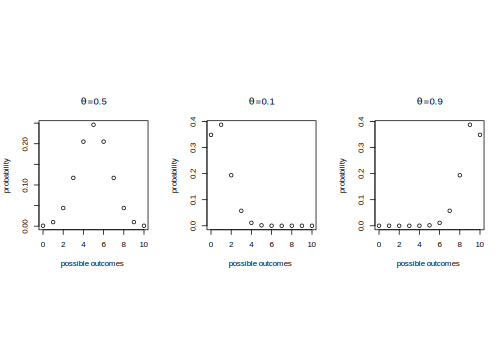
\includegraphics{Freq_CogSci_files/figure-latex/binomplot-1.pdf}
\caption{\label{fig:binomplot}Probability mass functions of a binomial distribution assuming 10 trials, with 50\%, 10\%, and 90\% probability of success.}
\end{figure}

The probability mass function for the binomial is written as follows.

\begin{equation}
\hbox{Binomial}(k|n,\theta) = 
\binom{n}{k} \theta^{k} (1-\theta)^{n-k}
\end{equation}

Here, \(n\) represents the total number of trials, \(k\) the number of successes, and \(\theta\) the probability of success. The term \(\binom{n}{k}\), pronounced n-choose-k, represents the number of ways in which one can choose \(k\) successes out of \(n\) trials. For example, 1 success out of 10 can occur in 10 possible ways: the very first trial could be a 1, the second trial could be a 1, etc.
The term \(\binom{n}{k}\) expands to \(\frac{n!}{k!(n-k)!}\); the exclamation mark is the factorial (e.g., \(3!=3\times 2\times 1\)). In \texttt{R}, \(\binom{n}{k}\) is computed using the function \texttt{choose(n,k)}, with \(n\) and \(k\) representing positive integer values.

\hypertarget{the-mean-and-variance-of-the-binomial-distribution}{%
\subsection{The mean and variance of the Binomial distribution}\label{the-mean-and-variance-of-the-binomial-distribution}}

It is possible to analytically compute the mean and variance of the PMF associated with the Binomial random variable \(Y\). Without getting into the details of how these are derived mathematically, we just state here that the mean of \(Y\) (also called the expectation, conventionally written \(E[Y]\)) and variance of \(Y\) (written \(Var(Y)\)) of a Binomial distribution with parameter \(\theta\) and \(n\) trials are \(E[Y] = n\theta\) and \(Var(Y) = n\theta (1-\theta)\).

Of course, we always know \(n\) (because we decide on the number of trials ourselves), but in real experimental situations we never know the true value of \(\theta\). But \(\theta\) can be estimated from the data. From the observed data, we can compute the estimate of \(\theta\), \(\hat \theta=k/n\). The quantity \(\hat \theta\) is the observed proportion of successes, and is called the \textbf{maximum likelihood estimate} of the true (but unknown mean). Once we have estimated \(\theta\) in this way, we can also obtain an estimate (also a maximum likelihood estimate) of the variance by computing \(n\hat\theta (1-\hat\theta)\). These estimates are then used for statistical inference.

What does the term ``maximum likelihood estimate'' mean? The term \textbf{likelihood} refers to the value of the Binomial distribution function for a particular value of \(\theta\), once we have observed some data. For example, suppose you record \(n=10\) trials, and observe \(k=7\) successes. What is the probability of observing \(7\) successes out of \(10\)? We need the binomial distribution to compute this value:

\begin{equation}
\hbox{Binomial}(k=7|n=10,\theta) = 
\binom{10}{7} \theta^{7} (1-\theta)^{10-7}
\end{equation}

Once we have observed the data, both \(n\) and \(k\) are fixed. The only variable in the above equation now is \(\theta\): the above function is now only dependent on the value of \(\theta\). When the data are fixed, the probability mass function is only dependent on the value of the parameter \(\theta\), and is called a \textbf{likelihood function}. It is therefore often expressed as a function of \(\theta\):

\(p( y | \theta ) = p( k=7, n=10 | \theta) = \mathcal{L}(\theta)\)

The vertical bar notation above should be read as saying that, given some data \(y\) (which in the binomial case will be \(k\) ``successes'' in \(n\) trials), the function returns a value for different values of \(\theta\).

If we now plot this function for all possible values of \(\theta\), we get the plot shown in Figure \ref{fig:binomlik}. We will show below how to compute this function for different values of \(\theta\).

\begin{figure}
\centering
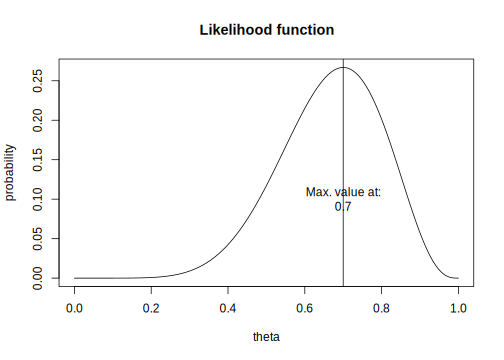
\includegraphics{Freq_CogSci_files/figure-latex/binomlik-1.pdf}
\caption{\label{fig:binomlik}The likelihood function for 7 successes out of 10.}
\end{figure}

What is important about this plot is that it shows that, given the data, the maximum point is at the point \(0.7\), which corresponds to the estimated mean using the formula shown above: \(k/n = 7/10\). Thus, the maximum likelihood estimate (MLE) gives us the most likely value of the parameter \(\theta\) given the data. It is crucial to note here that the phrase ``most likely'' does not mean that the MLE from a \emph{particular} sample of data invariably gives us an accurate estimate of \(\theta\). For example, if we run our experiment for \(10\) trials and get \(1\) success out of \(10\), the MLE is \(0.10\). We could have happened to observe only one success out of ten even if the true \(\theta\) were \(0.5\). The MLE would however give an accurate estimate of the true parameter \(\theta\) as \(n\) approaches infinity.

\hypertarget{what-information-does-a-probability-distribution-provide}{%
\subsection{What information does a probability distribution provide?}\label{what-information-does-a-probability-distribution-provide}}

What good is a probability mass function? We consider this question next. A lot of important information can be extracted from a PMF.

\hypertarget{compute-the-probability-of-a-particular-outcome-discrete-case-only}{%
\subsubsection{Compute the probability of a particular outcome (discrete case only)}\label{compute-the-probability-of-a-particular-outcome-discrete-case-only}}

The Binomial distribution shown in Figure \ref{fig:binomplot} already displays the probability of each possible outcome under a different value for \(\theta\). In \texttt{R}, there is a built-in function that allows us to calculate \(P(Y=k)\), the probability in the random variable \(Y\) of \(k\) successes out of \(n\), given a particular value of \(k\) (this number constitutes our data), the number of trials \(n\), and given a particular value of \(\theta\); this is the \texttt{dbinom} function. For example, the probability of 5 successes out of 10 when \(\theta\) is \(0.5\) is:

\begin{Shaded}
\begin{Highlighting}[]
\NormalTok{(prob<-}\KeywordTok{dbinom}\NormalTok{(}\DecValTok{5}\NormalTok{,}\DataTypeTok{size=}\DecValTok{10}\NormalTok{,}\DataTypeTok{prob=}\FloatTok{0.5}\NormalTok{))}
\end{Highlighting}
\end{Shaded}

\begin{verbatim}
## [1] 0.2461
\end{verbatim}

To be completely explicit, we can write this probability as \(P(k=5|n=10,\theta=0.5)=0.246\); when \(n\) and \(\theta\) are clear from context, we can also write simply \(P(k=5)\).

The probabilities of success when \(\theta\) is 0.1 or 0.7 can be computed by replacing 0.5 above by each of these probabilities:

\begin{Shaded}
\begin{Highlighting}[]
\KeywordTok{dbinom}\NormalTok{(}\DecValTok{5}\NormalTok{,}\DataTypeTok{size=}\DecValTok{10}\NormalTok{,}\DataTypeTok{prob=}\FloatTok{0.1}\NormalTok{)}
\end{Highlighting}
\end{Shaded}

\begin{verbatim}
## [1] 0.001488
\end{verbatim}

\begin{Shaded}
\begin{Highlighting}[]
\KeywordTok{dbinom}\NormalTok{(}\DecValTok{5}\NormalTok{,}\DataTypeTok{size=}\DecValTok{10}\NormalTok{,}\DataTypeTok{prob=}\FloatTok{0.7}\NormalTok{)}
\end{Highlighting}
\end{Shaded}

\begin{verbatim}
## [1] 0.1029
\end{verbatim}

One can alternatively run the above command in one shot; one can give a range of probabilities, and get the probability of 5 successes out of 10 for these different probabilities:

\begin{Shaded}
\begin{Highlighting}[]
\KeywordTok{dbinom}\NormalTok{(}\DecValTok{5}\NormalTok{,}\DataTypeTok{size=}\DecValTok{10}\NormalTok{,}\DataTypeTok{prob=}\KeywordTok{c}\NormalTok{(}\FloatTok{0.1}\NormalTok{,}\FloatTok{0.7}\NormalTok{))}
\end{Highlighting}
\end{Shaded}

\begin{verbatim}
## [1] 0.001488 0.102919
\end{verbatim}

The above command prints out the probability of 5 successes out of 10, when \(\theta=0.1\) and \(\theta=0.7\).

\hypertarget{compute-the-cumulative-probability-of-k-or-less-more-than-k-successes}{%
\subsubsection{Compute the cumulative probability of k or less (more) than k successes}\label{compute-the-cumulative-probability-of-k-or-less-more-than-k-successes}}

Instead of the probability of obtaining a given number of successes we could be interested in knowing the cumulative probability of obtaining 1 or less, or 2 or less successes. Formally, we will write this cumulative probability as \(F(2)\), and more generally, as \(F(k)\), for a particular value of \(k\). Thus, \(F(k)=P(Y\leq k)\).

We can compute this cumulative probability with the \texttt{dbinom} function, through a simple summation procedure:

\begin{Shaded}
\begin{Highlighting}[]
\CommentTok{## the cumulative probability of obtaining}
\CommentTok{## 0, 1, or 2 successes out of 10,}
\CommentTok{## with theta=0.5:}
\KeywordTok{dbinom}\NormalTok{(}\DecValTok{0}\NormalTok{,}\DataTypeTok{size=}\DecValTok{10}\NormalTok{,}\DataTypeTok{prob=}\FloatTok{0.5}\NormalTok{)}\OperatorTok{+}\KeywordTok{dbinom}\NormalTok{(}\DecValTok{1}\NormalTok{,}\DataTypeTok{size=}\DecValTok{10}\NormalTok{,}\DataTypeTok{prob=}\FloatTok{0.5}\NormalTok{)}\OperatorTok{+}
\StringTok{  }\KeywordTok{dbinom}\NormalTok{(}\DecValTok{2}\NormalTok{,}\DataTypeTok{size=}\DecValTok{10}\NormalTok{,}\DataTypeTok{prob=}\FloatTok{0.5}\NormalTok{)}
\end{Highlighting}
\end{Shaded}

\begin{verbatim}
## [1] 0.05469
\end{verbatim}

Mathematically, we could write the above summation as:

\begin{equation}
\sum_{k=0}^2 \binom{n}{k} \theta^{k} (1-\theta)^{n-k} 
\end{equation}

An alternative to the cumbersome addition in the R code above is this more compact statement, which closely mimics the above mathematical expression:

\begin{Shaded}
\begin{Highlighting}[]
\KeywordTok{sum}\NormalTok{(}\KeywordTok{dbinom}\NormalTok{(}\DecValTok{0}\OperatorTok{:}\DecValTok{2}\NormalTok{,}\DataTypeTok{size=}\DecValTok{10}\NormalTok{,}\DataTypeTok{prob=}\FloatTok{0.5}\NormalTok{))}
\end{Highlighting}
\end{Shaded}

\begin{verbatim}
## [1] 0.05469
\end{verbatim}

\texttt{R} has a built-in function called \texttt{pbinom} that does this summation for us. If we want to know the probability of \(2\) or less successes as in the above example, we can write:

\begin{Shaded}
\begin{Highlighting}[]
\KeywordTok{pbinom}\NormalTok{(}\DecValTok{2}\NormalTok{,}\DataTypeTok{size=}\DecValTok{10}\NormalTok{,}\DataTypeTok{prob=}\FloatTok{0.5}\NormalTok{,}\DataTypeTok{lower.tail=}\OtherTok{TRUE}\NormalTok{)}
\end{Highlighting}
\end{Shaded}

\begin{verbatim}
## [1] 0.05469
\end{verbatim}

The specification \texttt{lower.tail=TRUE} ensures that the summation goes from \(2\) to numbers smaller than \(2\) (which lie in the lower tail of the distribution in Figure \ref{fig:binomplot}). If we wanted to know what the probability is of obtaining \(2\) or more successes out of \(10\), we can set \texttt{lower.tail} to \texttt{FALSE}:

\begin{Shaded}
\begin{Highlighting}[]
\KeywordTok{pbinom}\NormalTok{(}\DecValTok{2}\NormalTok{,}\DataTypeTok{size=}\DecValTok{10}\NormalTok{,}\DataTypeTok{prob=}\FloatTok{0.5}\NormalTok{,}\DataTypeTok{lower.tail=}\OtherTok{FALSE}\NormalTok{)}
\end{Highlighting}
\end{Shaded}

\begin{verbatim}
## [1] 0.9453
\end{verbatim}

The cumulative distribution function or CDF, \(F(k)\), can be plotted by computing the cumulative probabilities for any value \(k\) or less than \(k\), where \(k\) ranges from \(0\) to \(10\) in our running example. The CDF is shown in Figure \ref{fig:binomcdf}.

\begin{figure}
\centering
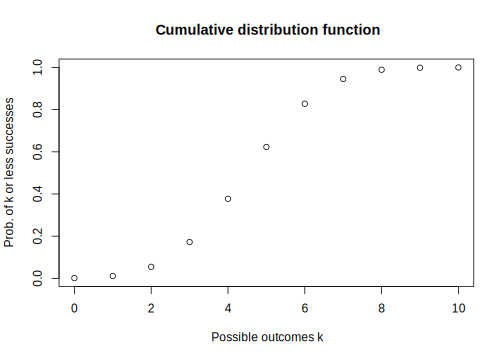
\includegraphics{Freq_CogSci_files/figure-latex/binomcdf-1.pdf}
\caption{\label{fig:binomcdf}The cumulative distribution function for a binomial distribution assuming 10 trials, with 50\% probability of success.}
\end{figure}

\hypertarget{compute-the-inverse-of-the-cumulative-distribution-function-the-quantile-function}{%
\subsubsection{Compute the inverse of the cumulative distribution function (the quantile function)}\label{compute-the-inverse-of-the-cumulative-distribution-function-the-quantile-function}}

We can also find out the value of the variable \(k\) (the quantile) such that the probability of obtaining \(k\) or less than \(k\) successes is some specific probability value \(p\). If we switch the x and y axes of Figure \ref{fig:binomcdf}, we obtain another very useful function, the inverse CDF.

The inverse of the CDF (known as the quantile function in R because it returns the quantile, the value k) is available in R as the function \texttt{qbinom}. The usage is as follows: to find out what the value \(k\) of the outcome is such that the probability of obtaining \(k\) or less successes is \(0.37\), type:

\begin{Shaded}
\begin{Highlighting}[]
\KeywordTok{qbinom}\NormalTok{(}\FloatTok{0.37}\NormalTok{,}\DataTypeTok{size=}\DecValTok{10}\NormalTok{,}\DataTypeTok{prob=}\FloatTok{0.5}\NormalTok{)}
\end{Highlighting}
\end{Shaded}

\begin{verbatim}
## [1] 4
\end{verbatim}

\hypertarget{generate-random-data-from-a-hboxbinomialntheta-distribution}{%
\subsubsection{\texorpdfstring{Generate random data from a \(\hbox{Binomial}(n,\theta)\) distribution}{Generate random data from a \textbackslash{}hbox\{Binomial\}(n,\textbackslash{}theta) distribution}}\label{generate-random-data-from-a-hboxbinomialntheta-distribution}}

We can generate random simulated data from a Binomial distribution by specifying the number of trials and the probability of success \(\theta\). In \texttt{R}, we do this in the following way:

\begin{Shaded}
\begin{Highlighting}[]
\KeywordTok{rbinom}\NormalTok{(}\DataTypeTok{n=}\DecValTok{10}\NormalTok{,}\DataTypeTok{size=}\DecValTok{1}\NormalTok{,}\DataTypeTok{prob=}\FloatTok{0.5}\NormalTok{)}
\end{Highlighting}
\end{Shaded}

\begin{verbatim}
##  [1] 1 0 1 1 0 1 0 1 0 1
\end{verbatim}

The above code generates a sequences of 10 randomly generated \(1\)'s and \(0\)'s. Each of the 1's and 0's is called an outcome coming from a Bernoulli distribution. In other words, a Bernoulli distribution is just a Binomial distribution with size=1, i.e., a single trial.

Repeatedly run the above code; you will get different sequences of 1's and 0's each time. For each generated sequence, one can calculate the number of successes by just summing up the vector, or computing its mean and multiplying by the number of trials, here \(10\):

\begin{Shaded}
\begin{Highlighting}[]
\NormalTok{y<-}\KeywordTok{rbinom}\NormalTok{(}\DataTypeTok{n=}\DecValTok{10}\NormalTok{,}\DataTypeTok{size=}\DecValTok{1}\NormalTok{,}\DataTypeTok{prob=}\FloatTok{0.5}\NormalTok{)}
\KeywordTok{mean}\NormalTok{(y)}\OperatorTok{*}\DecValTok{10}\NormalTok{ ; }\KeywordTok{sum}\NormalTok{(y)}
\end{Highlighting}
\end{Shaded}

\begin{verbatim}
## [1] 6
\end{verbatim}

\begin{verbatim}
## [1] 6
\end{verbatim}

We can think of the above as 10 Bernoulli trials, or a single Binomial trial of size 10. When we see the data in this way, the syntax and output changes:

\begin{Shaded}
\begin{Highlighting}[]
\NormalTok{(y<-}\KeywordTok{rbinom}\NormalTok{(}\DataTypeTok{n=}\DecValTok{1}\NormalTok{,}\DataTypeTok{size=}\DecValTok{10}\NormalTok{,}\DataTypeTok{prob=}\FloatTok{0.5}\NormalTok{))}
\end{Highlighting}
\end{Shaded}

\begin{verbatim}
## [1] 5
\end{verbatim}

Seen as a Binomial experiment with size 10, the function returns the number of successes in a particular experiment with size 10.

Next, let's take a look at an example of a continuous random variable.

\hypertarget{continuous-random-variables-an-example-using-the-normal-distribution}{%
\section{Continuous random variables: An example using the Normal distribution}\label{continuous-random-variables-an-example-using-the-normal-distribution}}

We will now revisit the idea of a random variable using a continuous distribution as an example. Imagine that you have reading time data, represented as a vector \(y\). The data \(y\) are measured in milliseconds and are assumed to come from (i.e., assumed to be generated by) a random variable \(Y\) that has as PDF the Normal distribution (this is not a realistic assumption; we will come up with a more realistic assumption later). We will write the above statement compactly as follows:

\begin{equation}
Y \sim Normal(\mu,\sigma)
\end{equation}

This expression should be read as: the random variable \(Y\) has PDF \(Normal(\mu,\sigma)\). The random variable \(Y\) refers to an abstract mathematical object; specific instances of observed (or simulated) data will be referred to with the lower-case equivalent of the random variable; here, \(y\) can refer to a particular data-point or a vector of data (the context will make it clear whether we are talking about a single data point or a vector of data). A further important notational detail: in statistics textbooks, you will often see the Normal distribution represented in terms of the mean and the variance (\(\sigma^2\)) instead of the standard deviation \(\sigma\) that we use here. We have consciously chosen to use the standard deviation in the Normal distribution; this is because \texttt{R} uses the standard deviation and not the variance to define a normal distribution.

An important assumption we make here is that each data point in the vector of data \(y\) is independent of the others. Often, we express this assumption by saying that we have ``independent and identically distributed data''; this is abbreviated as ``i.i.d''. One can be very explicit about this and write:

\begin{equation}
Y \stackrel{iid}{\sim}  Normal(\mu,\sigma)
\end{equation}

The probability density function (PDF) of the Normal distribution is defined as follows:

\begin{equation}
Normal(y|\mu,\sigma)=f(y)= \frac{1}{\sqrt{2\pi \sigma^2}} \exp \left(-\frac{(y-\mu)^2}{2\sigma^2} \right)
\end{equation}

Here, \(\mu\) is the mean, and \(\sigma\) is the standard deviation of the Normal distribution that the reading times have been sampled from. To display this function, we would have to decide on specific values for \(\mu\) and \(\sigma\) and then input the \(y\) value into the function to plot it. It may be instructive to write this function ``by hand'' and then plot it. We just choose some default values for \(\mu\) and \(\sigma\) here.

\begin{Shaded}
\begin{Highlighting}[]
\NormalTok{my_normal<-}\ControlFlowTok{function}\NormalTok{(}\DataTypeTok{y=}\OtherTok{NULL}\NormalTok{,}\DataTypeTok{mu=}\DecValTok{500}\NormalTok{,}\DataTypeTok{sigma=}\DecValTok{100}\NormalTok{)\{}
\NormalTok{  (}\DecValTok{1}\OperatorTok{/}\KeywordTok{sqrt}\NormalTok{(}\DecValTok{2}\OperatorTok{*}\NormalTok{pi}\OperatorTok{*}\NormalTok{sigma}\OperatorTok{^}\DecValTok{2}\NormalTok{))}\OperatorTok{*}\KeywordTok{exp}\NormalTok{(}\OperatorTok{-}\NormalTok{(y}\OperatorTok{-}\NormalTok{mu)}\OperatorTok{^}\DecValTok{2}\OperatorTok{/}\NormalTok{(}\DecValTok{2}\OperatorTok{*}\NormalTok{sigma}\OperatorTok{^}\DecValTok{2}\NormalTok{))}
\NormalTok{\}}
\NormalTok{y<-}\KeywordTok{seq}\NormalTok{(}\DecValTok{100}\NormalTok{,}\DecValTok{900}\NormalTok{,}\DataTypeTok{by=}\FloatTok{0.01}\NormalTok{)}
\KeywordTok{plot}\NormalTok{(y,}\KeywordTok{my_normal}\NormalTok{(}\DataTypeTok{y=}\NormalTok{y),}\DataTypeTok{type=}\StringTok{"l"}\NormalTok{)}
\end{Highlighting}
\end{Shaded}

\begin{figure}
\centering
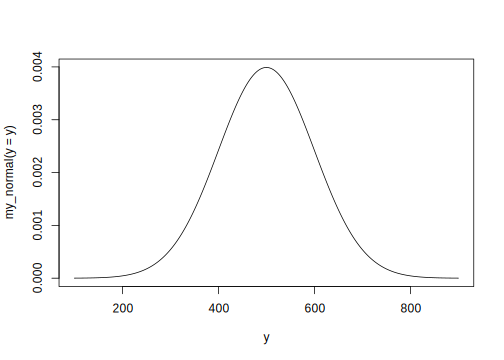
\includegraphics{Freq_CogSci_files/figure-latex/mynormdistrn-1.pdf}
\caption{\label{fig:mynormdistrn}Creating one's own Normal distribution function.}
\end{figure}

Just like the \texttt{dbinom} function we saw earlier, there is a built-in function in \texttt{R} called \texttt{dnorm} that will allow us to display the Normal distribution.
Using \texttt{dnorm}, we can visualize the Normal distribution for particular values of \(\mu\) and \(\sigma\) as a PDF. Analogously to the discrete example we saw earlier, we can also plot the corresponding CDF (using \texttt{pnorm}), and the inverse CDF (using \texttt{qnorm}). See Figure \ref{fig:normdistrn}.

In the continuous case, the PDF gives us something called the \emph{density} for each possible value of our data \(y\); ``density'' here is not the probability, rather is it giving us a non-negative number that is the value of the function \(f(y)\) in the equation immediately above. We will return to the concept of density when we do an exercise on \emph{maximum likelihood estimation}.

As in the discrete case, the CDF tells us the probability of observing a value like y or some value less than that (written: \(P(Y<y)\)); and the inverse CDF gives us the quantile \(y\) such that \(P(Y<y)\) is some specific value between 0 and 1. The PDF, CDF, and inverse CDF are three different ways of looking at the same information.

\begin{figure}
\centering
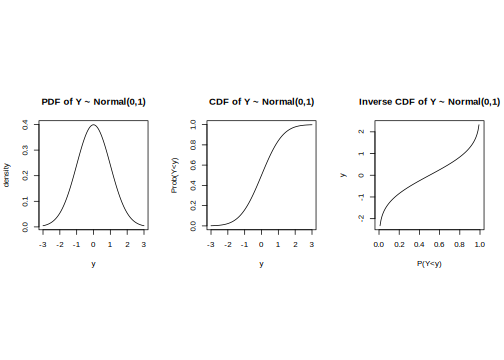
\includegraphics{Freq_CogSci_files/figure-latex/normdistrn-1.pdf}
\caption{\label{fig:normdistrn}The PDF, CDF, and inverse CDF for the \(Normal(\mu=0,\sigma=1)\).}
\end{figure}

One important fact about the normal distribution is that 95\% of the probability mass is covered by approximately plus/minus 1.96 times the standard deviation about the mean. Thus, the range \(\mu\pm 1.96\times \sigma\) will cover approximately 95\% of the area under the curve. We will approximate this by talking about \(\mu\pm 2\times \sigma\).

As in the discrete example, the PDF, CDF, and inverse of the CDF allow us to ask questions like:

\begin{itemize}
\tightlist
\item
  \textbf{What is the probability of observing values between some range \(a\) and \(b\) from a Normal distribution with mean \(\mu\) and standard deviation \(\sigma\)}? We can compute the probability of the random variable lying between 1 and minus infinity:
\end{itemize}

\begin{Shaded}
\begin{Highlighting}[]
\KeywordTok{pnorm}\NormalTok{(}\DecValTok{1}\NormalTok{,}\DataTypeTok{mean=}\DecValTok{0}\NormalTok{,}\DataTypeTok{sd=}\DecValTok{1}\NormalTok{)}
\end{Highlighting}
\end{Shaded}

\begin{verbatim}
## [1] 0.8413
\end{verbatim}

\begin{figure}
\centering
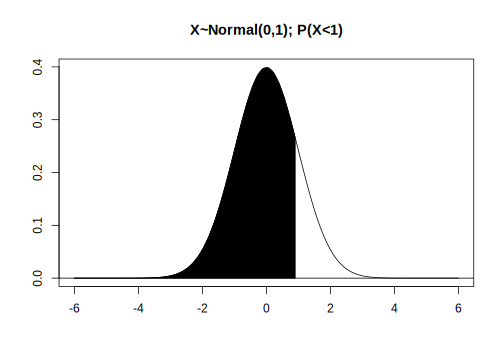
\includegraphics{Freq_CogSci_files/figure-latex/auc-1.pdf}
\caption{\label{fig:auc}The area under the curve between 1 and minus infinity in a Normal distribution with mean 0 and standard deviation 1.}
\end{figure}

Notice here that the probability of any point value in a PDF is always 0. This is because the probability in a continuous probability distribution is defined to be the area under the curve, and the area under the curve at any single point on the x-axis is always 0. The implication here is that we can only ask about probabilities between a range of values; e.g., the probability that \(Y\) lies between \(a\) and \(b\), or \(P(a<Y<b)\), where \(a\neq b\). Also, notice that \(P(a<Y<b)\) and \(P(a\leq Y\leq b)\) will be the same probability, because of the fact that \(P(Y=a)\) or \(P(Y=b)\) both equal 0.

\begin{itemize}
\tightlist
\item
  \textbf{What is the quantile \(q\) such that the probability is \(p\) of observing that value \(q\) or something less (or more) than it}? For example, we can work out the quantile \(q\) such that the probability of observing \(q\) or something less than it is 0.975, in the Normal(500,100) distribution. Formally, we would write this as \(F(a)=P(Y<a)\).
\end{itemize}

\begin{Shaded}
\begin{Highlighting}[]
\KeywordTok{qnorm}\NormalTok{(}\FloatTok{0.975}\NormalTok{,}\DataTypeTok{mean=}\DecValTok{500}\NormalTok{,}\DataTypeTok{sd=}\DecValTok{100}\NormalTok{)}
\end{Highlighting}
\end{Shaded}

\begin{verbatim}
## [1] 696
\end{verbatim}

The above output says that the probability that the random variable is less than \(q=696\) is 97.5\%.

\begin{itemize}
\tightlist
\item
  \textbf{Generating simulated data}. Given a vector of \(n\) independent and identically distributed data \(y\), i.e., given that each data point is being generated independently from \(Y \sim Normal(\mu,\sigma)\) for some values of the parameters \(\mu,\sigma\), the maximum likelihood estimates for the expectation and variance are
\end{itemize}

\begin{equation}
\bar{y} =  \frac{\sum_{i=1}^n y_i}{n} 
\end{equation}

\begin{equation}
Var(y) = \frac{\sum_{i=1}^n (y_i-
\bar{y})^2}{n}
\end{equation}

As an aside, keep in mind that the formula for variance in \texttt{R} is slightly different: it divides by \(n-1\) instead of \(n\).

\begin{equation}
Var(y) = \frac{\sum_{i=1}^n (y_i-
\bar{y})^2}{n-1}
\end{equation}

The reason for this difference is simply that division by \(n-1\) leads to a so-called unbiased estimate of the variance.

Let's simulate some sample data from a Normal distribution and compute estimates of the mean and variance.\\
Let's generate \(10\) data points using the \texttt{rnorm} function, and then compute the mean and variance from the simulated data:

\begin{Shaded}
\begin{Highlighting}[]
\NormalTok{y<-}\KeywordTok{rnorm}\NormalTok{(}\DecValTok{10}\NormalTok{,}\DataTypeTok{mean=}\DecValTok{500}\NormalTok{,}\DataTypeTok{sd=}\DecValTok{100}\NormalTok{)}
\KeywordTok{mean}\NormalTok{(y);}\KeywordTok{var}\NormalTok{(y)}
\end{Highlighting}
\end{Shaded}

\begin{verbatim}
## [1] 543.1
\end{verbatim}

\begin{verbatim}
## [1] 8037
\end{verbatim}

As mentioned earlier, depending on the sample size, the sample mean and sample variance \emph{from a particular sample} may or may not be close to the true values of the respective parameters, despite the fact that these are \emph{maximum likelihood estimates}. The estimates of the mean and variance from a particular sample will be close to the true values of the parameters as the sample size goes to infinity.

\hypertarget{other-common-distributions}{%
\section{Other common distributions}\label{other-common-distributions}}

Here, we briefly present some of the distributions that we will need or use in this book. Throughout, we assume independent and identically distributed data.

\hypertarget{the-t-distribution}{%
\subsection{The t-distribution}\label{the-t-distribution}}

This continuous distribution, written \(t(n-1)\), take as a parameter the degrees of freedom (roughly, the sample size \(n\)) minus one. As the degrees of freedom increase to infinity (as the sample size increases to infinity), the distribution approaches the Normal distribution with mean 0 and standard deviation 1.

The pdf is:

\begin{equation}
f(x) = \frac{\Gamma((n+1)/2)}{\sqrt{n\pi} \Gamma(n/2)} (1+x^2/n)^{-(n+1)/2} \hbox{  Support: } x \in (-\infty, \infty)
\end{equation}

\(\Gamma()\) is the Gamma function: \(\Gamma(n)=n-1!\).
The mean of the t-distribution is \(0\) if \(n>1\) and variance \(\frac{n}{n-2}\) if \(n>2\).

The t-distribution becomes the Cauchy distribution if \(n=2\). The Cauchy distribution has no mean or variance defined for it.

There are four functions in \texttt{R} that serve the same purpose as the \texttt{dnorm}, \texttt{pnorm}, \texttt{qnorm}, \texttt{rnorm} functions for the Normal:
\texttt{dt}, \texttt{pt}, \texttt{qt}, \texttt{rt}.

\hypertarget{the-gamma-distribution}{%
\subsection{The Gamma distribution}\label{the-gamma-distribution}}

The distribution is written \(Gamma(a,b)\), and takes two parameters, \(a\) and \(b\).

The pdf is:

\begin{equation}
f(x) = \frac{1}{\Gamma(a)}(b x)^ae^{-b x}\frac{1}{x} \hbox{  Support: } x \in (0, \infty)
\end{equation}

The mean is \(\frac{a}{b}\) and the variance is \(\frac{a}{b^2}\).

\hypertarget{the-exponential-distribution}{%
\subsection{The Exponential distribution}\label{the-exponential-distribution}}

The Exponential, written \(Exp(\lambda)\), takes the parameter \(\lambda\) and has the PDF:

\begin{equation}
f(x) = \lambda e^{-\lambda x} \hbox{  Support: } x \in (0, \infty)
\end{equation}

Its mean is \(\frac{1}{\lambda}\) and variance \(\frac{1}{\lambda^2}\).

\hypertarget{bivariate-and-multivariate-distributions}{%
\section{Bivariate and multivariate distributions}\label{bivariate-and-multivariate-distributions}}

So far, we have only discussed univariate distributions. It is also possible to specify distributions with two or more dimensions.

Understanding bivariate (and, more generally, multivariate) distributions, and knowing how to simulate data from such distributions, is vital for us because linear mixed models crucially depend on such distributions. If we want to understand linear mixed models, we have to understand multivariate distributions.

\hypertarget{example-1-discrete-bivariate-distributions}{%
\subsection{Example 1: Discrete bivariate distributions}\label{example-1-discrete-bivariate-distributions}}

Starting with the discrete case, consider the discrete bivariate distribution shown below. These are data from an experiment where, inter alia, in each trial a Likert acceptability rating and a response accuracy (to a yes-no question) were recorded (the data are from a study by \citet{AnnaLphd}, used with permission here).

Figure \ref{fig:bivardiscrete} shows the \emph{joint probability mass function} of two random variables X and Y. The random variable X consists of 7 possible values (this is the 1-7 Likert response scale), and the random variable Y is response accuracy, with 0 representing incorrect responses, and 1 representing correct responses.

\begin{Shaded}
\begin{Highlighting}[]
\NormalTok{agrmt<-}\KeywordTok{read.csv}\NormalTok{(}\StringTok{"data/agrmt_discrete_binomial.csv"}\NormalTok{)}
\NormalTok{rating0<-}\KeywordTok{table}\NormalTok{(}\KeywordTok{subset}\NormalTok{(agrmt,accuracy}\OperatorTok{==}\DecValTok{0}\NormalTok{)}\OperatorTok{$}\NormalTok{rating)}
\NormalTok{rating1<-}\KeywordTok{table}\NormalTok{(}\KeywordTok{subset}\NormalTok{(agrmt,accuracy}\OperatorTok{==}\DecValTok{1}\NormalTok{)}\OperatorTok{$}\NormalTok{rating)}

\NormalTok{ratingsbivar<-}\KeywordTok{data.frame}\NormalTok{(}\DataTypeTok{rating0=}\NormalTok{rating0,}
                         \DataTypeTok{rating1=}\NormalTok{rating1)}

\NormalTok{ratingsbivar<-ratingsbivar[,}\KeywordTok{c}\NormalTok{(}\DecValTok{2}\NormalTok{,}\DecValTok{4}\NormalTok{)]}
\KeywordTok{colnames}\NormalTok{(ratingsbivar)<-}\KeywordTok{c}\NormalTok{(}\DecValTok{0}\NormalTok{,}\DecValTok{1}\NormalTok{)}
\KeywordTok{library}\NormalTok{ (MASS)}

\CommentTok{## function from bivariate package:}
\NormalTok{f <-}\StringTok{ }\KeywordTok{cbvpmf}\NormalTok{ (ratingsbivar)}
\KeywordTok{plot}\NormalTok{ (f, }\OtherTok{TRUE}\NormalTok{,}
       \DataTypeTok{arrows=}\OtherTok{FALSE}\NormalTok{)}
\end{Highlighting}
\end{Shaded}

\begin{figure}
\centering
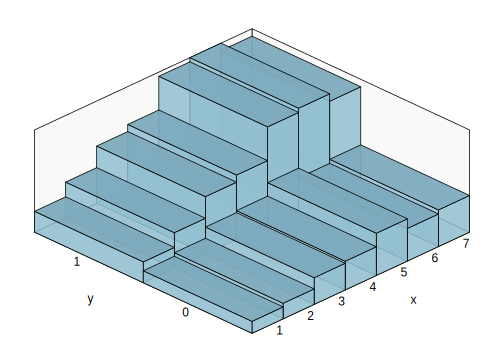
\includegraphics{Freq_CogSci_files/figure-latex/bivardiscrete-1.pdf}
\caption{\label{fig:bivardiscrete}Example of a discrete bivariate distribution. In these data, in every trial, two pieces of information were collected: Likert responses and yes-no question responses. The random variable X represents Likert scale responses on a scale of 1-7. and the random variable Y represents 0, 1 (incorrect, correct) responses to comprehension questions.}
\end{figure}

One can also display the figure as a table.

\begin{Shaded}
\begin{Highlighting}[]
\NormalTok{probs<-}\KeywordTok{attr}\NormalTok{(f,}\StringTok{"p"}\NormalTok{)}
\KeywordTok{t}\NormalTok{(probs)}
\end{Highlighting}
\end{Shaded}

\begin{verbatim}
##      [,1]    [,2]    [,3]    [,4]    [,5]    [,6]
## 0 0.01792 0.02328 0.04004 0.04306 0.06331 0.04888
## 1 0.03119 0.05331 0.08566 0.09637 0.14688 0.15317
##      [,7]
## 0 0.05493
## 1 0.14199
\end{verbatim}

For each possible value of X and Y, we have a joint probability. Given such a bivariate distribution, there are two useful quantities we can compute: the \emph{marginal} distributions (\(p_{X}\) and \(p_Y\)), and the \emph{conditional} distributions (\(p_{X|Y}\) and \(p_{Y|X}\)).\\
The table below shows the joint probability mass function \(p_{X,Y}(x,y)\).

\begin{table}[!htbp] 
\begin{center}
\begin{tabular}{c|ccccccc}
$p_{X,Y}$ & x=1 & x=2 & x=3 & x=4 & x=5 & x=6 & x=7\\
\hline
y = 0 & 0.018 & 0.023 & 0.040 & 0.043 & 0.063 & 0.049 & 0.055\\
y = 1 & 0.031 & 0.053 & 0.086 & 0.096 &  0.147 & 0.153 &  0.142\\
\end{tabular}
\end{center}
\caption{The joint PMF for two random variables $X$ and $Y$.}\label{discretebivartable}
\end{table}

The marginal distribution \(p_Y\) is defined as follows. \(S_{X}\) is the support of X, i.e., all the possible values of X.

\begin{equation}
p_{Y}(y)=\sum_{x\in S_{X}}p_{X,Y}(x,y).\label{eq-marginal-pmf}
\end{equation}

Similarly, the marginal distribution \(p_X\) is defined as:

\begin{equation}
p_{X}(x)=\sum_{y\in S_{Y}}p_{X,Y}(x,y).\label{eq-marginal-pmf2}
\end{equation}

\(p_Y\) is easily computed, by summing up the values in each row; and \(p_X\) by summing up the values in each column. You can see why this is called the marginal distribution; the result appears in the margins of the table.

\begin{Shaded}
\begin{Highlighting}[]
\CommentTok{#P(Y)}
\NormalTok{(PY<-}\KeywordTok{rowSums}\NormalTok{(}\KeywordTok{t}\NormalTok{(probs)))}
\end{Highlighting}
\end{Shaded}

\begin{verbatim}
##      0      1 
## 0.2914 0.7086
\end{verbatim}

\begin{Shaded}
\begin{Highlighting}[]
\KeywordTok{sum}\NormalTok{(PY) }\CommentTok{## sums to 1}
\end{Highlighting}
\end{Shaded}

\begin{verbatim}
## [1] 1
\end{verbatim}

\begin{Shaded}
\begin{Highlighting}[]
\CommentTok{#P(X)}
\NormalTok{(PX<-}\KeywordTok{colSums}\NormalTok{(}\KeywordTok{t}\NormalTok{(probs)))}
\end{Highlighting}
\end{Shaded}

\begin{verbatim}
## [1] 0.04912 0.07658 0.12570 0.13943 0.21020 0.20205
## [7] 0.19693
\end{verbatim}

\begin{Shaded}
\begin{Highlighting}[]
\KeywordTok{sum}\NormalTok{(PX) }\CommentTok{## sums to 1}
\end{Highlighting}
\end{Shaded}

\begin{verbatim}
## [1] 1
\end{verbatim}

The marginal probabilities sum to 1, as they should. The table below shows the marginal probabilities.

\small
\begin{table}[!htbp]
\begin{center}
\begin{tabular}{c|ccccccc|c}
$p_{X,Y}$ & x=1 & x=2 & x=3 & x=4 & x=5 & x=6 & x=7 & P(Y)\\
\hline
y = 0 & 0.018 & 0.023 & 0.040 & 0.043 & 0.063 & 0.049 & 0.055 &  \textbf{0.291}\\
y = 1 & 0.031 & 0.053 & 0.086 & 0.096 &  0.147 & 0.153 &  0.142 &  \textbf{0.709}\\
\hline
P(X) & \textbf{0.049} & \textbf{0.077} & \textbf{0.126} & \textbf{0.139} & \textbf{0.210} & \textbf{0.202} & \textbf{0.197}\\
\end{tabular}
\end{center}
\caption{The joint and marginal distributions of X and Y.}\label{discretebivartable2}
\end{table}
\normalsize

Notice that to compute the marginal distribution of X, one is summing over all the Ys; and to compute the marginal distribution of Y, one sums over all the X's. We say that we are \emph{marginalizing out} the random variable that we are summing over. One can visualize the two marginal distributions using barplots.

\begin{figure}
\centering
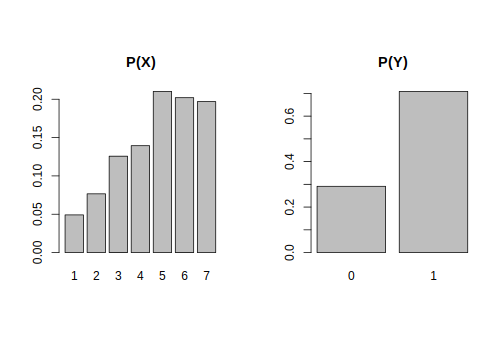
\includegraphics{Freq_CogSci_files/figure-latex/marginalprobs-1.pdf}
\caption{\label{fig:marginalprobs}Marginal distributions of X and Y.}
\end{figure}

For computing conditional distributions, recall that the conditional distribution of a random variable \(X\) given that \(Y=y\), where \(y\) is some specific (fixed) value, is:

\begin{equation}
p_{X\mid Y} (x\mid y) = \frac{p_{X,Y}(x,y)}{p_Y(y)} \quad \hbox{provided } p_Y(y)=P(Y=y)>0
\end{equation}

As an example, let's consider how \(p_{X\mid Y}\) would be computed.
The possible values of \(y\) are \(0,1\), and so we have to find the conditional distribution (defined above) for each of these values. I.e., we have to find \(p_{X\mid Y}(x\mid y=0)\), and \(p_{X\mid Y}(x\mid y=1)\).

Let's do the calculation for \(p_{X\mid Y}(x\mid y=0)\).

\begin{equation}
\begin{split}
p_{X\mid Y} (1\mid 0) =& \frac{p_{X,Y}(1,0)}{p_Y(0)}\\
    =&  \frac{0.018}{0.291}\\
    =& 0.0619
\end{split} 
\end{equation}

This conditional probability value will occupy the cell X=1, Y=0 in the table below summarizing the conditional probability distribution \(p_{X|Y}\). In this way, one can fill in the entire table, which will then represent the conditional distributions \(p_{X|Y=0}\) and \(p_{X|Y=1}\). The reader may want to take a few minutes to complete the table.

\begin{table}[!htbp]
\begin{center}
\begin{tabular}{c|ccccccc}
    & x=1 & x=2 & x=3 & x=4 & x=5 & x=6 & x=7\\ 
\hline  
$p_{X\mid Y}(x\mid y=0)$  & 0.0619 &  & & & & & \\
$p_{X\mid Y}(x\mid y=1)$  &  &  & & & & &  \\
\end{tabular}
\end{center}
\caption{The conditional probability distribution of X given Y.}
\label{XgivenY}
\end{table}

Similarly, one can construct a table that shows \(p_{Y|X}\).

\hypertarget{example-2-continuous-bivariate-distributions}{%
\subsection{Example 2: Continuous bivariate distributions}\label{example-2-continuous-bivariate-distributions}}

Consider now the continuous bivariate case; this time, we will use simulated data. Consider two normal random variables \(X\) and \(Y\), each of which coming from, for example, a Normal(0,1) distribution, with some correlation \(\rho\) between the two random variables.

A bivariate distribution for two random variables \(X\) and \(Y\), each of which comes from a normal distribution, is expressed in terms of the means and standard deviations of each of the two distributions, and the correlation \(\rho\) between them. The standard deviations and correlation are expressed in a special form of a \(2\times 2\) matrix called a variance-covariance matrix \(\Sigma\). If \(\rho_u\) is the correlation between the two random variables, and \(\sigma _{x}\) and \(\sigma _{y}\) the respective standard deviations, the variance-covariance matrix is written as:

\begin{equation}\label{eq:covmatfoundations}
\Sigma
=
\begin{pmatrix}
\sigma _{x}^2  & \rho\sigma _{x}\sigma _{y}\\
\rho\sigma _{x}\sigma _{y}    & \sigma _{y}^2\\
\end{pmatrix}
\end{equation}

The off-diagonals of this matrix contain the covariance between \(X\) and \(Y\).

The joint distribution of \(X\) and \(Y\) is defined as follows:

\begin{equation}\label{eq:jointpriordistfoundations}
\begin{pmatrix}
  X \\ 
  Y \\
\end{pmatrix}
\sim 
\mathcal{N}_2 \left(
\begin{pmatrix}
  0 \\
  0 \\
\end{pmatrix},
\Sigma
\right)
\end{equation}

The subscript on \(\mathcal{N}_2\) refers to the number of dimensions; if we had a multivariate distribution with three random variables, say X, Y, Z, the distribution would be \(\mathcal{N}_3\), and so on. The variance-covariance matrix for the three-dimensional distribution would be a \(3\times 3\) matrix, not a \(2\times 2\) matrix as above, and would contain three correlations (\(\rho_{X,Y},\rho_{X,Z},\rho_{Y,Z}\)).

Returning to the bivariate example, the joint PDF is written with reference to the two variables \(f_{X,Y}(x,y)\). It has the property that the area under the curve sums to 1. Formally, we would write this as a double integral: we are summing up the area under the curve for both dimensions X and Y. The integral symbol (\(\int\)) is just the continuous equivalent of the discrete summation symbol (\(\sum\)).

\begin{equation}
\iint_{S_{X,Y}} f_{X,Y}(x,y)\, dx dy = 1
\end{equation}

Here, the terms \(dx\) and \(dy\) express the fact that we are summing the area under the curve along the X axis and the Y axis.

The joint CDF would be written as follows. The equation below gives us the probability of observing a value like \((u,v)\) or some value smaller than that (i.e., some \((u',v')\), such that \(u'<u\) and \(v'<v\).

\begin{equation}
\begin{split}
F_{X,Y}(u,v) =& P(X<u,Y<v)\\
             =& \int_{-\infty}^u \int_{-\infty}^v f_{X,Y}(x,y)\, dy dx \hbox{ for } (x,y)\in \mathbb{R}^2\\
\end{split}
\end{equation}

As an aside, notice that the support for the normal distribution ranges from minus infinity to plus infinity. There can however be other PDFs with a more limited support; an example would be a normal distribution whose pdf \(f(x)\) is such that the lower bound is truncated at, say, 0. In such a case, the area under the range \(\int_{-\infty}^0 f(x) \, dx\) will be 0 because the range lies outside the support of the truncated normal distribution.

A visualization will help. The figures below show a bivariate distribution with correlation zero (Figure \ref{fig:zerocor}), a positive (Figure \ref{fig:poscor}) and a negative correlation (Figure \ref{fig:negcor}).

\begin{figure}
\centering
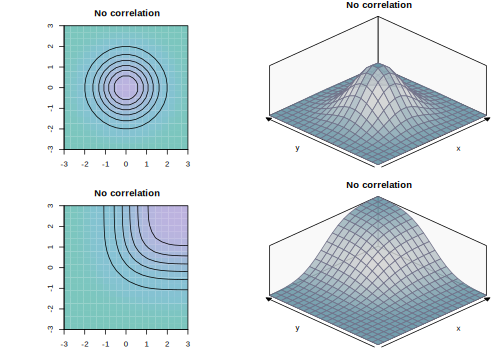
\includegraphics{Freq_CogSci_files/figure-latex/zerocor-1.pdf}
\caption{\label{fig:zerocor}A bivariate Normal distribution with zero correlation. Shown are four plots: the top-right plot shows the three-dimensional bivariate density, the top-left plot the contour plot of the distribution (seen from above). The lower plots show the cumulative distribution function from two views, as a three-dimensional plot and as a contour plot.}
\end{figure}

\begin{figure}
\centering
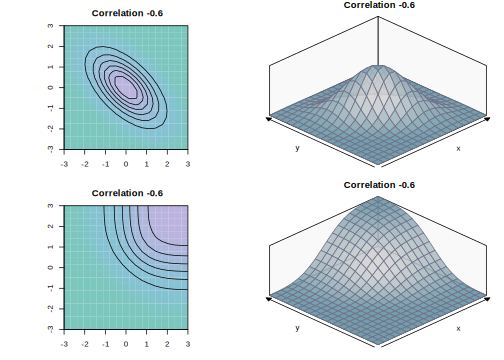
\includegraphics{Freq_CogSci_files/figure-latex/poscor-1.pdf}
\caption{\label{fig:poscor}A bivariate Normal distribution with a positive correlation of 0.6. Shown are four plots: the top-right plot shows the three-dimensional bivariate density, the top-left plot the contour plot of the distribution (seen from above). The lower plots show the cumulative distribution function from two views, as a three-dimensional plot and as a contour plot.}
\end{figure}

\begin{figure}
\centering
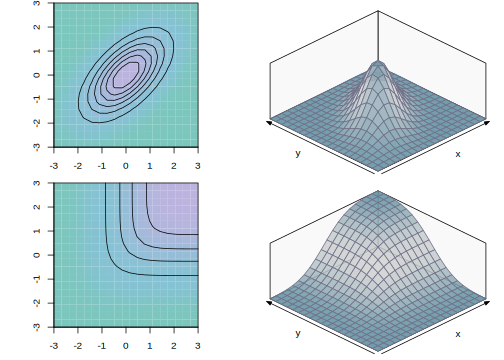
\includegraphics{Freq_CogSci_files/figure-latex/negcor-1.pdf}
\caption{\label{fig:negcor}A bivariate Normal distribution with a negative correlation of -0.6. Shown are four plots: the top-right plot shows the three-dimensional bivariate density, the top-left plot the contour plot of the distribution (seen from above). The lower plots show the cumulative distribution function from two views, as a three-dimensional plot and as a contour plot.}
\end{figure}

In this book, we will make use of such multivariate distributions a lot, and it will soon become important to know how to generate simulated bivariate or multivariate data that is correlated. So let's look at how to generate simulated data next.

\hypertarget{generate-simulated-bivariate-multivariate-data}{%
\subsection{Generate simulated bivariate (multivariate) data}\label{generate-simulated-bivariate-multivariate-data}}

Suppose we want to generate 100 correlated pairs of data, with correlation \(\rho=0.6\). The two random variables have mean 0, and standard deviations 5 and 10 respectively.

Here is how we would generate such data. First, define a variance-covariance matrix; then, use the multivariate analog of the \texttt{rnorm} function, \texttt{mvrnorm}, to generate \(100\) data points.

\begin{Shaded}
\begin{Highlighting}[]
\KeywordTok{library}\NormalTok{(MASS)}
\CommentTok{## define a variance-covariance matrix:}
\NormalTok{Sigma<-}\KeywordTok{matrix}\NormalTok{(}\KeywordTok{c}\NormalTok{(}\DecValTok{5}\OperatorTok{^}\DecValTok{2}\NormalTok{,}\DecValTok{5}\OperatorTok{*}\DecValTok{10}\OperatorTok{*}\NormalTok{.}\DecValTok{6}\NormalTok{,}\DecValTok{5}\OperatorTok{*}\DecValTok{10}\OperatorTok{*}\NormalTok{.}\DecValTok{6}\NormalTok{,}\DecValTok{10}\OperatorTok{^}\DecValTok{2}\NormalTok{),}
              \DataTypeTok{byrow=}\OtherTok{FALSE}\NormalTok{,}\DataTypeTok{ncol=}\DecValTok{2}\NormalTok{)}
\CommentTok{## generate data:}
\NormalTok{u<-}\KeywordTok{mvrnorm}\NormalTok{(}\DataTypeTok{n=}\DecValTok{100}\NormalTok{,}
           \DataTypeTok{mu=}\KeywordTok{c}\NormalTok{(}\DecValTok{0}\NormalTok{,}\DecValTok{0}\NormalTok{),}
           \DataTypeTok{Sigma=}\NormalTok{Sigma)}
\KeywordTok{head}\NormalTok{(u)}
\end{Highlighting}
\end{Shaded}

\begin{verbatim}
##         [,1]    [,2]
## [1,] 11.5225  19.530
## [2,] -5.1793   3.682
## [3,]  0.8948 -10.116
## [4,]  6.2526   8.356
## [5,] -6.7940  -5.466
## [6,] -6.5897  -9.700
\end{verbatim}

A plot confirms that the simulated data are positively correlated.

\begin{Shaded}
\begin{Highlighting}[]
\KeywordTok{plot}\NormalTok{(u[,}\DecValTok{1}\NormalTok{],u[,}\DecValTok{2}\NormalTok{])}
\end{Highlighting}
\end{Shaded}

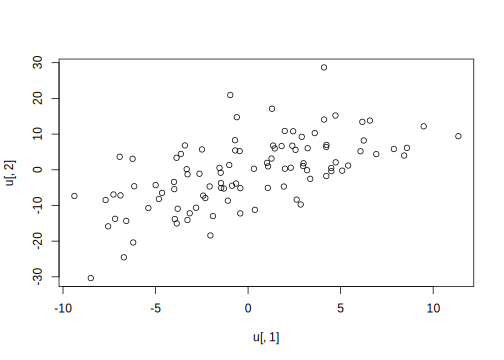
\includegraphics{Freq_CogSci_files/figure-latex/unnamed-chunk-13-1.pdf}

As an exercise, try changing the correlation to \(0\) or to \(-0.6\), and then plot the bivariate distribution that results.

One final useful thing to notice about the variance-covariance matrix is that it can be decomposed into the component standard deviations and an underlying correlation matrix. For example, consider the matrix above:

\begin{Shaded}
\begin{Highlighting}[]
\NormalTok{Sigma}
\end{Highlighting}
\end{Shaded}

\begin{verbatim}
##      [,1] [,2]
## [1,]   25   30
## [2,]   30  100
\end{verbatim}

One can decompose the matrix as follows. The matrix can be seen as the product of a diagonal matrix of the standard deviations and the correlation matrix:

\begin{Shaded}
\begin{Highlighting}[]
\CommentTok{## sds:}
\NormalTok{(sds<-}\KeywordTok{c}\NormalTok{(}\DecValTok{5}\NormalTok{,}\DecValTok{10}\NormalTok{))}
\end{Highlighting}
\end{Shaded}

\begin{verbatim}
## [1]  5 10
\end{verbatim}

\begin{Shaded}
\begin{Highlighting}[]
\CommentTok{## diagonal matrix:}
\NormalTok{(sd_diag<-}\KeywordTok{diag}\NormalTok{(sds))}
\end{Highlighting}
\end{Shaded}

\begin{verbatim}
##      [,1] [,2]
## [1,]    5    0
## [2,]    0   10
\end{verbatim}

\begin{Shaded}
\begin{Highlighting}[]
\CommentTok{## correlation matrix:}
\NormalTok{(corrmatrix<-}\KeywordTok{matrix}\NormalTok{(}\KeywordTok{c}\NormalTok{(}\DecValTok{1}\NormalTok{,}\FloatTok{0.6}\NormalTok{,}\FloatTok{0.6}\NormalTok{,}\DecValTok{1}\NormalTok{),}\DataTypeTok{ncol=}\DecValTok{2}\NormalTok{))}
\end{Highlighting}
\end{Shaded}

\begin{verbatim}
##      [,1] [,2]
## [1,]  1.0  0.6
## [2,]  0.6  1.0
\end{verbatim}

Given these two matrices, one can reassemble the variance-covariance matrix:

\begin{Shaded}
\begin{Highlighting}[]
\NormalTok{sd_diag}\OperatorTok\NormalTok{corrmatrix}\OperatorTok\NormalTok{sd_diag                   }
\end{Highlighting}
\end{Shaded}

\begin{verbatim}
##      [,1] [,2]
## [1,]   25   30
## [2,]   30  100
\end{verbatim}

There is a built-in convenience function, \texttt{sdcor2cov} in the \texttt{SIN} package that does this calculation, taking the vector of standard deviations (not the diagonal matrix) and the correlation matrix to yield the variance-covariance matrix:

\begin{Shaded}
\begin{Highlighting}[]
\NormalTok{SIN}\OperatorTok{::}\KeywordTok{sdcor2cov}\NormalTok{(}\DataTypeTok{stddev=}\NormalTok{sds,}\DataTypeTok{corr=}\NormalTok{corrmatrix)}
\end{Highlighting}
\end{Shaded}

\begin{verbatim}
##      [,1] [,2]
## [1,]   25   30
## [2,]   30  100
\end{verbatim}

We will be using this function a lot when simulating data from hierarchical models.

\hypertarget{likelihood-and-maximum-likelihood-estimation}{%
\section{Likelihood and maximum likelihood estimation}\label{likelihood-and-maximum-likelihood-estimation}}

We now turn to an important topic: the idea of likelihood, and of maximum likelihood estimation. Consider as a first example the discrete case, using the Binomial distribution.

Suppose we toss a fair coin 10 times, and count the number of heads; we do this experiment once. Notice below that we set the probability of success to be 0.5. This is because we are assuming that we tossed a fair coin.

\begin{Shaded}
\begin{Highlighting}[]
\NormalTok{(x<-}\KeywordTok{rbinom}\NormalTok{(}\DecValTok{1}\NormalTok{,}\DataTypeTok{size=}\DecValTok{10}\NormalTok{,}\DataTypeTok{prob=}\FloatTok{0.5}\NormalTok{))}
\end{Highlighting}
\end{Shaded}

\begin{verbatim}
## [1] 3
\end{verbatim}

The \emph{probability} of obtaining this value depends on the parameter we set for \(\theta\) in the PMF for the binomial distribution. Here are some possible values for \(\theta\) and the resulting probabilities:

\begin{Shaded}
\begin{Highlighting}[]
\KeywordTok{dbinom}\NormalTok{(x,}\DataTypeTok{size=}\DecValTok{10}\NormalTok{,}\DataTypeTok{prob=}\FloatTok{0.1}\NormalTok{)}
\end{Highlighting}
\end{Shaded}

\begin{verbatim}
## [1] 0.0574
\end{verbatim}

\begin{Shaded}
\begin{Highlighting}[]
\KeywordTok{dbinom}\NormalTok{(x,}\DataTypeTok{size=}\DecValTok{10}\NormalTok{,}\DataTypeTok{prob=}\FloatTok{0.3}\NormalTok{)}
\end{Highlighting}
\end{Shaded}

\begin{verbatim}
## [1] 0.2668
\end{verbatim}

\begin{Shaded}
\begin{Highlighting}[]
\KeywordTok{dbinom}\NormalTok{(x,}\DataTypeTok{size=}\DecValTok{10}\NormalTok{,}\DataTypeTok{prob=}\FloatTok{0.5}\NormalTok{)}
\end{Highlighting}
\end{Shaded}

\begin{verbatim}
## [1] 0.1172
\end{verbatim}

\begin{Shaded}
\begin{Highlighting}[]
\KeywordTok{dbinom}\NormalTok{(x,}\DataTypeTok{size=}\DecValTok{10}\NormalTok{,}\DataTypeTok{prob=}\FloatTok{0.8}\NormalTok{)}
\end{Highlighting}
\end{Shaded}

\begin{verbatim}
## [1] 0.0007864
\end{verbatim}

\begin{Shaded}
\begin{Highlighting}[]
\KeywordTok{dbinom}\NormalTok{(x,}\DataTypeTok{size=}\DecValTok{10}\NormalTok{,}\DataTypeTok{prob=}\FloatTok{1.0}\NormalTok{)}
\end{Highlighting}
\end{Shaded}

\begin{verbatim}
## [1] 0
\end{verbatim}

The value of \(\theta\) that gives us the highest probability will be called the \textbf{maximum likelihood estimate}. The function \texttt{dbinom} (which is a function of \(\theta\)) is also called a likelihood function, and the maximum value of this function is called the maximum likelihood estimate. We can graphically figure out the maximal value of the \texttt{dbinom} likelihood function here by plotting the value of the function for all possible values of \(\theta\), and checking which is the maximal value:

\begin{Shaded}
\begin{Highlighting}[]
\NormalTok{theta<-}\KeywordTok{seq}\NormalTok{(}\DecValTok{0}\NormalTok{,}\DecValTok{1}\NormalTok{,}\DataTypeTok{by=}\FloatTok{0.01}\NormalTok{)}
\KeywordTok{plot}\NormalTok{(theta,}\KeywordTok{dbinom}\NormalTok{(x,}\DataTypeTok{size=}\DecValTok{10}\NormalTok{,}\DataTypeTok{prob=}\NormalTok{theta),}\DataTypeTok{type=}\StringTok{"l"}\NormalTok{,}
     \DataTypeTok{ylab=}\StringTok{"likelihood/probability"}\NormalTok{)}
\KeywordTok{abline}\NormalTok{(}\DataTypeTok{v=}\NormalTok{x}\OperatorTok{/}\DecValTok{10}\NormalTok{)}
\end{Highlighting}
\end{Shaded}

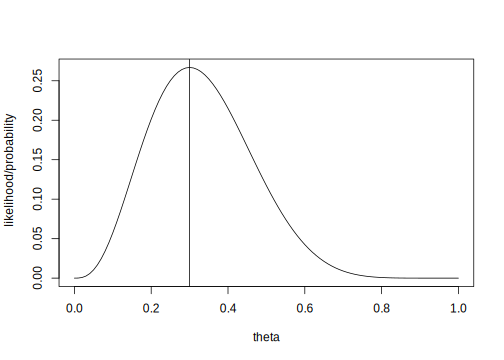
\includegraphics{Freq_CogSci_files/figure-latex/unnamed-chunk-20-1.pdf}

It should be clear from the figure that the maximum value corresponds to the proportion of heads: 3/10. This value is called the maximum likelihood estimate (MLE). We can obtain this MLE of \(\theta\), which maximizes the likelihood, by computing:

\begin{equation}
\hat \theta = \frac{x}{n}
\end{equation}

where \(n\) is sample size, and \(x\) is the number of successes. For the analytical derivation of this result, see the Linear Modeling lecture notes:
\url{https://github.com/vasishth/LM}

The likelihood function in a continuous case is similar to that of the discrete example above, but there is one crucial difference, which we will just get to below.

Consider the following example. Suppose we have one data point from a Normal distribution, with mean 0 and standard deviation 1:

\begin{Shaded}
\begin{Highlighting}[]
\NormalTok{(x<-}\KeywordTok{rnorm}\NormalTok{(}\DecValTok{1}\NormalTok{,}\DataTypeTok{mean=}\DecValTok{0}\NormalTok{,}\DataTypeTok{sd=}\DecValTok{1}\NormalTok{))}
\end{Highlighting}
\end{Shaded}

\begin{verbatim}
## [1] 0.948
\end{verbatim}

The likelihood function for this data point is going to depend on two parameters, \(\mu\) and \(\sigma\). For simplicity, let's assume that \(\sigma\) is known to be 1 and that only \(\mu\) is unknown. In this situation, the value of \(\mu\) that maximizes the likelihood will be the MLE. As before, we can graphically find the MLE by plotting the likelihood function:

\begin{Shaded}
\begin{Highlighting}[]
\NormalTok{mu<-}\KeywordTok{seq}\NormalTok{(}\OperatorTok{-}\DecValTok{3}\NormalTok{,}\DecValTok{3}\NormalTok{,}\DataTypeTok{by=}\FloatTok{0.01}\NormalTok{)}
\KeywordTok{plot}\NormalTok{(mu,}\KeywordTok{dnorm}\NormalTok{(x,}\DataTypeTok{mean=}\NormalTok{mu,}
              \DataTypeTok{sd=}\DecValTok{1}\NormalTok{),}\DataTypeTok{type=}\StringTok{"l"}\NormalTok{)}
\KeywordTok{abline}\NormalTok{(}\DataTypeTok{v=}\NormalTok{x)}
\end{Highlighting}
\end{Shaded}

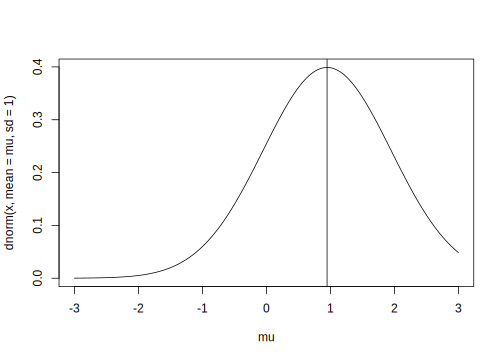
\includegraphics{Freq_CogSci_files/figure-latex/unnamed-chunk-22-1.pdf}

The maximum point in this function will always be the sample mean from the data; the sample mean is the MLE. In the above case, the mean of the single data point 0.948 is the number itself. If we had two data points from a Normal(0,1) distribution, then the likelihood function would be defined as follows. First, let us simulate two data points:

\begin{Shaded}
\begin{Highlighting}[]
\NormalTok{(x1<-}\KeywordTok{rnorm}\NormalTok{(}\DecValTok{1}\NormalTok{))}
\end{Highlighting}
\end{Shaded}

\begin{verbatim}
## [1] -1.202
\end{verbatim}

\begin{Shaded}
\begin{Highlighting}[]
\NormalTok{(x2<-}\KeywordTok{rnorm}\NormalTok{(}\DecValTok{1}\NormalTok{))}
\end{Highlighting}
\end{Shaded}

\begin{verbatim}
## [1] -0.4661
\end{verbatim}

These two data points are independent of each other. Hence, to obtain the joint likelihood, we will have to multiply the likelihoods of each of the numbers, given some value for \(\mu\):

\begin{Shaded}
\begin{Highlighting}[]
\NormalTok{mu<-}\DecValTok{1}
\KeywordTok{dnorm}\NormalTok{(x1,}\DataTypeTok{mean=}\NormalTok{mu)}\OperatorTok{*}\KeywordTok{dnorm}\NormalTok{(x2,}\DataTypeTok{mean=}\NormalTok{mu)}
\end{Highlighting}
\end{Shaded}

In order to plot the joint likelihood, we need to write a function:

\begin{Shaded}
\begin{Highlighting}[]
\NormalTok{normallik<-}\ControlFlowTok{function}\NormalTok{(}\DataTypeTok{mu=}\OtherTok{NULL}\NormalTok{)\{}
  \KeywordTok{dnorm}\NormalTok{(x1,}\DataTypeTok{mean=}\NormalTok{mu)}\OperatorTok{*}\KeywordTok{dnorm}\NormalTok{(x2,}\DataTypeTok{mean=}\NormalTok{mu)}
\NormalTok{\}}
\CommentTok{## test:}
\KeywordTok{normallik}\NormalTok{(}\DataTypeTok{mu=}\DecValTok{1}\NormalTok{)}
\end{Highlighting}
\end{Shaded}

\begin{verbatim}
## [1] 0.004815
\end{verbatim}

Now, we can plot the likelihood function for these two data points:

\begin{Shaded}
\begin{Highlighting}[]
\NormalTok{mu<-}\KeywordTok{seq}\NormalTok{(}\OperatorTok{-}\DecValTok{3}\NormalTok{,}\DecValTok{3}\NormalTok{,}\DataTypeTok{by=}\FloatTok{0.01}\NormalTok{)}
\KeywordTok{plot}\NormalTok{(mu,}\KeywordTok{normallik}\NormalTok{(mu),}\DataTypeTok{type=}\StringTok{"l"}\NormalTok{)}
\KeywordTok{abline}\NormalTok{(}\DataTypeTok{v=}\KeywordTok{mean}\NormalTok{(}\KeywordTok{c}\NormalTok{(x1,x2)))}
\end{Highlighting}
\end{Shaded}

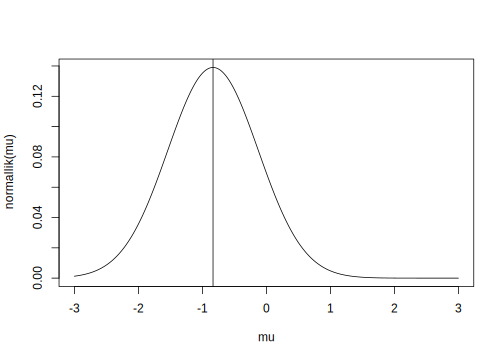
\includegraphics{Freq_CogSci_files/figure-latex/unnamed-chunk-26-1.pdf}

Notice that the maximum value of this joint likelihood is the mean of the two data points.

For the normal distribution, where \(Y \sim N(\mu,\sigma)\), we can get MLEs of \(\mu\) and \(\sigma\) by computing:

\begin{equation}
  \hat \mu = \frac{1}{n}\sum y_i = \bar{y}  
\end{equation}

and

\begin{equation}
    \hat \sigma ^2 = \frac{1}{n}\sum (y_i-\bar{y})^2
\end{equation}

As mentioned earlier, as the formula for the variance, you will sometimes see the unbiased estimate (and this is what R computes) but for large sample sizes the difference is not important:

\begin{equation}
  \hat \sigma ^2 = \frac{1}{n-1}\sum (y_i-\bar{y})^2
\end{equation}

Now we come to a crucial difference between the discrete and continuous cases discussed above. The \texttt{dbinom} is the PMF, but it is also a likelihood function when seen as a function of \(\theta\). Once we have fixed the \(\theta\) parameter to a particular value, the \texttt{dbinom} function gives us the \emph{probability} of a particular outcome.
Given some data \(k\) from \(n\) trials from a Binomial distribution, and treating \(\theta\) as variable between 0 and 1, \texttt{dbinom} gives us the likelihood.

The situation is slightly different in the continuous PDF. Taking the normal distribution as an example, the \texttt{dnorm} function \(f(y|\mu,\sigma)\) doesn't give us the \textbf{probability} of a point value, but rather the \textbf{density}. When the function \(f(y|\mu,\sigma)\) is treated as a function of the parameters, it gives us the \textbf{likelihood}. We need to make a careful distinction between the words probability and likelihood; in day-to-day usage the two words are used interchangeably, but here these two terms have different technical meanings.

A final point to note is that a likelihood function is not a PDF; the area under the curve does not need to sum to 1. By contrast, in a PDF, the area under the curve must sum to 1.

\hypertarget{the-importance-of-the-mle}{%
\subsection{The importance of the MLE}\label{the-importance-of-the-mle}}

One significance of the MLE is that, having assumed a particular underlying PMF/PDF, we can estimate the (unknown) parameters (the mean and variance) of the distribution that we assume to have generated our particular data. For example, in the Binomial case, we have a formula for computing the MLEs of the mean and variance; for the Normal distribution, we have a formula for computing the MLE of the mean and the variance.

What are the distributional properties of the mean \textbf{under repeated sampling}? This is a question that forms the basis for hypothesis testing in the frequentist paradigm. So we turn to this topic in the next chapter.

\hypertarget{summary-of-useful-r-functions-relating-to-univariate-distributions}{%
\section{Summary of useful R functions relating to univariate distributions}\label{summary-of-useful-r-functions-relating-to-univariate-distributions}}

Table \ref{tab:dpqrfunctions} summarizes the different functions relating to univariate PMFs and PDFs, using the Binomial and Normal as examples.

\begin{longtable}[]{@{}lcc@{}}
\caption{\label{tab:dpqrfunctions} Important R functions relating to two univariate distributions, the Binomial and the Normal. In the table, prob represents probability and ranges from 0 to 1. \(P(y)\) is the probability of observing \(y\); \(F(y)\) is the cumulative distribution function (CDF); and \(F^{-1}(prob)\) is the inverse of the CDF.}\tabularnewline
\toprule
& Discrete & Continuous\tabularnewline
\midrule
\endfirsthead
\toprule
& Discrete & Continuous\tabularnewline
\midrule
\endhead
Example: & Binomial(n,\(\theta\)) & Normal(\(\mu,\sigma\))\tabularnewline
Likelihood function & dbinom & dnorm\tabularnewline
Probability: \(P(Y=y)\) & dbinom & always 0\tabularnewline
CDF, \(F(y)=P(Y\geq y)=prob\) & pbinom & pnorm\tabularnewline
Inverse CDF, \(F^{-1}(prob)=y\) & qbinom & qnorm\tabularnewline
Generate simulated data & rbinom & rnorm\tabularnewline
\bottomrule
\end{longtable}

Other distributions, such as the t-distribution, the Uniform, Exponential, Gamma, Beta, etc., have their own set of d-p-q-r functions in R.

\hypertarget{summary-of-random-variable-theory}{%
\section{Summary of random variable theory}\label{summary-of-random-variable-theory}}

We can summarize the above informal concepts relating to random variables very compactly if we re-state them in mathematical form. A mathematical statement has the advantage not only of brevity but also of reducing ambiguity.

Formally, a random variable \(Y\) is defined as a function from a sample space of possible outcomes \(S\) to the real number system:

\begin{equation}
Y : S \rightarrow \mathbb{R}
\end{equation}

The random variable associates to each outcome \(\omega \in S\) exactly one number \(Y(\omega) = y\). \(S_Y\) is all the \(y\)'s (all the possible values of \(Y\), the support of \(Y\)). I.e., \(y \in S_Y\).

Every random variable \(Y\) has associated with it a probability mass (distribution) function (PMF, PDF). I.e., PMF is used for discrete distributions and PDF for continuous distributions. The PMF maps every element of \(S_Y\) to a value between 0 and 1. The PDF maps a range of values in the support of \(Y\) to a value between 0 and 1 (e.g., \(P(a \leq Y\leq b) \rightarrow [0, 1]\)).

\begin{equation}
p_Y : S_Y \rightarrow [0, 1] 
\end{equation}

Probability mass functions (discrete case) and probability density functions (continuous case) are functions that assign probabilities or relative frequencies to events in a sample space.

The expression

\begin{equation}
 Y \sim f(\cdot)
\end{equation}

\noindent
will be used to mean that the random variable \(Y\) has PDF/PMF \(f(\cdot)\).
For example, if we say that \(Y \sim Binomial(n,\theta)\), then we are asserting that the PMF is:

\begin{equation}
\hbox{Binomial}(k|n,\theta) = 
\binom{n}{k} \theta^{k} (1-\theta)^{n-k}
\end{equation}

If we say that \(Y\sim Normal(\mu,\sigma)\), we are asserting that the PDF is

\begin{equation}
Normal(y|\mu,\sigma)= \frac{1}{\sqrt{2\pi \sigma^2}} \exp \left(-\frac{y-\mu)^2}{2\sigma^2} \right)
\end{equation}

The \textbf{cumulative distribution function} or CDF is defined as follows:

For discrete distributions, the probability that \(Y\) is less than \(a\) is written:

\begin{equation}
P(Y<a) = F(Y<a) =\sum_{-\infty}^{a} f(y)
\end{equation}

For continuous distributions, the summation symbol \(\sum\) above becomes the summation symbol for the continuous case, which is the integral \(\int\). The upper and lower bounds are marked by adding a subscript and a superscript on the integral. For example, if we want the area under the curve between points a and b for some function \(f(y)\), we write \(\int_b^a f(y)\, dy\). So, if we want the probability that \(Y\) is less than \(a\), we would write:

\begin{equation}
P(Y<a) = F(Y<a) =\int_{-\infty}^{a} f(y)\, dy
\end{equation}

The above integral is simply summing up the area under the curve between the points \(-\infty\) and \(a\); this gives us the probability of observing \(a\) or a value smaller than \(a\).

We can use the complementary cumulative distribution function to compute quantities like \(P(Y>a)\) by computing \(1-F(a)\), and the quantity \(P(a\leq Y\leq b)\) by computing \(F(b)-F(a)\), where \(b>a\).

A final point here is that we can go back and forth between the PDF and the CDF. If the PDF is \(f(y)\), then the CDF that allows us to compute quantities like \(P(Y<b)\) is just the integral:

\begin{equation}
F(Y<b)=\int_{-\infty}^b f(y)\, dy
\end{equation}

The above is simply computing the area under the curve \(f(y)\), ranging from \(b\) to \(-\infty\).

Because differentiation is the opposite of integration (this is called the Fundamental Theorem of Calculus), if we differentiate the CDF, we get the PDF back:

\begin{equation}
d(F(y))/dy=f(y)
\end{equation}

In bivariate distributions, the joint CDF is written \(F_{X,Y}(a,b)=P(X\leq a, Y\leq b)\), where \(-\infty < a,b<\infty\). The \emph{marginal distributions} of \(F_X\) and \(F_Y\) are the CDFs of each of the associated random variables. The CDF of \(X\):

\begin{equation}
F_X(a) = P(X\leq a) = F_X(a,\infty) 
\end{equation}

The CDF of \(Y\):

\begin{equation}
F_Y(b) = P(Y\leq b) = F_Y(\infty,b) 
\end{equation}

\(f(x,y)\) is the \emph{joint PDF} of \(X\) and \(Y\). Every joint PDF satisfies

\begin{equation}
f(x,y)\geq 0\mbox{ for all }(x,y)\in S_{X,Y},
\end{equation}
and
\begin{equation}
\int \int_{S_{X,Y}}f(x,y)\,\mathrm{d} x\,\mathrm{d} y=1.
\end{equation}

where \(S_{X,Y}\) is the joint support of the two random variables.

If X and Y are jointly continuous, they are individually continuous, and their PDFs are:

\begin{equation}
\begin{split}
P(X\in A) = & P(X\in A, Y\in (-\infty,\infty))  \\
= & \int_A \int_{-\infty}^{\infty} f(x,y)\,dy\, dx\\
= & \int_A f_X(x)\, dx
\end{split} 
\end{equation}

\noindent
where

\begin{equation}
f_X(x) = \int_{-\infty}^{\infty} f(x,y)\, dy    
\end{equation}

Similarly:

\begin{equation}
f_Y(y) =  \int_{-\infty}^{\infty} f(x,y)\, dx       
\end{equation}

\hypertarget{further-reading}{%
\section{Further reading}\label{further-reading}}

For readers interested in the mathematics needed for statistics, the books by \citet{fox2009mathematical}, \citet{gill2006essential}, and \citet{moore2013mathematics} are useful. The essential matrix algebra needed for statistics is discussed in \citet{fieller}. Accessible introductions to probability theory are \citet{morin2016probability} and \citet{blitzstein2014introduction}. \citet{kerns} contains a very well-written and freely available general introduction to random variable theory and statistics, but assumes the reader knows the basics of calculus.

\hypertarget{sec:Foundationsexercises}{%
\section{Exercises}\label{sec:Foundationsexercises}}

\hypertarget{sec:Foundationsexercisespnorm}{%
\subsection{\texorpdfstring{Practice using the \texttt{pnorm} function}{Practice using the pnorm function}}\label{sec:Foundationsexercisespnorm}}

\hypertarget{sec:FoundationsexercisespnormPart1}{%
\subsubsection{Part 1}\label{sec:FoundationsexercisespnormPart1}}

Given a normal distribution with mean \texttt{57} and standard deviation \texttt{100}, use the pnorm function to calculate the probability of obtaining values between \texttt{222} and \texttt{84} from this distribution.

\hypertarget{sec:FoundationsexercisespnormPart2}{%
\subsubsection{Part 2}\label{sec:FoundationsexercisespnormPart2}}

Calculate the following probabilities.
Given a normal distribution with mean \texttt{51} and standard deviation \texttt{4}, what is the probability of getting

\begin{itemize}
\tightlist
\item
  a score of \texttt{41} or less
\item
  a score of \texttt{41} or more
\item
  a score of \texttt{54} or more
\end{itemize}

\hypertarget{sec:FoundationsexercisespnormPart3}{%
\subsubsection{Part 3}\label{sec:FoundationsexercisespnormPart3}}

Given a normal distribution with mean \texttt{51} and standard deviation \texttt{7}, what is the probability of getting

\begin{itemize}
\tightlist
\item
  a score of \texttt{46} or less.
\item
  a score between \texttt{48} and \texttt{54}.
\item
  a score of \texttt{mu+1} or more.
\end{itemize}

\hypertarget{sec:Foundationsexercisesqnorm}{%
\subsection{\texorpdfstring{Practice using the \texttt{qnorm} function}{Practice using the qnorm function}}\label{sec:Foundationsexercisesqnorm}}

\hypertarget{sec:FoundationsexercisesqnormPart1}{%
\subsubsection{Part 1}\label{sec:FoundationsexercisesqnormPart1}}

Consider a normal distribution with mean 1 and standard deviation 1.

Compute the lower and upper boundaries such that:

\begin{itemize}
\tightlist
\item
  the area (the probability) to the left of the lower boundary is \texttt{0.37}.
\item
  the area (the probability) to the left of the upper boundary is \texttt{0.94}.
\end{itemize}

\hypertarget{sec:FoundationsexercisesqnormPart2}{%
\subsubsection{Part 2}\label{sec:FoundationsexercisesqnormPart2}}

Given a normal distribution with mean \texttt{50.643} and standard deviation \texttt{0.736}. There exist two quantiles, the lower quantile q1 and the upper quantile q2, that are equidistant from the mean \texttt{50.643}, such that the area under the curve of the Normal probability between q1 and q2 is \texttt{85}\%. Find q1 and q2.

\hypertarget{sec:FoundationsexercisesMLE1}{%
\subsection{Maximum likelihood estimation 1}\label{sec:FoundationsexercisesMLE1}}

The function \texttt{dnorm} gives the likelihood given a data point (or multiple data) and a value for the mean and the standard deviation (sd). Using \texttt{dnorm}, compute

\begin{itemize}
\tightlist
\item
  the likelihood of the data point \texttt{11.664} assuming a mean of \texttt{12} and standard deviation 5.
\item
  the likelihood of the data point \texttt{11.664} assuming a mean of \texttt{11} and standard deviation 5.
\item
  the likelihood of the data point \texttt{11.664} assuming a mean of \texttt{10} and standard deviation 5.
\item
  the likelihood of the data point \texttt{11.664} assuming a mean of \texttt{9} and standard deviation 5.
\end{itemize}

\hypertarget{sec:FoundationsexercisesMLE2}{%
\subsection{Maximum likelihood estimation 2}\label{sec:FoundationsexercisesMLE2}}

You are given \(10\) independent and identically distributed data points that are assumed to come from a Normal distribution with unknown mean and unknown standard deviation:

\begin{Shaded}
\begin{Highlighting}[]
\NormalTok{x}
\end{Highlighting}
\end{Shaded}

\begin{verbatim}
##  [1] 503 487 511 488 516 501 488 484 493 505
\end{verbatim}

The function \texttt{dnorm} gives the likelihood given multiple data points and a value for the mean and the standard deviation. The log-likelihood can be computed by typing \texttt{dnorm(...,log=TRUE)}.

The product of the likelihoods for two independent data points can be computed like this: Suppose we have two independent and identically distributed data points 5 and 10. Then, assuming that the Normal distribution they come from has mean 10 and standard deviation 2, the joint likelihood of these is:

\begin{Shaded}
\begin{Highlighting}[]
\KeywordTok{dnorm}\NormalTok{(}\DecValTok{5}\NormalTok{,}\DataTypeTok{mean=}\DecValTok{10}\NormalTok{,}\DataTypeTok{sd=}\DecValTok{2}\NormalTok{)}\OperatorTok{*}\KeywordTok{dnorm}\NormalTok{(}\DecValTok{10}\NormalTok{,}\DataTypeTok{mean=}\DecValTok{10}\NormalTok{,}\DataTypeTok{sd=}\DecValTok{2}\NormalTok{)}
\end{Highlighting}
\end{Shaded}

\begin{verbatim}
## [1] 0.001748
\end{verbatim}

It is easier to do this on the log scale, because then one can add instead of multiplying. This is because \(\log(x\times y)= \log(x) + \log(y)\). For example:

\begin{Shaded}
\begin{Highlighting}[]
\KeywordTok{log}\NormalTok{(}\DecValTok{2}\OperatorTok{*}\DecValTok{3}\NormalTok{)}
\end{Highlighting}
\end{Shaded}

\begin{verbatim}
## [1] 1.792
\end{verbatim}

\begin{Shaded}
\begin{Highlighting}[]
\KeywordTok{log}\NormalTok{(}\DecValTok{2}\NormalTok{) }\OperatorTok{+}\StringTok{ }\KeywordTok{log}\NormalTok{(}\DecValTok{3}\NormalTok{)}
\end{Highlighting}
\end{Shaded}

\begin{verbatim}
## [1] 1.792
\end{verbatim}

So the joint log likelihood of the two data points is:

\begin{Shaded}
\begin{Highlighting}[]
\KeywordTok{dnorm}\NormalTok{(}\DecValTok{5}\NormalTok{,}\DataTypeTok{mean=}\DecValTok{10}\NormalTok{,}\DataTypeTok{sd=}\DecValTok{2}\NormalTok{,}\DataTypeTok{log=}\OtherTok{TRUE}\NormalTok{)}\OperatorTok{+}\KeywordTok{dnorm}\NormalTok{(}\DecValTok{10}\NormalTok{,}\DataTypeTok{mean=}\DecValTok{10}\NormalTok{,}\DataTypeTok{sd=}\DecValTok{2}\NormalTok{,}\DataTypeTok{log=}\OtherTok{TRUE}\NormalTok{)}
\end{Highlighting}
\end{Shaded}

\begin{verbatim}
## [1] -6.349
\end{verbatim}

Even more compactly:

\begin{Shaded}
\begin{Highlighting}[]
\KeywordTok{sum}\NormalTok{(}\KeywordTok{dnorm}\NormalTok{(}\KeywordTok{c}\NormalTok{(}\DecValTok{5}\NormalTok{,}\DecValTok{10}\NormalTok{),}\DataTypeTok{mean=}\DecValTok{10}\NormalTok{,}\DataTypeTok{sd=}\DecValTok{2}\NormalTok{,}\DataTypeTok{log=}\OtherTok{TRUE}\NormalTok{))}
\end{Highlighting}
\end{Shaded}

\begin{verbatim}
## [1] -6.349
\end{verbatim}

\begin{itemize}
\tightlist
\item
  Given the 10 data points above, calculate the maximum likelihood estimate (MLE) of the expectation.
\item
  The sum of the log-likelihoods of the data x, using as the mean the MLE from the sample, and standard deviation 5.
\item
  What is the sum of the log-likelihood if the mean used to compute the log-likelihood is \texttt{495.6}?
\item
  Which value for the mean, the MLE or \texttt{495.6}, gives the higher log-likelihood?
\end{itemize}

\hypertarget{sec:Foundationsexercisesbivar}{%
\subsection{Generating bivariate data}\label{sec:Foundationsexercisesbivar}}

Generate 50 data points from two random variables X and Y, where \(X\sim Normal(50,100)\) and \(Y\sim Normal(100,20)\). The correlation between the random variables is 0.7. Plot the simulated data points from Y against those from X.

\hypertarget{sec:Foundationsexercisesmultivar}{%
\subsection{Generating multivariate data}\label{sec:Foundationsexercisesmultivar}}

The bivariate case can be generalized to more than two dimensions.
Generate 50 data points from three random variables X, Y, and Z, where \(X\sim Normal(50,100)\), \(Y\sim Normal(100,20)\), and \(Z\sim Normal(200,50)\). The correlation between the random variables X and Y is 0.5, between X and Z is 0.2, an between Y and Z is 0.7. Here, you will have to define a \(3\times 3\) variance covariance matrix, with the pairwise covariances in the off-diagonals. Plot the simulated data points as two-dimensional figures: Y against X, Y against Z, and X against Z.

\hypertarget{hypothetical-repeated-sampling-and-the-t-test}{%
\chapter{Hypothetical repeated sampling and the t-test}\label{hypothetical-repeated-sampling-and-the-t-test}}

This chapter introduces some of the foundational ideas behind hypothesis testing in the frequentist framework. The key idea is that of hypothetical repeated sampling. When we fit a model to a given data-set, we are assuming that this is one of potentially infinite numbers of exact repetitions of an experiment. We will leverage some amazing properties of these exact repetitions in order to draw inferences from our particular data. The key idea to understand here is the central limit theorem, which we will discuss below. Before we do that, it is useful to introduce some terminology relating to typical experiment designs in linguistics and psychology.

\hypertarget{some-terminology-surrounding-typical-experiment-designs-in-linguistics-and-psychology}{%
\section{Some terminology surrounding typical experiment designs in linguistics and psychology}\label{some-terminology-surrounding-typical-experiment-designs-in-linguistics-and-psychology}}

An experiment typically involves taking a \emph{random sample} from some population. For example, we could take a sample of participants and record their reading times for two types of sentences, for example easy and difficult sentences. How one operationalizes easy and difficult is not important at this point. However, to make the discussion concrete, consider this well-known example from psycholinguistics. We could be comparing reading times in active vs.~passive sentences:

Active sentence: The man threw the ball.

Passive sentence: The ball was thrown by the man.

One claim in the literature is that, due to their simpler structure, active sentences are easier to process than passive sentences. So this is an example of a simpler vs.~complex sentence. If we want to investigate whether actives are easier to process than passives, we can, as an example, compare the total reading times for each sentence type (there are some problems that arise here because the sentences don't have the same length, so the comparison is not really fair; these issues we will discuss later).

Technically, we are supposed to randomly choose participants; in practice, this randomization rarely happens. Instead we take whatever participants we get, such as university students who happen to apply to participate in an experiment! So, random sampling is an assumption in all the discussions in this chapter, but in practice this assumption may or may not be perfectly met.

One design decision that the researcher must take is whether to collect only one response from each participant in each condition, or whether we collect multiple measures from each participant. If we collect only one data point from each participant, we will say that the data points are \emph{independent} of each other. When we collect multiple measurements from each participant, we will say that we have \emph{dependent} data; such multiple measurements are also called \emph{repeated measures}. With repeated measures, there will be some correlation between the data-points because the multiple measurements from a common source.

In psycholinguistics, repeated measures experiments are the norm. Furthermore, it is common to use a so-called \emph{Latin Square} design. To understand this design, suppose we want to conduct an experiment with two conditions, a and b, and that we want each participant to see each condition multiple times (repeated measurements). The way such an experiment (with two conditions) is set up with a Latin Square design is that we would create multiple pairs of items, e.g., items 1a, 1b, 2a, 2b, etc. For example, we are investigating active vs.~passive sentences, item 1a could be the active clause \emph{The man threw the ball}, and 1b would thene the passive counterpart \emph{The ball was thrown by the man}. The two versions of the item are therefore minimal pairs---minimally different in that the sentence has the same words, but one is an active clause and the other a passive clause.

Then, we would create two groups of items, G1 and G2. Group G1 would contain items 1a, 2b, 3a, 4b, etc; group G2 would contain items 1b, 2a, 3b, 4a, etc. Thus, if one had 16 items, each group would contain eight instance of each condition. Having set up these two groups, one would then randomly assign each participant to one of the two groups. In this way, from each participant, we would obtain eight repeated measures from each condition. One can (and should) of course randomize the order of presentation in each group, possibly randomizing afresh for each participant. The term Latin Square refers to the fact that the ordering of the conditions forms a square.

\begin{longtable}[]{@{}l@{}}
\toprule
\endhead
\textbar{} a \textbar{} b \textbar{}\tabularnewline
\textbar{} b \textbar{} a \textbar{}\tabularnewline
\bottomrule
\end{longtable}

Each condition appears in each row exactly once.

The Latin square generalizes beyond two conditions easily. Suppose we have four conditions; then, the Latin Square is:

\begin{longtable}[]{@{}l@{}}
\toprule
\endhead
\textbar{} a \textbar{} b \textbar{} c \textbar{} d \textbar{}\tabularnewline
\textbar{} b \textbar{} c \textbar{} d \textbar{} a \textbar{}\tabularnewline
\textbar{} c \textbar{} d \textbar{} a \textbar{} b \textbar{}\tabularnewline
\textbar{} d \textbar{} a \textbar{} b \textbar{} d \textbar{}\tabularnewline
\bottomrule
\end{longtable}

Similarly if you have eight conditions, the Latin Square table would look like this.

\begin{longtable}[]{@{}l@{}}
\toprule
\endhead
\textbar{} a \textbar{} b \textbar{} c \textbar{} d \textbar{} e \textbar{} f \textbar{} g \textbar{} h \textbar{}\tabularnewline
\textbar{} b \textbar{} c \textbar{} d \textbar{} e \textbar{} f \textbar{} g \textbar{} h \textbar{} a \textbar{}\tabularnewline
\textbar{} c \textbar{} d \textbar{} e \textbar{} f \textbar{} g \textbar{} h \textbar{} a \textbar{} b \textbar{}\tabularnewline
\textbar{} d \textbar{} e \textbar{} f \textbar{} g \textbar{} h \textbar{} a \textbar{} b \textbar{} c \textbar{}\tabularnewline
\textbar{} e \textbar{} f \textbar{} g \textbar{} h \textbar{} a \textbar{} b \textbar{} c \textbar{} d \textbar{}\tabularnewline
\textbar{} f \textbar{} g \textbar{} h \textbar{} a \textbar{} b \textbar{} c \textbar{} d \textbar{} e \textbar{}\tabularnewline
\textbar{} g \textbar{} h \textbar{} a \textbar{} b \textbar{} c \textbar{} d \textbar{} e \textbar{} f \textbar{}\tabularnewline
\textbar{} h \textbar{} a \textbar{} b \textbar{} c \textbar{} d \textbar{} e \textbar{} f \textbar{} g \textbar{}\tabularnewline
\bottomrule
\end{longtable}

As an aside, it is rarely a good idea to design such complex experiments! The more conditions you have in an experiment, the more decisions you will have to make about how to analyze the data, and the harder the interpretation of the data. Later in this course, we will demonstrate the price one has to pay for setting up overly complex designs. We mention this point here because it is a common beginner error to want to have as many conditions as possible in a single experiment. In fact, a student of ours once proposed a 180 condition design!

The Latin Square design is attractive for psycholinguistics and psychology because it has some optimality properties. Experiment design and the properties of different designs is a whole field in itself in statistics, but we won't get into these details.

One consequence of the above repeated measurements design is that we have multiple measurements not just from participants but also from items! Thus, items can also be seen as producing dependent data. In other words, both participants and items are producing dependent data in this design. Later on, we will see that this has an effect on the type of data analysis one can do.

With this very brief introduction to experiment design, we now turn to the idea of hypothetical repeated sampling, and the central limit theorem.

\hypertarget{the-central-limit-theorem-using-simulation}{%
\section{The central limit theorem using simulation}\label{the-central-limit-theorem-using-simulation}}

Suppose we collect some data, which can be represented by a vector \(y\); this is a \emph{single sample}. Given data \(y\), and assuming for concreteness that the underlying likelihood is a \(Normal(\mu=500,\sigma=100)\), the sample mean and standard deviation, \(\bar{y}\) and \(s\) give us an estimate of the unknown parameters mean \(\mu\) and the standard deviation \(\sigma\) of the distribution from which we assume that our data come from. Figure \ref{fig:normalsample} shows the distribution of a particular sample, where the number of data points is \(n=1000\). Note that in this example the parameters are specified by us, so they are not unknown; in a real data-collection situation, the sample mean and standard deviation are all we have as estimates of the parameters.

\begin{Shaded}
\begin{Highlighting}[]
\CommentTok{## sample size:}
\NormalTok{n<-}\DecValTok{1000}
\CommentTok{##  independent and identically distributed sample:}
\NormalTok{y<-}\KeywordTok{rnorm}\NormalTok{(n,}\DataTypeTok{mean=}\DecValTok{500}\NormalTok{,}\DataTypeTok{sd=}\DecValTok{100}\NormalTok{)}
\CommentTok{## histogram of data:}
\KeywordTok{hist}\NormalTok{(y,}\DataTypeTok{freq=}\OtherTok{FALSE}\NormalTok{)}
\CommentTok{## true value of mean:}
\KeywordTok{abline}\NormalTok{(}\DataTypeTok{v=}\DecValTok{500}\NormalTok{,}\DataTypeTok{lwd=}\DecValTok{2}\NormalTok{)}
\end{Highlighting}
\end{Shaded}

\begin{figure}
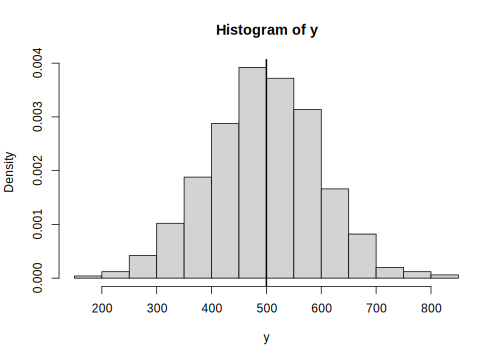
\includegraphics[width=0.75\linewidth]{Freq_CogSci_files/figure-latex/normalsample-1} \caption{A sample of data y of size n=100, from the distribution  Normal(500,100). The vertical line shows the true mean of the distribution we are sampling from.}\label{fig:normalsample}
\end{figure}

Suppose now that you had not a single sample of size 1000 but many repeated samples. This isn't something one can normally do in real life; we often run a single experiment or, at most, repeat the same experiment once. However, one can simulate repeated sampling easily within R. Let us take 100 repeated samples like the one above, and save the samples in a matrix containing n=1000 rows and 100 columns, each column representing an experiment:

\begin{Shaded}
\begin{Highlighting}[]
\NormalTok{mu<-}\DecValTok{500}
\NormalTok{sigma<-}\DecValTok{100}
\CommentTok{## number of experiments:}
\NormalTok{k<-}\DecValTok{100}
\CommentTok{## store for data:}
\NormalTok{y_matrix<-}\KeywordTok{matrix}\NormalTok{(}\KeywordTok{rep}\NormalTok{(}\OtherTok{NA}\NormalTok{,n}\OperatorTok{*}\NormalTok{k),}\DataTypeTok{ncol=}\NormalTok{k)}
\ControlFlowTok{for}\NormalTok{(i }\ControlFlowTok{in} \DecValTok{1}\OperatorTok{:}\NormalTok{k)\{}
  \CommentTok{## expt result with sample size n:}
\NormalTok{  y_matrix[,i]<-}\KeywordTok{rnorm}\NormalTok{(n,}\DataTypeTok{mean=}\NormalTok{mu,}\DataTypeTok{sd=}\NormalTok{sigma)}
\NormalTok{\}}
\end{Highlighting}
\end{Shaded}

Now, if we compute the means \(\bar{y}_k\) of \emph{each} of the \(k=1,\dots,100\) experiments we just carried out, if certain conditions are met, these means will be normally distributed, with mean \(\mu\) and standard deviation \(\sigma/\sqrt{n}\). To understand this point, it is useful to first visualize the distribution of means and graphically summarize this standard deviation, which confusingly is called \emph{standard error}.

\begin{Shaded}
\begin{Highlighting}[]
\CommentTok{## compute means from each replication:}
\NormalTok{y_means<-}\KeywordTok{colMeans}\NormalTok{(y_matrix)}
\CommentTok{## the mean and sd (=standard error) of the means}
\KeywordTok{mean}\NormalTok{(y_means);}\KeywordTok{sd}\NormalTok{(y_means)}
\end{Highlighting}
\end{Shaded}

\begin{verbatim}
## [1] 499.8
\end{verbatim}

\begin{verbatim}
## [1] 3.067
\end{verbatim}

\begin{figure}
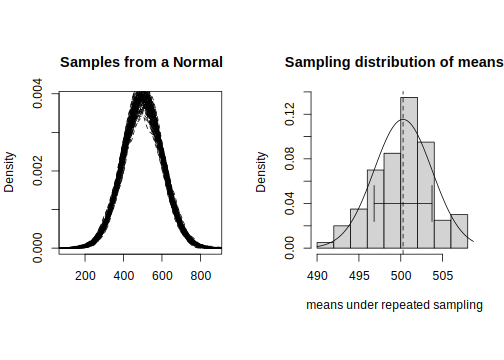
\includegraphics[width=0.75\linewidth]{Freq_CogSci_files/figure-latex/sdsmnormal-1} \caption{Sampling from a normal distribution (left); and the sampling distribution of the means under repeated sampling (right). The right-hand plot shows an overlaid normal distribution, and the standard deviation (standard error) as error bars.}\label{fig:sdsmnormal}
\end{figure}

The sampling distribution of means has a normal distribution provided two conditions are met: (a) the sample size should be ``large enough'', and (b) \(\mu\) and \(\sigma\) are defined for the probability density or mass function that generated the data. This fact is called the \textbf{central limit theorem} (CLT). The significance of the CLT for us as researchers is that from the summary statistics computed from a \emph{single} sample, we can obtain an estimate of this distribution of means: \(Normal(\bar{y},s/\sqrt{n})\).

The statement that the sampling distribution of the means will be normal, with mean \(\mu\) and standard deviation \(\sigma/\sqrt{n}\), can be derived formally through a surprisingly simple application of random variable theory. Suppose we gather independent and identically distributed data \(y_1, \dots, y_n\), each of which is generated by a random variable \(Y\sim Normal(\mu,\sigma)\).

When we compute the mean \(\bar{y}\) for each sample, we are assuming that each of the means is coming from a random variable \(\bar{Y}\), which is just a linear combination of values generated by instances of the random variable \(Y\), which itself has a pdf with mean (expectation) \(\mu\) and variance \(\sigma^2\):

\begin{equation}
\bar{Y}=\frac{1}{n} \sum_{i=1}^n Y = \frac{1}{n}Y_1 + \dots + \frac{1}{n}Y_n
 \end{equation}

So, the expectation of \(\bar{Y}\) is

\begin{equation}
\begin{split}
E[\bar{Y}] =& E[\frac{1}{n}Y_1 + \dots + \frac{1}{n}Y_n]\\
=& \frac{1}{n} (E[Y] + \dots + E[Y])\\
=& \frac{1}{n} (\mu + \dots + \mu)\\
=& \frac{1}{n} n\mu \\
=& \mu \\
\end{split}
\end{equation}

And the variance of \(\bar{Y}\) is

\begin{equation}
\begin{split}
Var(\bar{Y}) =& Var(\frac{1}{n}Y_1 + \dots + \frac{1}{n}
Y_n)\\
=& \frac{1}{n^2} Var(Y_1 + \dots + Y_n)\\
\end{split}
\end{equation}

The last line above arises because the variance of a random variable \(Z\) multiplied by a constant \(a\), \(Var(aZ)\) is \(a^2 Var(Z)\). Here, \(a=1/n\), so \(a^2 = 1/n^2\).
Because \(Y_1,\dots,Y_n\) are independent, we can compute the variance \(Var(Y_1 + \dots + Y_n)\) by using the fact that the variance of the sum of independent random variables is the sum of their variances. This fact gives us:

\begin{equation} \label{sdsmderivation}
\begin{split}
\frac{1}{n^2} Var(Y_1 + \dots + Y_n) =& \frac{1}{n^2} (Var(Y) + \dots + Var(Y))\\
=&  \frac{1}{n^2}  n Var(Y)\\
=&  \frac{1}{n}  Var(Y)\\
=&  \frac{\sigma^2}{n}\\
\end{split}
\end{equation}

This derives the above result that the expectation (i.e., the mean) and variance of the sampling distribution of the sample means are

\begin{equation}
E[\bar{Y}] = \mu \quad Var(\bar{Y}) = \frac{\sigma^2}{n}
\end{equation}

The above means that we can estimate the expectation \(\bar{Y}\) and the variance of \(\bar{Y}\) from a \emph{single} sample!!

The Central Limit Theorem, not proved here (for a proof, see p.~267 of \citet{millermiller}) can be summarized as follows.

\textbf{Central Limit Theorem}

Let \(f(Y)\) be the pdf of a random variable \(Y\), and assume that the pdf has mean \(\mu\) and variance \(\sigma^2\). Then:

\begin{equation}
\bar{Y} \sim Normal(\mu,\sigma^2/n) \quad  E[Y]=\mu,Var(Y)=\sigma^2 \quad \hbox{ when n is large}
\end{equation}

For us, the practical implication of this result is huge. From a \emph{single} sample of \(n\) independent data points \(y_1,\dots, y_n\), we can derive the distribution of \emph{hypothetical} sample means under repeated sampling. That is, it becomes possible to say something about what the plausible and implausible values of the sample mean are under repeated sampling. This is the basis for all hypothesis testing and statistical inference in the frequentist framework that we will look at in this book.

Sometimes the central limit theorem is misunderstood to imply that the pdf \(f(Y)\) that is assumed to generate the data is always going to be normal. It is important to understand that there are two pdfs we are talking about here. First, there is the pdf that the data were generated from; this need not be normal. For example, you could get data from a Normal, Exponential, Gamma, or other distribution. Second, there is the sampling distribution of the \emph{sample mean} under repeated sampling. It is the sampling distribution that the central limit theorem is about, not the distribution that generated the data.

\hypertarget{three-examples-of-the-sampling-distribution}{%
\section{Three examples of the sampling distribution}\label{three-examples-of-the-sampling-distribution}}

In the above discussion, the underlying pdf we sampled from above was a normal distribution. However, it need not be. Consider two examples first: the underlying pdf is an Exponential or a Gamma distribution.

The Exponential distribution has a parameter \(\lambda\) (parameterized in \texttt{R} as a \texttt{rate}, \(1/\lambda\)); its mean is \(\lambda\) and its variance is \(1/\lambda^2\). The sampling distribution is normal, even though the underlying distribution is an Exponential; see Figure \ref{fig:sdsmexp}.

\begin{figure}
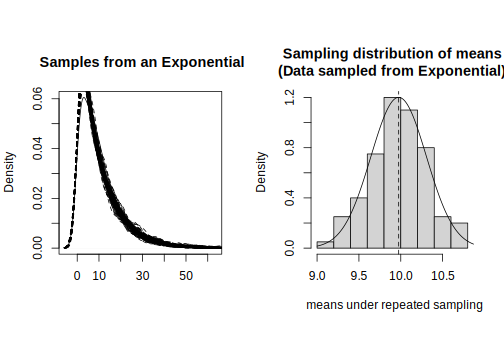
\includegraphics[width=0.85\linewidth]{Freq_CogSci_files/figure-latex/sdsmexp-1} \caption{Sampling from an exponential.}\label{fig:sdsmexp}
\end{figure}

A further example is samples from a Gamma distribution. Suppose we sample from a Gamma distribution with shape parameter chosen arbitrarily to be 1. The distribution of means is again going to be approximately normal; see Figure \ref{fig:sdsmgamma}.

\begin{figure}
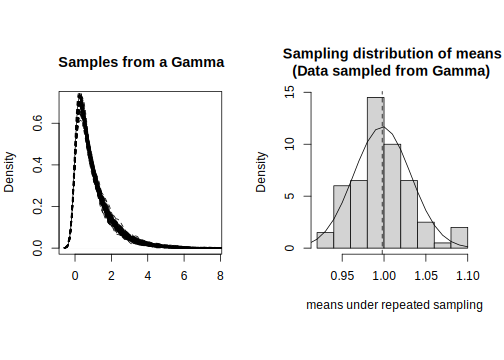
\includegraphics[width=0.75\linewidth]{Freq_CogSci_files/figure-latex/sdsmgamma-1} \caption{Sampling from a Gamma distribution.}\label{fig:sdsmgamma}
\end{figure}

As a final example, consider what happens if sample from a distribution, the Cauchy, that doesn't have any mean or variance defined for it.

\begin{figure}
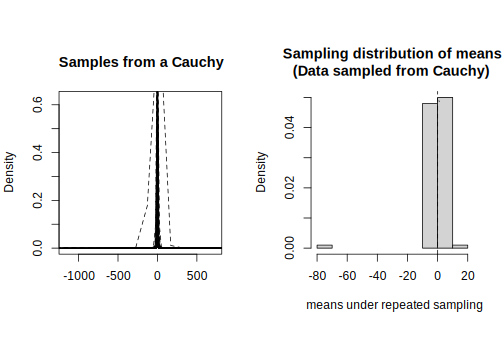
\includegraphics[width=0.75\linewidth]{Freq_CogSci_files/figure-latex/sdsmcauchy-1} \caption{Sampling from a Cauchy distribution.}\label{fig:sdsmcauchy}
\end{figure}

As the Figure @(fig:sdsmcauchy) illustrates, when the mean and variance for the likelihood are undefined, the central limit theorem doesn't hold. In the rest of this book, we will always assume that the data are coming from a distribution that has a mean and variance defined for it.

\hypertarget{the-confidence-interval-and-what-its-good-for}{%
\section{The confidence interval, and what it's good for}\label{the-confidence-interval-and-what-its-good-for}}

Once we have sample of data \(y\), and once the sample mean \(\bar{y}\) and the \(SE = s/\sqrt{n}\) have been computed, it is common to define a so-called 95\% confidence interval:

\begin{equation}
\bar{y} \pm 2 SE
\end{equation}

Because the sampling distribution of means is normally distributed, and because 95\% of the area under the curve is covered by two times the standard deviation of the normal distribution,\\
the upper and lower bounds of the interval defined by the interval \(\bar{y} \pm 2 SE\) covers approximately 95\% of the area under the curve in the sampling distribution.

This interval is usually computed after estimating the sample mean and standard error from a data-set, and is called the \emph{confidence interval} (CI). It has the following meaning: If you take samples repeatedly and compute the CI each time, 95\% of those CIs will contain the true population mean \(\mu\). To understand this point, one can simulate this situation. This time we will do 1000 repeated experiments instead of 100.

\begin{Shaded}
\begin{Highlighting}[]
\NormalTok{mu<-}\DecValTok{500}
\NormalTok{sigma<-}\DecValTok{100}
\NormalTok{n<-}\DecValTok{1000}
\NormalTok{nsim<-}\DecValTok{1000}
\NormalTok{lower<-}\KeywordTok{rep}\NormalTok{(}\OtherTok{NA}\NormalTok{,nsim)}
\NormalTok{upper<-}\KeywordTok{rep}\NormalTok{(}\OtherTok{NA}\NormalTok{,nsim)}
\ControlFlowTok{for}\NormalTok{(i }\ControlFlowTok{in} \DecValTok{1}\OperatorTok{:}\NormalTok{nsim)\{}
\NormalTok{  y<-}\KeywordTok{rnorm}\NormalTok{(n,}\DataTypeTok{mean=}\NormalTok{mu,}\DataTypeTok{sd=}\NormalTok{sigma)}
\NormalTok{  lower[i]<-}\KeywordTok{mean}\NormalTok{(y) }\OperatorTok{-}\StringTok{ }\DecValTok{2} \OperatorTok{*}\StringTok{ }\KeywordTok{sd}\NormalTok{(y)}\OperatorTok{/}\KeywordTok{sqrt}\NormalTok{(n)}
\NormalTok{  upper[i]<-}\KeywordTok{mean}\NormalTok{(y) }\OperatorTok{+}\StringTok{ }\DecValTok{2} \OperatorTok{*}\StringTok{ }\KeywordTok{sd}\NormalTok{(y)}\OperatorTok{/}\KeywordTok{sqrt}\NormalTok{(n)}
\NormalTok{\}}

\CommentTok{## check how many CIs contain mu:}
\NormalTok{CIs<-}\KeywordTok{ifelse}\NormalTok{(lower}\OperatorTok{<}\NormalTok{mu }\OperatorTok{&}\StringTok{ }\NormalTok{upper}\OperatorTok{>}\NormalTok{mu,}\DecValTok{1}\NormalTok{,}\DecValTok{0}\NormalTok{)}
\CommentTok{## approx. 95% of the CIs contain true mean:}
\KeywordTok{round}\NormalTok{(}\KeywordTok{mean}\NormalTok{(CIs),}\DecValTok{2}\NormalTok{)}
\end{Highlighting}
\end{Shaded}

\begin{verbatim}
## [1] 0.96
\end{verbatim}

Figure \ref{fig:ciplot} visualizes the coverage properties of the confidence interval in 100 simulations; by coverage we mean here the proportion of cases where the true \(\mu\) is contained in the CI.

\begin{figure}
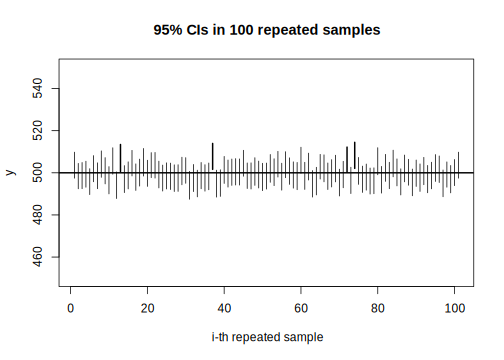
\includegraphics[width=0.75\linewidth]{Freq_CogSci_files/figure-latex/ciplot-1} \caption{Illustration of the meaning of a  95 percent confidence interval (CI). The thicker bars represent the CIs which do not contain the true mean.}\label{fig:ciplot}
\end{figure}

The confidence interval is widely misinterpreted, i.e., as representing the range of plausible value of the \(\mu\) parameter. This is the wrong interpretation because \(\mu\) is a point value by assumption, it doesn't have a pdf associated with it. The frequentist CI is defined with reference to the sampling distribution of the mean under repeated sampling, not the probability distribution of \(\mu\).
By contrast, the Bayesian credible interval does have this interpretation.
In most modeling settings we have encountered in our work, the frequentist confidence interval and Bayesian credible interval have very similar widths, with the Bayesian interval being slightly wider depending on the prior specifications.

Given the convoluted meaning of the CI, and the impossibility of interpreting a single CI, it is reasonable to ask: what good is a CI? One can treat the CI as a summary that tells us the width of the sampling distribution of the mean---the wider the sampling distribution, the more the implied variability under repeated sampling. The confidence interval can therefore be used to assess how uncertain we can be about the estimate of the sample mean under hypothetical repeated sampling. See \citet{cumming2014new} for a useful perspective relating to using confidence intervals for inference. As discussed later in the book, we will use the CI to informally assess uncertainty.

We turn next to the central ideas behind the hypothesis test. We begin with the humble one-sample t-test, which contains many subtleties and is well worth close study before we move on to the main topic of this book: linear mixed models.

\hypertarget{hypothesis-testing-the-one-sample-t-test}{%
\section{Hypothesis testing: The one sample t-test}\label{hypothesis-testing-the-one-sample-t-test}}

With the central limit theorem and the idea of hypothetical repeated sampling behind us, we turn now to one of the simplest statistical tests that one can do with continuous data: the t-test.

Due to its simplicity, it is tempting to take only a cursory look at the t-test and move on immediately to the linear (mixed) model. This would be a mistake. The humble t-test is surprising in many ways, and holds several important lessons for us. There are subtleties in this test, and a close connection to the linear mixed model. For these reasons, it is worth slowing down and spending some time understanding this test. Once the t-test is clear, more complex statistical tests will be easier to follow, because the logic of these more complex tests will essentially be more of the same, or variations on this general theme. You will see later that t-test can be seen as an analysis of variance or ANOVA; and the paired t-test is exactly the linear mixed model with varying intercepts.

\hypertarget{the-one-sample-t-test}{%
\subsection{The one-sample t-test}\label{the-one-sample-t-test}}

As in our running example, suppose we have a random sample \(y\) of size \(n\), and the data come from a \(N(\mu,\sigma)\) distribution, with unknown parameters \(\mu\) and \(\sigma\). An assumption of the t-test is that the data points are independent in the sense discussed at the beginning of this chapter.
We can estimate \(\mu\) from the sample mean \(\bar{y}\), which we will sometimes also write as \(\hat \mu\). We can also estimate \(\sigma\) from the sample standard deviation \(s\), which we can also write as \(\hat\sigma\). These estimates in turn allow us to estimate the sampling distribution of the mean under (hypothetical) repeated sampling:

\begin{equation}
N(\hat\mu,\frac{\hat \sigma}{\sqrt{n}})
\end{equation}

It is important to realize here that the above sampling distribution is only as realistic as the estimates of the mean and standard deviation parameters---if those happen to be inaccurately estimated, then the sampling distribution is not realistic either.

Assume as before that we take an independent random sample of size \(1000\) from a random variable \(Y\) that is normally distributed, with mean 500 and standard deviation 100. As usual, begin by estimating the mean and SE:

\begin{Shaded}
\begin{Highlighting}[]
\NormalTok{n<-}\DecValTok{1000}
\NormalTok{mu<-}\DecValTok{500}
\NormalTok{sigma<-}\DecValTok{100}
\CommentTok{## generate simulated data:}
\NormalTok{y <-}\StringTok{ }\KeywordTok{rnorm}\NormalTok{(n,}\DataTypeTok{mean=}\DecValTok{500}\NormalTok{,}\DataTypeTok{sd=}\DecValTok{100}\NormalTok{)}
\CommentTok{## compute summary statistics:}
\NormalTok{y_bar<-}\KeywordTok{mean}\NormalTok{(y)}
\NormalTok{SE<-}\KeywordTok{sd}\NormalTok{(y)}\OperatorTok{/}\KeywordTok{sqrt}\NormalTok{(n)}
\end{Highlighting}
\end{Shaded}

The null hypothesis significance testing (NHST) approach as practised in psychology and other areas is to set up a null hypothesis that \(\mu\) has some fixed value. Just as an example, assume that our null hypothesis is:

\begin{equation}
H_0: \mu = 450
\end{equation}

This amounts to assuming that the true sampling distribution of sample means is (approximately) normally distributed and centered around 450, with the standard error estimated from the data.

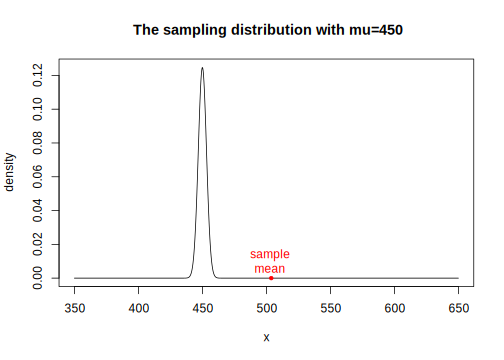
\includegraphics{Freq_CogSci_files/figure-latex/unnamed-chunk-43-1.pdf}

The intuitive idea here is that

\begin{itemize}
\tightlist
\item
  if the sample mean \(\bar{y}\) is ``near'' the hypothesized \(\mu\) (here, 450), the data are possibly (but by no means necessarily) consistent with the null hypothesis distribution.
\item
  if the sample mean \(\bar{y}\) is ``far'' from the hypothesized \(\mu\), the data are inconsistent with the null hypothesis distribution.
\end{itemize}

The terms ``near'' and ``far'' will be quantified by determining how many standard error units the sample mean is from the hypothesized mean. This way of thinking shifts the focus away from the sampling distribution above, towards the distance measured in standard error units from the null hypothesis mean.

The distance between the sample mean and the hypothesized mean can be written in SE units as follows. We will say that the sample mean is \(t\) standard errors away from the hypothesized mean:

\begin{equation}
t \times SE = \bar{x} - \mu 
\end{equation}

If we divide both sides with the standard error, we obtain the so-called observed t-statistic:

\begin{equation}
t  = \frac{\bar{x} - \mu}{SE}
\end{equation}

This observed t-value, an expression of the distance between the sample mean and the hypothesized mean, becomes the basis for the statistical test.

Notice that the t-value is a random variable: it is a transformation of \(\bar{X}\), the random variable generating the sample means. The t-value can therefore be seen as an instance of the following transformed random variable \(T\):

\begin{equation}
T  = \frac{\bar{X} - \mu}{SE}
\end{equation}

This random variable has a pdf associated with it, the t-distribution, which is defined in terms of the sample size \(n\); the pdf is written \(t(n-1)\). Under repeated sampling, the t-distribution is generated from this random variable \(T\).

We will compactly express the statement that ``the observed t-value is assumed to be generated (under repeated sampling) from a t-distribution with n-1 degrees of freedom'' as:

\begin{equation}
T \sim t(n-1)
\end{equation}

For large \(n\), the pdf of the random variable \(T\) approaches \(N(0,1)\). This is illustrated in Figure \ref{fig:tnormal}; notice that the t-distribution has fatter tails than the normal for small \(n\), say \(n<20\), but for larger n, the t-distribution and the normal become increasingly similar in shape. Incidentally, when n=2, the t-distribution \(t(1)\) is the Cauchy distribution we saw earlier; this distribution is characterized by fat tails, and has no mean or variance defined for it.

\begin{figure}
\centering
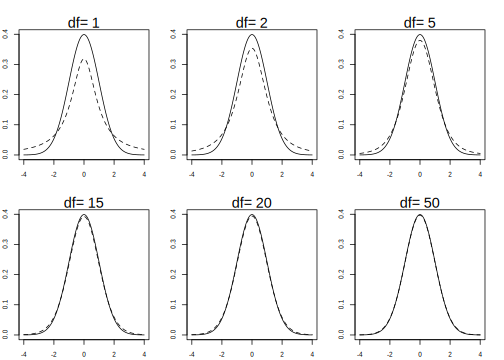
\includegraphics{Freq_CogSci_files/figure-latex/tnormal-1.pdf}
\caption{\label{fig:tnormal}A visual comparison of the t-distribution (with degrees of freedom ranging from 1 to 50) with the standard normal distribution (N(0,1)). The dashed line represents the t-distribution, and the solid line the normal distribution.}
\end{figure}

Thus, given a sample size \(n\), we can define a t-distribution corresponding to the null hypothesis distribution. For large values of \(n\), we could even use \(N(0,1)\), although it is traditional in psychology and linguistics to always use the t-distribution no matter how large \(n\) is.

The null hypothesis testing procedure proceeds as follows:

\begin{itemize}
\tightlist
\item
  Define the null hypothesis: in our example, the null hypothesis was that \(\mu = 450\). This amounts to making a commitment about what fixed value we think the true underlying distribution of sample means is centered at.
\item
  Given data of size \(n\), estimate \(\bar{y}\), standard deviation \(s\), and from that, estimate the standard error \(s/\sqrt{n}\). The standard error will be used to describe the sampling distribution's standard deviation.
\item
  Compute the observed t-value:
\end{itemize}

\begin{equation}
t=\frac{\bar{y}-\mu}{s/\sqrt{n}}
\end{equation}

\begin{itemize}
\tightlist
\item
  Reject null hypothesis if the observed t-value is ``large'' (to be made more precise next).
\item
  Fail to reject the null hypothesis, or (under some conditions, to be made clear later) even go so far as to accept the null hypothesis, if the observed t-value is ``small''.
\end{itemize}

What constitutes a large or small observed t-value?
Intuitively, the t-value from the sample is large when we end up far in \emph{either} tail of the distribution. The two tails of the t-distribution will be referred to as the \emph{rejection region}. The word \emph{region} here refers to the real number line along the x-axis, under the tails of the distribution. The rejection region will go off to infinity on the outer sides, and is demarcated by a vertical line on the inner side of each tail. This is shown in Figure \ref{fig:tails}. It goes off to infinity because the support---the range of possible values---of the random variable that the t-distribution belongs to stretches from minus infinity to plus infinity.

\begin{figure}
\centering
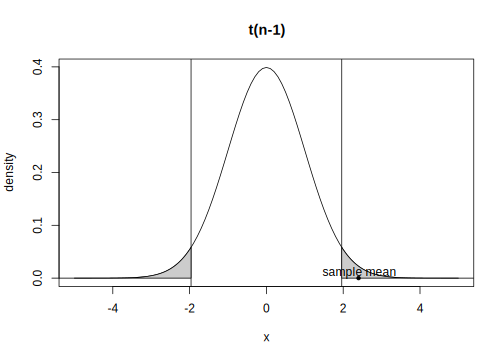
\includegraphics{Freq_CogSci_files/figure-latex/tails-1.pdf}
\caption{\label{fig:tails}The rejection region in a t-distribution. The rejection region is the x-axis under the gray-colored area.}
\end{figure}

The location of the vertical lines is determined by the so-called \emph{critical t-value} along the x-axis of the t-distribution. This is the value such that the area under the curve in the tails to the left or right of the tails is 0.025. As discussed in chapter 1, this area under the curve represents the probability of observing a value as extreme as the critical t-value, or some value that is more extreme. Notice that if we ask ourselves what the probability is of observing some particular t-value (a point value), the answer must necessarily be \(0\) (if you are unclear about why, re-read chapter 1). But we can ask the question: what is the absolute t-value, written \(|t|\), such that \(P(T>|t|)=0.025\)? That's the critical t-value. We call it the critical t-value because it demarcates the rejection region shown in Figure \ref{fig:tails}: we are adopting the convention that any observed t-value larger than this critical t-value allows us to reject the null hypothesis.

For a given sample size \(n\), we can identify the rejection region by using the \texttt{qt} function, whose usage is analogous to the \texttt{qnorm} function, discussed in chapter 1.

Because the shape of the t-distribution depends on the degrees of freedom (n-1), the critical t-value beyond which we reject the null hypothesis will change depending on sample size. For large sample sizes, say \(n>50\), the rejection point is about 2.

\begin{Shaded}
\begin{Highlighting}[]
\KeywordTok{abs}\NormalTok{(}\KeywordTok{qt}\NormalTok{(}\FloatTok{0.025}\NormalTok{,}\DataTypeTok{df=}\DecValTok{15}\NormalTok{))}
\end{Highlighting}
\end{Shaded}

\begin{verbatim}
## [1] 2.131
\end{verbatim}

\begin{Shaded}
\begin{Highlighting}[]
\KeywordTok{abs}\NormalTok{(}\KeywordTok{qt}\NormalTok{(}\FloatTok{0.025}\NormalTok{,}\DataTypeTok{df=}\DecValTok{50}\NormalTok{))}
\end{Highlighting}
\end{Shaded}

\begin{verbatim}
## [1] 2.009
\end{verbatim}

Consider the observed t-value from our sample in our running example:

\begin{Shaded}
\begin{Highlighting}[]
\CommentTok{## null hypothesis mean:}
\NormalTok{mu<-}\DecValTok{450}
\NormalTok{(t_value<-(y_bar}\OperatorTok{-}\NormalTok{mu)}\OperatorTok{/}\NormalTok{SE)}
\end{Highlighting}
\end{Shaded}

\begin{verbatim}
## [1] 16.82
\end{verbatim}

This observed t-value is huge and is telling you the distance of the sample mean from the null hypothesis mean \(\mu\) in standard error units.

\begin{equation}
t=\frac{\bar{y}-\mu_0}{s/\sqrt{n}} \hbox{ or } t\frac{s}{\sqrt{n}}=\bar{y}-\mu_0
\end{equation}

For large sample sizes, if the absolute t-value \(|t|\) is greater than \(2\), we will reject the null hypothesis.

For a smaller sample size \(n\), you can compute the exact critical t-value:

\begin{Shaded}
\begin{Highlighting}[]
\KeywordTok{qt}\NormalTok{(}\FloatTok{0.025}\NormalTok{,}\DataTypeTok{df=}\NormalTok{n}\DecValTok{-1}\NormalTok{)}
\end{Highlighting}
\end{Shaded}

\begin{verbatim}
## [1] -1.962
\end{verbatim}

Why is this critical t-value negative in sign? That is because it is on the left-hand side of the t-distribution, which is symmetric.
The corresponding value on the right-hand side is:

\begin{Shaded}
\begin{Highlighting}[]
\KeywordTok{qt}\NormalTok{(}\FloatTok{0.975}\NormalTok{,}\DataTypeTok{df=}\NormalTok{n}\DecValTok{-1}\NormalTok{)}
\end{Highlighting}
\end{Shaded}

\begin{verbatim}
## [1] 1.962
\end{verbatim}

These values are of course identical if we ignore the sign. This is why we always frame our discussion around the absolute t-value.

In R, the built-in function \texttt{t.test} delivers the observed t-value. Given our running example, with the null hypothesis \(\mu=450\), R returns the following:

\begin{Shaded}
\begin{Highlighting}[]
\CommentTok{## observed t-value from t-test function:}
\KeywordTok{t.test}\NormalTok{(y,}\DataTypeTok{mu=}\DecValTok{450}\NormalTok{)}\OperatorTok{$}\NormalTok{statistic}
\end{Highlighting}
\end{Shaded}

\begin{verbatim}
##     t 
## 16.82
\end{verbatim}

The default value for the null hypothesis mean \(\mu\) in this function is 0; so if one doesn't define a null hypothesis mean, the statistical test is done with reference to a null hypothesis that \(\mu=0\). That is why this t-value does not match our calculation above:

\begin{Shaded}
\begin{Highlighting}[]
\KeywordTok{t.test}\NormalTok{(y)}\OperatorTok{$}\NormalTok{statistic}
\end{Highlighting}
\end{Shaded}

\begin{verbatim}
##     t 
## 157.5
\end{verbatim}

In the most common usage of the t-test, the null hypothesis mean will be \(0\), because usually one is comparing a difference in means between two conditions or two sets of conditions. So the above line of code will work out correctly in those cases; but if you ever have a different null hypothesis mean than \(0\), then you have to specify it in the \texttt{t.test} function.

So, the way that the t-test is used in psychology and relate areas is to implement a \emph{decision}: either reject the null hypothesis or fail to reject it. Whenever we do an experiment and carry out a t-test, we use the t-test to make this binary decision: reject or fail to reject the null hypothesis.

Recall that behind the t-test lies the assumption that the observed t-value is coming from a random variable, \(T\sim t(n-1)\). The particular t-value we observe from a particular data-set belongs to a distribution of t-values under hypothetical repeated sampling. Thus, implicit in the logic of the t-test---and indeed every frequentist statistical test---is the assumption that the experiment is in principle repeatable: the experiment can in principle be re-run as many times as we want, assuming we have the necessary resources and time.

A quick simulation of t-values under repeated sampling makes this clear. Suppose that our null hypothesis mean is 450, and our sample size \(n=1000\). Assume that the data come from \(Normal(\mu=450,\sigma=100)\). Let's do 10000 simulations, compute the sample mean each time, and then store the observed t-value. The t-distribution that results is shown in Figure \ref{fig:simt}.

\begin{Shaded}
\begin{Highlighting}[]
\NormalTok{n<-}\DecValTok{1000}
\NormalTok{nsim<-}\DecValTok{10000}
\NormalTok{tvals<-}\KeywordTok{rep}\NormalTok{(}\OtherTok{NA}\NormalTok{,nsim)}
\ControlFlowTok{for}\NormalTok{(i }\ControlFlowTok{in} \DecValTok{1}\OperatorTok{:}\NormalTok{nsim)\{}
\NormalTok{y<-}\KeywordTok{rnorm}\NormalTok{(n,}\DataTypeTok{mean=}\DecValTok{450}\NormalTok{,}\DataTypeTok{sd=}\DecValTok{100}\NormalTok{)}
\NormalTok{SE<-}\KeywordTok{sd}\NormalTok{(y)}\OperatorTok{/}\KeywordTok{sqrt}\NormalTok{(n)}
\NormalTok{tvals[i]<-(}\KeywordTok{mean}\NormalTok{(y)}\OperatorTok{-}\DecValTok{450}\NormalTok{)}\OperatorTok{/}\NormalTok{SE}
\NormalTok{\}}
\KeywordTok{plot}\NormalTok{(}\KeywordTok{density}\NormalTok{(tvals),}\DataTypeTok{main=}\StringTok{"Simulated t-distribution"}\NormalTok{,}\DataTypeTok{xlab=}\StringTok{"t-values under repeated sampling"}\NormalTok{)}
\end{Highlighting}
\end{Shaded}

\begin{figure}
\centering
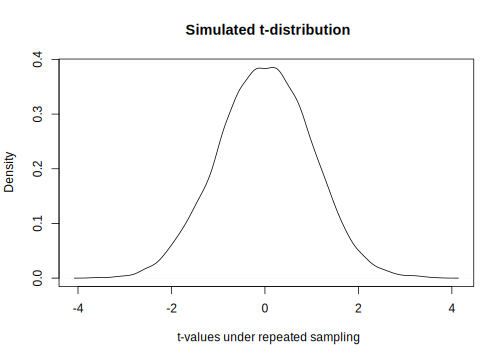
\includegraphics{Freq_CogSci_files/figure-latex/simt-1.pdf}
\caption{\label{fig:simt}The distribution of t-values under repeated sampling.}
\end{figure}

This implicit idea of the experiment's repeatability leads to an important aspect of the t-test: the proportion of times we would reject the null hypothesis under repeated sampling, given that the null is in fact true or false. In other words, we will now study the t-test's ability (at least in theory) to lead the researchers to the correct decision under (hypothetical) repeated sampling. We turn to this issue next.

\hypertarget{type-i-ii-error-and-power}{%
\subsection{Type I, II error, and power}\label{type-i-ii-error-and-power}}

When we do a hypothesis test using the t-test, the observed t-value will either fall in the rejection region, leading us to reject the null hypothesis,
or it will land in the non-rejection region, leading us to fail to reject the null. That is a single, one-time event.

So suppose we have made our decision based on the observed t-value. Now, the null hypothesis can be either true or not true; we don't know which of those two possibilities is the reality.
When we decide (based on the observed t-value) that the null is true, we are asserting that the parameter \(\mu\) actually does have the hypothesized value \(\mu_0\); when we decide that the null is false, we are asserting that the parameter \(\mu\) has some \emph{specific} value \(\mu_{alt}\) other than \(\mu_0\).
We can represent these two alternative possible realities in a tabular form, as shown in Table \ref{tab:type12}. The two columns show the two possible worlds, one in which the null is true, and the other in which it is false. The two rows show the two possible decisions we can take based on the observed t-value: reject the null or fail to reject it.

\begin{table}
\begin{tabular}{ccc}
        & \textbf{Possible world 1}      & \textbf{Possible world 2} \\  
\hline
 & $H_0$ TRUE: $\mu=\mu_0$  & $H_0$ FALSE $\mu=\mu_{alt}$ \\
\hline
Decision: `reject': & $\alpha$ & $1~-~\beta$ \\
                                     & Type I error                         & Power \\                                      
                                     & & \\
\hline
Decision: `fail to reject': & $1 - \alpha$ & $\beta$ \\                                    &                                 & Type II error\\
\hline
\end{tabular}
\caption{The possible realities (null is true or null is false) and the possible decisions (accept or reject null) we can take based on our observed t-value.} \label{tab:type12}
\end{table}

As the table shows, we can make two kinds of mistakes:

\begin{itemize}
\tightlist
\item
  Type I error or \(\alpha\): Reject the null when it's true.
\item
  Type II error or \(\beta\): Accept the null when it's false.
\end{itemize}

In psychology and related areas, Type I error is usually fixed a priori at 0.05. This stipulated Type I error value is why the absolute critical t-value is kept at approximately \(2\); if, following recommendations from \citet{benjamin2018redefine}, we were to stipulate that the Type I error be 0.005, then the critical t-value would have had to be set at:

\begin{Shaded}
\begin{Highlighting}[]
\KeywordTok{abs}\NormalTok{(}\KeywordTok{qt}\NormalTok{(}\FloatTok{0.0025}\NormalTok{,}\DataTypeTok{df=}\NormalTok{n}\DecValTok{-1}\NormalTok{))}
\end{Highlighting}
\end{Shaded}

\begin{verbatim}
## [1] 2.813
\end{verbatim}

This suggested change in convention hasn't been taken up yet in cognitive science, but this could well change one day.

Type II error, the probability of incorrectly accepting the null hypothesis when it is false with some particular value for the parameter \(\mu\), is conventionally recommended \citep{powerbookcohen} to be kept at 0.20 or lower. This implies that the probability of correctly rejecting a null hypothesis for some particular true value of \(\mu\) is 1-Type II error. This probability, called statistical power, or just power, should then obviously be larger than 0.80. Again, there is nothing special about these stipulations; they are conventions that became the norm over time.

Next, we will consider the trade-off between Type I and II error. For simplicity, assume that the standard error is 1, and the null hypothesis is that \(\mu=0\). This means that the observed t-value is really the sample mean.

Consider the concrete situation where, in reality, the true value of \(\mu\) is \(2\). As mentioned above, the null hypothesis \(H_0\) is that \(\mu=0\). Now the \(H_0\) is false because \(\mu=2\) and not \(0\). Type I and II error can be visualized graphically as shown in Figure \ref{fig:type12}.

\begin{figure}
\centering
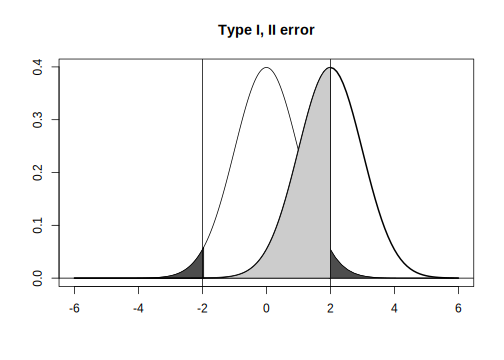
\includegraphics{Freq_CogSci_files/figure-latex/type12-1.pdf}
\caption{\label{fig:type12}A visualization of Type I and II error. The dark-shaded tails of the left-hand side distribution represent Type I error; and the light-colored shaded region of the right-hand side distribution represents Type II error. Power is the unshaded area under the curve in the right-hand side distribution.}
\end{figure}

To understand Figure \ref{fig:type12}, one has to consider two distributions side by side. First, consider the null hypothesis distribution, centered at 0. Under the null hypothesis distribution, the rejection region lies below the dark colored tails of the distributions. The area under the curve in these dark-colored tails is the Type I error (conventionally set at 0.05) that we decide on before we even conduct the experiment and collect the data. Because the Type I error is set at 0.05, and because the t-distribution is symmetric, the area under the curve in each tail is 0.025. The absolute critical t-value helps us demarcate the inner boundaries of the rejection regions through the vertical lines shown in the figure. These vertical lines play a crucial role in helping us understand Type II error and power. This becomes clear when we consider the distribution representing the alternative possible value of \(\mu\), the distribution centered around 2. In this second distribution, consider now the area under the curve between the vertical lines demarcating the rejection region under the null. This area under the curve is the probability of accepting the null hypothesis when the null hypothesis is false with some specific value (here, when \(\mu\) has value 2).

Some interesting observations follow. Suppose that the true effect is in fact \(\mu=2\), as in the above illustration. Then,

\begin{itemize}
\tightlist
\item
  Simply decreasing Type I error to a smaller value like 0.005 will increase Type II error, which means that power (1-Type II error) will fall.
\item
  Increasing sample size will squeeze the vertical lines closer to each other because standard error will go down with increasing sample size. This will reduce Type II error, and therefore increase power. Decreasing sample size will have the opposite effect.
\item
  If we design an experiment with a larger effect size, e.g., by setting up a stronger manipulation (concete examples will be discussed in this book later on), our Type II error will go down, and therefore power will go up. Figure \ref{fig:highpower} shows a graphical visualization of a situation where the true effect size is \(\mu=4\). Here, Type II error is much smaller compared to Figure \ref{fig:type12}, where \(\mu=2\).
\end{itemize}

\begin{figure}
\centering
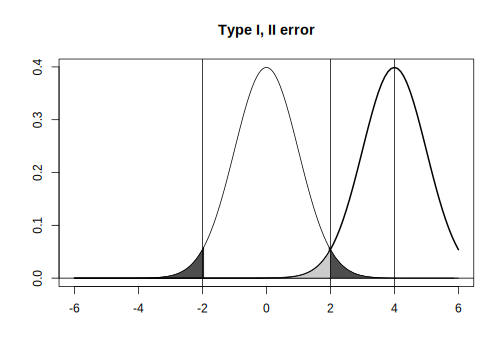
\includegraphics{Freq_CogSci_files/figure-latex/highpower-1.pdf}
\caption{\label{fig:highpower}The change in Type II error if the true effect has mean 4.}
\end{figure}

In summary, when we plan out an experiment, we are also required to specify the Type I and II error associated with the design. Both sources of error are within our control, at least to some extent. The Type I error we decide to use will determine our critical t-value and therefore our decision criterion for rejecting, failing to reject, or even (under certain conditions, to be discussed below) accepting the null hypothesis.

The Type II error we decide on will determine the long-run probability of incorrectly accepting the null hypothesis; its inverse (1-Type II error), statistical power, will determine the long-run probability of correctly rejecting the null hypothesis under the assumption that the \(\mu\) has some particular assumed value.

That's the theory anyway. In practice, researchers only rarely consider the power properties of their experiment design; the focus is almost exclusively on Type I error. The neglect of power in experiment design has had interesting consequences for theory development, as we will see later in this book. For a case study in psycholinguistics, see \citet{VasishthMertzenJaegerGelman2018}.

\hypertarget{how-to-compute-power-for-the-one-sample-t-test}{%
\subsection{How to compute power for the one-sample t-test}\label{how-to-compute-power-for-the-one-sample-t-test}}

Power (which is 1-Type II error) is a function of three variables:

\begin{itemize}
\tightlist
\item
  the effect size
\item
  the standard deviation
\item
  the sample size.
\end{itemize}

There are two ways that one can compute power in connection with the t-test: either one can use the built-in R function, \texttt{power.t.test}, or one can use simulation.

\hypertarget{power-calculation-using-the-power.t.test}{%
\subsubsection{Power calculation using the power.t.test}\label{power-calculation-using-the-power.t.test}}

Suppose that we have an expectation that an effect size is 15 ms \(\pm 5\) ms (this could be based on the predictions of a theoretical model, or prior data); suppose also that prior experiments show standard deviations ranging from 100 to 300 ms. This is enough information to compute a power curve as a function of effect size and standard deviation. See Figure \ref{fig:powercurve} and the associated code below.

\begin{Shaded}
\begin{Highlighting}[]
\NormalTok{sds<-}\KeywordTok{seq}\NormalTok{(}\DecValTok{100}\NormalTok{,}\DecValTok{300}\NormalTok{,}\DataTypeTok{by=}\DecValTok{1}\NormalTok{)}
\NormalTok{lower<-}\KeywordTok{power.t.test}\NormalTok{(}\DataTypeTok{delta=}\DecValTok{15-5}\NormalTok{,}\DataTypeTok{sd=}\NormalTok{sds,}\DataTypeTok{n=}\DecValTok{10}\NormalTok{,}\DataTypeTok{strict =}\OtherTok{TRUE}\NormalTok{)}\OperatorTok{$}\NormalTok{power}
\NormalTok{upper<-}\KeywordTok{power.t.test}\NormalTok{(}\DataTypeTok{delta=}\DecValTok{15}\OperatorTok{+}\DecValTok{5}\NormalTok{,}\DataTypeTok{sd=}\NormalTok{sds,}\DataTypeTok{n=}\DecValTok{10}\NormalTok{,}\DataTypeTok{strict =}\OtherTok{TRUE}\NormalTok{)}\OperatorTok{$}\NormalTok{power}
\NormalTok{meanval<-}\KeywordTok{power.t.test}\NormalTok{(}\DataTypeTok{delta=}\DecValTok{15}\NormalTok{,}\DataTypeTok{sd=}\NormalTok{sds,}\DataTypeTok{n=}\DecValTok{10}\NormalTok{,}\DataTypeTok{strict =}\OtherTok{TRUE}\NormalTok{)}\OperatorTok{$}\NormalTok{power}

\KeywordTok{plot}\NormalTok{(sds,meanval,}\DataTypeTok{type=}\StringTok{"l"}\NormalTok{,}
     \DataTypeTok{main=}\StringTok{"Power curve (n=10)}\CharTok{\textbackslash{}n}\StringTok{ }
\StringTok{     using power.t.test"}\NormalTok{,}
     \DataTypeTok{xlab=}\StringTok{"standard deviation"}\NormalTok{,}
     \DataTypeTok{ylab=}\StringTok{"power"}\NormalTok{)}
\KeywordTok{lines}\NormalTok{(sds,lower,}\DataTypeTok{lty=}\DecValTok{2}\NormalTok{)}
\KeywordTok{lines}\NormalTok{(sds,upper,}\DataTypeTok{lty=}\DecValTok{2}\NormalTok{)}
\KeywordTok{text}\NormalTok{(}\DecValTok{125}\NormalTok{,}\FloatTok{0.053}\NormalTok{,}\StringTok{"10"}\NormalTok{)}
\KeywordTok{text}\NormalTok{(}\DecValTok{150}\NormalTok{,}\FloatTok{0.054}\NormalTok{,}\StringTok{"15"}\NormalTok{)}
\KeywordTok{text}\NormalTok{(}\DecValTok{175}\NormalTok{,}\FloatTok{0.056}\NormalTok{,}\StringTok{"20"}\NormalTok{)}
\end{Highlighting}
\end{Shaded}

\begin{figure}
\centering
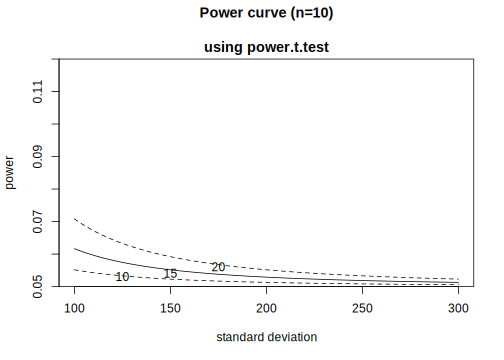
\includegraphics{Freq_CogSci_files/figure-latex/powercurve-1.pdf}
\caption{\label{fig:powercurve}An illustration of a power curve for 10 participants, as a function of standard deviation, and three estimates of the effect: 15, 10, and 20.}
\end{figure}

\hypertarget{power-calculations-using-simulation}{%
\subsubsection{Power calculations using simulation}\label{power-calculations-using-simulation}}

An analogous calculation as the one shown above using the \texttt{power.t.test} function can also be done using simulated data.
First, generate simulated data repeatedly for each possible combination of parameter values (here, effect size and standard deviation), and compute the proportion of significant effects for each parameter combination. This can be done by defining a function that takes as input the number of simulations, sample size, effect size, and standard deviation:

\begin{Shaded}
\begin{Highlighting}[]
\NormalTok{compute_power<-}\ControlFlowTok{function}\NormalTok{(}\DataTypeTok{nsim=}\DecValTok{1000}\NormalTok{,}\DataTypeTok{n=}\DecValTok{10}\NormalTok{,}
                        \DataTypeTok{effect =} \OtherTok{NULL}\NormalTok{,}
                        \DataTypeTok{stddev=}\OtherTok{NULL}
\NormalTok{                        )\{}
\NormalTok{  temp_power<-}\KeywordTok{rep}\NormalTok{(}\OtherTok{NA}\NormalTok{,nsim)}
  \ControlFlowTok{for}\NormalTok{(i }\ControlFlowTok{in} \DecValTok{1}\OperatorTok{:}\NormalTok{nsim)\{}
\NormalTok{   y<-}\KeywordTok{rnorm}\NormalTok{(n,}\DataTypeTok{mean=}\NormalTok{effect,}\DataTypeTok{sd=}\NormalTok{stddev)}
\NormalTok{   temp_power[i]<-}\KeywordTok{ifelse}\NormalTok{(}\KeywordTok{abs}\NormalTok{(}\KeywordTok{t.test}\NormalTok{(y)}\OperatorTok{$}\NormalTok{statistic)}\OperatorTok{>}\DecValTok{2}\NormalTok{,}\DecValTok{1}\NormalTok{,}\DecValTok{0}\NormalTok{)}
\NormalTok{  \}}
  \CommentTok{## return power calculation:}
  \KeywordTok{mean}\NormalTok{(temp_power)}
\NormalTok{\}}
\end{Highlighting}
\end{Shaded}

Then, plot the power curves as a function of effect size and standard deviation, exactly as in Figure \ref{fig:powercurve}. Power calculations using simulations are shown in Figure \ref{fig:powercurve2}. It is clear that simulation-based power estimation is going to be noisy; this is because each time we are generating simulated data and then carrying out a statistical test on it. This is no longer a closed-form mathematical calculation as done in \texttt{power.t.test} (this function simply implements a formula for power calculation specified for this simple case). Because the power estimates will be noisy, we show a smoothed lowess line for each effect size estimate.

\begin{figure}
\centering
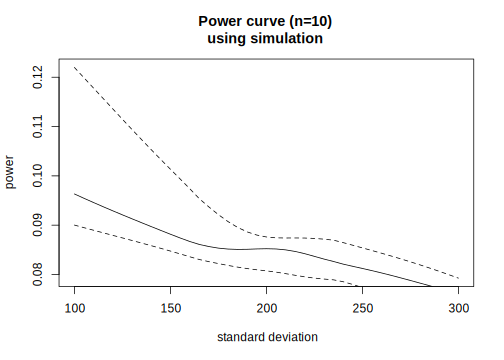
\includegraphics{Freq_CogSci_files/figure-latex/powercurve2-1.pdf}
\caption{\label{fig:powercurve2}An illustration of a power curve using simulation, for 10 participants, as a function of standard deviation, and three estimates of the effect: 15, 10, and 20. The power curves are lowess-smoothed.}
\end{figure}

In the above example, simulation-based power calculation is overkill, and completely unnecessary because we have \texttt{power.t.test}. However, the technique shown above will be extended and will become our bread-and-butter method once we switch to power calculations for complicated linear mixed models. There, no closed form calculation can be done to compute power, at least not without oversimplifying the model; simulation will be the only practical way to calculate power.

It is important to appreciate the fact that power is a \emph{function}; it isn't a single number. Because we can never be sure what the true effect size is, or what the true standard deviation is, power functions (power as a function of plausible values for the relevant parameters) are much more useful than single numbers.

\hypertarget{the-p-value}{%
\subsection{The p-value}\label{the-p-value}}

Continuing with our t-test example, the \texttt{t.test} function in R will not only print out a t-value as shown above, but also a probability known as a \emph{p-value}. This is the probability of obtaining the observed t-value that we obtained, or some value more extreme than that, conditional on the assumption that the null hypothesis is true.

We can compute the p-value ``by hand''. This can be computed, as done earlier, simply by calculating the area under the curve that lies beyond the observed t-value. It is standard practice to take the tail probability on both sides of the t-distribution.

\begin{Shaded}
\begin{Highlighting}[]
\NormalTok{(t_value<-}\KeywordTok{t.test}\NormalTok{(y,}\DataTypeTok{mu=}\DecValTok{450}\NormalTok{)}\OperatorTok{$}\NormalTok{statistic)}
\end{Highlighting}
\end{Shaded}

\begin{verbatim}
##         t 
## -0.008827
\end{verbatim}

\begin{Shaded}
\begin{Highlighting}[]
\DecValTok{2}\OperatorTok{*}\KeywordTok{pt}\NormalTok{(}\KeywordTok{abs}\NormalTok{(t_value),}\DataTypeTok{df=}\NormalTok{n}\DecValTok{-1}\NormalTok{,}\DataTypeTok{lower.tail=}\OtherTok{FALSE}\NormalTok{)}
\end{Highlighting}
\end{Shaded}

\begin{verbatim}
##      t 
## 0.9931
\end{verbatim}

The area from both sides of the tail is taken because it is conventional to do a so-called \emph{two-sided t-test}: our null hypothesis is that \(\mu=450\), and our alternative hypothesis is two-sided: \(\mu\) is either less than 450 or \(\mu\) is larger than 450. When we reject the null hypothesis, we are accepting this alternative, that \(\mu\) could be some value other than 450. Notice that this alternative hypothesis is remarkably vague; we would reject the null hypothesis regardless of whether the sample mean turns out to be 600 or -600, for example. The practical implication is that the p-value gives us the strength of the evidence against the null hypothesis; it doesn't give us evidence in favor of a specific alternative, such as saying that \(\mu\) is positive or negative in sign. In psychology and allied disciplines, whenever the p-value falls below \(0.05\), it is common practice to write something along the lines that ``there was reliable evidence for the predicted effect.'' This statement is incorrect! We only ever have evidence against the null. By looking at the sample mean and its sign, we are making a very big leap that we have evidence for the specific sample mean we happened to get. As we will see below, the sample mean can be wildly far from the true mean that produced the data.

One need not have a two-sided alternative; one could have defined the alternative to be one-sided (for example, that \(mu>450\)). In that case, one would compute only one side of the area under the curve. This kind of one-sided test is not normally done, but one can imagine a situation where a one-sided test is justified (for example, when only one sign of the effect is possible, or if there is a strong theoretical reason to expect only one particular sign---positive or negative---on an effect). That said, in their scientific career, only one of the authors of this book has ever had occasion to use a one-sided test. In this book, we will not use one-sided t-tests.

The p-value is always interpreted with reference to the pre-defined Type I error. Conventionally, we reject the null if \(p<0.05\). This is because we set the Type I error at 0.05. Keep in mind that Type I error and the p-value are two distinct things.
Type I error is the probability of your incorrectly rejecting the null under repeated sampling. This is not the same thing as your p-value. The latter will be obtained from a particular experiment, and will vary from experiment to experiment; it is a random variable. Type I error is a value we fix in advance.

\hypertarget{the-distribution-of-the-p-value-under-the-null-hypothesis}{%
\subsubsection{*The distribution of the p-value under the null hypothesis}\label{the-distribution-of-the-p-value-under-the-null-hypothesis}}

We have been talking about a continuous random variable as a dependent measure, and have learnt about the standard two-sided t-test, with a point null hypothesis. When we do such a test, we usually use the p-value to decide whether to reject the null hypothesis or not.

Sometimes, you will hear statisticians (e.g., Andrew Gelman on his blog) criticize p-values by saying that the null hypothesis significance test is a ``specific random number generator''. What does that sentence mean? We explain this point here because it is important for understanding the meaning of the p-value.

Suppose that the null hypothesis is in fact true. We will now simulate the distribution of the p-value under repeated sampling:

\begin{figure}
\centering
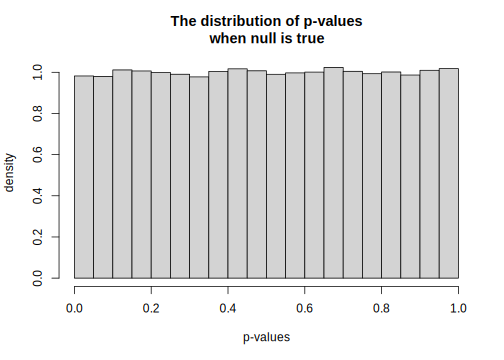
\includegraphics{Freq_CogSci_files/figure-latex/pvalnulltrue-1.pdf}
\caption{\label{fig:pvalnulltrue}The p-value has a uniform distribution when the null hypothesis is true; a demonstration using simulation.}
\end{figure}

The distribution of the p-value is uniform---every value between 0 and 1 is equally likely.

We will now formally derive the above fact, that the distribution of the p-value is uniform under the null hypothesis.

Consider the fact that the p-value is a random variable; call it \(Z\). The p-value is the cumulative distribution function (CDF) of the random variable \(T\), which itself is a transformation of the random variable \(\bar{Y}\):

\(T=(\bar{X}-\mu)/(\sigma/\sqrt{n})\)

This random variable \(T\) has some CDF \(F(T)\). It is possible to show that if a random variable \(Z=F(T)\), i.e., if \(Z\) is the
CDF for the random variable \(T\), then \(Z\) has a uniform distribution ranging from 0 to 1, \(Z \sim Uniform(0,1)\).

This is an amazing fact. To get a grip on this, let's first think about the fact that when a random variable \(Z\) comes from a \(Uniform(0,1)\) distribution, then \(P(Z<z)=z\). Consider some examples:

\begin{itemize}
\tightlist
\item
  when \(z=0\), then \(P(Z<0)=0\);
\item
  when \(z=0.25\), then \(P(Z<0.25)=0.25\);
\item
  when \(z=0.5\), then \(P(Z<0.5)=0.5\);
\item
  when \(z=0.75\), then \(P(Z<0.75)=0.75\);
\item
  when \(z=1\), then \(P(Z<1)=1\).
\end{itemize}

Next, we will prove the above statement, that if a random variable \(Z=F(T)\), i.e., if \(Z\) is the
CDF for a random variable \(T\), then \(Z \sim Uniform(0,1)\).
The proof is actually quite astonishing and even has a name: it's called the \emph{probability integral transform}.

Suppose that \(Z\) is the CDF of a random variable \(T\): \(Z=F(T)\). Then, it follows that \(P(Z\leq z)\) can be rewritten in terms of the CDF of T: \(P(F(T)\leq z)\). Now, if we apply the inverse of the CDF (\(F^{-1}\)) to both the left and right sides of the inequality, we get \(P(F^{-1}F(T)\leq F^{-1}(z))\).
But \(F^{-1}F(T)\) gives us back \(T\); this holds because if we have a one-to-one onto function \(f(x)\), then applying the inverse \(f^{-1}\) to this function gives us back \(x\).

The fact that \(F^{-1}F(T)\) gives us back \(T\) means that we can rewrite \(P(F^{-1}F(T)\leq F^{-1}(z))\) as \(P(T\leq F^{-1}(z) )\). But this probability is simply the CDF \(F(F^{-1} (z))\), which simplifies to \(z\). This shows that \(P(Z\leq z) = z\); i.e., that the p-value has a uniform distribution under the null hypothesis.

The above proof is restated below compactly:

\begin{equation}
\begin{split}
P(Z\leq z) =& P(F(T)\leq z)\\
=& P(F^{-1}F(T)\leq F^{-1}(z))\\
=& P(T\leq F^{-1}(z) ) \\
=& F(F^{-1} (z))\\
=& z\\
\end{split}
\end{equation}

It is for this reason that statisticians like Andrew Gelman periodically point out that ``the null hypothesis significance test is a specific random number generator''. The practical implication of this criticism of p-values is that when we do a single experiment and obtain a p-value under the assumption that the null is true, if the null were in fact true, then we are just using a random number generator to make a decision that the effect is present or absent. A broader implication is that we should not place our theory development exclusively at the feet of the p-value. As we discuss in this book, other considerations (such as replicability, uncertainty of the estimates, and power) are as or even more important.

\hypertarget{type-m-and-s-error-in-the-face-of-low-power}{%
\subsection{Type M and S error in the face of low power}\label{type-m-and-s-error-in-the-face-of-low-power}}

Beyond Type I and II error, there are also two other kinds of error to be aware of. These are Type M and S error; both sources of error are closely related to statistical power.

The terms Type M and S error were introduced by \citet{Gelman14}, but the ideas have been in existence for some time \citep{hedges1984estimation},\citep{lane1978estimating}. \citet{powerfailure} refer to Type M and S error as the ``winner's curse'' and ``the vibration of effects.'' In related work, \citet{ioannidis2008most} refers to the vibration ratio in the context of epidemiology.

Type S and M error can be illustrated with the following example.
Suppose your true effect size is believed to be \(D=15\),
then we can compute (apart from statistical power) the following error rates, which are defined as follows:

\begin{itemize}
\tightlist
\item
  \textbf{Type S error}: the probability that the sign of the effect is incorrect, given that the result is statistically significant.
\item
  \textbf{Type M error}: the expectation of the ratio of the absolute magnitude of the effect to the hypothesized true effect size, given that the result is significant.
  Gelman and Carlin also call this the exaggeration ratio, which is perhaps more descriptive than ``Type M error''.
\end{itemize}

Suppose that a particular study has standard error \(46\), and sample size \(37\). And suppose that the true \(\mu=15\), as in the example discussed above. Then, we can compute statistical power, Type S and M error through simulation in the following manner:

\begin{Shaded}
\begin{Highlighting}[]
\CommentTok{## probable effect size, derived from past studies:}
\NormalTok{D<-}\DecValTok{15}
\CommentTok{## SE from the study of interest:}
\NormalTok{se<-}\DecValTok{46}
\NormalTok{stddev<-se}\OperatorTok{*}\KeywordTok{sqrt}\NormalTok{(}\DecValTok{37}\NormalTok{)}
\NormalTok{nsim<-}\DecValTok{10000}
\NormalTok{drep<-}\KeywordTok{rep}\NormalTok{(}\OtherTok{NA}\NormalTok{,nsim)}
\ControlFlowTok{for}\NormalTok{(i }\ControlFlowTok{in} \DecValTok{1}\OperatorTok{:}\NormalTok{nsim)\{}
\NormalTok{samp<-}\KeywordTok{rnorm}\NormalTok{(}\DecValTok{37}\NormalTok{,}\DataTypeTok{mean=}\NormalTok{D,}\DataTypeTok{sd=}\NormalTok{stddev)}
\NormalTok{drep[i]<-}\KeywordTok{mean}\NormalTok{(samp)}
\NormalTok{\}}
\end{Highlighting}
\end{Shaded}

Power can be computed by simply determining the proportion of times that the absolute observed t-value is larger than 2:

\begin{Shaded}
\begin{Highlighting}[]
\CommentTok{##power: the proportion of cases where }
\CommentTok{## we reject the null hypothesis correctly:}
\NormalTok{(pow<-}\KeywordTok{mean}\NormalTok{(}\KeywordTok{ifelse}\NormalTok{(}\KeywordTok{abs}\NormalTok{(drep}\OperatorTok{/}\NormalTok{se)}\OperatorTok{>}\DecValTok{2}\NormalTok{,}\DecValTok{1}\NormalTok{,}\DecValTok{0}\NormalTok{)))}
\end{Highlighting}
\end{Shaded}

\begin{verbatim}
## [1] 0.0589
\end{verbatim}

Power is quite low here (we deliberately chose an example with low power to illustrate Type S and M error).

Next, we figure out which of the samples are statistically significant (which simulated values yield \(p<0.05\)). As a criterion, we use a t-value of 2 to declare that we reject the null; we could have done this more precisely by working out an exact critical t-value.

\begin{Shaded}
\begin{Highlighting}[]
\CommentTok{## which results in drep are significant at alpha=0.05?}
\NormalTok{signif<-}\KeywordTok{which}\NormalTok{(}\KeywordTok{abs}\NormalTok{(drep}\OperatorTok{/}\NormalTok{se)}\OperatorTok{>}\DecValTok{2}\NormalTok{)}
\end{Highlighting}
\end{Shaded}

Type S error is the proportion of significant cases with the wrong sign (sign error), and Type M error is the ratio by which the true effect (of \(\mu=15\)) is exaggerated in those simulations that happened to come out significant.

\begin{Shaded}
\begin{Highlighting}[]
\CommentTok{## Type S error rate | signif:}
\NormalTok{(types_sig<-}\KeywordTok{mean}\NormalTok{(drep[signif]}\OperatorTok{<}\DecValTok{0}\NormalTok{))}
\end{Highlighting}
\end{Shaded}

\begin{verbatim}
## [1] 0.1902
\end{verbatim}

\begin{Shaded}
\begin{Highlighting}[]
\CommentTok{## Type M error rate | signif: }
\NormalTok{(typem_sig<-}\KeywordTok{mean}\NormalTok{(}\KeywordTok{abs}\NormalTok{(drep[signif])}\OperatorTok{/}\NormalTok{D))}
\end{Highlighting}
\end{Shaded}

\begin{verbatim}
## [1] 7.408
\end{verbatim}

In this scenario, when power is approximately 6\%, whenever we get a significant effect, the probability of obtaining the wrong sign is a whopping 19\% and the effect is likely to be 7.4078 times larger than its true magnitude. The practical implication is as follows.

When power is low, relying on the p-value (statistical significance) to declare an effect as being present will be misleading because the decision will be based on an overestimate of the effect (Type M error), and even the sign of the effect could be wrong. This isn't just a theoretical point; it has real-world consequences for theory development. For an example from psycholinguistics regarding this point, see \citet{VasishthMertzenJaegerGelman2018}.

Another useful way to visualize Type M and S error is through the so-called funnel plot. As shown in Figure \ref{fig:funnel}, estimates obtained from low-powered studies will tend to be exaggerated (the lower part of the funnel), and as power goes up, the effect estimates start to cluster tightly around the true value of the effect.

\begin{figure}
\centering
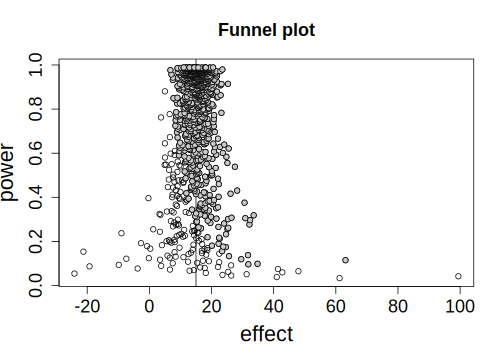
\includegraphics{Freq_CogSci_files/figure-latex/funnel-1.pdf}
\caption{\label{fig:funnel}An illustration of a funnel plot. Shown are repeated samples of an effect estimate under different values of power, where the true value of the effect is 15 (marked by the vertical line). Significant effects are shaded gray. The lower the power, the wider the fluctuation of the effect; under low power, it is the exaggerated effects that end up statistically significant, even though they are very biased relative to the true value. As power goes up, the effect estimates start to cluster around the true value, and significant effects are also accurate estimates of the effect. Thus, low power leads to exaggerated estimates of the effect, especially if the data are filtered by statistical significance.}
\end{figure}

What is important to appreciate here is the fact that significant effects ``point to the truth'' just in case power is high; when power is low, either null results will frequently be found even if the null is false, and those results that turn out significant will be based on Type M error.

In many fields, it is practically impossible to conduct a high-powered study. What should one do in this situation? When reporting results that are likely based on an underpowered study, the best approach is to openly acknowledge the power limitation, to attempt to conduct a direct replication of the effect to establish robustness, and to attempt to synthesize the evidence from existing knowlege \citep{cumming2014new}.

By direct replication, we mean that the study should be run multiple times with the same materials and design but new participants, to establish whether effect estimates in the original study and the replication study are consistent with each other. Direct replications stand in contrast to so-called conceptual replications, which are not exact repetitions of the original design, but involve some further or slightly different but related experimental manipulations. Conceptual replications are also a very useful tool for cross-validating the existence of an effect.

Direct replications will always differ from the original study in some way or another---the lab may differ, the protocols might differ slightly, the experimenter is different, etc. Such between-study variability is obviously unavoidable in direct-replication attempts, but they are still worthwhile for establishing the existence of an effect. To make more clear the idea of establishing robustness through replication attempts, detailed examples of different kinds of replication attempts of published studies will be presented in this book's example data-sets.

\hypertarget{searching-for-significance}{%
\subsection{Searching for significance}\label{searching-for-significance}}

The NHST procedure is essentially a decision procedure: if \(p<0.05\), we reject the null hypothesis; otherwise, we fail to reject the null. Because significant results are easier to publish than non-significant results, a common approach taken by researchers (including the first author of this book, when he was a graduate student) is to run the experiment and periodically check if statistical significance has been reached. The procedure can be described as follows:

\begin{itemize}
\tightlist
\item
  The experimenter gathers \(n\) data points, then checks for significance (is \(p<0.05\) or not?).
\item
  If the result is not significant, he gets more data (say, \(n\) more data points). Then he checks for significance, and repeats.
\end{itemize}

Since time and money are limited, he might decide to stop collecting data after some multiple of \(n\) have been collected.

One can simulate different scenarios here. Suppose that \(n\) is initially \(15\).\\
Under the standard assumptions, we set Type I error to be \(0.05\). Let's suppose that the null hypothesis that \(\mu=0\) is in fact true, and that standard deviation is 250.

\begin{Shaded}
\begin{Highlighting}[]
\CommentTok{##Standard properties of the t-test:}
\NormalTok{pvals<-}\OtherTok{NULL}
\NormalTok{tstat_standard<-}\OtherTok{NULL}
\NormalTok{n<-}\DecValTok{15}
\NormalTok{nsim<-}\DecValTok{10000}
\CommentTok{## assume a standard dev of 1:}
\NormalTok{stddev<-}\DecValTok{250}
\NormalTok{mn<-}\DecValTok{0}
\ControlFlowTok{for}\NormalTok{(i }\ControlFlowTok{in} \DecValTok{1}\OperatorTok{:}\NormalTok{nsim)\{}
\NormalTok{  samp<-}\KeywordTok{rnorm}\NormalTok{(n,}\DataTypeTok{mean=}\NormalTok{mn,}\DataTypeTok{sd=}\NormalTok{stddev)}
\NormalTok{  pvals[i]<-}\KeywordTok{t.test}\NormalTok{(samp)}\OperatorTok{$}\NormalTok{p.value}
\NormalTok{  tstat_standard[i]<-}\KeywordTok{t.test}\NormalTok{(samp)}\OperatorTok{$}\NormalTok{statistic}
\NormalTok{\}}
\end{Highlighting}
\end{Shaded}

Type I error rate is about 5\%, consistent with our expectations:

\begin{Shaded}
\begin{Highlighting}[]
\KeywordTok{round}\NormalTok{(}\KeywordTok{mean}\NormalTok{(pvals}\OperatorTok{<}\FloatTok{0.05}\NormalTok{),}\DecValTok{2}\NormalTok{)}
\end{Highlighting}
\end{Shaded}

\begin{verbatim}
## [1] 0.05
\end{verbatim}

But the situation quickly deteriorates as soon as we adopt the strategy outlined above. Below, we will also track the distribution of the t-statistic.

\begin{Shaded}
\begin{Highlighting}[]
\NormalTok{pvals<-}\OtherTok{NULL}
\NormalTok{tstat<-}\OtherTok{NULL}
\CommentTok{## how many subjects can I run?}
\NormalTok{upper_bound<-n}\OperatorTok{*}\DecValTok{6}

\ControlFlowTok{for}\NormalTok{(i }\ControlFlowTok{in} \DecValTok{1}\OperatorTok{:}\NormalTok{nsim)\{}
\NormalTok{  significant<-}\OtherTok{FALSE} 
\NormalTok{  x<-}\KeywordTok{rnorm}\NormalTok{(n,}\DataTypeTok{mean=}\NormalTok{mn,}\DataTypeTok{sd=}\NormalTok{stddev) }\CommentTok{## take sample}
\ControlFlowTok{while}\NormalTok{(}\OperatorTok{!}\NormalTok{significant }\OperatorTok{&}\StringTok{ }\KeywordTok{length}\NormalTok{(x)}\OperatorTok{<}\NormalTok{upper_bound)\{}
  \CommentTok{## if not significant:}
\ControlFlowTok{if}\NormalTok{(}\KeywordTok{t.test}\NormalTok{(x)}\OperatorTok{$}\NormalTok{p.value}\OperatorTok{>}\FloatTok{0.05}\NormalTok{)\{}
\NormalTok{  x<-}\KeywordTok{append}\NormalTok{(x,}\KeywordTok{rnorm}\NormalTok{(n,}\DataTypeTok{mean=}\NormalTok{mn,}\DataTypeTok{sd=}\NormalTok{stddev)) }\CommentTok{## get more data}
\NormalTok{\} }\ControlFlowTok{else}\NormalTok{ \{significant<-}\OtherTok{TRUE}\NormalTok{\}   }\CommentTok{## otherwise stop:}
\NormalTok{\}}
\NormalTok{pvals[i]<-}\KeywordTok{t.test}\NormalTok{(x)}\OperatorTok{$}\NormalTok{p.value}
\NormalTok{tstat[i]<-}\KeywordTok{t.test}\NormalTok{(x)}\OperatorTok{$}\NormalTok{statistic}
\NormalTok{\}}
\end{Highlighting}
\end{Shaded}

Now, Type I error rate is much higher than 5\%:

\begin{Shaded}
\begin{Highlighting}[]
\KeywordTok{round}\NormalTok{(}\KeywordTok{mean}\NormalTok{(pvals}\OperatorTok{<}\FloatTok{0.05}\NormalTok{),}\DecValTok{2}\NormalTok{)}
\end{Highlighting}
\end{Shaded}

\begin{verbatim}
## [1] 0.15
\end{verbatim}

Figure \ref{fig:stoppingrule} shows the distributions of the t-statistic in the standard case vs with the above stopping rule:

\begin{figure}
\centering
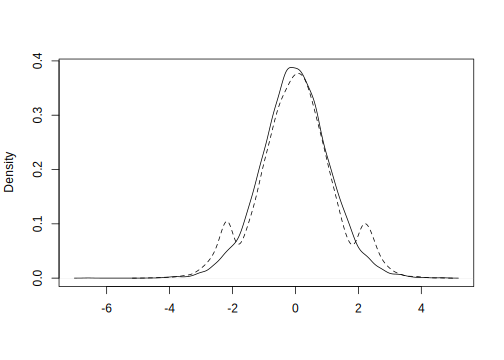
\includegraphics{Freq_CogSci_files/figure-latex/stoppingrule-1.pdf}
\caption{\label{fig:stoppingrule}A comparison of the distribution of t-values with an a priori fixed stopping rule, versus a flexible stopping rule conditional on finding significance.}
\end{figure}

What is important to realize here is that the inflation in Type I error we observed above was due to the fact that the t-distribution is no longer a t-distribution: we have bumps in the tails when we use the flexible stopping rule, and these raise our Type I error. This demonstrates why one should fix one's sample size in advance, based on a power analysis. One should not deploy a stopping rule like the one above; if we used such a stopping rule, we are much more likely to incorrectly declare a result as statistically significant than our intended Type I error rate of 0.05.

There can be compelling reasons to adopt the peek-and-run strategy; e.g., if one wants to avoid exposing patients to a treatment that might turn out to be harmful. In such situations, one can run an adaptive experimental trial by correcting for Type I error inflation \citep{pocock2013clinical}. In this book, we will aim to develop a workflow whereby the sample size is fixed through power analysis, in advance of running an experiment.

\hypertarget{the-two-sample-t-test-vs.the-paired-t-test}{%
\section{The two-sample t-test vs.~the paired t-test}\label{the-two-sample-t-test-vs.the-paired-t-test}}

In our running example above, we examined the case where we have a single vector of data \(y\). This led to the one-sample t-test.

Next, we consider a case where we have two vectors of data. The data-set below is from \citet{johnson2011quantitative}. Shown below are F1 formant data (in Hertz) for different vowels produced by male and female speakers of different languages. (In a speech wave, different bands of energy centered around particular frequencies are called formants.)

\begin{Shaded}
\begin{Highlighting}[]
\NormalTok{F1data<-}\KeywordTok{read.table}\NormalTok{(}\StringTok{"data/F1_data.txt"}\NormalTok{,}\DataTypeTok{header=}\OtherTok{TRUE}\NormalTok{)}
\NormalTok{F1data}
\end{Highlighting}
\end{Shaded}

\begin{verbatim}
##    female male vowel  language
## 1     391  339     i  W.Apache
## 2     561  512     e  W.Apache
## 3     826  670     a  W.Apache
## 4     453  427     o  W.Apache
## 5     358  291     i CAEnglish
## 6     454  406     e CAEnglish
## 7     991  706     a CAEnglish
## 8     561  439     o CAEnglish
## 9     398  324     u CAEnglish
## 10    334  307     i   Ndumbea
## 11    444  361     e   Ndumbea
## 12    796  678     a   Ndumbea
## 13    542  474     o   Ndumbea
## 14    333  311     u   Ndumbea
## 15    343  293     i      Sele
## 16    520  363     e      Sele
## 17    989  809     a      Sele
## 18    507  367     o      Sele
## 19    357  300     u      Sele
\end{verbatim}

Notice that the male and female values can be seen as \emph{dependent} or \emph{paired}: each row belongs to the same vowel and language. Nevertheless, we can compare males' and females' F1 frequencies, completely ignoring this paired nature of the data. The t-test does not ``know'' whether these data are paired or not---it is the researcher's job to make sure that model assumptions are met. In this case, the assumption of the t-test is that the data are independent.

Let's ignore the paired nature of the data for now, and treat the two vectors as independent vectors. Suppose that our null hypothesis is that there is no difference between the mean F1's for males (\(\mu_m\)) and females (\(\mu_f\)).
Now, our null hypothesis is \(H_0: \mu_m = \mu_f\) or \(H_0: \mu_m - \mu_f = \delta = 0\).

This kind of design calls for a two-sample t-test.

The function call in R for a two-sample t-test is shown below. Note here that we are assuming that both the male and female F1 scores have equal variance.

\begin{Shaded}
\begin{Highlighting}[]
\KeywordTok{t.test}\NormalTok{(F1data}\OperatorTok{$}\NormalTok{female,F1data}\OperatorTok{$}\NormalTok{male,}
       \DataTypeTok{paired=}\OtherTok{FALSE}\NormalTok{,}
       \DataTypeTok{var.equal=}\OtherTok{TRUE}\NormalTok{)}
\end{Highlighting}
\end{Shaded}

\begin{verbatim}
## 
##  Two Sample t-test
## 
## data:  F1data$female and F1data$male
## t = 1.5, df = 36, p-value = 0.1
## alternative hypothesis: true difference in means is not equal to 0
## 95 percent confidence interval:
##  -30.07 217.54
## sample estimates:
## mean of x mean of y 
##     534.6     440.9
\end{verbatim}

This t-test is computing the following t-statistic:

\begin{equation}
t=\frac{d-(\mu_m - \mu_f)}{SE} = \frac{d-0}{SE} 
\end{equation}

\noindent 
where \(d\) is the difference between the two sample means; the rest of the terms we are familiar with. SE is the standard error of the sampling distribution of the difference between the means.

We will now do this calculation ``by hand''. The only new things are the formula for the SE calculation, and the degrees of freedom for t-distribution \((2\times n - 2)=36\).

The standard error for the difference in the means in the two-sample t-test is computed using this formula:

\begin{equation}
SE_\delta 
= \sqrt{\frac{\hat\sigma_m^2}{n_m} + \frac{\hat\sigma_f^2}{n_f}}
\end{equation}

Here, \(\hat\sigma_m\) is estimate of the standard deviation for males, and \(\hat\sigma_f\) for the females; the \(n\) are the respective sample sizes.

\begin{Shaded}
\begin{Highlighting}[]
\NormalTok{n_m<-n_f<-}\DecValTok{19}
\CommentTok{## difference of sample means:}
\NormalTok{d<-}\KeywordTok{mean}\NormalTok{(F1data}\OperatorTok{$}\NormalTok{female)}\OperatorTok{-}\KeywordTok{mean}\NormalTok{(F1data}\OperatorTok{$}\NormalTok{male)}
\NormalTok{(SE<-}\KeywordTok{sqrt}\NormalTok{(}\KeywordTok{var}\NormalTok{(F1data}\OperatorTok{$}\NormalTok{male)}\OperatorTok{/}\NormalTok{n_m}\OperatorTok{+}\KeywordTok{var}\NormalTok{(F1data}\OperatorTok{$}\NormalTok{female)}\OperatorTok{/}\NormalTok{n_f))}
\end{Highlighting}
\end{Shaded}

\begin{verbatim}
## [1] 61.04
\end{verbatim}

\begin{Shaded}
\begin{Highlighting}[]
\NormalTok{(observed_t <-}\StringTok{ }\NormalTok{(d}\DecValTok{-0}\NormalTok{)}\OperatorTok{/}\NormalTok{SE)}
\end{Highlighting}
\end{Shaded}

\begin{verbatim}
## [1] 1.536
\end{verbatim}

\begin{Shaded}
\begin{Highlighting}[]
\CommentTok{## p-value:}
\DecValTok{2}\OperatorTok{*}\NormalTok{(}\DecValTok{1}\OperatorTok{-}\KeywordTok{pt}\NormalTok{(observed_t,}\DataTypeTok{df=}\DecValTok{36}\NormalTok{))}
\end{Highlighting}
\end{Shaded}

\begin{verbatim}
## [1] 0.1334
\end{verbatim}

The output of the two-sample t-test and the hand-calculation above match up.

Now consider what will change once we take into account the fact that the data are paired. The two-sample t-test now becomes a so-called paired t-test.

For such paired data, the null hypothesis is as before: \(H_0: \delta=0\). But since each row in the data-frame is paired (from the same vowel+language), we subtract the vector row-wise, and get a new \emph{vector} \(d\) (not a single number \(d\) as in the two-sample t-test) with the row-wise differences. Then, we just do the familiar one-sample test we saw earlier:

\begin{Shaded}
\begin{Highlighting}[]
\NormalTok{d<-F1data}\OperatorTok{$}\NormalTok{female}\OperatorTok{-}\NormalTok{F1data}\OperatorTok{$}\NormalTok{male}
\KeywordTok{t.test}\NormalTok{(d)}
\end{Highlighting}
\end{Shaded}

\begin{verbatim}
## 
##  One Sample t-test
## 
## data:  d
## t = 6.1, df = 18, p-value = 9e-06
## alternative hypothesis: true mean is not equal to 0
## 95 percent confidence interval:
##   61.48 125.99
## sample estimates:
## mean of x 
##     93.74
\end{verbatim}

An alternative syntax for the paired t-test explicitly feeds the two paired vectors into the function, but one must explicitly specify that they are paired, otherwise the test is a two-sample (i.e., unpaired) t-test:

\begin{Shaded}
\begin{Highlighting}[]
\KeywordTok{t.test}\NormalTok{(F1data}\OperatorTok{$}\NormalTok{female,F1data}\OperatorTok{$}\NormalTok{male,}\DataTypeTok{paired=}\OtherTok{TRUE}\NormalTok{)}
\end{Highlighting}
\end{Shaded}

\begin{verbatim}
## 
##  Paired t-test
## 
## data:  F1data$female and F1data$male
## t = 6.1, df = 18, p-value = 9e-06
## alternative hypothesis: true difference in means is not equal to 0
## 95 percent confidence interval:
##   61.48 125.99
## sample estimates:
## mean of the differences 
##                   93.74
\end{verbatim}

Incidentally, notice that the p-value in the paired t-test is statistically significant, unlike the two-sample t-test above. The null hypothesis is the same in both tests, but the significance level leads to different conclusions.

Which analysis is correct, the two-sample t-test or the paired t-test? It all depends on your assumptions about what the data represent. If you consider the data paired, for the reasons given above, then a paired test is called for. If there is no pairing (here, domain knowledge is required), we can treat this as unpaired data.

Next, we look at some perhaps subtle points about the paired t-test.

\hypertarget{common-mistakes-involving-the-t-test}{%
\subsection{Common mistakes involving the t-test}\label{common-mistakes-involving-the-t-test}}

The paired t-test assumes that each row in the data-frame is independent of the other rows. This implies that the data-frame cannot have more than one row for a particular pair. In other words, the data-frame cannot have repeated measurements spread out across rows.

For example, doing a paired t-test on this hypothetical data-frame would be incorrect:

\begin{table}[ht]
\centering
\begin{tabular}{rrrll}
\hline
female & male & vowel & language \\ 
\hline
391 & 339 & i & W.Apache \\ 
400 & 320 & i & W.Apache \\ 
$\vdots$ & $\vdots$ & $\vdots$ & $\vdots$\\
\hline
\end{tabular}
\end{table}

Why? Because the assumption is that each row is independent of the others. This assumption is violated here (this is assuming that repeating the vowel from the same language will lead to some commonalities between the two repetitions).

Consider another hypothetical example. In the table below, from subject 1 we see two data points each for condition a and for condition b.

\begin{table}[ht]
\centering
\begin{tabular}{rrrll}
\hline
condition a & condition b & subject & item \\ 
\hline
391 & 339 & 1 & 1 \\ 
400 & 320 & 1 & 2 \\ 
$\vdots$ & $\vdots$ & $\vdots$ & $\vdots$\\
\hline
\end{tabular}
\end{table}

Here, we again have repeated measurements from subject 1. The independence assumption is violated.

How to proceed when we have repeated measurements from each subject or each item?
The solution is to aggregate the data so that each subject (or item) has only \emph{one} value for each condition.

This aggregation allows us to meet the independence assumption of the t-test, but it has a potentially huge drawback: it pretends we have one measurement from each subject for each condition.
Later on we will learn how to analyze unaggregated data, but if we want to do a paired t-test, we have no choice but to aggregate the data in this way.

A fully worked example will make this clear. We have repeated measures data on subject versus object relative clauses in English. Subject relative clauses are sentences like \emph{The man who was standing near the doorway laughed}. Here, the phrase (called a relative clause) \emph{who was standing near the doorway} modifies the noun phrase \emph{man}; it is called a subject relative because the noun phrase \emph{man} is the subject of the relative clause. By contrast, object relative clauses are sentences like \emph{The man who was the woman was talking to near the doorway laughed}; here, the \emph{man} is the grammatical object object of the relative clause \emph{who was the woman was talking to near the doorway}.

The data are from a self-paced reading study reported in \citet{grodner}, their experiment 1. A theoretical prediction is that in English, object relatives are harder to read than subject relatives, in the relative clause verb region. We want to test this prediction.

First, load the data containing reading times from the region of interest (the relative clause verb):

\begin{Shaded}
\begin{Highlighting}[]
\NormalTok{gg05e1 <-}\StringTok{ }\KeywordTok{read.table}\NormalTok{(}\StringTok{"data/grodnergibsonE1crit.txt"}\NormalTok{,}
                     
                     \DataTypeTok{header=}\OtherTok{TRUE}\NormalTok{)}

\KeywordTok{head}\NormalTok{(gg05e1)}
\end{Highlighting}
\end{Shaded}

\begin{verbatim}
##    subject item condition rawRT
## 6        1    1    objgap   320
## 19       1    2   subjgap   424
## 34       1    3    objgap   309
## 49       1    4   subjgap   274
## 68       1    5    objgap   333
## 80       1    6   subjgap   266
\end{verbatim}

We have repeated measurements for each condition from the subjects, and from items. You can establish this by using the \texttt{xtabs} command.
Notice that there are no missing data points:

\begin{Shaded}
\begin{Highlighting}[]
\KeywordTok{t}\NormalTok{(}\KeywordTok{xtabs}\NormalTok{(}\OperatorTok{~}\NormalTok{subject}\OperatorTok{+}\NormalTok{condition,gg05e1))}
\end{Highlighting}
\end{Shaded}

\begin{verbatim}
##          subject
## condition 1 2 3 4 5 6 7 8 9 10 11 12 13 14 15 16 17 18
##   objgap  8 8 8 8 8 8 8 8 8  8  8  8  8  8  8  8  8  8
##   subjgap 8 8 8 8 8 8 8 8 8  8  8  8  8  8  8  8  8  8
##          subject
## condition 19 20 21 22 23 24 25 26 27 28 29 30 31 32 33
##   objgap   8  8  8  8  8  8  8  8  8  8  8  8  8  8  8
##   subjgap  8  8  8  8  8  8  8  8  8  8  8  8  8  8  8
##          subject
## condition 34 35 36 37 38 39 40 41 42
##   objgap   8  8  8  8  8  8  8  8  8
##   subjgap  8  8  8  8  8  8  8  8  8
\end{verbatim}

\begin{Shaded}
\begin{Highlighting}[]
\KeywordTok{t}\NormalTok{(}\KeywordTok{xtabs}\NormalTok{(}\OperatorTok{~}\NormalTok{item}\OperatorTok{+}\NormalTok{condition,gg05e1))}
\end{Highlighting}
\end{Shaded}

\begin{verbatim}
##          item
## condition  1  2  3  4  5  6  7  8  9 10 11 12 13 14 15
##   objgap  21 21 21 21 21 21 21 21 21 21 21 21 21 21 21
##   subjgap 21 21 21 21 21 21 21 21 21 21 21 21 21 21 21
##          item
## condition 16
##   objgap  21
##   subjgap 21
\end{verbatim}

It is important to stress once more that it is the researcher's responsibility to make sure that the t-test's assumptions are met. For example, one could fit a two-sample t-test to the data as provided. The two-sample t-test can be implemented using the syntax shown below:

\begin{Shaded}
\begin{Highlighting}[]
\KeywordTok{t.test}\NormalTok{(rawRT}\OperatorTok{~}\NormalTok{condition,gg05e1)}
\end{Highlighting}
\end{Shaded}

\begin{verbatim}
## 
##  Welch Two Sample t-test
## 
## data:  rawRT by condition
## t = 3.8, df = 431, p-value = 2e-04
## alternative hypothesis: true difference in means is not equal to 0
## 95 percent confidence interval:
##   48.98 155.59
## sample estimates:
##  mean in group objgap mean in group subjgap 
##                 471.4                 369.1
\end{verbatim}

This t-test is incorrect for several reasons, but the most egregious error here is that the data are paired (each subject delivers data for both conditions), and that property of the data is being ignored.

Another common mistake is to do a paired t-test on the data without checking that the data are independent in the sense discussed above. Again, the t.test function will happily return a meaningless result:

\begin{Shaded}
\begin{Highlighting}[]
\KeywordTok{t.test}\NormalTok{(rawRT}\OperatorTok{~}\NormalTok{condition,}\DataTypeTok{paired=}\OtherTok{TRUE}\NormalTok{,gg05e1)}
\end{Highlighting}
\end{Shaded}

\begin{verbatim}
## 
##  Paired t-test
## 
## data:  rawRT by condition
## t = 4, df = 335, p-value = 8e-05
## alternative hypothesis: true difference in means is not equal to 0
## 95 percent confidence interval:
##   51.98 152.59
## sample estimates:
## mean of the differences 
##                   102.3
\end{verbatim}

Here, the degrees of freedom indicate that we have fit the incorrect model. There are 42 subjects and 16 items, and the presentation of items to subjects uses a Latin square design (each subject sees only one condition per item). The 335 degrees of freedom come from \(42\times 8=336\) data points, minus one. Why do we say \(42\times 8\) and not \(42\times 16\)? That is because each subject will return eight differences in reading time for each condition: each subject gives us eight subject-relative data points and eight object-relative data points.

For each of the 42 subjects, the t-test function internally creates a vector of eight data points of subject relatives and subtracts the vector of eight data points of object relatives. That is how we end up with \(42\times 8=336\) data points.

These 336 data points are assumed by the t-test to be independent of each other; but this cannot be the case because each subject delivers eight data points for each condition; these are obviously dependent (correlated) because they come from the same subject.

What is needed is a \emph{single} data-point for each subject and condition, and for each item and condition. In order to conduct the t-test, aggregation of the data by subjects and by items is necessary.

Consider the by-subjects aggregation procedure below. Now we have only one data-point for each condition and subject:

\begin{Shaded}
\begin{Highlighting}[]
\NormalTok{bysubj<-}\KeywordTok{aggregate}\NormalTok{(rawRT}\OperatorTok{~}\NormalTok{subject}\OperatorTok{+}\NormalTok{condition,}
\NormalTok{                  mean,}
                  \DataTypeTok{data=}\NormalTok{gg05e1)}
\KeywordTok{t}\NormalTok{(}\KeywordTok{xtabs}\NormalTok{(}\OperatorTok{~}\NormalTok{subject}\OperatorTok{+}\NormalTok{condition,bysubj))}
\end{Highlighting}
\end{Shaded}

\begin{verbatim}
##          subject
## condition 1 2 3 4 5 6 7 8 9 10 11 12 13 14 15 16 17 18
##   objgap  1 1 1 1 1 1 1 1 1  1  1  1  1  1  1  1  1  1
##   subjgap 1 1 1 1 1 1 1 1 1  1  1  1  1  1  1  1  1  1
##          subject
## condition 19 20 21 22 23 24 25 26 27 28 29 30 31 32 33
##   objgap   1  1  1  1  1  1  1  1  1  1  1  1  1  1  1
##   subjgap  1  1  1  1  1  1  1  1  1  1  1  1  1  1  1
##          subject
## condition 34 35 36 37 38 39 40 41 42
##   objgap   1  1  1  1  1  1  1  1  1
##   subjgap  1  1  1  1  1  1  1  1  1
\end{verbatim}

Notice that the data are correlated: the longer the subject relative clause data from a participant, the longer their object relative clause data:

\begin{Shaded}
\begin{Highlighting}[]
\NormalTok{SRdata<-}\KeywordTok{subset}\NormalTok{(bysubj,condition}\OperatorTok{==}\StringTok{"subjgap"}\NormalTok{)}\OperatorTok{$}\NormalTok{rawRT}
\NormalTok{ORdata<-}\KeywordTok{subset}\NormalTok{(bysubj,condition}\OperatorTok{==}\StringTok{"objgap"}\NormalTok{)}\OperatorTok{$}\NormalTok{rawRT}
\KeywordTok{plot}\NormalTok{(SRdata,ORdata)}
\KeywordTok{abline}\NormalTok{(}\KeywordTok{lm}\NormalTok{(ORdata}\OperatorTok{~}\NormalTok{SRdata))}
\end{Highlighting}
\end{Shaded}

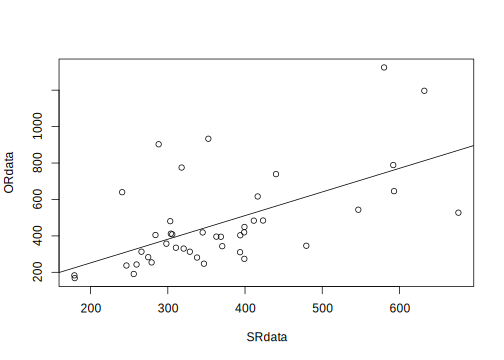
\includegraphics{Freq_CogSci_files/figure-latex/unnamed-chunk-71-1.pdf}

\begin{Shaded}
\begin{Highlighting}[]
\KeywordTok{cor}\NormalTok{(SRdata,ORdata)}
\end{Highlighting}
\end{Shaded}

\begin{verbatim}
## [1] 0.5876
\end{verbatim}

Returning to the t-test, by aggregating the data the independence assumption of the t-test is met, and the degrees of freedom for this by-subjects analysis are now correct (\(42-1=41\)):

\begin{Shaded}
\begin{Highlighting}[]
\KeywordTok{t.test}\NormalTok{(rawRT}\OperatorTok{~}\NormalTok{condition, bysubj,}\DataTypeTok{paired=}\OtherTok{TRUE}\NormalTok{)}
\end{Highlighting}
\end{Shaded}

\begin{verbatim}
## 
##  Paired t-test
## 
## data:  rawRT by condition
## t = 3.1, df = 41, p-value = 0.003
## alternative hypothesis: true difference in means is not equal to 0
## 95 percent confidence interval:
##   35.85 168.72
## sample estimates:
## mean of the differences 
##                   102.3
\end{verbatim}

Similar to the by-subjects aggregation done above, one could do a by-items aggregation and then a by-items t-test (What should be the degrees of freedom for the by-items analysis? There are 16 items in this data-set). This is left as an exercise for the reader.

The paired t-test illustrated above is actually not the best way to analyze this data-set, because it ignores the fact that each subject delivers not one but eight data points per condition. Each subject's repeated measurements will introduce a source of variance, but this source of variance is being suppressed in this t-test, leading to a possibly over-enthusiastic t-value. In order to take this variability into account, we must switch to the linear mixed model. But before we get to the linear mixed model, we have to consider the linear model. The next chapter turns to this topic.

\hypertarget{sec:SamplingDistrnexercises}{%
\section{Exercises}\label{sec:SamplingDistrnexercises}}

\hypertarget{sec:SamplingDistrnexercisesqt}{%
\subsection{\texorpdfstring{Practice using \texttt{qt}}{Practice using qt}}\label{sec:SamplingDistrnexercisesqt}}

Take an independent random sample of size \texttt{142} from a normal distribution
with mean \texttt{123}, and standard deviation \texttt{70}. Next, we are going to pretend we don't know the population parameters (the mean and standard deviation). We compute the MLEs of the mean and standard deviation using the data and get the sample mean \texttt{145.242} and the sample standard deviation \texttt{50.885}.

\begin{itemize}
\tightlist
\item
  Compute the estimated standard error using the sample standard deviation provided above.
\item
  What are your degrees of freedom for the relevant t-distribution?
\item
  Calculate the \textbf{absolute} critical t-value for a 95\% confidence interval using the relevant degrees of freedom you just wrote above.
\item
  Next, compute the lower bound of the 95\% confidence interval using the estimated standard error and the critical t-value.
\item
  Finally, compute the upper bound of the 95\% confidence interval using the estimated standard error and the critical t-value.
\end{itemize}

\hypertarget{sec:SamplingDistrnexercisesPart1}{%
\subsection{Computing the p-value}\label{sec:SamplingDistrnexercisesPart1}}

A paired t-test is done with data from 10 participants. The t-value from the test is 2.1. What is the p-value associated with a two-sided null hypothesis test?

\hypertarget{sec:SamplingDistrnexercisesPart2}{%
\subsection{Computing the t-value}\label{sec:SamplingDistrnexercisesPart2}}

If the p-value from a two-sided null hypothesis test had been 0.09, what would be the associated absolute t-value (i.e., ignoring the sign on the t-value)? The number of participants is 10, as above.

\hypertarget{sec:SamplingDistrnexercisesPart3}{%
\subsection{Type I and II error}\label{sec:SamplingDistrnexercisesPart3}}

Given that Type I error is 0.01; what is the highest value possible for Type II error?

\hypertarget{practice-with-the-paired-t-test}{%
\subsection{Practice with the paired t-test}\label{practice-with-the-paired-t-test}}

In a self-paced reading study, \citet{grodner} investigated subjects vs.~object relative clauses. They analyzed the reading times at the relative clause verb. However, a reviewer objects that the whole sentence's reading times (total reading times) should be used to evaluate the difference between the two conditions, because one cannot know where the difficulty might arise. It isn't clear whether one should use mean reading times over the entire sentence, or total reading times (summing up all the reading times over the entire sentence).
Carry out a by-subjects paired t-test on (a) the critical relative clause verb, versus (b) mean reading time over all words in the two sentence types, and (c) total reading times over all words in the two sentence types. Compare the t-value across the three tests, and decide what the appropriate dependent variable might be (Note: there is no correct answer here).

The data are loaded and pre-processed as follows. The code below gives you the reading times for the critical verb. You will have to work out how to obtain mean or total reading times for the whole sentence in each condition.

\begin{Shaded}
\begin{Highlighting}[]
\CommentTok{## load data:}
\KeywordTok{library}\NormalTok{(dplyr)}
\NormalTok{gg05e1 <-}\StringTok{ }\KeywordTok{read.table}\NormalTok{(}\StringTok{"data/GrodnerGibson2005E1.csv"}\NormalTok{,}\DataTypeTok{sep=}\StringTok{","}\NormalTok{, }
                     \DataTypeTok{header=}\OtherTok{TRUE}\NormalTok{)}
\NormalTok{gge1 <-}\StringTok{ }\NormalTok{gg05e1 }\OperatorTok\StringTok{ }
\StringTok{  }\KeywordTok{filter}\NormalTok{(item }\OperatorTok{!=}\StringTok{ }\DecValTok{0}\NormalTok{)}

\NormalTok{gge1 <-}\StringTok{ }\NormalTok{gge1 }\OperatorTok\StringTok{ }\KeywordTok{mutate}\NormalTok{(}\DataTypeTok{word_positionnew =} \KeywordTok{ifelse}\NormalTok{(item }\OperatorTok{!=}\StringTok{ }\DecValTok{15} \OperatorTok{&}\StringTok{ }
\StringTok{                                                    }\NormalTok{word_position }\OperatorTok{>}\StringTok{ }\DecValTok{10}\NormalTok{,}
\NormalTok{                                                  word_position}\DecValTok{-1}\NormalTok{, word_position)) }
\CommentTok{#there is a mistake in the coding of word position,}
\CommentTok{#all items but 15 have regions 10 and higher coded}
\CommentTok{#as words 11 and higher}

\CommentTok{## get data from relative clause verb:}
\NormalTok{gge1crit <-}\StringTok{ }\KeywordTok{subset}\NormalTok{(gge1, ( condition }\OperatorTok{==}\StringTok{ "objgap"} \OperatorTok{&}\StringTok{ }
\StringTok{                             }\NormalTok{word_position }\OperatorTok{==}\StringTok{ }\DecValTok{6}\NormalTok{ ) }\OperatorTok{|}
\StringTok{            }\NormalTok{( condition }\OperatorTok{==}\StringTok{ "subjgap"} \OperatorTok{&}\StringTok{ }\NormalTok{word_position }\OperatorTok{==}\StringTok{ }\DecValTok{4}\NormalTok{ ))}
\end{Highlighting}
\end{Shaded}

\hypertarget{linear-models-and-linear-mixed-models}{%
\chapter{Linear models and linear mixed models}\label{linear-models-and-linear-mixed-models}}

\hypertarget{from-the-t-test-to-the-linear-mixed-model}{%
\section{From the t-test to the linear (mixed) model}\label{from-the-t-test-to-the-linear-mixed-model}}

We begin with the \citet{grodner} self-paced reading data we saw in the previous chapter. Load the data and compute the means for the raw reading times by condition:

\begin{Shaded}
\begin{Highlighting}[]
\NormalTok{gg05e1<-}\KeywordTok{read.table}\NormalTok{(}\StringTok{"data/grodnergibsonE1crit.txt"}\NormalTok{,}
                   \DataTypeTok{header=}\OtherTok{TRUE}\NormalTok{)}
\NormalTok{means<-}\KeywordTok{round}\NormalTok{(}\KeywordTok{with}\NormalTok{(gg05e1,}\KeywordTok{tapply}\NormalTok{(rawRT,}
                                \DataTypeTok{IND=}\NormalTok{condition,}
\NormalTok{                            mean)))}
\NormalTok{means}
\end{Highlighting}
\end{Shaded}

\begin{verbatim}
##  objgap subjgap 
##     471     369
\end{verbatim}

As predicted by theory \citep{grodner}, object relatives (labeled objgap here) are read slower than subject relatives (labeled subjgap).

As discussed in the previous chapter, a paired t-test can be done to evaluate whether we have evidence against the null hypothesis that object relatives and subject relatives have identical reading times. However, we have to aggregate the data by subjects and by items first.

\begin{Shaded}
\begin{Highlighting}[]
\NormalTok{bysubj<-}\KeywordTok{aggregate}\NormalTok{(rawRT}\OperatorTok{~}\NormalTok{subject}\OperatorTok{+}
\StringTok{                    }\NormalTok{condition,}
\NormalTok{                  mean,}\DataTypeTok{data=}\NormalTok{gg05e1)}
\NormalTok{byitem<-}\KeywordTok{aggregate}\NormalTok{(rawRT}\OperatorTok{~}\NormalTok{item}\OperatorTok{+}
\StringTok{                    }\NormalTok{condition,}
\NormalTok{                  mean,}\DataTypeTok{data=}\NormalTok{gg05e1)}
\KeywordTok{t.test}\NormalTok{(rawRT}\OperatorTok{~}\NormalTok{condition,}
       \DataTypeTok{paired=}\OtherTok{TRUE}\NormalTok{,bysubj)}\OperatorTok{$}\NormalTok{statistic}
\end{Highlighting}
\end{Shaded}

\begin{verbatim}
##     t 
## 3.109
\end{verbatim}

\begin{Shaded}
\begin{Highlighting}[]
\KeywordTok{t.test}\NormalTok{(rawRT}\OperatorTok{~}\NormalTok{condition,}
       \DataTypeTok{paired=}\OtherTok{TRUE}\NormalTok{,byitem)}\OperatorTok{$}\NormalTok{statistic}
\end{Highlighting}
\end{Shaded}

\begin{verbatim}
##     t 
## 3.754
\end{verbatim}

What these two t-tests show is that both by subjects and by items, there is strong evidence against the null hypothesis that the object and relatives have identical reading times.

Interestingly, exactly the same t-values can be obtained by running the following commands, which implement a kind of linear model called the \emph{linear mixed model}:

\begin{Shaded}
\begin{Highlighting}[]
\KeywordTok{library}\NormalTok{(lme4)}
\end{Highlighting}
\end{Shaded}

\begin{verbatim}
## Loading required package: Matrix
\end{verbatim}

\begin{verbatim}
## 
## Attaching package: 'Matrix'
\end{verbatim}

\begin{verbatim}
## The following objects are masked from 'package:tidyr':
## 
##     expand, pack, unpack
\end{verbatim}

\begin{verbatim}
## 
## Attaching package: 'lme4'
\end{verbatim}

\begin{verbatim}
## The following object is masked from 'package:SIN':
## 
##     sdcor2cov
\end{verbatim}

\begin{Shaded}
\begin{Highlighting}[]
\NormalTok{m0lmersubj<-}\KeywordTok{lmer}\NormalTok{(rawRT}\OperatorTok{~}\NormalTok{condition}\OperatorTok{+}\NormalTok{(}\DecValTok{1}\OperatorTok{|}\NormalTok{subject),bysubj)}
\KeywordTok{summary}\NormalTok{(m0lmersubj)}\OperatorTok{$}\NormalTok{coefficients}
\end{Highlighting}
\end{Shaded}

\begin{verbatim}
##                  Estimate Std. Error t value
## (Intercept)         471.4      31.13  15.143
## conditionsubjgap   -102.3      32.90  -3.109
\end{verbatim}

\begin{Shaded}
\begin{Highlighting}[]
\NormalTok{m0lmeritem<-}\KeywordTok{lmer}\NormalTok{(rawRT}\OperatorTok{~}\NormalTok{condition}\OperatorTok{+}\NormalTok{(}\DecValTok{1}\OperatorTok{|}\NormalTok{item),byitem)}
\KeywordTok{summary}\NormalTok{(m0lmeritem)}\OperatorTok{$}\NormalTok{coefficients}
\end{Highlighting}
\end{Shaded}

\begin{verbatim}
##                  Estimate Std. Error t value
## (Intercept)         471.4      20.20  23.336
## conditionsubjgap   -102.3      27.25  -3.754
\end{verbatim}

The signs of the t-values are the opposite to that of the paired t-tests above; the reason for that will presently become clear.

Our goal in this chapter is to understand the above model involving the \texttt{lmer} function, using the familiar paired t-test as a starting point.

For now, consider only the by-subject analysis.
Given the sample means shown above for the two conditions,
we can rewrite our best guess about how the object and subject relative clause reading time distributions were generated:

\begin{itemize}
\tightlist
\item
  Object relative: \(Normal(471,\hat\sigma)\)
\item
  Subject relative: \(Normal(369,\hat\sigma)\)
\end{itemize}

This can also be rewritten with respect to the object relative mean and the difference between the two conditions (the reasons for this will become clear presently):

\begin{itemize}
\tightlist
\item
  Object relative: \(Normal(471-102\times 0,\hat\sigma)\)
\item
  Subject relative: \(Normal(471-102\times 1,\hat\sigma)\)
\end{itemize}

Note that the two distributions for object and subject relative clauses (RCs) are assumed to be independent. This assumed independence is expressed by the fact that we define two separate Normal distributions, one for object relatives and the other for subject relatives. We saw earlier that this assumption of independence does not hold in our data, because we have one data point for each RC type from the same subject. However, for now we will ignore this detail; we will fix this shortcoming later.

The interesting point to notice here is that the mean for the object and subject relatives' distributions can be rewritten as a sum of two terms. A completely equivalent way to express the fact that object relatives are coming from a \(Normal(471,\hat\sigma)\) is to say that each object relative data-point can be described by the following equation:

\begin{equation}
y = 471 + -102 \times 0 + \varepsilon \hfill \hbox{ where } \varepsilon \sim Normal(0,\hat\sigma)
\end{equation}

Similarly, the subject relative's distribution can be written as being generated from:

\begin{equation}
y = 471 - 102 \times 1 + \varepsilon \hbox{ where } \varepsilon \sim Normal(0,\hat\sigma)
\end{equation}

In these data, the parameter \(\hat\sigma\) is estimated to be \(213\). How do we know what this estimate is? This parameter's estimate can be derived from the by-subjects t-test output above: The observed t-value is

\begin{equation}
obs.t= \frac{\bar{x}}{s/\sqrt{n}} 
\end{equation}

Solving for \(s\):

\begin{equation}
 s = \bar{x} \times \sqrt{n}/obs.t = -102 \times \sqrt{42}/-3.109  =  213
\end{equation}

So, our model for the relative clause data consists of two equations:

Object relatives:

\begin{equation}
y = 471 -102\times 0 + \varepsilon \hfill \hbox{ where } \varepsilon \sim Normal(0,213)
\end{equation}

Subject relatives:

\begin{equation}
y = 471 - 102\times 1 + \varepsilon \hbox{ where } \varepsilon \sim Normal(0,213)
\end{equation}

The above statements describe a \emph{generative process} for the data.

Given such a statement about the generative process, we can express the estimated mean reading times for each RC type as follows. We can ignore the term \(\varepsilon\) because it has mean 0 (we stipulate this when we specify that \(\varepsilon \sim Normal(0,\sigma)\)).

Mean object relative reading times:

\begin{equation}
\hbox{Mean OR RT}= 471 -102\times 0
\end{equation}

Mean subject relative reading times:

\begin{equation}
\hbox{Mean SR RT} = 471 - 102\times 1 
\end{equation}

There is a function in R, the \texttt{lm()} function, which expresses the above statistical model, and prints out exactly the same numerical values that we used above:

\begin{Shaded}
\begin{Highlighting}[]
\KeywordTok{summary}\NormalTok{(m0<-}\KeywordTok{lm}\NormalTok{(rawRT}\OperatorTok{~}\NormalTok{condition,bysubj))}\OperatorTok{$}\NormalTok{coefficients}
\end{Highlighting}
\end{Shaded}

\begin{verbatim}
##                  Estimate Std. Error t value  Pr(>|t|)
## (Intercept)         471.4      31.13  15.143 1.795e-25
## conditionsubjgap   -102.3      44.02  -2.324 2.263e-02
\end{verbatim}

The linear model function \texttt{lm()} prints out two coefficients, \(471\) and \(-102\), that help express the mean reading times for object and subject relative data, using a simple coding scheme: object relatives are coded as 0, and subject relatives are coded as 1. This coding scheme is not visible to the user, but is represented internally in R. The user can see the coding for each condition level by typing:

\begin{Shaded}
\begin{Highlighting}[]
\CommentTok{## make sure that the condition column is of type factor:}
\NormalTok{bysubj}\OperatorTok{$}\NormalTok{condition<-}\KeywordTok{factor}\NormalTok{(bysubj}\OperatorTok{$}\NormalTok{condition)}
\KeywordTok{contrasts}\NormalTok{(bysubj}\OperatorTok{$}\NormalTok{condition)}
\end{Highlighting}
\end{Shaded}

\begin{verbatim}
##         subjgap
## objgap        0
## subjgap       1
\end{verbatim}

We will discuss contrast coding in detail in a later chapter, but right now the simple 0,1 coding above---called treatment contrasts---is enough for our purposes.

Thus, what the linear model above gives us is two numbers: the mean object relative reading time (471), and the \emph{difference} between object and subject relative (-102). We can extract the two coefficients by typing:

\begin{Shaded}
\begin{Highlighting}[]
\KeywordTok{round}\NormalTok{(}\KeywordTok{coef}\NormalTok{(m0))}
\end{Highlighting}
\end{Shaded}

\begin{verbatim}
##      (Intercept) conditionsubjgap 
##              471             -102
\end{verbatim}

In the vocabulary of linear modeling, the first number is called the \emph{intercept}, and the second one is called the \emph{slope}.
Note that the meaning of the intercept and slope depends on the ordering of the factor levels. We can make the sample mean of the subject relative represent the intercept:

\begin{Shaded}
\begin{Highlighting}[]
\CommentTok{## reverse the factor level ordering:}
\NormalTok{bysubj}\OperatorTok{$}\NormalTok{condition<-}\KeywordTok{factor}\NormalTok{(bysubj}\OperatorTok{$}\NormalTok{condition,}
                         \DataTypeTok{levels=}\KeywordTok{c}\NormalTok{(}\StringTok{"subjgap"}\NormalTok{,}\StringTok{"objgap"}\NormalTok{))}
\KeywordTok{contrasts}\NormalTok{(bysubj}\OperatorTok{$}\NormalTok{condition)}
\end{Highlighting}
\end{Shaded}

\begin{verbatim}
##         objgap
## subjgap      0
## objgap       1
\end{verbatim}

Now, the intercept is the mean of the subject relatives, and the slope is the difference between object and subject relatives reading times. Note that the sign of the t-value has changed---the sign depends on the contrast coding.

\begin{Shaded}
\begin{Highlighting}[]
\NormalTok{m1a<-}\KeywordTok{lm}\NormalTok{(rawRT}\OperatorTok{~}\NormalTok{condition,bysubj)}
\KeywordTok{summary}\NormalTok{(m1a)}\OperatorTok{$}\NormalTok{coefficients}
\end{Highlighting}
\end{Shaded}

\begin{verbatim}
##                 Estimate Std. Error t value  Pr(>|t|)
## (Intercept)        369.1      31.13  11.857 1.819e-19
## conditionobjgap    102.3      44.02   2.324 2.263e-02
\end{verbatim}

Let's switch back to the original factor level ordering:

\begin{Shaded}
\begin{Highlighting}[]
\NormalTok{bysubj}\OperatorTok{$}\NormalTok{condition<-}\KeywordTok{factor}\NormalTok{(bysubj}\OperatorTok{$}\NormalTok{condition,}
                         \DataTypeTok{levels=}\KeywordTok{c}\NormalTok{(}\StringTok{"objgap"}\NormalTok{,}\StringTok{"subjgap"}\NormalTok{))}
\KeywordTok{contrasts}\NormalTok{(bysubj}\OperatorTok{$}\NormalTok{condition)}
\end{Highlighting}
\end{Shaded}

\begin{verbatim}
##         subjgap
## objgap        0
## subjgap       1
\end{verbatim}

In mathematical form, the model can now be stated as a single equation:

\begin{equation}
rawRT = \beta_0 + \beta_1 condition + \varepsilon
\end{equation}

where

\begin{itemize}
\tightlist
\item
  condition is a 0,1 coded vector, with object relatives coded as 0, and subject relatives coded as 1.
\item
  \(\beta_0\) is the mean for the object relative (which is coded as 0)
\item
  \(\beta_1\) is the amount by which the object relative mean must be
  changed to obtain the mean for the subject relative.
\item
  \(\varepsilon\) is the noisy variation from trial to trial around the means for the two conditions, represented by \(Normal(0,213)\).
\end{itemize}

The null hypothesis of scientific interest here is always with reference to the slope, that the difference in means between the two relative clause types \(\beta_1\) is:

\(H_0: \beta_1 = 0\)

The t-test value printed out in the linear model is simply the familiar t-test formula in action:

\begin{equation}
obs.t = \frac{\beta_1 - 0}{SE}
\end{equation}

The intercept also has a null hypothesis associated with it, namely that
\(H_0: \beta_0 = 0\). However, this null hypothesis test is of absolutely no interest for us. This hypothesis test is reported by the lm() function only because the intercept is needed for technical reasons, to be discussed later.

The \emph{contrast coding} mentioned above determines the meaning of the \(\beta\) parameters:

\begin{Shaded}
\begin{Highlighting}[]
\NormalTok{bysubj}\OperatorTok{$}\NormalTok{condition<-}\KeywordTok{factor}\NormalTok{(bysubj}\OperatorTok{$}\NormalTok{condition,}
                         \DataTypeTok{levels=}\KeywordTok{c}\NormalTok{(}\StringTok{"objgap"}\NormalTok{,}\StringTok{"subjgap"}\NormalTok{))}
\KeywordTok{contrasts}\NormalTok{(bysubj}\OperatorTok{$}\NormalTok{condition)}
\end{Highlighting}
\end{Shaded}

\begin{verbatim}
##         subjgap
## objgap        0
## subjgap       1
\end{verbatim}

When discussing linear models, we will make a distinction between the unknown true means \(\beta_0, \beta_1\) and the estimated mean from the data \(\hat\beta_0, \hat\beta_1\). The estimates that we have from the data are:

\begin{itemize}
\tightlist
\item
  Estimated mean object relative processing time: \(\hat\beta_0=471\)
  .
\item
  Estimated mean subject relative processing time: \(\hat\beta_0+\hat\beta_1=471+-102=369\).
\end{itemize}

\hypertarget{sum-coding}{%
\section{Sum coding}\label{sum-coding}}

We have established so far that the mathematical form of the model is:

\begin{equation}
rawRT = \beta_0 + \beta_1 condition + \varepsilon
\end{equation}

We can change the contrast coding of the \texttt{condition} vector in the following way. First, recode the levels of the condition column as shown below.

\begin{Shaded}
\begin{Highlighting}[]
\CommentTok{## new contrast coding:}
\NormalTok{bysubj}\OperatorTok{$}\NormalTok{cond<-}\KeywordTok{ifelse}\NormalTok{(bysubj}\OperatorTok{$}\NormalTok{condition}\OperatorTok{==}\StringTok{"objgap"}\NormalTok{,}\DecValTok{1}\NormalTok{,}\OperatorTok{-}\DecValTok{1}\NormalTok{)}
\end{Highlighting}
\end{Shaded}

Now, the two conditions are coded not as 0, 1 but as -1 and +1:

\begin{Shaded}
\begin{Highlighting}[]
\KeywordTok{xtabs}\NormalTok{(}\OperatorTok{~}\NormalTok{cond}\OperatorTok{+}\NormalTok{condition,bysubj)}
\end{Highlighting}
\end{Shaded}

\begin{verbatim}
##     condition
## cond objgap subjgap
##   -1      0      42
##   1      42       0
\end{verbatim}

With this coding, the model parameters have a different meaning:

\begin{Shaded}
\begin{Highlighting}[]
\NormalTok{m1<-}\KeywordTok{lm}\NormalTok{(rawRT}\OperatorTok{~}\NormalTok{cond,bysubj)}
\KeywordTok{round}\NormalTok{(}\KeywordTok{coef}\NormalTok{(m1))}
\end{Highlighting}
\end{Shaded}

\begin{verbatim}
## (Intercept)        cond 
##         420          51
\end{verbatim}

\begin{itemize}
\tightlist
\item
  The intercept now represents the grand mean processing time: \(\hat \beta_0=420\).
\item
  The mean object relative processing time is now: \(\hat\beta_0+\hat\beta_1\times 1=420+51=471\).
\item
  The mean subject relative processing time is: \(\hat\beta_0+\hat\beta_1\times (-1)=420-51=369\).
\end{itemize}

This kind of parameterization is called \emph{sum-to-zero contrast} or more simply \emph{sum contrast} coding. This is the coding we will use most frequently in this book. We will elaborate on contrast coding in a later chapter; there, the advantages of sum coding over treatment coding will become clear. For now, it is sufficient to understand that one can \emph{reparametrize} the model using different contrast codings, and that such a reparametrization impacts the interpretation of the parameters.

With sum coding, the null hypothesis for the slope is

\begin{equation}
H_0: \mathbf{1\times} \mu_{obj} + (\mathbf{-1}) \times\mu_{subj} = 0   
\end{equation}

The sum contrast coding of +1 standing for object relatives and -1 standing for subject relatives in the linear model directly refer to the \(\pm 1\) coefficients in the null hypothesis above.
Now the model is as follows.

Object relative reading times:

\begin{equation}
rt = 420\mathbf{\times 1} + 51\mathbf{\times 1} + \varepsilon
\end{equation}

Subject relative reading times:

\begin{equation}
rt = 420\mathbf{\times 1} + 51\mathbf{\times (-1)} + \varepsilon
\end{equation}

One could write it in a single line as:

\begin{equation}
rt = 420 + 51\times condition + \varepsilon
\end{equation}

The term \(\varepsilon\) is call the residuals; it is the amount by which the observed data deviate from the values predicted by the above model. For example, suppose that a data point for a subject relative condition is 400 ms. The model predicts a reading time of 420-51=369 ms. The residual for that data point would be 400-369= 31. Another example: suppose that a data point for an object relative condition is 200 ms. The model predicts the object relative to be 420+51=471. The residual for that data point would then be 200-471=-271. Thus, the residual is the amount of the discrepancy between the model's predicted reading time and the actually observed reading time.

\hypertarget{checking-model-assumptions}{%
\section{Checking model assumptions}\label{checking-model-assumptions}}

It is an assumption of the linear model that the residuals are (approximately) normally distributed, That is what the statement \(\varepsilon\sim Normal(0,\sigma)\) implies. It is important to check that model assumptions are approximately satisfied; this is because the null hypothesis significance testing procedure requires approximate normality of residuals.

Here is how we can check whether this normality assumption is met:

\begin{Shaded}
\begin{Highlighting}[]
\CommentTok{## extract residuals:}
\NormalTok{res.m1<-}\KeywordTok{residuals}\NormalTok{(m1)}
\end{Highlighting}
\end{Shaded}

Compare the residuals to the quantiles of the standard normal distribution (\(Normal(0,1)\)):

When the normality assumption is met, the residuals will align perfectly with the quantiles of the standard normal distribution, resulting in a straight diagonal line in the above plot. When the normality assumption is not met, the line will tend to curve away from the diagonal.

In the above case, a log transform of the data improves the normality of residuals. We will discuss transformation in detail later in this book; for now, it is sufficient to note that for continuous data that consists of all-positive values (here, reading times), a log transform will often be the appropriate transform.

\begin{Shaded}
\begin{Highlighting}[]
\NormalTok{m1log<-}\KeywordTok{lm}\NormalTok{(}\KeywordTok{log}\NormalTok{(rawRT)}\OperatorTok{~}\NormalTok{cond,bysubj)}
\KeywordTok{qqnorm}\NormalTok{(}\KeywordTok{residuals}\NormalTok{(m1log))}
\end{Highlighting}
\end{Shaded}

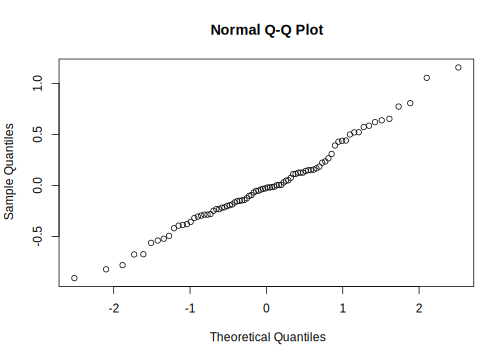
\includegraphics{Freq_CogSci_files/figure-latex/unnamed-chunk-91-1.pdf}

The estimates of the parameters are now in the log scale:

\begin{itemize}
\tightlist
\item
  The estimated grand mean processing time: \(\hat\beta_0=5.9488\).
\item
  The estimated mean object relative processing time: \(\hat\beta_0+\hat\beta_1=5.9488+0.0843=6.0331\).
\item
  The estimated mean subject relative processing time: \(\hat\beta_0-\hat\beta_1=5.9488-0.0843=5.8645\).
\end{itemize}

The model does not change, only the scale does:

\begin{equation}
\log rt = \beta_0 + \beta_1 condition  + \varepsilon 
\end{equation}

Now, the intercept and slope can be used to compute the reading time in the two conditions.
Note that because \(exp(log(rt))=rt\), to get the mean estimates on the raw ms scale, we just need to exponentiate both sides of the equation:

\begin{equation}
exp(\log rt) = exp( \beta_0 + \beta_1 condition)
\end{equation}

This approach gives us the following estimates on the ms scale:

\begin{itemize}
\tightlist
\item
  Estimated mean object relative reading time: \(exp(\hat\beta_0+\hat\beta_1)=exp(5.9488+0.0843)=417\).
\item
  Estimated mean subject relative reading time: \(exp(\hat\beta_0-\hat\beta_1)=exp(5.9488-0.0843=352\).
\end{itemize}

The difference in reading time is 417-352=65 ms. If we had fit the model to raw reading times, the difference would have been:

\begin{Shaded}
\begin{Highlighting}[]
\NormalTok{m1raw<-}\KeywordTok{lm}\NormalTok{(rawRT}\OperatorTok{~}\NormalTok{cond,bysubj)}
\end{Highlighting}
\end{Shaded}

\begin{itemize}
\tightlist
\item
  Estimated mean object relative reading time: \(\hat\beta_0+\hat\beta_1=420.22+51.14=471.36\).
\item
  Estimated mean subject relative reading time: \(\hat\beta_0-\hat\beta_1=420.22-51.14=369.08\).
\end{itemize}

The difference in the means on the raw scale is 102 ms.
The larger estimate based on the raw scale is less realistic, and we will see later that the large difference between the two conditions is driven by a few extreme, influential values.

\hypertarget{from-the-paired-t-test-to-the-linear-mixed-model}{%
\section{From the paired t-test to the linear mixed model}\label{from-the-paired-t-test-to-the-linear-mixed-model}}

One important point to notice is that the observed t-value of the paired t-test and the t-test printed out by the linear model don't match:

\begin{Shaded}
\begin{Highlighting}[]
\KeywordTok{t.test}\NormalTok{(rawRT}\OperatorTok{~}\NormalTok{condition,bysubj,}\DataTypeTok{paired=}\OtherTok{TRUE}\NormalTok{)}\OperatorTok{$}\NormalTok{statistic}
\end{Highlighting}
\end{Shaded}

\begin{verbatim}
##     t 
## 3.109
\end{verbatim}

\begin{Shaded}
\begin{Highlighting}[]
\KeywordTok{round}\NormalTok{(}\KeywordTok{summary}\NormalTok{(m0)}\OperatorTok{$}\NormalTok{coefficients,}\DecValTok{2}\NormalTok{)[,}\KeywordTok{c}\NormalTok{(}\DecValTok{1}\OperatorTok{:}\DecValTok{3}\NormalTok{)]}
\end{Highlighting}
\end{Shaded}

\begin{verbatim}
##                  Estimate Std. Error t value
## (Intercept)         471.4      31.13   15.14
## conditionsubjgap   -102.3      44.02   -2.32
\end{verbatim}

This is because the linear model is equivalent to the unpaired (i.e., two sample) t-test:

\begin{Shaded}
\begin{Highlighting}[]
\KeywordTok{summary}\NormalTok{(}\KeywordTok{lm}\NormalTok{(rawRT}\OperatorTok{~}\NormalTok{condition,bysubj))}
\end{Highlighting}
\end{Shaded}

\begin{verbatim}
## 
## Call:
## lm(formula = rawRT ~ condition, data = bysubj)
## 
## Residuals:
##    Min     1Q Median     3Q    Max 
## -303.4 -116.4  -51.6   49.1  853.3 
## 
## Coefficients:
##                  Estimate Std. Error t value Pr(>|t|)
## (Intercept)         471.4       31.1   15.14   <2e-16
## conditionsubjgap   -102.3       44.0   -2.32    0.023
## 
## Residual standard error: 202 on 82 degrees of freedom
## Multiple R-squared:  0.0618, Adjusted R-squared:  0.0503 
## F-statistic:  5.4 on 1 and 82 DF,  p-value: 0.0226
\end{verbatim}

\begin{Shaded}
\begin{Highlighting}[]
\KeywordTok{round}\NormalTok{(}\KeywordTok{t.test}\NormalTok{(rawRT}\OperatorTok{~}\NormalTok{condition,bysubj,}
             \DataTypeTok{paired=}\OtherTok{FALSE}\NormalTok{)}\OperatorTok{$}\NormalTok{statistic,}\DecValTok{2}\NormalTok{)}
\end{Highlighting}
\end{Shaded}

\begin{verbatim}
##    t 
## 2.32
\end{verbatim}

The paired t-test has an equivalent in the linear modeling framework: the linear mixed model. We turn next to this extension of the simple linear model. The command corresponding to the paired t-test in the linear modeling framework is:

\begin{Shaded}
\begin{Highlighting}[]
\NormalTok{m0.lmer<-}\KeywordTok{lmer}\NormalTok{(rawRT}\OperatorTok{~}\NormalTok{condition}\OperatorTok{+}\NormalTok{(}\DecValTok{1}\OperatorTok{|}\NormalTok{subject),bysubj)}
\KeywordTok{summary}\NormalTok{(m0.lmer)}\OperatorTok{$}\NormalTok{coefficients}
\end{Highlighting}
\end{Shaded}

\begin{verbatim}
##                  Estimate Std. Error t value
## (Intercept)         471.4      31.13  15.143
## conditionsubjgap   -102.3      32.90  -3.109
\end{verbatim}

To understand the connection between the paired t-test and the above command, it is necessary to consider how a paired t-test is assembled.

First, some background. If you have two random variables that have correlation \(\rho\), the variance of the difference between the two random variables is:

\begin{equation}
Var(X_1-X_2)=Var(X_1) + Var(X_2) - 2\times Cov(X_1, X_2)
\end{equation}

\(Cov(X_1, X2)\) is the covariance between the two random variables and is defined as:

\begin{equation}
Cov(X_1, X_2) = \rho \sqrt{Var(X_1)}\sqrt{Var(X_2)}
\end{equation}

You can find the proofs of the above assertions in books like \citet{rice1995mathematical}.

As discussed earlier, a paired t-test is used when you have paired data from subject \(i=1,...,n\) in two conditions, say conditions 1 and 2. Let's write the data as two vectors \(X_{1}, X_{2}\). Because the pairs of data points are coming from the same subject, they are correlated with some correlation \(\rho\). Assume that both conditions 1 and 2 have standard deviation \(\sigma\).

To make this discussion concrete, let's generate some simulated bivariate data that are correlated. Assume that \(\sigma = 1\),
\(\rho=0.5\), and that the data are balanced.

\begin{Shaded}
\begin{Highlighting}[]
\KeywordTok{library}\NormalTok{(MASS)}
\NormalTok{samplesize<-}\DecValTok{12}
\NormalTok{mu <-}\StringTok{ }\KeywordTok{c}\NormalTok{(.}\DecValTok{3}\NormalTok{, }\FloatTok{.2}\NormalTok{)}
\NormalTok{rho<-}\FloatTok{0.5}
\NormalTok{stddev<-}\DecValTok{1}
\NormalTok{Sigma <-}\StringTok{ }\KeywordTok{matrix}\NormalTok{(stddev, }\DataTypeTok{nrow=}\DecValTok{2}\NormalTok{, }\DataTypeTok{ncol=}\DecValTok{2}\NormalTok{) }\OperatorTok{+}\StringTok{ }\KeywordTok{diag}\NormalTok{(}\DecValTok{2}\NormalTok{)}
\NormalTok{Sigma<-Sigma}\OperatorTok{/}\DecValTok{2}
\NormalTok{Sigma}
\end{Highlighting}
\end{Shaded}

\begin{verbatim}
##      [,1] [,2]
## [1,]  1.0  0.5
## [2,]  0.5  1.0
\end{verbatim}

\begin{Shaded}
\begin{Highlighting}[]
\CommentTok{## simulated data:}
\NormalTok{x <-}\StringTok{ }\KeywordTok{mvrnorm}\NormalTok{(}\DataTypeTok{n=}\NormalTok{samplesize, }\DataTypeTok{mu=}\NormalTok{mu, }\DataTypeTok{Sigma=}\NormalTok{Sigma, }\DataTypeTok{empirical=}\OtherTok{TRUE}\NormalTok{)}
\KeywordTok{head}\NormalTok{(x)}
\end{Highlighting}
\end{Shaded}

\begin{verbatim}
##         [,1]    [,2]
## [1,] -0.5361  0.1271
## [2,]  1.3814  1.3024
## [3,] -0.7434 -0.1521
## [4,]  2.3506  0.3507
## [5,] -1.2914 -1.4430
## [6,]  0.1007 -0.9218
\end{verbatim}

\begin{Shaded}
\begin{Highlighting}[]
\NormalTok{n<-samplesize}
\NormalTok{x1<-x[,}\DecValTok{1}\NormalTok{]}
\NormalTok{x2<-x[,}\DecValTok{2}\NormalTok{]}
\NormalTok{x1}
\end{Highlighting}
\end{Shaded}

\begin{verbatim}
##  [1] -0.5361  1.3814 -0.7434  2.3506 -1.2914  0.1007
##  [7]  0.5587 -0.3438  0.5338 -0.0866  0.8119  0.8640
\end{verbatim}

\begin{Shaded}
\begin{Highlighting}[]
\NormalTok{x2}
\end{Highlighting}
\end{Shaded}

\begin{verbatim}
##  [1]  0.1271  1.3024 -0.1521  0.3507 -1.4430 -0.9218
##  [7]  0.3375 -0.3714 -0.8318  1.5399  1.6450  0.8175
\end{verbatim}

To carry out the paired t-test,
we need to know the variance of \(X_1-X_2\) because the t-statistic will be:

\begin{equation}
t_{n-1} = \frac{X_1 - X_2}{\sqrt{Var(X_1 - X_2)/n}}
\end{equation}

Now,

\begin{equation}
Var(X_1 - X_2) = \sigma^2 + \sigma^2 - 2 \rho \sigma\sigma = 2\sigma^2 (1-\rho)
\end{equation}

Now let's compute the t-statistic using the above formula. Let the actual data vectors be \(x_1, x_2\).

\begin{equation}
t_{n-1} = \frac{mean(x_1) - mean(x_2)}{\sqrt{Var(X_1 - X_2)/n}}
\end{equation}

This simplifies to:

\begin{equation}
t_{n-1} = \frac{mean(x_1) - mean(x_2)}{\sqrt{2\sigma^2(1-\rho)/n}}
\end{equation}

Now compare the paired t-test output and the by-hand calculation:

\begin{Shaded}
\begin{Highlighting}[]
\KeywordTok{t.test}\NormalTok{(x1,x2,}\DataTypeTok{paired=}\OtherTok{TRUE}\NormalTok{)}\OperatorTok{$}\NormalTok{statistic}
\end{Highlighting}
\end{Shaded}

\begin{verbatim}
##      t 
## 0.3464
\end{verbatim}

\begin{Shaded}
\begin{Highlighting}[]
\NormalTok{(}\KeywordTok{mean}\NormalTok{(x1)}\OperatorTok{-}\KeywordTok{mean}\NormalTok{(x2))}\OperatorTok{/}\KeywordTok{sqrt}\NormalTok{((}\DecValTok{2}\OperatorTok{*}\NormalTok{stddev}\OperatorTok{^}\DecValTok{2}\OperatorTok{*}\NormalTok{(}\DecValTok{1}\OperatorTok{-}\NormalTok{rho))}\OperatorTok{/}\NormalTok{n)}
\end{Highlighting}
\end{Shaded}

\begin{verbatim}
## [1] 0.3464
\end{verbatim}

The linear mixed model we present next will fit exactly the same model as in the paired t-test above. To see this, suppose we have \(i\) subjects and \(j=1,2\) conditions. For simplicity, assume that each subject sees each condition once (e.g., the by-subjects aggregated English relative clause data), so we have two data points from each subject. In other words, the data are paired.

Then, for condition 1, the dependent variable can be described by the equation:

\(y_{i1} = \beta_0 + u_i + \varepsilon_{i1}\)

Here, \(\beta_0\) is the mean reading time, and \(\varepsilon\) is the usual residual error term. The interesting new term is \(u_i\). This is the adjustment to the mean reading time for subject \(i\). That is, if some subject is slower than average, \(u_i\) will be a positive number; if a subject is faster than average, then that subject's adjustment \(u_i\) will be negative in sign; and if a subject has exactly the same reading time as the mean for all subjects, then \(u_i\) for that subject will be 0.

Similarly, for condition 2, the dependent variable is described by the equation:

\(y_{i2} = \beta_0 + \delta + u_i + \varepsilon_{i2}\)

Here, \(\delta\) is the additional time taken to process condition 2 (thus, this is the treatment contrast coding we saw earlier in this chapter).

If we subtract the equation for condition 2 from the equation for condition 1, the resulting equation is:

\(d_i=y_{i1} - y_{i2}= \delta + (\varepsilon_{i1}-\varepsilon_{i2})\)

The expectation of \(d_i\) is \(\delta\) because the expectation of the \(\varepsilon\) terms is 0 (we set up the model such that \(\varepsilon \sim Normal(0,\sigma)\)).

Now, assuming that the error terms are correlated with correlation \(\rho\), the result presented at the beginning of this section applies:

\begin{equation}
Var(y_{i1}-y_{i2}) = \sigma^2 + \sigma^2-2\rho\sigma^2=2\sigma^2(1-\rho)
\end{equation}

The generative distribution for \(d_i\), the pairwise differences in the two conditions, is

\begin{equation}
d \sim Normal(\delta, \sqrt{2\sigma^2(1-\rho)})
\end{equation}

But that is exactly the same standard deviation as the one used in the paired t-test.

So, the paired t-test will deliver exactly the same t-score as the above linear mixed model.

Let's check that this is true using our simulated data. In the code below, the term \texttt{(1\textbar{}subj)} is the adjustment by subject to the intercepts---the term \(u0_i\) above.

\begin{Shaded}
\begin{Highlighting}[]
\KeywordTok{library}\NormalTok{(lme4)}
\NormalTok{dat<-}\KeywordTok{data.frame}\NormalTok{(}\DataTypeTok{y=}\KeywordTok{c}\NormalTok{(x1,x2),}\DataTypeTok{cond=}\KeywordTok{rep}\NormalTok{(letters[}\DecValTok{1}\OperatorTok{:}\DecValTok{2}\NormalTok{],}\DataTypeTok{each=}\NormalTok{n),}\DataTypeTok{subj=}\KeywordTok{rep}\NormalTok{(}\DecValTok{1}\OperatorTok{:}\NormalTok{n,}\DecValTok{2}\NormalTok{))}
\NormalTok{dat}\OperatorTok{$}\NormalTok{cond<-}\KeywordTok{factor}\NormalTok{(dat}\OperatorTok{$}\NormalTok{cond)}
\KeywordTok{contrasts}\NormalTok{(dat}\OperatorTok{$}\NormalTok{cond)<-}\KeywordTok{contr.sum}\NormalTok{(}\DecValTok{2}\NormalTok{)}
\KeywordTok{contrasts}\NormalTok{(dat}\OperatorTok{$}\NormalTok{cond)}
\end{Highlighting}
\end{Shaded}

\begin{verbatim}
##   [,1]
## a    1
## b   -1
\end{verbatim}

\begin{Shaded}
\begin{Highlighting}[]
\KeywordTok{summary}\NormalTok{(m<-}\KeywordTok{lmer}\NormalTok{(y}\OperatorTok{~}\NormalTok{cond}\OperatorTok{+}\NormalTok{(}\DecValTok{1}\OperatorTok{|}\NormalTok{subj),dat))}
\end{Highlighting}
\end{Shaded}

\begin{verbatim}
## Linear mixed model fit by REML ['lmerMod']
## Formula: y ~ cond + (1 | subj)
##    Data: dat
## 
## REML criterion at convergence: 65.6
## 
## Scaled residuals: 
##     Min      1Q  Median      3Q     Max 
## -1.0830 -0.7651  0.0838  0.3807  1.8623 
## 
## Random effects:
##  Groups   Name        Variance Std.Dev.
##  subj     (Intercept) 0.5      0.707   
##  Residual             0.5      0.707   
## Number of obs: 24, groups:  subj, 12
## 
## Fixed effects:
##             Estimate Std. Error t value
## (Intercept)    0.250      0.250    1.00
## cond1          0.050      0.144    0.35
## 
## Correlation of Fixed Effects:
##       (Intr)
## cond1 0.000
\end{verbatim}

The t-statistic from the linear mixed model is exactly the same as that from the paired t-test.

With this as background, we are ready to look at linear mixed models in detail.

\hypertarget{linear-mixed-models}{%
\section{Linear mixed models}\label{linear-mixed-models}}

We return to our subject and object relative clause data from English (Grodner and Gibson, Expt 1). First we load the data as usual, define relative clause type as a sum coded predictor, and create a new column called \texttt{so} that represents the contrast coding (\(\pm 1\) sum contrasts), and a column that holds log-transformed reading time.

\begin{Shaded}
\begin{Highlighting}[]
\NormalTok{gg05e1<-}\KeywordTok{read.table}\NormalTok{(}\StringTok{"data/grodnergibsonE1crit.txt"}\NormalTok{,}\DataTypeTok{header=}\OtherTok{TRUE}\NormalTok{)}

\NormalTok{gg05e1}\OperatorTok{$}\NormalTok{so <-}\StringTok{ }\KeywordTok{ifelse}\NormalTok{(gg05e1}\OperatorTok{$}\NormalTok{condition}\OperatorTok{==}\StringTok{"objgap"}\NormalTok{,}\DecValTok{1}\NormalTok{,}\OperatorTok{-}\DecValTok{1}\NormalTok{)}
\NormalTok{gg05e1}\OperatorTok{$}\NormalTok{logrt<-}\KeywordTok{log}\NormalTok{(gg05e1}\OperatorTok{$}\NormalTok{rawRT)}
\end{Highlighting}
\end{Shaded}

Recall that these data have multiple measurements from each subject for each condition:

\begin{Shaded}
\begin{Highlighting}[]
\KeywordTok{t}\NormalTok{(}\KeywordTok{xtabs}\NormalTok{(}\OperatorTok{~}\NormalTok{subject}\OperatorTok{+}\NormalTok{condition, gg05e1))}
\end{Highlighting}
\end{Shaded}

\begin{verbatim}
##          subject
## condition 1 2 3 4 5 6 7 8 9 10 11 12 13 14 15 16 17 18
##   objgap  8 8 8 8 8 8 8 8 8  8  8  8  8  8  8  8  8  8
##   subjgap 8 8 8 8 8 8 8 8 8  8  8  8  8  8  8  8  8  8
##          subject
## condition 19 20 21 22 23 24 25 26 27 28 29 30 31 32 33
##   objgap   8  8  8  8  8  8  8  8  8  8  8  8  8  8  8
##   subjgap  8  8  8  8  8  8  8  8  8  8  8  8  8  8  8
##          subject
## condition 34 35 36 37 38 39 40 41 42
##   objgap   8  8  8  8  8  8  8  8  8
##   subjgap  8  8  8  8  8  8  8  8  8
\end{verbatim}

We can visualize the different responses of subjects:

\begin{verbatim}
## `geom_smooth()` using formula 'y ~ x'
\end{verbatim}

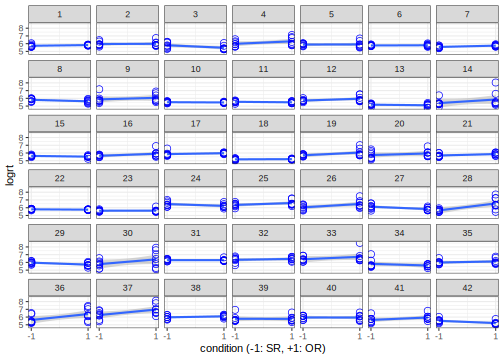
\includegraphics{Freq_CogSci_files/figure-latex/unnamed-chunk-101-1.pdf}

It's clear that different subjects have different effects of the relative clause manipulation: some slopes are positive sloping, some are flat, and some are negatively sloping. There is between-subject variability in the relative clause effect.

Given these differences between subjects, you could fit a separate linear model for each subject, collect together the intercepts and slopes for each subject, and then check if the slopes are significantly different from zero. There is a function in the package \texttt{lme4} that computes separate linear models for each subject: \emph{lmList}.

\begin{Shaded}
\begin{Highlighting}[]
\KeywordTok{library}\NormalTok{(lme4)}

\NormalTok{lmlist.fm1<-}\KeywordTok{lmList}\NormalTok{(logrt}\OperatorTok{~}\NormalTok{so}\OperatorTok{|}\NormalTok{subject,gg05e1)}
\end{Highlighting}
\end{Shaded}

One can extract the intercept and slope estimates for each subject. For example, for subject 1:

\begin{Shaded}
\begin{Highlighting}[]
\NormalTok{lmlist.fm1}\OperatorTok{$}\StringTok{`}\DataTypeTok{1}\StringTok{`}\OperatorTok{$}\NormalTok{coefficients}
\end{Highlighting}
\end{Shaded}

\begin{verbatim}
## (Intercept)          so 
##     5.76962     0.04352
\end{verbatim}

One can plot the individual lines for each subject, as well as the fit of a simple linear model m0 for all the data taken together; this will show how each subject deviates in intercept and slope from the model m0's intercept and slope.

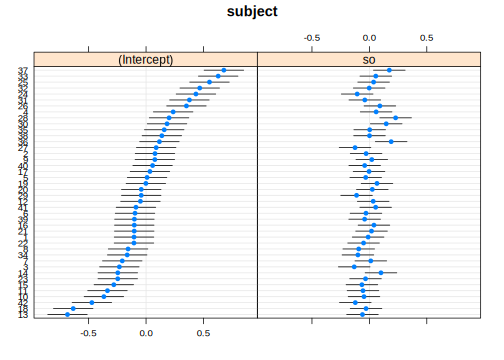
\includegraphics{Freq_CogSci_files/figure-latex/unnamed-chunk-104-1.pdf}

To find out if there is an effect of relative clause type, we simply need to check whether the slopes of the individual subjects' fitted lines taken together are significantly different from zero. A one-sample t-test will achieve this:

\begin{Shaded}
\begin{Highlighting}[]
\KeywordTok{t.test}\NormalTok{(}\KeywordTok{coef}\NormalTok{(lmlist.fm1)[}\DecValTok{2}\NormalTok{])}
\end{Highlighting}
\end{Shaded}

\begin{verbatim}
## 
##  One Sample t-test
## 
## data:  coef(lmlist.fm1)[2]
## t = 2.8, df = 41, p-value = 0.008
## alternative hypothesis: true mean is not equal to 0
## 95 percent confidence interval:
##  0.01745 0.10658
## sample estimates:
## mean of x 
##   0.06202
\end{verbatim}

The above test is \emph{exactly} the same as the paired t-test and the varying intercepts linear mixed model that we fit in the last chapter using the by-subject aggregated data:

\begin{Shaded}
\begin{Highlighting}[]
\NormalTok{bysubj<-}\KeywordTok{aggregate}\NormalTok{(}\KeywordTok{log}\NormalTok{(rawRT)}\OperatorTok{~}\NormalTok{subject}\OperatorTok{+}\NormalTok{condition,}
\NormalTok{                  mean,}\DataTypeTok{data=}\NormalTok{gg05e1)}

\KeywordTok{colnames}\NormalTok{(bysubj)[}\DecValTok{3}\NormalTok{]<-}\StringTok{"logrt"}

\KeywordTok{t.test}\NormalTok{(logrt}\OperatorTok{~}\NormalTok{condition,bysubj,}\DataTypeTok{paired=}\OtherTok{TRUE}\NormalTok{)}\OperatorTok{$}\NormalTok{statistic}
\end{Highlighting}
\end{Shaded}

\begin{verbatim}
##    t 
## 2.81
\end{verbatim}

\begin{Shaded}
\begin{Highlighting}[]
\CommentTok{## compare with linear mixed model:}
\KeywordTok{summary}\NormalTok{(}\KeywordTok{lmer}\NormalTok{(logrt}\OperatorTok{~}\NormalTok{condition}\OperatorTok{+}\NormalTok{(}\DecValTok{1}\OperatorTok{|}\NormalTok{subject),}
\NormalTok{             bysubj))}\OperatorTok{$}\NormalTok{coefficients[}\DecValTok{2}\NormalTok{,]}
\end{Highlighting}
\end{Shaded}

\begin{verbatim}
##   Estimate Std. Error    t value 
##   -0.12403    0.04414   -2.81021
\end{verbatim}

The above lmList model we just fit is called \emph{repeated measures regression}. We now look at how to model unaggregated data using the linear mixed model. Incidentally, this repeated measures regression model is now largely of historical interest, and useful only for understanding the linear mixed model, which is the modern standard approach.

We turn next to three main types of linear mixed model; other variants will be introduced in later chapters.

\hypertarget{model-type-1-varying-intercepts}{%
\subsection{Model type 1: Varying intercepts}\label{model-type-1-varying-intercepts}}

The \emph{linear mixed model} does something related to the above by-subject fits, but with some crucial twists, as we see below.
In the model shown below, the statement

\begin{equation}
(1 \mid \hbox{subject}) 
\end{equation}

adjusts the grand mean estimates of the intercept by a term (a number) for each subject.

\begin{Shaded}
\begin{Highlighting}[]
\NormalTok{m0.lmer<-}\KeywordTok{lmer}\NormalTok{(logrt}\OperatorTok{~}\NormalTok{so}\OperatorTok{+}\NormalTok{(}\DecValTok{1}\OperatorTok{|}\NormalTok{subject),gg05e1)}
\end{Highlighting}
\end{Shaded}

Notice that we did not aggregate the data.

Here is the abbreviated output:

\begin{verbatim}
Random effects:
 Groups   Name        Variance Std.Dev.
 subject  (Intercept) 0.09983  0.3160  
 Residual             0.14618  0.3823  
Number of obs: 672, groups:  subject, 42

Fixed effects:
            Estimate Std. Error t value
(Intercept)  5.88306    0.05094 115.497
so           0.06202    0.01475   4.205
\end{verbatim}

One thing to notice in the present example is that the coefficients (intercept and slope) of the fixed effects of the above model are identical to those in the linear model \texttt{m0} above. What is different between the linear model and the linear mixed model is the standard error. In the latter, the standard error is determined by more than one source of variance, as we explain below.

The intercept adjustments for each subject can be viewed by typing:

\begin{Shaded}
\begin{Highlighting}[]
\CommentTok{## first 10 subjects' intercept adjustments:}
\KeywordTok{ranef}\NormalTok{(m0.lmer)}\OperatorTok{$}\NormalTok{subject[,}\DecValTok{1}\NormalTok{][}\DecValTok{1}\OperatorTok{:}\DecValTok{10}\NormalTok{]}
\end{Highlighting}
\end{Shaded}

\begin{verbatim}
##  [1] -0.103928  0.077195 -0.230621  0.234198  0.008828
##  [6] -0.095363 -0.205571 -0.155371  0.075944 -0.364367
\end{verbatim}

Here is another way to summarize the adjustments to the grand mean intercept by subject. The error bars represent 95\% confidence intervals.

\begin{Shaded}
\begin{Highlighting}[]
\KeywordTok{library}\NormalTok{(lattice)}
\KeywordTok{print}\NormalTok{(}\KeywordTok{dotplot}\NormalTok{(}\KeywordTok{ranef}\NormalTok{(m0.lmer,}\DataTypeTok{condVar=}\OtherTok{TRUE}\NormalTok{)))}
\end{Highlighting}
\end{Shaded}

\begin{verbatim}
## $subject
\end{verbatim}

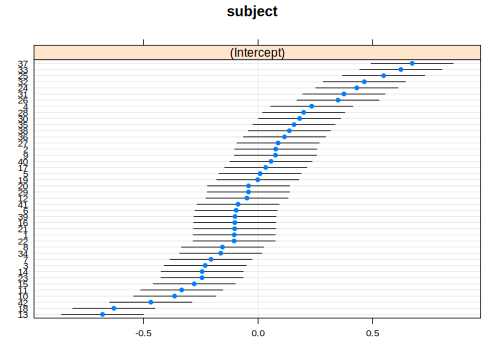
\includegraphics{Freq_CogSci_files/figure-latex/unnamed-chunk-109-1.pdf}

\hypertarget{the-formal-statement-of-the-varying-intercepts-model}{%
\subsection{The formal statement of the varying intercepts model}\label{the-formal-statement-of-the-varying-intercepts-model}}

The model \texttt{m0.lmer} above prints out the following type of linear model. \(i\) indexes subject, and \(j\) indexes items.

Once we know the subject id and the item id, we know which subject saw which condition:

\begin{Shaded}
\begin{Highlighting}[]
\KeywordTok{subset}\NormalTok{(gg05e1,subject}\OperatorTok{==}\DecValTok{1} \OperatorTok{&}\StringTok{ }\NormalTok{item }\OperatorTok{==}\StringTok{ }\DecValTok{1}\NormalTok{)}
\end{Highlighting}
\end{Shaded}

\begin{verbatim}
##   subject item condition rawRT so logrt
## 6       1    1    objgap   320  1 5.768
\end{verbatim}

The mathematical form of the linear mixed model is:

\begin{equation}
y_{ij} = \beta_0 + u_{0i}+\beta_1\times so_{ij} + \varepsilon_{ij}
\end{equation}

The \emph{only} new thing here beyond the linear model we saw earlier is the by-subject adjustment to the intercept. These by-subject adjustments to the intercept \(u_{0i}\) are assumed by lmer to come from a normal distribution centered around 0:

\begin{equation}
u_{0i} \sim Normal(0,\sigma_{u0})
\end{equation}

The ordinary linear model m0 has one intercept \(\beta_0\) for all subjects, whereas this linear mixed model with varying intercepts \texttt{m0.lmer} has a different intercept (\(\beta_0 + u_{0i}\)) for each subject \(i\).

We can visualize the adjustments for each subject to the intercepts as shown below.

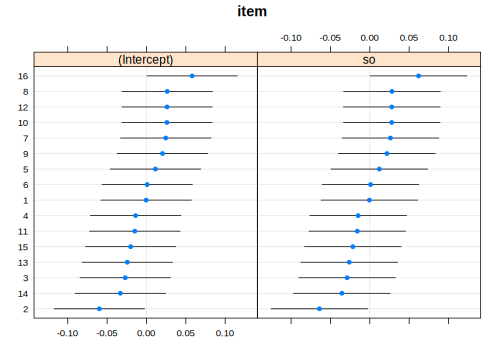
\includegraphics{Freq_CogSci_files/figure-latex/unnamed-chunk-111-1.pdf}

An important point is that in this model there are two variance components or sources of variance (cf.~the linear model, which had only one):

\begin{itemize}
\tightlist
\item
  \(u_0 \sim Normal(0,\sigma_{u0})\)
\item
  \(\varepsilon \sim Normal(0,\sigma)\)
\end{itemize}

These two standard deviations determine the standard error of the \(\beta_1\) slope parameter.

\hypertarget{model-type-2-varying-intercepts-and-slopes-without-a-correlation}{%
\subsection{Model type 2: Varying intercepts and slopes, without a correlation}\label{model-type-2-varying-intercepts-and-slopes-without-a-correlation}}

Unlike the figure associated with the \texttt{lmlist.fm1} model above, which also involves fitting separate models for each subject, the model \texttt{m0.lmer} assumes \emph{different intercepts} for each subject \emph{but the same slope}.

We can choose to fit different intercepts as well as different slopes for each subject. To achieve this, assume now that each subject's slope is also adjusted:

\begin{equation}
y_{ij} = \beta_0 + u_{0i}+(\beta_1+u_{1i})\times so_{ij} + \varepsilon_{ij}
\end{equation}

That is, we additionally assume that \(u_{1i} \sim Normal(0,\sigma_{u1})\). The \texttt{lmer} notation for fitting separate intercepts and slopes is \texttt{(1+so\textbar{}\textbar{}subject)}. We will just explain what the double vertical bars represent.

\begin{Shaded}
\begin{Highlighting}[]
\NormalTok{m1.lmer<-}\KeywordTok{lmer}\NormalTok{(logrt}\OperatorTok{~}\NormalTok{so}\OperatorTok{+}\NormalTok{(}\DecValTok{1}\OperatorTok{+}\NormalTok{so}\OperatorTok{||}\NormalTok{subject),gg05e1)}
\end{Highlighting}
\end{Shaded}

The output of this model will now show that there are not two but three sources of variability. These are:

\begin{itemize}
\tightlist
\item
  \(u_0 \sim Normal(0,\sigma_{u0})\)
\item
  \(u_1 \sim Normal(0,\sigma_{u1})\)
\item
  \(\varepsilon \sim Normal(0,\sigma)\)
\end{itemize}

In particular, the model estimates the following standard deviations:

\begin{itemize}
\tightlist
\item
  \(\hat\sigma_{u0}=0.317\)
\item
  \(\hat\sigma_{u1}=0.110\)
\item
  \(\hat\sigma = 0.365\).
\end{itemize}

\begin{verbatim}
Random effects:
 Groups    Name        Variance Std.Dev.
 subject   (Intercept) 0.1006   0.317   
 subject.1 so          0.0121   0.110   
 Residual              0.1336   0.365   
Number of obs: 672, groups:  subject, 42

Fixed effects:
            Estimate Std. Error t value
(Intercept)   5.8831     0.0509  115.50
so            0.0620     0.0221    2.81
\end{verbatim}

These fits for each subject are visualized below (the gray line shows the model with a single intercept and slope, i.e., our old model \texttt{m0}):

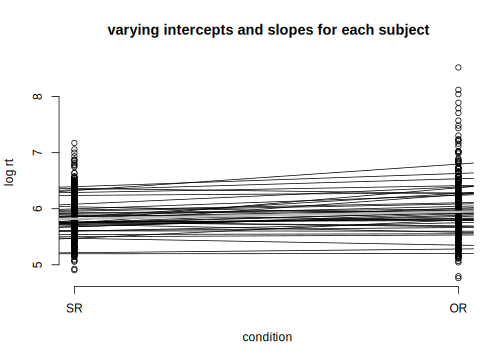
\includegraphics{Freq_CogSci_files/figure-latex/unnamed-chunk-113-1.pdf}

\hypertarget{comparing-lmlist-model-with-the-varying-intercepts-model}{%
\subsubsection{Comparing lmList model with the varying intercepts model}\label{comparing-lmlist-model-with-the-varying-intercepts-model}}

Compare this model with the \texttt{lmlist.fm1} model we fitted earlier:

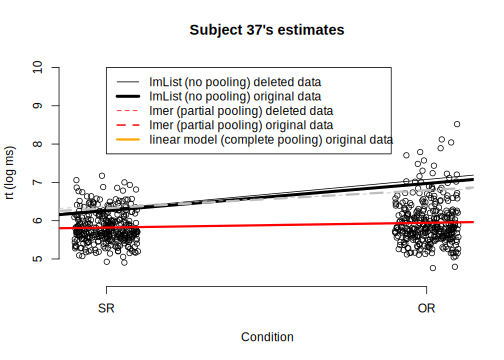
\includegraphics{Freq_CogSci_files/figure-latex/unnamed-chunk-114-1.pdf}

What is striking is that each subject's estimated best fit line is ``smoothed out'' compared to the lmList fits. This aspect of the linear mixed model is called shrinkage; we return to this point shortly.

\hypertarget{visualizing-random-effects}{%
\subsubsection{Visualizing random effects}\label{visualizing-random-effects}}

As before, it is instructive to visualize the by-subjects adjustments to the intercept and slope:

\begin{Shaded}
\begin{Highlighting}[]
\KeywordTok{print}\NormalTok{(}\KeywordTok{dotplot}\NormalTok{(}\KeywordTok{ranef}\NormalTok{(m1.lmer,}\DataTypeTok{condVar=}\OtherTok{TRUE}\NormalTok{)))}
\end{Highlighting}
\end{Shaded}

\begin{verbatim}
## $subject
\end{verbatim}

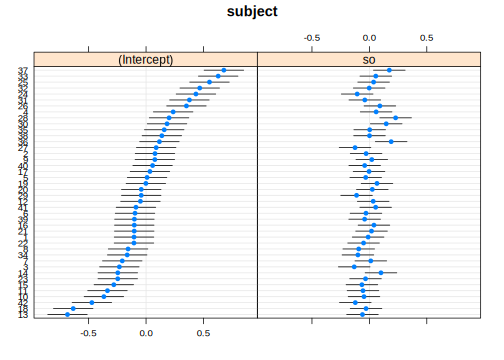
\includegraphics{Freq_CogSci_files/figure-latex/unnamed-chunk-115-1.pdf}

What this is showing is wide variability in the mean reading times between subjects, but very little variation in the slope between subjects.

\hypertarget{the-formal-statement-of-varying-intercepts-and-varying-slopes-linear-mixed-model}{%
\subsubsection{The formal statement of varying intercepts and varying slopes linear mixed model}\label{the-formal-statement-of-varying-intercepts-and-varying-slopes-linear-mixed-model}}

Here is the full statement of the varying intercept and slopes model. Again, i indexes subjects, j items.

\begin{equation}
y_{ij} = \beta_0 + u_{0i}+(\beta_1+u_{1i})\times so_{ij} + \varepsilon_{ij}
\end{equation}

There are now three variance components:

\begin{itemize}
\tightlist
\item
  \(u_0 \sim Normal(0,\sigma_{u0})\)
\item
  \(u_1 \sim Normal(0,\sigma_{u1})\)
\item
  \(\varepsilon \sim Normal(0,\sigma)\)
\end{itemize}

\hypertarget{crossed-random-effects-for-subjects-and-for-items}{%
\subsubsection{Crossed random effects for subjects and for items}\label{crossed-random-effects-for-subjects-and-for-items}}

The varying intercepts and slopes model doesn't capture all the sources of variance yet. The items also contribute sources of variance: just like subjects, items may also vary in their reading times or in the extent to which the reading times are impacted by condition. I other words, they might have different intercepts and slopes.

Notice that in this design (as in many designs in psycholinguistics or linguistic research) each subject sees all the items. In such cases, we say that subjects and items are crossed.

\begin{Shaded}
\begin{Highlighting}[]
\KeywordTok{head}\NormalTok{(}\KeywordTok{xtabs}\NormalTok{(}\OperatorTok{~}\NormalTok{subject}\OperatorTok{+}\NormalTok{item,gg05e1))}
\end{Highlighting}
\end{Shaded}

\begin{verbatim}
##        item
## subject 1 2 3 4 5 6 7 8 9 10 11 12 13 14 15 16
##       1 1 1 1 1 1 1 1 1 1  1  1  1  1  1  1  1
##       2 1 1 1 1 1 1 1 1 1  1  1  1  1  1  1  1
##       3 1 1 1 1 1 1 1 1 1  1  1  1  1  1  1  1
##       4 1 1 1 1 1 1 1 1 1  1  1  1  1  1  1  1
##       5 1 1 1 1 1 1 1 1 1  1  1  1  1  1  1  1
##       6 1 1 1 1 1 1 1 1 1  1  1  1  1  1  1  1
\end{verbatim}

Linear mixed model with crossed subject and items random effects can be defined with the following syntax:

\begin{Shaded}
\begin{Highlighting}[]
\NormalTok{m2.lmer<-}\KeywordTok{lmer}\NormalTok{(logrt}\OperatorTok{~}\NormalTok{so}\OperatorTok{+}\NormalTok{(}\DecValTok{1}\OperatorTok{+}\NormalTok{so}\OperatorTok{||}\NormalTok{subject)}\OperatorTok{+}
\NormalTok{(}\DecValTok{1}\OperatorTok{+}\NormalTok{so}\OperatorTok{||}\NormalTok{item),gg05e1)}
\end{Highlighting}
\end{Shaded}

Analogously to the preceding example, now there are five variance components:

\begin{verbatim}
Random effects:
 Groups    Name        Variance Std.Dev.
 subject   (Intercept) 0.10090  0.3177  
 subject.1 so          0.01224  0.1106  
 item      (Intercept) 0.00127  0.0356  
 item.1    so          0.00162  0.0402  
 Residual              0.13063  0.3614  
Number of obs: 672, groups:  subject, 42; item, 16

Fixed effects:
            Estimate Std. Error t value
(Intercept)   5.8831     0.0517  113.72
so            0.0620     0.0242    2.56
\end{verbatim}

The item intercept and slope adjustments can be visualized as well. Notice that there is a lot less item-level variation; this is often the case in planned experiments in sentence processing, where the experimental items are carefully constructed to vary as little as possible.

\begin{Shaded}
\begin{Highlighting}[]
\KeywordTok{print}\NormalTok{(}\KeywordTok{dotplot}\NormalTok{(}\KeywordTok{ranef}\NormalTok{(m2.lmer,}\DataTypeTok{condVar=}\OtherTok{TRUE}\NormalTok{))}\OperatorTok{$}\NormalTok{item)}
\end{Highlighting}
\end{Shaded}

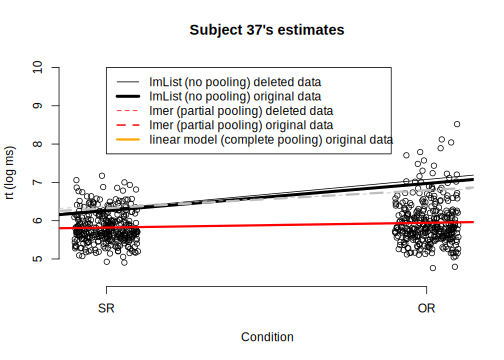
\includegraphics{Freq_CogSci_files/figure-latex/unnamed-chunk-118-1.pdf}

In the above models, there is an assumption that there is no correlation between the intercept and slope adjustments by subject, and no correlation between the intercept and slope adjustments by item. It is possible that the intercept and slope adjustments are in fact correlated. We turn to this model next.

\hypertarget{model-type-3-varying-intercepts-and-varying-slopes-with-correlation}{%
\subsection{Model type 3: Varying intercepts and varying slopes, with correlation}\label{model-type-3-varying-intercepts-and-varying-slopes-with-correlation}}

A correlation can be introduced between the intercept and slope adjustments by using a single vertical bar instead of two vertical bars in the random effects structure:

\begin{Shaded}
\begin{Highlighting}[]
\NormalTok{m3.lmer<-}\KeywordTok{lmer}\NormalTok{(logrt}\OperatorTok{~}\NormalTok{so}\OperatorTok{+}\NormalTok{(}\DecValTok{1}\OperatorTok{+}\NormalTok{so}\OperatorTok{|}\NormalTok{subject)}\OperatorTok{+}\NormalTok{(}\DecValTok{1}\OperatorTok{+}\NormalTok{so}\OperatorTok{|}\NormalTok{item),}
\NormalTok{              gg05e1)}
\end{Highlighting}
\end{Shaded}

\begin{verbatim}
## boundary (singular) fit: see ?isSingular
\end{verbatim}

To understand what this model is doing, we have to recall what a bivariate/multivariate distribution is.

\begin{verbatim}
Random effects:
 Groups   Name        Variance Std.Dev. Corr
 subject  (Intercept) 0.10103  0.3178       
          so          0.01228  0.1108   0.58
 item     (Intercept) 0.00172  0.0415       
          so          0.00196  0.0443   1.00 <= degeneracy
 Residual             0.12984  0.3603       
Number of obs: 672, groups:  subject, 42; item, 16

Fixed effects:
            Estimate Std. Error t value
(Intercept)   5.8831     0.0520  113.09
so            0.0620     0.0247    2.51
\end{verbatim}

The correlations (0.58 and 1.00) you see in the model output below are the correlations between the varying intercepts and slopes for subjects and for items. Notice that the variance covariance matrix for items is degenerate: its correlation is 1. This matrix cannot be inverted.

When the correlation is +1 or -1 or near these numbers, this means that the optimizer in lme4 is unable to estimate the correlation parameter, usually due to there not being enough data. If you are in such a situation, you are better off not trying to estimate this parameter with the data you have, and instead fitting one of the simpler models. We will return to this point when discussing model selection. For further discussion, see \citet{barr2013}, \citet{BatesEtAlParsimonious}, and \citet{hannesBEAP}.

\hypertarget{formal-statement-of-varying-intercepts-and-varying-slopes-linear-mixed-model-with-correlation}{%
\subsubsection{Formal statement of varying intercepts and varying slopes linear mixed model with correlation}\label{formal-statement-of-varying-intercepts-and-varying-slopes-linear-mixed-model-with-correlation}}

As usual, i indexes subjects, j items. The vector \texttt{so} is the sum-coded factor levels: +1 for object relatives and -1 for subject relatives. The only new thing in this model is the item-level effects, and the specification of the variance-covariance matrix for subjects and items, in order to include the correlation parameters.

\begin{equation}
y_{ij} = \alpha + u_{0i} + w_{0j} + (\beta + u_{1i} + w_{1j}) \times so_{ij} + \varepsilon_{ij}
\end{equation}

where \(\varepsilon_{ij} \sim Normal(0,\sigma)\) and

\begin{equation}\label{eq:covmatLM}
\Sigma_u
=
\begin{pmatrix}
\sigma _{u0}^2  & \rho _{u}\sigma _{u0}\sigma _{u1}\\
\rho _{u}\sigma _{u0}\sigma _{u1}    & \sigma _{u1}^2\\
\end{pmatrix}
\quad 
\Sigma _w
=
\begin{pmatrix}
\sigma _{w0}^2  & \rho _{w}\sigma _{w0}\sigma _{w1}\\
\rho _{w}\sigma _{w0}\sigma _{w1}    & \sigma _{w1}^2\\
\end{pmatrix}
\end{equation}

\begin{equation}\label{eq:jointpriordistLM}
\begin{pmatrix}
  u_0 \\ 
  u_1 \\
\end{pmatrix}
\sim 
\mathcal{N} \left(
\begin{pmatrix}
  0 \\
  0 \\
\end{pmatrix},
\Sigma_{u}
\right),
\quad
\begin{pmatrix}
  w_0 \\ 
  w_1 \\
\end{pmatrix}
\sim 
\mathcal{N}\left(
\begin{pmatrix}
  0 \\
  0 \\
\end{pmatrix},
\Sigma_{w}
\right)
\end{equation}

\hypertarget{visualizing-the-random-effects}{%
\subsubsection{Visualizing the random effects}\label{visualizing-the-random-effects}}

One can visualize the correlation between intercepts and slopes by subjects. The positive correlation of 0.58 between subject intercept and slope adjustments implies that slower subjects show larger effects. However, the dotplot below doesn't show a convincing indication that such a correlation exists:

\begin{Shaded}
\begin{Highlighting}[]
\KeywordTok{print}\NormalTok{(}\KeywordTok{dotplot}\NormalTok{(}\KeywordTok{ranef}\NormalTok{(m3.lmer,}\DataTypeTok{condVar=}\OtherTok{TRUE}\NormalTok{))}\OperatorTok{$}\NormalTok{subject)}
\end{Highlighting}
\end{Shaded}

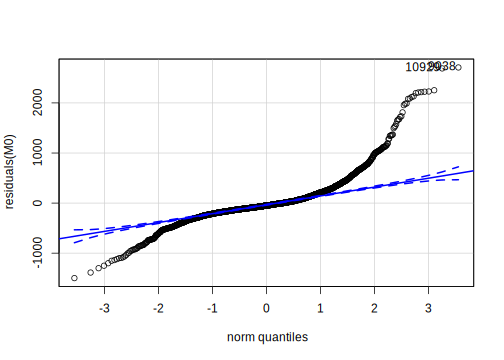
\includegraphics{Freq_CogSci_files/figure-latex/unnamed-chunk-120-1.pdf}

The correlation pattern is easier to see if we plot the slope adjustments against the intercept adjustments.

\begin{Shaded}
\begin{Highlighting}[]
\KeywordTok{plot}\NormalTok{(}\KeywordTok{ranef}\NormalTok{(m3.lmer)}\OperatorTok{$}\NormalTok{subject[,}\DecValTok{1}\NormalTok{],}\KeywordTok{ranef}\NormalTok{(m3.lmer)}\OperatorTok{$}\NormalTok{subject[,}\DecValTok{2}\NormalTok{],}
\DataTypeTok{xlab=}\StringTok{"Intercept adjustments (subject)"}\NormalTok{,}
\DataTypeTok{ylab=}\StringTok{"Slope adjustments"}\NormalTok{)}
\end{Highlighting}
\end{Shaded}

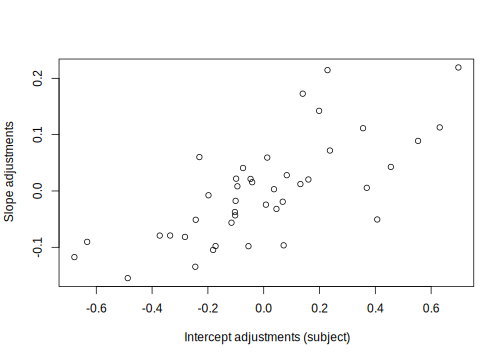
\includegraphics{Freq_CogSci_files/figure-latex/unnamed-chunk-121-1.pdf}

When we talk about hypothesis testing, we will look at what inferences we can draw from this correlation.

The dotplot showing the item-level effects shows a perfect correlation between intercept and slope adjustments, but as mentioned above these are from a degenerate variance covariance matrix and not meaningful.

\begin{Shaded}
\begin{Highlighting}[]
\KeywordTok{print}\NormalTok{(}\KeywordTok{dotplot}\NormalTok{(}\KeywordTok{ranef}\NormalTok{(m3.lmer,}\DataTypeTok{condVar=}\OtherTok{TRUE}\NormalTok{))}\OperatorTok{$}\NormalTok{item)}
\end{Highlighting}
\end{Shaded}

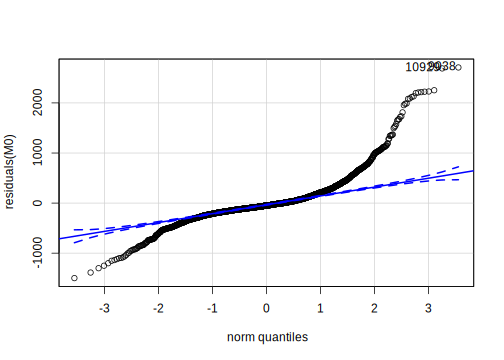
\includegraphics{Freq_CogSci_files/figure-latex/unnamed-chunk-122-1.pdf}

\hypertarget{shrinkage-in-linear-mixed-models}{%
\section{Shrinkage in linear mixed models}\label{shrinkage-in-linear-mixed-models}}

The estimate of the effect for each participant computed from a linear mixed model is ``pushed'' towards the grand mean effect compared to when we fit a separate linear model to each subject's data.
This is called ``shrinkage'' in linear mixed models. We say that the individual-level estimates are shrunk towards the mean slope.
The less data we have from a given subject, the greater the shrinkage.

\begin{figure}
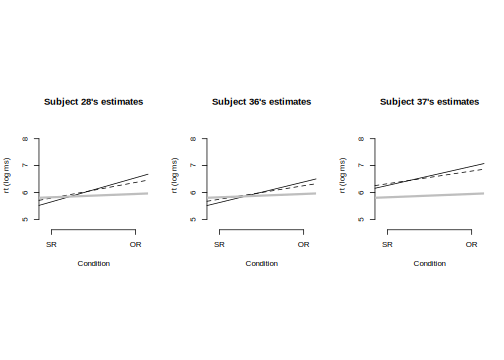
\includegraphics[width=0.75\linewidth]{Freq_CogSci_files/figure-latex/shrinkage-1} \caption{The figures show linear model fits (the grand mean estimates) for three subjects; shown are the simple linear model fit on all the data (gray line), the lmList model fit to the individual subject's data (black line), and the linear mixed model fit (the broken line). In all three subjects' models, the linear mixed model estimates are shrunk towards the grand mean (gray line) estimates.}\label{fig:shrinkage}
\end{figure}

\hypertarget{shrinkage-in-action-when-data-are-missing}{%
\subsubsection{Shrinkage in action: when data are missing}\label{shrinkage-in-action-when-data-are-missing}}

The importance and value of shrinkage becomes clear once we simulate a situation where there is some missing data. Missingness can happen in experiments, either due to lost measurements (arising from computer error or programming errors), or some other reason. To see what happens when we have missing data, let's randomly delete some data from one subject. We will randomly delete 50\% of subject 37's data:

\begin{Shaded}
\begin{Highlighting}[]
\KeywordTok{set.seed}\NormalTok{(}\DecValTok{4321}\NormalTok{)}
\CommentTok{## choose some data randomly to remove:}
\NormalTok{rand<-}\KeywordTok{rbinom}\NormalTok{(}\DecValTok{1}\NormalTok{,}\DataTypeTok{n=}\DecValTok{16}\NormalTok{,}\DataTypeTok{prob=}\FloatTok{0.5}\NormalTok{)}
\end{Highlighting}
\end{Shaded}

Here are subject 37's reading times (16 data points):

\begin{Shaded}
\begin{Highlighting}[]
\NormalTok{gg05e1[}\KeywordTok{which}\NormalTok{(gg05e1}\OperatorTok{$}\NormalTok{subject}\OperatorTok{==}\DecValTok{37}\NormalTok{),]}\OperatorTok{$}\NormalTok{rawRT}
\end{Highlighting}
\end{Shaded}

\begin{verbatim}
##  [1]  770  536  686  578  457  487 2419  884 3365  233
## [11]  715  671 1104  281 1081  971
\end{verbatim}

Now, we randomly delete half the data:

\begin{Shaded}
\begin{Highlighting}[]
\NormalTok{gg05e1}\OperatorTok{$}\NormalTok{deletedRT<-gg05e1}\OperatorTok{$}\NormalTok{rawRT}
\NormalTok{gg05e1[}\KeywordTok{which}\NormalTok{(gg05e1}\OperatorTok{$}\NormalTok{subject}\OperatorTok{==}\DecValTok{37}\NormalTok{),]}\OperatorTok{$}\NormalTok{deletedRT<-}
\StringTok{  }
\StringTok{  }\KeywordTok{ifelse}\NormalTok{(rand,}\OtherTok{NA}\NormalTok{,}
\NormalTok{         gg05e1[}\KeywordTok{which}\NormalTok{(gg05e1}\OperatorTok{$}\NormalTok{subject}\OperatorTok{==}\DecValTok{37}\NormalTok{),]}\OperatorTok{$}\NormalTok{rawRT)}
\end{Highlighting}
\end{Shaded}

Now subject 37's estimates are going to be pretty wild, because they are based on much less data (even one extreme value can strongly influence the mean):

\begin{Shaded}
\begin{Highlighting}[]
\KeywordTok{subset}\NormalTok{(gg05e1,subject}\OperatorTok{==}\DecValTok{37}\NormalTok{)}\OperatorTok{$}\NormalTok{deletedRT}
\end{Highlighting}
\end{Shaded}

\begin{verbatim}
##  [1]  770   NA  686  578   NA   NA   NA   NA 3365  233
## [11]   NA  671 1104   NA   NA  971
\end{verbatim}

\begin{verbatim}
## [1] 6.617
\end{verbatim}

\begin{verbatim}
## [1] 0.3554
\end{verbatim}

\begin{verbatim}
## [1] 6.688
\end{verbatim}

\begin{verbatim}
## [1] 0.3884
\end{verbatim}

Now fit the hierarchical model and examine subject 37's estimates on undeleted vs deleted data:

\begin{figure}
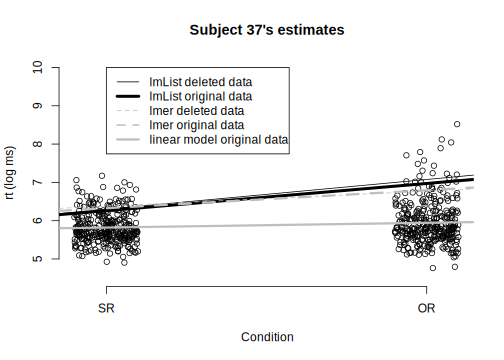
\includegraphics[width=0.75\linewidth]{Freq_CogSci_files/figure-latex/shrinkage2-1} \caption{The figure shows linear model fits (the grand mean estimates) for subject 37. When using lmList, deleting data leads to very different estimates; but using lmer, deleting half the data from this subject hardly affects the individual subject's estimates.}\label{fig:shrinkage2}
\end{figure}

What we see here is that the estimates from the hierarchical model are barely affected by the missingness, but the estimates from the lmList model are heavily affected.
This means that linear mixed models will give you more robust estimates (think Type M error!) compared to models which fit data sepaarately for each subject. This property of shrinkage is one reason why linear mixed models are so important in cognitive science.

\hypertarget{summary}{%
\section{Summary}\label{summary}}

\hypertarget{sec:LMExercises1}{%
\section{Exercises}\label{sec:LMExercises1}}

Download the data-set E1\_data.csv. Then run the following commands to load the \texttt{lme4} library and to set up your data for analysis:

\begin{Shaded}
\begin{Highlighting}[]
\KeywordTok{library}\NormalTok{(lme4)}

\CommentTok{## load data:}
\NormalTok{dat<-}\KeywordTok{read.csv}\NormalTok{(}\StringTok{"data/E1_data.csv"}\NormalTok{,}\DataTypeTok{header=}\OtherTok{TRUE}\NormalTok{)}
\CommentTok{## convert RT to milliseconds:}
\NormalTok{dat}\OperatorTok{$}\NormalTok{RT<-dat}\OperatorTok{$}\NormalTok{RT}\OperatorTok{*}\DecValTok{1000}
\CommentTok{## choose critical region:}
\NormalTok{word_n<-}\DecValTok{4}
\CommentTok{## subset critical data:}
\NormalTok{crit<-}\KeywordTok{subset}\NormalTok{(dat,Position}\OperatorTok{==}\NormalTok{word_n)}
\end{Highlighting}
\end{Shaded}

The data consist of a repeated measures experiment comparing two conditions which are labeled Type 1 and Type 2. The column Sub refers to subject id, and the column ID refers to item id. RT refers to reading time in seconds (we have converted it above to milliseconds); NA is missing data. You can ignore the other columns. This is a standard Latin square design. We will work with the data frame \texttt{crit} below.

\hypertarget{sec:LMExercisesPart1}{%
\subsection{By-subjects t-test}\label{sec:LMExercisesPart1}}

Using RT as a dependent variable, carry out the appropriate by-subjects t-test to evaluate the null hypothesis that there is no difference between the conditions labeled Type 1 and 2. Write down all the R commands needed to do the appropriate t-test, and the resulting t-value and p-value. State whether we can reject the null hypothesis given the results of the t-test; explain why.

\hypertarget{sec:LMExercisesPart2}{%
\subsection{Fitting a linear mixed model}\label{sec:LMExercisesPart2}}

Now, using the data-frame called \texttt{crit} above, fit a linear mixed model (called M0). Recode the column called Type as sum contrasts.

Assume varying intercepts for subjects and varying intercepts for items (varying intercepts are sometimes called random intercepts). Write down the linear mixed models command, and write down the fixed-effects estimates (intercept and slope) along with their standard errors. State whether we can reject the null hypothesis given the results of the t-value shown in the linear mixed model output; explain why.

\hypertarget{sec:LMExercisesPart3}{%
\subsection{t-test vs.~linear mixed model}\label{sec:LMExercisesPart3}}

Why do the results of the t-test and the linear mixed model M0 differ?

\hypertarget{sec:LMExercisesPart4}{%
\subsection{Power calculation using power.t.test}\label{sec:LMExercisesPart4}}

The researcher wants to achieve 80\% statistical power in a future study. Based on the available data above, she determines that the standard error (note: not the standard deviation!) of the difference in means between the conditions Type 1 and Type 2 is 21. She has reason to believe that the true difference in means is 30 ms. What is the number of participants (to the nearest whole number) needed to achieve approximately 80\% power? Use the power.t.test function to compute your answer. Write down the \texttt{power.t.test} function specification you used, as well as the number of participants needed, based on the output of the power.t.test function.

\hypertarget{sec:LMExercisesPart5}{%
\subsection{Residuals}\label{sec:LMExercisesPart5}}

The plot below shows the distribution of the residuals from model M0 plotted against the standard normal distribution with mean 0 and standard deviation 1. Explain what the plot tells us about one of the model assumptions of the linear mixed model M0 that you fit earlier.

(You can ignore the numbers below the plot.)

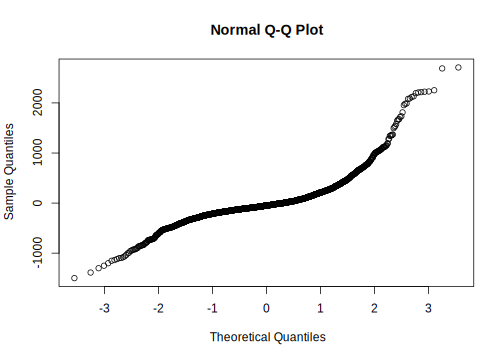
\includegraphics{Freq_CogSci_files/figure-latex/unnamed-chunk-134-1.pdf}

\hypertarget{sec:LMExercisesPart6}{%
\subsection{Understanding contrast coding}\label{sec:LMExercisesPart6}}

Using only your estimates of the intercept and the slope in model M0's fixed effects output, write down the mean of the condition labeled Type 1 in the data, and the mean of the condition labeled Type 2.

\hypertarget{sec:LMExercisesPart7}{%
\subsection{Understanding the fixed-effects output}\label{sec:LMExercisesPart7}}

Suppose that the model M0's output for the fixed effects analysis were as follows. SO is a sum-coded contrast specification for the conditions in the column labeled Type.

\begin{Shaded}
\begin{Highlighting}[]
\NormalTok{results}
\end{Highlighting}
\end{Shaded}

\begin{verbatim}
##             Estimate Std. Error t value
## (Intercept)   686.01      47.54   14.43
## SO             18.94         NA    2.00
\end{verbatim}

What is the value of the standard error of the slope (SO), which is labeled NA above?

\hypertarget{sec:LMExercisesPart8}{%
\subsection{Understanding the null hypothesis test}\label{sec:LMExercisesPart8}}

A researcher fits a linear mixed model to compare the reading times between two conditions (a) and (b), just like in the above study. Her hypothesis is that the mean for condition (a) is larger than the mean for (b). She observes that condition a has sample mean 500 ms, and condition (b) has sample mean 450 ms. She also establishes from the linear mixed model that the t-value is 1.94. The approximate p-value associated with this t-value is 0.052. Answer the following: (A) Do we have evidence against the null hypothesis and (B) do we have evidence for the particular research hypothesis that the researcher has?

The researcher runs the same analysis as above on a new data-set that has the same design as above, and now gets a p-value of 0.001. Now she has stronger evidence than in the above case where the p-value was 0.052. What does she have stronger evidence for?

\hypertarget{hypothesis-testing-using-the-likelihood-ratio-test}{%
\chapter{Hypothesis testing using the likelihood ratio test}\label{hypothesis-testing-using-the-likelihood-ratio-test}}

We started the book with the one-sample t-test. There, we had the following procedure:

\begin{itemize}
\tightlist
\item
  Given independent and identically distributed data \(y\), define a null hypothesis: \(H_0: \mu=\mu_0\)
\item
  Compute the sample mean \(\bar{y}\) and the standard error SE
\item
  Reject the null hypothesis if the absolute value of \(\bar{y}/SE\) is larger than \(2\).
\end{itemize}

Here, we turn to a closely related test: the \emph{likelihood ratio test statistic}.

\hypertarget{the-likelihood-ratio-test-the-theory}{%
\section{The likelihood ratio test: The theory}\label{the-likelihood-ratio-test-the-theory}}

Suppose that \(X_1,\dots, X_n\) are independent and normally distributed with mean \(\mu\) and standard deviation \(\sigma\) (assume for simplicity that \(\sigma\) is known).

Let the null hypothesis be \(H_0: \mu=\mu_0\) and the alternative be \(H_1: \mu\neq \mu_0\). Here, \(\mu_0\) is a number, such as \(0\).

The likelihood of the data \(y\) can be computed under the null model, in which \(\mu=\mu_0\), and under the alternative model, in which \(\mu\) has some specific alternative value. To make this concrete, imagine 10 data points being generated from a Normal(0,1).

\begin{Shaded}
\begin{Highlighting}[]
\NormalTok{y<-}\KeywordTok{rnorm}\NormalTok{(}\DecValTok{10}\NormalTok{)}
\end{Highlighting}
\end{Shaded}

We can compute the joint likelihood under a null hypothesis that \(\mu=0\):

\begin{Shaded}
\begin{Highlighting}[]
\NormalTok{likNULL<-}\KeywordTok{prod}\NormalTok{(}\KeywordTok{dnorm}\NormalTok{(y,}\DataTypeTok{mean=}\DecValTok{0}\NormalTok{,}\DataTypeTok{sd=}\DecValTok{1}\NormalTok{))}
\NormalTok{likNULL}
\end{Highlighting}
\end{Shaded}

\begin{verbatim}
## [1] 9.151e-06
\end{verbatim}

On the log scale, we would need to add the log likelihoods of each data point:

\begin{Shaded}
\begin{Highlighting}[]
\NormalTok{loglikNULL<-}\KeywordTok{sum}\NormalTok{(}\KeywordTok{dnorm}\NormalTok{(y,}\DataTypeTok{mean=}\DecValTok{0}\NormalTok{,}\DataTypeTok{sd=}\DecValTok{1}\NormalTok{,}\DataTypeTok{log=}\OtherTok{TRUE}\NormalTok{))}
\NormalTok{loglikNULL}
\end{Highlighting}
\end{Shaded}

\begin{verbatim}
## [1] -11.6
\end{verbatim}

Similarly, we can compute the log likelihood with \(\mu\) equal to the maximum likelihood estimate of \(\mu\), the sample mean.

\begin{Shaded}
\begin{Highlighting}[]
\NormalTok{loglikALT<-}\KeywordTok{sum}\NormalTok{(}\KeywordTok{dnorm}\NormalTok{(y,}\DataTypeTok{mean=}\KeywordTok{mean}\NormalTok{(y),}\DataTypeTok{sd=}\DecValTok{1}\NormalTok{,}\DataTypeTok{log=}\OtherTok{TRUE}\NormalTok{))}
\NormalTok{loglikALT}
\end{Highlighting}
\end{Shaded}

\begin{verbatim}
## [1] -11.59
\end{verbatim}

Essentially, the likelihood ratio test compares the ratio of likelihoods of the two models; on the log scale, the difference in log likelihood is taken. This is because a ratio on the log scale becomes a difference. The likelihood ratio test then chooses the model with the higher log likelihood, provided that the higher likelihood is high enough (we will just make this more precise).

One can specify the test in general terms as follows. Suppose that the likelihood is with respect to some parameter \(\theta\). We can evaluate the likelihood at \(\mu_0\), the null hypothesis value of the parameter, and evaluate the likelihood using the maximum likelihood estimate \(\hat\theta\) of the parameter, as we did above. The likelihood ratio can then be written as follows:

\begin{equation}
\Lambda = \frac{max_{\theta\in \omega_0}(lik(\theta))}{max_{\theta\in \omega_1)}(lik(\theta))}
\end{equation}

where, \(\omega_0=\{\mu_0\}\) and \(\omega_1=\{\forall \mu \mid \mu\neq \mu_0\}\). The function max just selects the maximum value of any choices of parameter values; in the case of the null hypothesis there is only one value, \(\mu_0\). In the case of the alternative model, the maximum likelihood estimate \(\hat\theta\) is the maximum value.

Now, assuming that the data are coming from a normal distribution, the numerator of the likelihood ratio statistic is:

\begin{equation}
lik(\theta=\mu_0) = \frac{1}{(\sigma\sqrt{2\pi})^n} 
           exp\left( -\frac{1}{2\sigma^2} \sum_{i=1}^n (X_i - \mu_0)^2  \right)
\end{equation}

For the denominator, the MLE \(\bar{X}\) is taken as \(\mu\):

\begin{equation}
lik(\theta=\bar{X}) =\frac{1}{(\sigma\sqrt{2\pi})^n} exp \left( -\frac{1}{2\sigma^2} \sum_{i=1}^n (X_i - \bar{X})^2 \right)
\end{equation}

The likelihood ratio statistic is then:

\begin{equation}
\Lambda = \frac{lik(\theta=\mu_0)}{lik(\theta=\bar{X})}=
\frac{\frac{1}{(\sigma\sqrt{2\pi})^n} 
           exp\left( -\frac{1}{2\sigma^2} \sum_{i=1}^n (X_i - \mu_0)^2  \right)}{\frac{1}{(\sigma\sqrt{2\pi})^n} 
           exp\left( -\frac{1}{2\sigma^2} \sum_{i=1}^n (X_i - \bar{X})^2  \right)}
\end{equation}

Canceling out common terms:

\begin{equation}
\Lambda = 
\frac{exp\left( -\frac{1}{2\sigma^2} \sum_{i=1}^n (X_i - \mu_0)^2  \right)}{
        exp\left( -\frac{1}{2\sigma^2} \sum_{i=1}^n (X_i - \bar{X})^2  \right)}
\end{equation}

Taking logs:

\begin{equation}
\begin{split}
\log \Lambda =& 
\left( -\frac{1}{2\sigma^2} \sum_{i=1}^n (X_i - \mu_0)^2  \right)-\left( -\frac{1}{2\sigma^2} \sum_{i=1}^n (X_i - \bar{X})^2  \right)\\
=& -\frac{1}{2\sigma^2} \left( \sum_{i=1}^n (X_i - \mu_0)^2  -  \sum_{i=1}^n (X_i - \bar{X})^2 \right)\\
\end{split}
\end{equation}

Now, it is a standard algebraic trick to rewrite \(\sum_{i=1}^n (X_i -\mu_0)^2\) as a sum of two terms:

\begin{equation}
\sum_{i=1}^n (X_i -\mu_0)^2 = \sum_{i=1}^n (X_i - \bar{X})^2 + n(\bar{X} - \mu_0)^2 
\end{equation}

If we rearrange terms, we obtain:

\begin{equation}
\sum_{i=1}^n (X_i -\mu_0)^2 - \sum_{i=1}^n (X_i - \bar{X})^2 = n(\bar{X} - \mu_0)^2 
\end{equation}

Now, we just established above that \(\log \Lambda\) is:

\begin{equation}
\log \Lambda= -\frac{1}{2\sigma^2} \left( \sum_{i=1}^n (X_i - \mu_0)^2  -  \sum_{i=1}^n (X_i - \bar{X})^2 \right)
\end{equation}

Consider the term in the brackets:

\begin{equation}
(\sum_{i=1}^n (X_i - \mu_0)^2  -  \sum_{i=1}^n (X_i - \bar{X})^2)
\end{equation}

This can be rewritten as:

\begin{equation}
n(\bar{X} - \mu_0)^2
\end{equation}

Rewriting in this way gives us:

\begin{equation}
\log \Lambda = -\frac{1}{2\sigma^2}   n(\bar{X} - \mu_0)^2 
\end{equation}

Rearranging terms:

\begin{equation}
-2 \log \Lambda =    \frac{n(\bar{X} - \mu_0)^2 }{\sigma^2}
\end{equation}

Or even more transparently:

\begin{equation}
-2 \log \Lambda =    \frac{(\bar{X} - \mu_0)^2 }{\frac{\sigma^2}{n}}
\end{equation}

This should remind you of the t-test! Basically, just like in the t-test, what this is saying is that we reject the null when \(\mid \bar{X} - \mu_0\mid\), or negative two times the difference in log likelihood, is large!

Now we will define what it means for \(-2\log \Lambda\) to be large. There is a theorem in statistics that states that for large \(n\), the distribution of \(-2\log \Lambda\) approaches the chi-squared distribution, with degrees of freedom corresponding to the difference in the number of parameters between the two models being compared.

We will define the \emph{likelihood ratio test statistic}, call it \(LRT\), as follows. Here, \(Lik(\theta)\) refers to the likelihood given some value \(\theta\) for the parameter, and
\(logLik(\theta)\) refers to the log likelihood.

\begin{equation}
\begin{split}
LRT =& -2\times (Lik(\theta_0)/Lik(\theta_1)) \\
\log LRT =& -2\times \{logLik(\theta_0)-logLik(\theta_1)\}\\
\end{split}
\end{equation}

where \(\theta_1\) and \(\theta_0\) are the estimates of \(\theta\) under the alternative and null hypotheses, respectively. The likelihood ratio test rejects \(H_0\) if \(\log LRT\) is sufficiently large. As the sample size approaches infinity, \(\log LRT\) approaches the chi-squared distribution:

\begin{equation}
\log LRT \rightarrow \chi_r^2  \hbox{ as }  n \rightarrow \infty
\end{equation}

Here, \(r\) is called the degrees of freedom and is the difference in the number of parameters under the null and alternative hypotheses.

The above result is called \emph{Wilks' theorem}. The proof of Wilks' theorem is fairly involved but you can find it in Lehmann's textbook \emph{Testing Statistical Hypotheses}.

Note that sometimes you will see the form:

\begin{equation}
 \log LRT = 2 \{logLik(\theta_1) - logLik(\theta_0)\}
\end{equation}

It should be clear that both statements are saying the same thing; in the second case, we are just subtracting the null hypothesis log likelihood from the alternative hypothesis log likelihood, so the negative sign disappears.

That's the theory. Let's see how the likelihood ratio test works for (a) simulated data, and (b) our running example, the English relative clause data from \citet{grodner}.

\hypertarget{a-practical-example-using-simulated-data}{%
\section{A practical example using simulated data}\label{a-practical-example-using-simulated-data}}

A practical example will make the usage of this test clear.
Let's just simulate data from a linear model:

\begin{Shaded}
\begin{Highlighting}[]
\NormalTok{x<-}\DecValTok{1}\OperatorTok{:}\DecValTok{10}
\NormalTok{y<-}\StringTok{ }\DecValTok{10} \OperatorTok{+}\StringTok{ }\DecValTok{20}\OperatorTok{*}\NormalTok{x}\OperatorTok{+}\KeywordTok{rnorm}\NormalTok{(}\DecValTok{10}\NormalTok{,}\DataTypeTok{sd=}\DecValTok{10}\NormalTok{)}
\end{Highlighting}
\end{Shaded}

Here, the null hypothesis that the slope is 0 is false (it has value 20). Now, we fit a null hypothesis model, without a slope:

\begin{Shaded}
\begin{Highlighting}[]
\CommentTok{## null hypothesis model:}
\NormalTok{m0<-}\KeywordTok{lm}\NormalTok{(y}\OperatorTok{~}\DecValTok{1}\NormalTok{)}
\end{Highlighting}
\end{Shaded}

We will compare this model's log likelihood with that of the alternative model, which includes an estimate of the slope:

\begin{Shaded}
\begin{Highlighting}[]
\CommentTok{## alternative hypothesis model:}
\NormalTok{m1<-}\KeywordTok{lm}\NormalTok{(y}\OperatorTok{~}\NormalTok{x)}
\end{Highlighting}
\end{Shaded}

The difference in log likelihood, multiplied with -2, is:

\begin{Shaded}
\begin{Highlighting}[]
\NormalTok{LogLRT<-}\StringTok{ }\DecValTok{-2}\OperatorTok{*}\NormalTok{(}\KeywordTok{logLik}\NormalTok{(m0)}\OperatorTok{-}\KeywordTok{logLik}\NormalTok{(m1))}
\CommentTok{## observed value:}
\NormalTok{LogLRT[}\DecValTok{1}\NormalTok{]}
\end{Highlighting}
\end{Shaded}

\begin{verbatim}
## [1] 34.49
\end{verbatim}

The difference in the number of parameters in the two models is one, so \(\log LRT\) has the distribution \(\chi_1^2\). Is the observed value \(34.49\) unexpected under this distribution? We can calculate the probability of obtaining the likelihood ratio statistic we observed above, or a value more extreme, given the \(\chi_1^2\) distribution.

\begin{Shaded}
\begin{Highlighting}[]
\KeywordTok{pchisq}\NormalTok{(LogLRT[}\DecValTok{1}\NormalTok{],}\DataTypeTok{df=}\DecValTok{1}\NormalTok{,}\DataTypeTok{lower.tail=}\OtherTok{FALSE}\NormalTok{)}
\end{Highlighting}
\end{Shaded}

\begin{verbatim}
## [1] 4.286e-09
\end{verbatim}

Just like the critical t-value in the t-test, the critical chi-squared value here is:

\begin{Shaded}
\begin{Highlighting}[]
\CommentTok{## critical value:}
\KeywordTok{qchisq}\NormalTok{(}\FloatTok{0.95}\NormalTok{,}\DataTypeTok{df=}\DecValTok{1}\NormalTok{)}
\end{Highlighting}
\end{Shaded}

\begin{verbatim}
## [1] 3.841
\end{verbatim}

If minus two times the observed difference in log likelihood is larger than this critical value, we reject the null hypothesis.

Note that in the likelihood test above, we are comparing one nested model against another: the null hypothesis model is nested inside the alternative hypothesis model. What this means is that the alternative hypothesis model contains all the parameters in the null hypothesis model (i.e., the intercept) plus another one (the slope).

\hypertarget{a-real-life-example-the-english-relative-clause-data}{%
\section{A real-life example: The English relative clause data}\label{a-real-life-example-the-english-relative-clause-data}}

The likelihood ratio test is also the way that hypothesis testing is done with the linear mixed model. Here is how it works. Let's look again at the \citet{grodner} English relative clause data. The null hypothesis here refers to the slope parameter. When we have the sum contrast coding, the intercept \(\beta_0\) refers to the grand mean, and the slope \(\beta_1\) is the amount by which subject and object relative clause mean reading times deviate from the grand mean. Testing the null hypothesis that \(\beta_1\) is 0 amounts to testing whether there is any difference in means between the two relative clause types. This becomes clear if we consider the following.

Let object relatives be coded as \(+1\) and subject relatives as \(-1\). Then, the mean reading time \(\mu_{or}\) for object relatives in the linear mixed model is:

\begin{equation}
\mu_{or}=\beta_0 + \beta_1
\end{equation}

Similarly, the mean reading time \(\mu_{sr}\) for subject relatives is:

\begin{equation}
\mu_{sr}=\beta_0 - \beta_1
\end{equation}

If the null hypothesis is that \(\mu_{or}-\mu_{sr}=0\), then this amounts to saying that:

\begin{equation}
(\beta_0 + \beta_1)-(\beta_0 - \beta_1)=0
\end{equation}

Removing the brackets gives us:

\begin{equation}
\beta_0 + \beta_1-\beta_0 + \beta_1 = 0
\end{equation}

This yields the equation:

\begin{equation} \label{eq:nullhypsumcontrast}
2\beta_1= 0
\end{equation}

Dividing both sides of the equation by 2, we get the null hypothesis that \(\beta_1=0\).

Incidentally, if we had rescaled the contrast coding to be not \(\pm 1\) but \(\pm 1/2\), the parameter \(\beta_1\) would represent exactly the difference between the two means, and null hypothesis in equation \eqref{eq:nullhypsumcontrast} would have come out to be \(\beta_1= 0\). This is why it is sometimes better to recode the contrasts as \(\pm 1/2\) rather than \(\pm 1\). See \citet{SchadEtAlcontrasts} for details; we will discuss this in the contrast coding chapter as well.

Let's load the data, set up the contrast coding, and fit the null versus the alternative models. We will fit varying intercept and varying slopes for subject and item, without correlations for items. We don't attempt to fit a model with by-items varying intercepts and slopes with a correlation because we would get a singularity in the variance covariance matrix.

\begin{Shaded}
\begin{Highlighting}[]
\NormalTok{gg05e1<-}\KeywordTok{read.table}\NormalTok{(}\StringTok{"data/grodnergibsonE1crit.txt"}\NormalTok{,}\DataTypeTok{header=}\OtherTok{TRUE}\NormalTok{)}

\NormalTok{gg05e1}\OperatorTok{$}\NormalTok{so <-}\StringTok{ }\KeywordTok{ifelse}\NormalTok{(gg05e1}\OperatorTok{$}\NormalTok{condition}\OperatorTok{==}\StringTok{"objgap"}\NormalTok{,}\DecValTok{1}\NormalTok{,}\OperatorTok{-}\DecValTok{1}\NormalTok{)}
\NormalTok{gg05e1}\OperatorTok{$}\NormalTok{logrt<-}\KeywordTok{log}\NormalTok{(gg05e1}\OperatorTok{$}\NormalTok{rawRT)}

\KeywordTok{library}\NormalTok{(lme4)}
\NormalTok{m0<-}\KeywordTok{lmer}\NormalTok{(logrt}\OperatorTok{~}\DecValTok{1} \OperatorTok{+}\StringTok{ }\NormalTok{(}\DecValTok{1}\OperatorTok{+}\NormalTok{so}\OperatorTok{|}\NormalTok{subject)}\OperatorTok{+}\NormalTok{(}\DecValTok{1}\OperatorTok{+}\NormalTok{so}\OperatorTok{||}\NormalTok{item),gg05e1)}
\NormalTok{m1<-}\KeywordTok{lmer}\NormalTok{(logrt}\OperatorTok{~}\DecValTok{1} \OperatorTok{+}\StringTok{ }\NormalTok{so }\OperatorTok{+}\StringTok{ }\NormalTok{(}\DecValTok{1}\OperatorTok{+}\NormalTok{so}\OperatorTok{|}\NormalTok{subject)}\OperatorTok{+}\NormalTok{(}\DecValTok{1}\OperatorTok{+}\NormalTok{so}\OperatorTok{||}\NormalTok{item),gg05e1)}
\end{Highlighting}
\end{Shaded}

Notice that we keep all random effects in the null model. We say that the null model is nested inside the full model.

Next, we compare the two models' log likelihoods. There is a function in the \texttt{lme4} package that achieves that: the \texttt{anova} function:

\begin{Shaded}
\begin{Highlighting}[]
\KeywordTok{anova}\NormalTok{(m0,m1)}
\end{Highlighting}
\end{Shaded}

\begin{verbatim}
## refitting model(s) with ML (instead of REML)
\end{verbatim}

\begin{verbatim}
## Data: gg05e1
## Models:
## m0: logrt ~ 1 + (1 + so | subject) + ((1 | item) + (0 + so | item))
## m1: logrt ~ 1 + so + (1 + so | subject) + ((1 | item) + (0 + so | 
## m1:     item))
##    npar AIC BIC logLik deviance Chisq Df Pr(>Chisq)
## m0    7 707 739   -347      693                    
## m1    8 703 739   -343      687  6.15  1      0.013
\end{verbatim}

You can confirm from the output that the \texttt{Chisq} value shown is minus two times the difference in log likelihood of the two models. The p-value is computed using the chi-squared distribution with one degree of freedom because in the two models the difference in the number of parameters is one:

\begin{Shaded}
\begin{Highlighting}[]
\KeywordTok{round}\NormalTok{(}\KeywordTok{pchisq}\NormalTok{(}\FloatTok{6.15}\NormalTok{,}\DataTypeTok{df=}\DecValTok{1}\NormalTok{,}\DataTypeTok{lower.tail=}\OtherTok{FALSE}\NormalTok{),}\DecValTok{3}\NormalTok{)}
\end{Highlighting}
\end{Shaded}

\begin{verbatim}
## [1] 0.013
\end{verbatim}

It is common in the psycholinguistics literature to use the t-value from the linear mixed model output to conduct the hypothesis test on the slope:

\begin{Shaded}
\begin{Highlighting}[]
\KeywordTok{summary}\NormalTok{(m1)}\OperatorTok{$}\NormalTok{coefficients}
\end{Highlighting}
\end{Shaded}

\begin{verbatim}
##             Estimate Std. Error t value
## (Intercept)  5.88306    0.05176 113.669
## so           0.06202    0.02422   2.561
\end{verbatim}

The most general method for hypothesis testing is the likelihood ratio test shown above. One can use the t-test output from the linear mixed model for hypothesis testing, but this should be done only when the data are balanced. If there is lack of balance (e.g., missing data for whatever reason), the likelihood ratio test is the best way to proceed. In any case, when we talk about the evidence against the null hypothesis, the likelihood ratio test is the only reasonable way to talk about what evidence we have. See \citet{Royall} for more discussion of this point. The essence of Royall's point is that the most reasonable way to talk about the evidence in favor of a particular model is with reference to, i.e., relative to, a baseline model.

One can also use the likelihood ratio test to evaluate whether a variance component should be included or not. For example, is the correlation parameter justified for the subjects random effects? Recall that we had a correlation of 0.58. Is this statistically significant? One can test this in the following way:

\begin{Shaded}
\begin{Highlighting}[]
\NormalTok{m1<-}\KeywordTok{lmer}\NormalTok{(logrt}\OperatorTok{~}\DecValTok{1} \OperatorTok{+}\StringTok{ }\NormalTok{so }\OperatorTok{+}\StringTok{ }\NormalTok{(}\DecValTok{1}\OperatorTok{+}\NormalTok{so}\OperatorTok{|}\NormalTok{subject)}\OperatorTok{+}\NormalTok{(}\DecValTok{1}\OperatorTok{+}\NormalTok{so}\OperatorTok{||}\NormalTok{item),gg05e1)}
\NormalTok{m1NoCorr<-}\KeywordTok{lmer}\NormalTok{(logrt}\OperatorTok{~}\DecValTok{1} \OperatorTok{+}\StringTok{ }\NormalTok{so }\OperatorTok{+}\StringTok{ }\NormalTok{(}\DecValTok{1}\OperatorTok{+}\NormalTok{so}\OperatorTok{||}\NormalTok{subject)}\OperatorTok{+}\NormalTok{(}\DecValTok{1}\OperatorTok{+}\NormalTok{so}\OperatorTok{||}\NormalTok{item),gg05e1)}
\KeywordTok{anova}\NormalTok{(m1,m1NoCorr)}
\end{Highlighting}
\end{Shaded}

\begin{verbatim}
## refitting model(s) with ML (instead of REML)
\end{verbatim}

\begin{verbatim}
## Data: gg05e1
## Models:
## m1NoCorr: logrt ~ 1 + so + ((1 | subject) + (0 + so | subject)) + ((1 | 
## m1NoCorr:     item) + (0 + so | item))
## m1: logrt ~ 1 + so + (1 + so | subject) + ((1 | item) + (0 + so | 
## m1:     item))
##          npar AIC BIC logLik deviance Chisq Df
## m1NoCorr    7 710 741   -348      696         
## m1          8 703 739   -343      687   8.7  1
##          Pr(>Chisq)
## m1NoCorr           
## m1           0.0032
\end{verbatim}

The test indicates that we can reject the null hypothesis that the correlation parameter is 0. We will return to this parameter in the chapter on simulation.

A final point: the likelihood ratio has essentially the same logic as the t-test, and that includes the fact that the focus is on the rejection of the null. The null cannot be accepted in the face of a null result, unless there is a good case to be made that power is sufficiently high (we will investigate this point later, in the simulation chapter). Also, since the likelihood ratio depends on defining the alternative model using the maximum likelihood estimate (the sample mean), it suffers from exactly the same problem as the t-test (Type M errors in the face of low power). We will also investigate this point in the simulation chapter.

\hypertarget{sec:HypTestExercises}{%
\section{Exercises}\label{sec:HypTestExercises}}

\hypertarget{sec:HypTestExercisesChinese}{%
\subsection{Chinese relative clauses}\label{sec:HypTestExercisesChinese}}

Load the following two data-sets:

\begin{Shaded}
\begin{Highlighting}[]
\NormalTok{gibsonwu<-}\KeywordTok{read.table}\NormalTok{(}\StringTok{"data/gibsonwucrit.txt"}\NormalTok{,}
                     \DataTypeTok{header=}\OtherTok{TRUE}\NormalTok{)}
\NormalTok{gibsonwu2<-}\KeywordTok{read.table}\NormalTok{(}\StringTok{"data/gibsonwu2012datarepeat.txt"}\NormalTok{,}
                      \DataTypeTok{header=}\OtherTok{TRUE}\NormalTok{)}
\end{Highlighting}
\end{Shaded}

The data are taken from two experiments that investigate (inter alia) the effect of relative clause type on reading time in Chinese. The data are from \citet{gibsonwu} and \citet{VasishthetalPLoSOne2013} respectively. The second data-set is a direct replication attempt of the first.

Chinese relative clauses are interesting theoretically because they are prenominal: the relative clause appears before the head noun.

As iscussed in \citet{gibsonwu}, the consequence of Chinese relative clauses being prenominal is that the distance between the gap in relative clause and the head noun is larger in subject relatives than object relatives. \citet{hsiao03} were the first to suggest that the larger distance in subject relatives leads to longer reading time at the head noun. Under this view, the prediction is that subject relatives are harder to process than object relatives. If this is true, this is interesting because in most other languages that have been studied, subject relatives are easier to process than object relatives; so Chinese will be a very unusual exception cross-linguistically.

The data provided are for the critical region (the head noun). The experiment method is self-paced reading, so we have reading times in milliseconds.

The research hypothesis is whether the difference in reading times between object and subject relative clauses is negative. For both data-sets, investigate this question by (a) fitting a paired t-test (by-subjects and by items), (b) fitting the most complex linear mixed model you can to the data and then interpreting the t-value, and (c) the likelihood ratio test. What can we conclude about the research question?

\hypertarget{sec:HypTestExerciseAgrmt}{%
\subsection{Agreement attraction in comprehension}\label{sec:HypTestExerciseAgrmt}}

Load the following data:

\begin{Shaded}
\begin{Highlighting}[]
\NormalTok{datE1<-}\KeywordTok{read.table}\NormalTok{(}\StringTok{"data/dillonE1.txt"}\NormalTok{,}\DataTypeTok{header=}\OtherTok{TRUE}\NormalTok{)}
\end{Highlighting}
\end{Shaded}

The data are taken from an experiment that investigate (inter alia) the effect of number similarity between a noun and the auxiliary verb in sentences like the following. There are two levels to a factor called Int(erference): low and high.

\begin{enumerate}
\def\labelenumi{(\alph{enumi})}
\tightlist
\item
  low: The key to the cabinet \emph{are} on the table
\item
  high: The key to the \emph{cabinets} \emph{are} on the table
\end{enumerate}

Here, in (b), the auxiliary verb \emph{are} is predicted to be read faster than in (a), because the plural marking on the noun \emph{cabinets} leads the reader to think that the sentence is grammatical. (Note that both sentences are ungrammatical.) This phenomenon, where the high condition is read faster than the low condition, is called \textbf{agreement attraction}.

The data provided are for the critical region (the auxiliary verb \emph{are}). The experiment method is eyetracking; we have total reading times in milliseconds.

The research question is whether the difference in reading times between high and low conditions is negative.

\begin{itemize}
\tightlist
\item
  First, figure out which linear mixed model is appropriate for these data (varying intercepts only? varying intercepts and slopes? with or without correlations?).
\item
  Then, carry out a statistical test using (a) the paired t-test (using the t.test function), (b) the t-test of the linear mixed model, and (c) the likelihood ratio test. What is your conclusion? Is there evidence for agreement attraction in the data?
\end{itemize}

\hypertarget{sec:HypTestExerciseGramCE}{%
\subsection{The grammaticality illusion}\label{sec:HypTestExerciseGramCE}}

Load the following data-sets:

\begin{Shaded}
\begin{Highlighting}[]
\NormalTok{english<-}\KeywordTok{read.table}\NormalTok{(}\StringTok{"data/embeddingenglish.txt"}\NormalTok{,}
                    \DataTypeTok{header=}\OtherTok{TRUE}\NormalTok{)}
\NormalTok{dutch<-}\KeywordTok{read.table}\NormalTok{(}\StringTok{"data/embeddingdutch.txt"}\NormalTok{,}
                  \DataTypeTok{header=}\OtherTok{TRUE}\NormalTok{)}
\end{Highlighting}
\end{Shaded}

In an offline accuracy rating study on English double center-embedding constructions, \citet{gibsonthomas99} found that grammatical constructions (e.g., example a below) were no less acceptable than ungrammatical constructions (e.g., example b) where a middle verb phrase (e.g., was cleaning every week) was missing.

\begin{enumerate}
\def\labelenumi{(\alph{enumi})}
\item
  The apartment that the maid who the service had sent over was cleaning every week was well decorated.
\item
  *The apartment that the maid who the service had sent over --- was well decorated
\end{enumerate}

Based on these results from English, \citet{gibsonthomas99} proposed that working-memory overload leads the comprehender to forget the prediction of the upcoming verb phrase (VP), which reduces working-memory load. This came to be known as the \emph{VP-forgetting hypothesis}. The prediction is that in the word immediately following the final verb, the grammatical condition (which is coded as +1 in the data-frames) should be harder to read than the ungrammatical condition (which is coded as -1).

The data provided above test this hypothesis using self-paced reading for English \citep{VSLK08}, and for Dutch \citep{FrankEtAl2015}. The data provided are for the critical region (the noun phrase, labeled NP1, following the final verb). We have reading times in log milliseconds.

Is there support for the VP-forgetting hypothesis cross-linguistically, from English and Dutch?

\hypertarget{ch:LMtheory}{%
\chapter{Linear modeling theory}\label{ch:LMtheory}}

So far, we have been studying linear models and linear mixed models rather informally. This approach is good enough for a first-pass at linear modeling. However, in order to fully understand the underlying machinery of linear models, the matrix formulation of the linear model is extremely important and useful. There is a price to be paid, however: one has to reactivate one's knowledge of matrix algebra, or one has to put in some work into reviewing elementary matrix theory. Fortunately, reviewing these concepts is not too difficult. We begin this chapter with a quick review of some basic concepts in matrix algebra, and then apply them to linear modeling. One very useful set of online lectures on the basic ideas behind linear algebra is the short set of videos by 3Blue1Brown: \url{https://youtu.be/kjBOesZCoqc}. You should look at these videos before reading the next section, if you have never encountered the basic concepts behind matrix algebra.

\hypertarget{a-quick-review-of-some-basic-concepts-in-matrix-algebra}{%
\section{A quick review of some basic concepts in matrix algebra}\label{a-quick-review-of-some-basic-concepts-in-matrix-algebra}}

A rectangular array of numbers (real numbers in our case), with \(n\) rows and \(m\) columns, is a matrix. The main application for us will be in solving systems of linear equations in statistics.

An example of a \(2\times 2\) matrix:

\begin{Shaded}
\begin{Highlighting}[]
\CommentTok{## a 2x2 matrix:}
\NormalTok{(m1<-}\KeywordTok{matrix}\NormalTok{(}\DecValTok{1}\OperatorTok{:}\DecValTok{4}\NormalTok{,}\DecValTok{2}\NormalTok{,}\DecValTok{2}\NormalTok{))}
\end{Highlighting}
\end{Shaded}

\begin{verbatim}
##      [,1] [,2]
## [1,]    1    3
## [2,]    2    4
\end{verbatim}

An important operation on matrices is the transpose: the rows become columns and the columns rows. If \(X\) is matrix, \(X^T\) is its transpose. R has a function \texttt{t()} that transposes a matrix:

\begin{Shaded}
\begin{Highlighting}[]
\CommentTok{## transpose of a matrix:}
\KeywordTok{t}\NormalTok{(m1)}
\end{Highlighting}
\end{Shaded}

\begin{verbatim}
##      [,1] [,2]
## [1,]    1    2
## [2,]    3    4
\end{verbatim}

\hypertarget{matrix-addition-subtraction-and-multiplication}{%
\subsection{Matrix addition, subtraction, and multiplication}\label{matrix-addition-subtraction-and-multiplication}}

Matrix addition and subtraction are easy, they are cell-wise operations. An example shows how this works:

\begin{Shaded}
\begin{Highlighting}[]
\NormalTok{m1}\OperatorTok{+}\NormalTok{m1}
\end{Highlighting}
\end{Shaded}

\begin{verbatim}
##      [,1] [,2]
## [1,]    2    6
## [2,]    4    8
\end{verbatim}

\begin{Shaded}
\begin{Highlighting}[]
\NormalTok{m1}\OperatorTok{-}\NormalTok{m1}
\end{Highlighting}
\end{Shaded}

\begin{verbatim}
##      [,1] [,2]
## [1,]    0    0
## [2,]    0    0
\end{verbatim}

Matrix multiplication is defined as follows. Think of this simple situation first, where you have a vector of values:

\begin{Shaded}
\begin{Highlighting}[]
\NormalTok{(m2<-}\KeywordTok{rnorm}\NormalTok{(}\DecValTok{5}\NormalTok{))}
\end{Highlighting}
\end{Shaded}

\begin{verbatim}
## [1] -0.17650 -0.99922 -1.24649 -0.75233 -0.07495
\end{verbatim}

\begin{Shaded}
\begin{Highlighting}[]
\CommentTok{## this is a vector:}
\KeywordTok{str}\NormalTok{(m2)}
\end{Highlighting}
\end{Shaded}

\begin{verbatim}
##  num [1:5] -0.177 -0.999 -1.246 -0.752 -0.075
\end{verbatim}

If you want to find out the sum of the squares of these values (\(\overset{n}{\underset{i=1}\sum} x_i ^2\)), then you can multiply each value \(x_i\) in m2 with itself, and sum up the result. This is called a \textbf{dot product} of two vectors (here, \(m2\) repeated twice):

\(x_1 \cdot x_1+x_2 \cdot x_2+x_3 \cdot x_3+x_4 \cdot x_4+x_5 \cdot x_5\)

Using R:

\begin{Shaded}
\begin{Highlighting}[]
\NormalTok{(}\KeywordTok{sum}\NormalTok{(m2}\OperatorTok{*}\NormalTok{m2))}
\end{Highlighting}
\end{Shaded}

\begin{verbatim}
## [1] 3.155
\end{verbatim}

An important observation we will need later is that if two vectors are orthogonal, i.e., at 90 degrees to one another, then their dot product is 0. A simple example is two vectors on the cartesian plane that go along the x and y axes:

\begin{Shaded}
\begin{Highlighting}[]
\NormalTok{v1<-}\KeywordTok{c}\NormalTok{(}\DecValTok{0}\NormalTok{,}\DecValTok{1}\NormalTok{)}
\NormalTok{v2<-}\KeywordTok{c}\NormalTok{(}\DecValTok{1}\NormalTok{,}\DecValTok{0}\NormalTok{)}
\KeywordTok{sum}\NormalTok{(v1}\OperatorTok{*}\NormalTok{v2)}
\end{Highlighting}
\end{Shaded}

\begin{verbatim}
## [1] 0
\end{verbatim}

Matrix multiplication does exactly the above dot product operation (for arbitrarily large matrices). In R, matrix multiplication is carried out using a special operator (the * operator we are used to using for multiplication is used only for ordinary scalar multiplication). Notice that we have first converted the vector with \(5\) cells into a \(5\times 1\) matrix:

\begin{Shaded}
\begin{Highlighting}[]
\KeywordTok{t}\NormalTok{(}\KeywordTok{matrix}\NormalTok{(m2))}
\end{Highlighting}
\end{Shaded}

\begin{verbatim}
##         [,1]    [,2]   [,3]    [,4]     [,5]
## [1,] -0.1765 -0.9992 -1.246 -0.7523 -0.07495
\end{verbatim}

\begin{Shaded}
\begin{Highlighting}[]
\KeywordTok{matrix}\NormalTok{(m2)}
\end{Highlighting}
\end{Shaded}

\begin{verbatim}
##          [,1]
## [1,] -0.17650
## [2,] -0.99922
## [3,] -1.24649
## [4,] -0.75233
## [5,] -0.07495
\end{verbatim}

\begin{Shaded}
\begin{Highlighting}[]
\KeywordTok{t}\NormalTok{(}\KeywordTok{matrix}\NormalTok{(m2))}\OperatorTok\KeywordTok{matrix}\NormalTok{(m2)}
\end{Highlighting}
\end{Shaded}

\begin{verbatim}
##       [,1]
## [1,] 3.155
\end{verbatim}

Note that two matrices can only be multiplied if they are \textbf{conformable}: the number of columns of the first matrix has to be the same as the number of rows of the second matrix. So, if you have an \(1\times 5\) matrix, you can multiply it with an \(5\times 1\) matrix, and the end result of the multiplication will be an \(1\times 1\) matrix (i.e., a scalar value). In the above example, the vector m2, converted to a matrix, is \(5\times 1\) in dimensions; you cannot multiply a \(5\times 1\) with a \(5\times 1\) matrix, but the transform of m2 to a \(1\times 5\) matrix can be multiplied with the \(5\times 1\) matrix.

More generally, if you have an \(n\times m\) matrix and multiply it with an \(m\times p\) matrix, you will get a \(n\times p\) matrix, and the operations we have to do is the dot product operation, repeatedly applied to each row of the first matrix and each column of the second matrix. For example:

\begin{Shaded}
\begin{Highlighting}[]
\NormalTok{X1<-}\KeywordTok{matrix}\NormalTok{(}\KeywordTok{rnorm}\NormalTok{(}\DecValTok{4}\NormalTok{),}\DataTypeTok{ncol=}\DecValTok{2}\NormalTok{)}
\NormalTok{X2<-}\KeywordTok{matrix}\NormalTok{(}\KeywordTok{rnorm}\NormalTok{(}\DecValTok{4}\NormalTok{),}\DataTypeTok{ncol=}\DecValTok{2}\NormalTok{)}
\CommentTok{## matrix multiplication:}
\NormalTok{X1}\OperatorTok\NormalTok{X2}
\end{Highlighting}
\end{Shaded}

\begin{verbatim}
##       [,1]   [,2]
## [1,] 1.680 -1.677
## [2,] 2.655 -2.610
\end{verbatim}

\begin{Shaded}
\begin{Highlighting}[]
\CommentTok{## is a series of dot products of vectors:}
\KeywordTok{sum}\NormalTok{(X1[}\DecValTok{1}\NormalTok{,] }\OperatorTok{*}\StringTok{ }\NormalTok{X2[,}\DecValTok{1}\NormalTok{])}
\end{Highlighting}
\end{Shaded}

\begin{verbatim}
## [1] 1.68
\end{verbatim}

\begin{Shaded}
\begin{Highlighting}[]
\KeywordTok{sum}\NormalTok{(X1[}\DecValTok{1}\NormalTok{,] }\OperatorTok{*}\StringTok{ }\NormalTok{X2[,}\DecValTok{2}\NormalTok{])}
\end{Highlighting}
\end{Shaded}

\begin{verbatim}
## [1] -1.677
\end{verbatim}

\begin{Shaded}
\begin{Highlighting}[]
\KeywordTok{sum}\NormalTok{(X1[}\DecValTok{2}\NormalTok{,] }\OperatorTok{*}\StringTok{ }\NormalTok{X2[,}\DecValTok{1}\NormalTok{])}
\end{Highlighting}
\end{Shaded}

\begin{verbatim}
## [1] 2.655
\end{verbatim}

\begin{Shaded}
\begin{Highlighting}[]
\KeywordTok{sum}\NormalTok{(X1[}\DecValTok{2}\NormalTok{,] }\OperatorTok{*}\StringTok{ }\NormalTok{X2[,}\DecValTok{2}\NormalTok{])}
\end{Highlighting}
\end{Shaded}

\begin{verbatim}
## [1] -2.61
\end{verbatim}

Scalar matrix multiplication is easy. Multiplying a matrix M with a scalar value just amounts to multiplying the scalar with each cell of the matrix. The order of multiplication doesn't matter:

\begin{Shaded}
\begin{Highlighting}[]
\DecValTok{5}\OperatorTok{*}\NormalTok{m2}
\end{Highlighting}
\end{Shaded}

\begin{verbatim}
## [1] -0.8825 -4.9961 -6.2324 -3.7617 -0.3748
\end{verbatim}

\begin{Shaded}
\begin{Highlighting}[]
\NormalTok{m2}\OperatorTok{*}\DecValTok{5}
\end{Highlighting}
\end{Shaded}

\begin{verbatim}
## [1] -0.8825 -4.9961 -6.2324 -3.7617 -0.3748
\end{verbatim}

\hypertarget{diagonal-matrix-and-identity-matrix}{%
\subsection{Diagonal matrix and identity matrix}\label{diagonal-matrix-and-identity-matrix}}

A diagonal matrix is a square matrix that has zeros in its off-diagonals:

\begin{Shaded}
\begin{Highlighting}[]
\KeywordTok{diag}\NormalTok{(}\KeywordTok{c}\NormalTok{(}\DecValTok{1}\NormalTok{,}\DecValTok{2}\NormalTok{,}\DecValTok{4}\NormalTok{))}
\end{Highlighting}
\end{Shaded}

\begin{verbatim}
##      [,1] [,2] [,3]
## [1,]    1    0    0
## [2,]    0    2    0
## [3,]    0    0    4
\end{verbatim}

An identity matrix is a diagonal matrix with 1's along its diagonal:

\begin{Shaded}
\begin{Highlighting}[]
\KeywordTok{diag}\NormalTok{(}\KeywordTok{rep}\NormalTok{(}\DecValTok{1}\NormalTok{,}\DecValTok{3}\NormalTok{))}
\end{Highlighting}
\end{Shaded}

\begin{verbatim}
##      [,1] [,2] [,3]
## [1,]    1    0    0
## [2,]    0    1    0
## [3,]    0    0    1
\end{verbatim}

For a \(3\times 3\) identity matrix, we can write \(I_3\), and for an nxn identity matrix, \(I_n\).

Multiplying an identity matrix with any (conformable) matrix gives that matrix back:

\begin{Shaded}
\begin{Highlighting}[]
\NormalTok{(I<-}\KeywordTok{diag}\NormalTok{(}\KeywordTok{c}\NormalTok{(}\DecValTok{1}\NormalTok{,}\DecValTok{1}\NormalTok{)))}
\end{Highlighting}
\end{Shaded}

\begin{verbatim}
##      [,1] [,2]
## [1,]    1    0
## [2,]    0    1
\end{verbatim}

\begin{Shaded}
\begin{Highlighting}[]
\NormalTok{(m3<-}\KeywordTok{matrix}\NormalTok{(}\KeywordTok{c}\NormalTok{(}\DecValTok{6}\NormalTok{,}\DecValTok{7}\NormalTok{,}\DecValTok{8}\NormalTok{,}\DecValTok{9}\NormalTok{),}\DecValTok{2}\NormalTok{,}\DecValTok{2}\NormalTok{))}
\end{Highlighting}
\end{Shaded}

\begin{verbatim}
##      [,1] [,2]
## [1,]    6    8
## [2,]    7    9
\end{verbatim}

\begin{Shaded}
\begin{Highlighting}[]
\NormalTok{(I}\OperatorTok\NormalTok{m3)}
\end{Highlighting}
\end{Shaded}

\begin{verbatim}
##      [,1] [,2]
## [1,]    6    8
## [2,]    7    9
\end{verbatim}

\begin{Shaded}
\begin{Highlighting}[]
\CommentTok{## the matrix does not have to be square:}
\NormalTok{(m4<-}\KeywordTok{matrix}\NormalTok{(}\KeywordTok{c}\NormalTok{(}\DecValTok{2}\NormalTok{,}\DecValTok{3}\NormalTok{,}\DecValTok{6}\NormalTok{,}\DecValTok{7}\NormalTok{,}\DecValTok{8}\NormalTok{,}\DecValTok{9}\NormalTok{),}\DecValTok{2}\NormalTok{,}\DecValTok{3}\NormalTok{))}
\end{Highlighting}
\end{Shaded}

\begin{verbatim}
##      [,1] [,2] [,3]
## [1,]    2    6    8
## [2,]    3    7    9
\end{verbatim}

\begin{Shaded}
\begin{Highlighting}[]
\NormalTok{(I}\OperatorTok\NormalTok{m4)}
\end{Highlighting}
\end{Shaded}

\begin{verbatim}
##      [,1] [,2] [,3]
## [1,]    2    6    8
## [2,]    3    7    9
\end{verbatim}

\hypertarget{powers-of-matrices}{%
\subsection{Powers of matrices}\label{powers-of-matrices}}

If A is a square \(n\times n\) matrix, then we write \(AA\) as \(A^2\), and so on. If A is diagonal, then \(AA\) is just the diagonal matrix with the diagonal elements of A squared:

\begin{Shaded}
\begin{Highlighting}[]
\NormalTok{m<-}\KeywordTok{diag}\NormalTok{(}\KeywordTok{c}\NormalTok{(}\DecValTok{1}\NormalTok{,}\DecValTok{2}\NormalTok{,}\DecValTok{3}\NormalTok{))}
\NormalTok{m}\OperatorTok\NormalTok{m}
\end{Highlighting}
\end{Shaded}

\begin{verbatim}
##      [,1] [,2] [,3]
## [1,]    1    0    0
## [2,]    0    4    0
## [3,]    0    0    9
\end{verbatim}

For all positive integers \(m\), \(I_n^m = I_n\).

\hypertarget{inverse-of-a-matrix}{%
\subsection{Inverse of a matrix}\label{inverse-of-a-matrix}}

If \(A,B\) are square matrices, of order \(n\times n\), and the following relation is satisfied:

\begin{equation}
AB = BA= I_n
\end{equation}

then, \(B\) is the inverse (it is unique) of \(A\). We write \(B=A^{-1}\). The inverse is analogous to division and allows us to solve matrix equations: AB=C can be solved by post-multiplying both sides by \(B^{-1}\) to get \(ABB^{-1}=AI=A=CB^{-1}\).

Pre-multiplying a matrix like \(A\) above by its inverse \(A^{-1}\) gives an identity matrix (the R function \texttt{solve} computes the inverse of a matrix):

\begin{Shaded}
\begin{Highlighting}[]
\NormalTok{(m5<-}\KeywordTok{matrix}\NormalTok{(}\KeywordTok{c}\NormalTok{(}\DecValTok{2}\NormalTok{,}\DecValTok{3}\NormalTok{,}\DecValTok{4}\NormalTok{,}\DecValTok{5}\NormalTok{),}\DecValTok{2}\NormalTok{,}\DecValTok{2}\NormalTok{))}
\end{Highlighting}
\end{Shaded}

\begin{verbatim}
##      [,1] [,2]
## [1,]    2    4
## [2,]    3    5
\end{verbatim}

\begin{Shaded}
\begin{Highlighting}[]
\NormalTok{(}\KeywordTok{round}\NormalTok{(}\KeywordTok{solve}\NormalTok{(m5)}\OperatorTok\NormalTok{m5))}
\end{Highlighting}
\end{Shaded}

\begin{verbatim}
##      [,1] [,2]
## [1,]    1    0
## [2,]    0    1
\end{verbatim}

If a matrix is not invertible, we say that it is \textbf{singular}.

A useful fact to know about non-singular matrices is the following relationship. If A and B are non-singular matrices then \((AB)^{-1} = B^{-1}A^{-1}\).

\hypertarget{linear-independence-and-rank}{%
\subsection{Linear independence, and rank}\label{linear-independence-and-rank}}

An important concept in matrices is linear independence. Consider a \(3\times 3\) matrix.
The rows \(r_1, r_2, r_3\) are linearly \textbf{dependent} if
\(\alpha, \beta, \gamma\), not all zero, exist such that
\(\alpha r_1+ \beta r_2+ \gamma r_3 = (0,0,0)\).

If the rows or columns of a matrix A are linearly dependent, then the matrix is singular, i.e., it is not invertible.

Linear independence leads us to the concept of the rank of a matrix.
The column rank of a matrix is the maximum number of linearly independent columns in the matrix. The row rank is the maximum number of linearly independent rows. Column rank is always equal to row rank, so we can just call it rank.

The above is the minimum vocabulary we need to understand the linear model in its matrix form. Let us now turn to the matrix formulation of the linear model.

\hypertarget{the-essentials-of-linear-modeling-theory}{%
\section{The essentials of linear modeling theory}\label{the-essentials-of-linear-modeling-theory}}

Consider a deterministic function \(\phi(\mathbf{x},\beta)\) which takes as input some variable values \(x\) and some fixed values \(\beta\). A simple example would be some variable \(x\) determining the value of another variable \(y\) by multiplying \(x\) with \(\beta\).

\begin{equation}
y = \beta x
\end{equation}

Another example with two fixed values \(\beta_0\) and \(\beta_1\) determining \(y\) is:

\begin{equation}
y = \beta_0 + \beta_1 x
\end{equation}

We can rewrite the above equation in matrix form as follows.

\begin{equation}
\begin{split}
y=& \beta_0 + \beta_1 x\\
=& \beta_0\times 1 + \beta_1 x\\
=& \begin{pmatrix}
1 & x\\
\end{pmatrix}
\begin{pmatrix}
\beta_0 \\
\beta_1 \\
\end{pmatrix}
\end{split}
\end{equation}

Because \(y\) is a function of \(x\) and the \(2\times 1\) matrix \(\beta=[\beta_0 \beta_1]^T\), the most general way to write the above function is as we did above:

\begin{equation}
y = \phi(x,\beta)
\end{equation}

In a statistical model, we don't expect an equation like \(y=\phi(x,\beta)\) to fit all the points exactly. For example, we could come up with an
equation that, given a word's frequency, gives a prediction regarding that word's reaction time:

\begin{equation}
\hbox{predicted reaction time} = \beta_0 + \beta_1 \hbox{frequency}
\end{equation}

Given any single value of the frequency of a word, we will not get a perfectly correct prediction of the reaction time for that word. As a concrete example, see this data-set from the \texttt{languageR} library, which allows us to visualize the effect of (log) word frequency on (log) reaction times. This model is technically incorrect, because we have repeated measures; a linear mixed model would be more appropriate. But a simple linear model is sufficient to make the point here:

\begin{Shaded}
\begin{Highlighting}[]
\KeywordTok{library}\NormalTok{(languageR)}
\end{Highlighting}
\end{Shaded}

\begin{Shaded}
\begin{Highlighting}[]
\KeywordTok{data}\NormalTok{(}\StringTok{"lexdec"}\NormalTok{)}
\NormalTok{m<-}\KeywordTok{lm}\NormalTok{(RT}\OperatorTok{~}\NormalTok{Frequency,lexdec)}
\KeywordTok{summary}\NormalTok{(m)}\OperatorTok{$}\NormalTok{coefficients}
\end{Highlighting}
\end{Shaded}

\begin{verbatim}
##             Estimate Std. Error t value  Pr(>|t|)
## (Intercept)  6.58878   0.022296 295.515 0.000e+00
## Frequency   -0.04287   0.004533  -9.459 1.027e-20
\end{verbatim}

\begin{Shaded}
\begin{Highlighting}[]
\KeywordTok{plot}\NormalTok{(RT}\OperatorTok{~}\NormalTok{Frequency,lexdec)}
\KeywordTok{abline}\NormalTok{(m)}
\end{Highlighting}
\end{Shaded}

\includegraphics{Freq_CogSci_files/figure-latex/unnamed-chunk-170-1.pdf}

Because the predicted values from the linear model don't exactly predict the observed vlues, we express the dependent variable \(y\) as a non-deterministic function:

\begin{equation}
y=\phi(x,\beta,\epsilon)=\beta_0+\beta_1x+\epsilon
\end{equation}

Here, \(\epsilon\) is an error random variable which is assumed to have some PDF (the normal distribution) associated with it.
It is assumed to have expectation (mean) 0, and some standard deviation (to be estimated from the data) \(\sigma\).
We can write this statement in compact form as \(\epsilon \sim N(0,\sigma)\).

The \textbf{general linear model} is a non-deterministic function like the one above:

\begin{equation}
Y=f(x)^T\beta +\epsilon 
\end{equation}

The matrix formulation will be written as below. \(n\) refers to the number of data points (that is, \(Y_1,\dots,Y_n\)), and the index \(j\) ranges from \(1\) to \(n\).

\begin{equation}
Y = X\beta + \epsilon \Leftrightarrow y_j = f(x_j)^T \beta + \epsilon_j, j=1,\dots,n
\end{equation}

To make this concrete, suppose we have three data points, i.e., \(n=3\). Then, the matrix formulation is

\begin{equation}
\begin{split}
\begin{pmatrix}
Y_1 \\
Y_2\\
Y_3 \\
\end{pmatrix}
=
\begin{pmatrix}
1 & x_1 \\
1 & x_2 \\
1 & x_3 \\
\end{pmatrix}
\begin{pmatrix}
\beta_0 \\
\beta_1 \\
\end{pmatrix}+ 
\begin{pmatrix}
\epsilon_1 \\
\epsilon_2 \\
\epsilon_3 \\
\end{pmatrix}\\
\end{split}
\end{equation}

We can write this in compact form as follows:

\begin{equation}
Y = X \beta + \epsilon
\end{equation}

Y is a \(3\times 1\) matrix, X is a \(3\times 2\) matrix, \(\beta\) \(2\times 1\), and \(\epsilon\) \(3\times 1\).

Here, \(f(x_1)^T = (1~x_1)\), and is the first row of the matrix \(X\),
\(f(x_2)^T = (1~x_2)\) is the second row, and
\(f(x_3)^T = (1~x_3)\) is the third row.

Note that the expectation or mean of Y, written \(E[Y]\), is \(X\beta\). In a data-set with \(n\) data points, when there are \(p\) parameters, \(\beta\) is a \(p\times 1\) matrix, and \(X\), which is called the \textbf{design matrix} or \textbf{model matrix}, is \(n\times p\).

\hypertarget{least-squares-estimation-geometric-argument}{%
\subsection{Least squares estimation: Geometric argument}\label{least-squares-estimation-geometric-argument}}

The above excursion into the matrix formulation of the linear model gives us the ability to understand how the \(\beta\) parameters are estimated.

When we have a deterministic model \(y=\phi(f(x)^T,\beta)=\beta_0+\beta_1x\), this implies a perfect fit to all data points.
This is like solving the equation \(Ax=b\) in linear algebra: we solve for \(\beta\) in \(X\beta=y\) e.g., by pre-multiplying by \(X^{-1}\): \(X^{-1}X\beta=X^{-1}y\). For example, if we have:

\begin{Shaded}
\begin{Highlighting}[]
\NormalTok{(X<-}\KeywordTok{matrix}\NormalTok{(}\KeywordTok{c}\NormalTok{(}\DecValTok{1}\NormalTok{,}\DecValTok{2}\NormalTok{,}\DecValTok{2}\NormalTok{,}\DecValTok{2}\NormalTok{,}\DecValTok{2}\NormalTok{,}\DecValTok{4}\NormalTok{,}\DecValTok{6}\NormalTok{,}\DecValTok{8}\NormalTok{,}\DecValTok{3}\NormalTok{,}\DecValTok{6}\NormalTok{,}\DecValTok{8}\NormalTok{,}\DecValTok{10}\NormalTok{),}\DataTypeTok{nrow =}\DecValTok{3}\NormalTok{,}\DataTypeTok{byrow=}\OtherTok{TRUE}\NormalTok{))}
\end{Highlighting}
\end{Shaded}

\begin{verbatim}
##      [,1] [,2] [,3] [,4]
## [1,]    1    2    2    2
## [2,]    2    4    6    8
## [3,]    3    6    8   10
\end{verbatim}

\begin{Shaded}
\begin{Highlighting}[]
\NormalTok{(y<-}\KeywordTok{matrix}\NormalTok{(}\KeywordTok{c}\NormalTok{(}\DecValTok{1}\NormalTok{,}\DecValTok{5}\NormalTok{,}\DecValTok{6}\NormalTok{)))}
\end{Highlighting}
\end{Shaded}

\begin{verbatim}
##      [,1]
## [1,]    1
## [2,]    5
## [3,]    6
\end{verbatim}

We can solve for \(x\) as follows (ginv is a function that computed a so-called generalized inverse for non-square matrices):

\begin{Shaded}
\begin{Highlighting}[]
\KeywordTok{library}\NormalTok{(MASS)}
\CommentTok{## Solve for x in Ax=y:}
\NormalTok{x<-}\KeywordTok{ginv}\NormalTok{(X)}\OperatorTok\NormalTok{y}
\CommentTok{## confirm:}
\NormalTok{X}\OperatorTok\NormalTok{x}
\end{Highlighting}
\end{Shaded}

\begin{verbatim}
##      [,1]
## [1,]    1
## [2,]    5
## [3,]    6
\end{verbatim}

But when we have a non-deterministic model
\(y=\phi(f(x)^T,\beta,\epsilon)\), there is no solution! Now, the best we can do in an equation like \(Ax=b\) is to get \(Ax\) to be as close an approximation as possible to \(b\). In other words, we try to minimize \(\mid b-Ax\mid\).

The goal is to estimate \(\beta\); we want to find a value of \(\beta\) such that the observed Y is as close to its expected value \(X\beta\).
In order to be able to identify \(\beta\) from \(X\beta\), the linear transformation \(\beta \rightarrow X\beta\) should be one-to-one, so that every possible value of \(\beta\) gives a different \(X\beta\). This in turn requires that X be of full rank \(p\). So, if a design matrix X is \(n\times p\), then it is necessary that \(n\geq p\). There must be at least as many observations as parameters. If this is not true, then the model is said to be \textbf{over-parameterized}.

Assuming that X is of full rank, and that \(n>p\),
Y can be considered a point in n-dimensional space and the set of candidate \(X\beta\) is a \(p\)-dimensional subspace of this space; see Figure \ref{fig:leastsquares}. There will be one point in this subspace which is closest to Y in terms of Euclidean distance. The unique \(\beta\) that corresponds to this point is the \textbf{least squares estimator} of \(\beta\); we will call this estimator \(\hat \beta\).

\begin{figure}
\centering
\includegraphics{figures/leastsq.pdf}
\caption{\label{fig:leastsquares}Geometric visualization of the distance minimization procedure for estimating the parameters in a linear model.}
\end{figure}

Notice that \(\epsilon=(Y - X\hat\beta)\) and \(X\beta\) are perpendicular to each other. Because the dot product of two perpendicular (orthogonal) vectors is 0, we get the result:

\begin{equation}
(Y- X\hat\beta)^T X \beta = 0 \Leftrightarrow (Y- X\hat\beta)^T X = 0 
\end{equation}

Multiplying out the terms, we proceed as follows. One result that we use here is that \((AB)^T = B^T A^T\).

\begin{equation}
\begin{split}
~& (Y- X\hat\beta)^T X = 0  \\
~& (Y^T- \hat\beta^T X^T)X = 0\\
\Leftrightarrow& Y^T X - \hat\beta^TX^T X = 0 \quad  \\
\Leftrightarrow& Y^T X = \hat\beta^TX^T X \\
\Leftrightarrow& (Y^T X)^T = (\hat\beta^TX^T X)^T \\
\Leftrightarrow& X^T Y = X^TX\hat\beta\\
\end{split}
\end{equation}

This gives us the important result:

\begin{equation}
\hat\beta = (X^TX)^{-1}X^T Y
\end{equation}

X is of full rank, therefore \(X^TX\) is invertible. One crucial detail, whose significance will only become clear in the chapter on contrast coding, is that the matrix \((X^TX)^{-1}X^T\)---the generalized matrix inverse---is closely related to the design matrix, which in turn determines what comparisons are implied by the \(\beta\) parameters.

Let's look at a concrete example:

\begin{Shaded}
\begin{Highlighting}[]
\NormalTok{(X<-}\KeywordTok{matrix}\NormalTok{(}\KeywordTok{c}\NormalTok{(}\KeywordTok{rep}\NormalTok{(}\DecValTok{1}\NormalTok{,}\DecValTok{8}\NormalTok{),}\KeywordTok{rep}\NormalTok{(}\KeywordTok{c}\NormalTok{(}\OperatorTok{-}\DecValTok{1}\NormalTok{,}\DecValTok{1}\NormalTok{),}\DataTypeTok{each=}\DecValTok{4}\NormalTok{),}
            \KeywordTok{rep}\NormalTok{(}\KeywordTok{c}\NormalTok{(}\OperatorTok{-}\DecValTok{1}\NormalTok{,}\DecValTok{1}\NormalTok{),}\DataTypeTok{each=}\DecValTok{2}\NormalTok{,}\DecValTok{2}\NormalTok{)),}\DataTypeTok{ncol=}\DecValTok{3}\NormalTok{))}
\end{Highlighting}
\end{Shaded}

\begin{verbatim}
##      [,1] [,2] [,3]
## [1,]    1   -1   -1
## [2,]    1   -1   -1
## [3,]    1   -1    1
## [4,]    1   -1    1
## [5,]    1    1   -1
## [6,]    1    1   -1
## [7,]    1    1    1
## [8,]    1    1    1
\end{verbatim}

\begin{Shaded}
\begin{Highlighting}[]
\KeywordTok{library}\NormalTok{(Matrix)}
\CommentTok{## full rank:}
\KeywordTok{rankMatrix}\NormalTok{(X)}
\end{Highlighting}
\end{Shaded}

\begin{verbatim}
## [1] 3
## attr(,"method")
## [1] "tolNorm2"
## attr(,"useGrad")
## [1] FALSE
## attr(,"tol")
## [1] 1.776e-15
\end{verbatim}

Notice that the inverted matrix is also symmetric. We will use this fact soon.

The matrix \(V=X^T X\) is a symmetric matrix, which means that \(V^T=V\).

\hypertarget{the-expectation-and-variance-of-the-parameters-beta}{%
\subsection{The expectation and variance of the parameters beta}\label{the-expectation-and-variance-of-the-parameters-beta}}

Our model now is:

\begin{equation}
Y = X\beta + \epsilon
\end{equation}

Let \(\epsilon\sim N(0,\sigma)\). In other words, we are assuming that each value generated by the random variable \(\epsilon\) is independent and it has the same distribution, i.e., it is identically distributed. This is sometimes shortened to the iid assumption. So we should technically be writing:

\begin{equation}
Y = X\beta + \epsilon \quad  \epsilon\sim N(0,\sigma)
\end{equation}

and add that \(Y\) are independent and identically distributed.

Some consequences of the above statements:

\begin{itemize}
\tightlist
\item
  \(E[\epsilon]=0\)
\item
  \(Var(\epsilon)=\sigma^2 I_n\)
\item
  \(E[Y]=X\beta=\mu\)
\item
  \(Var(Y)=\sigma^2 I_n\)
\end{itemize}

We can now derive the expectation and variance of the estimators \(\hat\beta\). We need a fact about variances: when we want to know \(Var(a\times B)\), where a is a constant and B is a random variable, this variance is \(a^2 Var(B)\). In the matrix setting, Var(AB), where A is a conformable matrix consisting of some constant values, is \(A Var(B)A^T\).

\begin{equation}
E[\hat\beta] = E[(X^TX)^{-1}X^T Y] = (X^TX)^{-1}X^T X\beta = \beta
\end{equation}

Notice that the above shows that \(\hat\beta\) is a so-called ``unbiased estimator'' of \(\beta\). The word unbiased doesn't mean that every time you compute an estimate of \(\beta\), you are guaranteed to get an accurate estimate of the true \(\beta\)! Think about Type M error.

Next, we compute the variance:

\begin{equation}
Var(\hat\beta) = Var([(X^TX)^{-1}X^T] Y)
\end{equation}

Expanding the right hand side out:

\begin{equation}
Var([(X^TX)^{-1}X^T] Y) = [(X^TX)^{-1}X^T] Var(Y)  [(X^TX)^{-1}X^T]^{T}
\end{equation}

Replacing Var(Y) with its variance written in matrix form \(\sigma^2 I\), and unpacking the transpose on the right-most expression \([(X^TX)^{-1}X^T]^{T}\):

\begin{equation}
Var(\hat\beta)= [(X^TX)^{-1}X^T] \sigma^2 I  X[(X^TX)^{-1}]^{T} 
\end{equation}

Since \(\sigma^2\) is a scalar we can move it to the left, and any matrix multiplied by I is the matrix itself, so we ignore I, getting:

\begin{equation}
Var(\hat\beta)= \sigma^2 [(X^TX)^{-1}X^T X[(X^TX)^{-1}]^{T} 
\end{equation}

Since \((X^TX)^{-1}X^T X = I\), we can simplify to

\begin{equation}
Var(\hat\beta)= \sigma^2 [(X^TX)^{-1}]^{T} 
\end{equation}

Now, \((X^TX)^{-1}\) is symmetric, so
\([(X^TX)^{-1}]^T=(X^TX)^{-1}\). This gives us:

\begin{equation}
Var(\hat\beta)= \sigma^2 (X^TX)^{-1} 
\end{equation}

Let's make this concrete using the \texttt{lexdec} data-set as an example:

\begin{Shaded}
\begin{Highlighting}[]
\NormalTok{y<-lexdec}\OperatorTok{$}\NormalTok{RT}
\NormalTok{x<-lexdec}\OperatorTok{$}\NormalTok{Frequency}
\NormalTok{m0<-}\KeywordTok{lm}\NormalTok{(y}\OperatorTok{~}\NormalTok{x)}

\CommentTok{## design matrix:}
\NormalTok{X<-}\KeywordTok{model.matrix}\NormalTok{(m0)}
\KeywordTok{head}\NormalTok{(X,}\DataTypeTok{n=}\DecValTok{4}\NormalTok{)}
\end{Highlighting}
\end{Shaded}

\begin{verbatim}
##   (Intercept)     x
## 1           1 4.860
## 2           1 4.605
## 3           1 4.997
## 4           1 4.727
\end{verbatim}

\begin{Shaded}
\begin{Highlighting}[]
\CommentTok{## (X^TX)^\{-1\}}
\NormalTok{invXTX<-}\KeywordTok{solve}\NormalTok{(}\KeywordTok{t}\NormalTok{(X)}\OperatorTok\NormalTok{X)}
\CommentTok{## estimate of beta:}
\NormalTok{(hat_beta<-invXTX}\OperatorTok\KeywordTok{t}\NormalTok{(X)}\OperatorTok\NormalTok{y)}
\end{Highlighting}
\end{Shaded}

\begin{verbatim}
##                 [,1]
## (Intercept)  6.58878
## x           -0.04287
\end{verbatim}

\begin{Shaded}
\begin{Highlighting}[]
\CommentTok{## estimated variance (se^2) of the estimate of beta:}
\NormalTok{(hat_sigma<-}\KeywordTok{summary}\NormalTok{(m0)}\OperatorTok{$}\NormalTok{sigma)}
\end{Highlighting}
\end{Shaded}

\begin{verbatim}
## [1] 0.2353
\end{verbatim}

\begin{Shaded}
\begin{Highlighting}[]
\NormalTok{(hat_var<-hat_sigma}\OperatorTok{^}\DecValTok{2}\OperatorTok{*}\NormalTok{invXTX)}
\end{Highlighting}
\end{Shaded}

\begin{verbatim}
##             (Intercept)          x
## (Intercept)   0.0004971 -9.760e-05
## x            -0.0000976  2.054e-05
\end{verbatim}

What we have here is a bivariate normal distribution as an estimate of the \(\beta\) parameters:

\begin{equation}
\begin{pmatrix}
\hat\beta_0\\
\hat\beta_1\\
\end{pmatrix}
\sim 
N(\begin{pmatrix}
6.58878\\
-0.04287\\
\end{pmatrix},
\begin{pmatrix}
 0.000497 & -0.0000976\\
-0.0000976 & 2.054e-05\\
\end{pmatrix})
\end{equation}

The variance of a bivariate distribution has the variances along the diagonal, and the covariance between \(\hat\beta_0\) and
\(\hat\beta_1\) on the off-diagonals. Covariance is defined as:

\begin{equation}
Cov(\hat\beta_0,\hat\beta_1)=\hat\rho \hat\sigma_{\hat\beta_0}\hat\sigma_{\hat\beta_1}
\end{equation}

where \(\hat\rho\) is the estimated correlation between \(\beta_0\) and \(\beta_1\).

So

\begin{itemize}
\tightlist
\item
  \(\hat\beta_0 \sim N(6.588778,0.022296)\)
\item
  \(\hat\beta_1 \sim N(-0.042872,0.0045325)\), and - \(Cov(\hat\beta_0,\hat\beta_1)=-9.76\times 10^{-05}\).
\end{itemize}

So the correlation between the \(\hat\beta\) is

\begin{Shaded}
\begin{Highlighting}[]
\CommentTok{## hat rho:}
\NormalTok{hat_var[}\DecValTok{1}\NormalTok{,}\DecValTok{2}\NormalTok{]}\OperatorTok{/}\NormalTok{(}\KeywordTok{sqrt}\NormalTok{(hat_var[}\DecValTok{1}\NormalTok{,}\DecValTok{1}\NormalTok{])}\OperatorTok{*}\KeywordTok{sqrt}\NormalTok{(hat_var[}\DecValTok{2}\NormalTok{,}\DecValTok{2}\NormalTok{]))}
\end{Highlighting}
\end{Shaded}

\begin{verbatim}
## [1] -0.9658
\end{verbatim}

Notice what happens to this correlation when we center the predictor:

\begin{Shaded}
\begin{Highlighting}[]
\NormalTok{x_c<-}\KeywordTok{scale}\NormalTok{(x,}\DataTypeTok{scale=}\OtherTok{FALSE}\NormalTok{)}
\NormalTok{m<-}\KeywordTok{lm}\NormalTok{(y}\OperatorTok{~}\NormalTok{x_c)}
\CommentTok{## design matrix:}
\NormalTok{X<-}\KeywordTok{model.matrix}\NormalTok{(m)}
\CommentTok{## (X^TX)^\{-1\}}
\NormalTok{invXTX<-}\KeywordTok{solve}\NormalTok{(}\KeywordTok{t}\NormalTok{(X)}\OperatorTok\NormalTok{X)}
\CommentTok{## estimate of beta:}
\NormalTok{(hat_beta<-invXTX}\OperatorTok\KeywordTok{t}\NormalTok{(X)}\OperatorTok\NormalTok{y)}
\end{Highlighting}
\end{Shaded}

\begin{verbatim}
##                 [,1]
## (Intercept)  6.38509
## x_c         -0.04287
\end{verbatim}

\begin{Shaded}
\begin{Highlighting}[]
\CommentTok{## estimated variance (se^2) of the estimate of beta:}
\NormalTok{(hat_sigma<-}\KeywordTok{summary}\NormalTok{(m0)}\OperatorTok{$}\NormalTok{sigma)}
\end{Highlighting}
\end{Shaded}

\begin{verbatim}
## [1] 0.2353
\end{verbatim}

\begin{Shaded}
\begin{Highlighting}[]
\NormalTok{(hat_var<-hat_sigma}\OperatorTok{^}\DecValTok{2}\OperatorTok{*}\NormalTok{invXTX)}
\end{Highlighting}
\end{Shaded}

\begin{verbatim}
##             (Intercept)       x_c
## (Intercept)   3.338e-05 7.204e-21
## x_c           7.204e-21 2.054e-05
\end{verbatim}

\begin{Shaded}
\begin{Highlighting}[]
\CommentTok{## correlation:}
\KeywordTok{round}\NormalTok{(hat_var[}\DecValTok{1}\NormalTok{,}\DecValTok{2}\NormalTok{]}\OperatorTok{/}\NormalTok{(}\KeywordTok{sqrt}\NormalTok{(hat_var[}\DecValTok{1}\NormalTok{,}\DecValTok{1}\NormalTok{])}\OperatorTok{*}\KeywordTok{sqrt}\NormalTok{(hat_var[}\DecValTok{2}\NormalTok{,}\DecValTok{2}\NormalTok{])),}\DecValTok{4}\NormalTok{)}
\end{Highlighting}
\end{Shaded}

\begin{verbatim}
## [1] 0
\end{verbatim}

The correlation now is (effectively) zero. This is one of the consequences of centering your predictor: the intercept-slope sampling distributions become independent. The relevance of this fact will be discussed in the chapters on contrast coding.

\hypertarget{hypothesis-testing-using-analysis-of-variance-anova}{%
\subsection{Hypothesis testing using Analysis of variance (ANOVA)}\label{hypothesis-testing-using-analysis-of-variance-anova}}

We can compare two models, one nested inside another, as follows:

\begin{Shaded}
\begin{Highlighting}[]
\NormalTok{m1<-}\KeywordTok{lm}\NormalTok{(y}\OperatorTok{~}\NormalTok{x_c)}
\NormalTok{m0<-}\KeywordTok{lm}\NormalTok{(y}\OperatorTok{~}\DecValTok{1}\NormalTok{)}
\KeywordTok{anova}\NormalTok{(m0,m1)}
\end{Highlighting}
\end{Shaded}

\begin{verbatim}
## Analysis of Variance Table
## 
## Model 1: y ~ 1
## Model 2: y ~ x_c
##   Res.Df  RSS Df Sum of Sq    F Pr(>F)
## 1   1658 96.7                         
## 2   1657 91.8  1      4.95 89.5 <2e-16
\end{verbatim}

The F-score you get here is actually the square of the t-value you get in the linear model summary:

\begin{Shaded}
\begin{Highlighting}[]
\KeywordTok{sqrt}\NormalTok{(}\KeywordTok{anova}\NormalTok{(m0,m1)}\OperatorTok{$}\NormalTok{F[}\DecValTok{2}\NormalTok{])}
\end{Highlighting}
\end{Shaded}

\begin{verbatim}
## [1] 9.459
\end{verbatim}

\begin{Shaded}
\begin{Highlighting}[]
\KeywordTok{summary}\NormalTok{(m1)}\OperatorTok{$}\NormalTok{coefficients[}\DecValTok{2}\NormalTok{,}\DecValTok{3}\NormalTok{]}
\end{Highlighting}
\end{Shaded}

\begin{verbatim}
## [1] -9.459
\end{verbatim}

This is because \(t^2 = F\). The proof is discussed on page 9 of the Dobson and Barnett book, but we also briefly alluded to this in the likelihood ratio test chapter.

The ANOVA works as follows. We will use the matrix formulation throughout. First define the residual as:

\begin{equation}
e = Y - X\hat\beta
\end{equation}

The square of this is:

\begin{equation}
e^T e = (Y - X\hat \beta)^T (Y - X\hat \beta)
\end{equation}

Define the \textbf{deviance} as:

\begin{equation}
\begin{split} \label{eq:deviance}
D =& \frac{1}{\sigma^2} (Y - X\hat \beta)^T (Y - X\hat \beta)\\
=& \frac{1}{\sigma^2}  (Y^T - \hat \beta^TX^T)(Y - X\hat \beta)\\
=& \frac{1}{\sigma^2} (Y^T Y - Y^TX\hat \beta - \hat\beta^TX^T Y + \hat\beta^TX^T  X\hat \beta)\\
%=& \frac{1}{\sigma^2} (Y^T Y - \hat\beta^TX^T Y)\\
\end{split}
\end{equation}

Now, recall that \(\hat \beta = (X^T X)^{-1} X^T Y\). Premultiplying both sides with \((X^T X)\), we get

\((X^T X)\hat \beta = X^T Y\)

It follows that we can rewrite the last line in equation \ref{eq:deviance} as follows: We can replace \((X^T X)\hat \beta\) with
\(X^T Y\).

\begin{equation}
\begin{split}
D =& \frac{1}{\sigma^2} (Y^T Y - Y^TX\hat \beta - \hat\beta^TX^T Y + \hat\beta^T \underline{X^T  X\hat \beta})\\
=& \frac{1}{\sigma^2} (Y^T Y - Y^TX\hat \beta - \hat\beta^TX^T Y + \hat\beta^T \underline{X^T Y})\\
=& \frac{1}{\sigma^2} (Y^T Y - Y^TX\hat \beta) \\
\end{split}
\end{equation}

Notice that \(Y^TX\hat \beta\) is a scalar (\(1\times 1\)) and is identical to \(\beta^TX^T Y\) (check this), so we could write:

\(D= \frac{1}{\sigma^2} (Y^T Y - \hat \beta^T X^T Y)\)

Assume now that we have data of size n.
Suppose we have a null hypothesis \(H_0: \beta=\beta_0\) and an alternative hypothesis \(H_1: \beta=\beta_{1}\). Let the null hypothesis have q parameters, and the alternative p, where \(q<p<n\).
Let \(X_0\) be the design matrix for \(H_0\), and \(X_1\) the design matrix for \(H_1\).
Compute the deviances \(D_0\) and \(D_1\) for each hypothesis, and compute \(\Delta D\):

\begin{equation}
\begin{split}
\Delta D =& D_0 - D_1 = \frac{1}{\sigma^2} [(Y^TY - \hat \beta_0 X_0^T Y) -  (Y^TY - \hat \beta_1 X_1^T Y)]\\
=& \frac{1}{\sigma^2} [\hat \beta_1 X_1^T Y - \hat \beta_0 X_0^T Y]\\
\end{split}
\end{equation}

It turns out that the F-statistic has the following distribution (called the F-distribution, defined in terms of two numerical parameters) if the null hypothesis is true:

\begin{equation}
F=\frac{\Delta D/(p-q)}{D_1/(n-p)} \sim F(p-q,n-p)
\end{equation}

So, an observed F value that lies in the tail of the F-distribution is inconsistent with the null hypothesis and allows us to reject it.

The observed F-statistic is:

\begin{equation}
\begin{split}
F=&\frac{\Delta D/(p-q)}{D_1/(n-p)} \\
=& \frac{\hat \beta_1 X_1^T Y - \hat \beta_0^T X_0^T Y}{p-q} /
\frac{Y^T Y - \hat \beta_1^T X_1^TY}{n-p}\\
\end{split}
\end{equation}

Traditionally, the way the F-test is summarized is shown in Table \ref{tab:anovasummary}.

\begin{table}[!htbp]
\caption{The standard way to summarize an ANOVA analysis.}
\begin{center}
\begin{tabular}{|c|c|c|c|}
\hline
Source of variance & df & Sum of squares & Mean square\\
\hline
Model with $\beta_0$ & q & $\hat\beta_0^T X_0^T Y$ & \\
Improvement due to & p-q & $\hat \beta_1 X_1^T Y - \hat \beta_0^T X_0^T Y$ & $\frac{\hat \beta_1 X_1^T Y - \hat \beta_0^T X_0^T Y}{p-q}$\\
$\beta_1$ & & & \\
Residual & n-p & $Y^T Y - \hat \beta_1^T X_1^TY$  & $\frac{Y^T Y - \hat \beta_1^T X_1^TY}{n-p}$\\
\hline
Total & n & $Y^T Y$ & \\
\hline
\end{tabular}
\end{center}
\label{tab:anovasummary}
\end{table}

\hypertarget{some-further-important-topics-in-linear-modeling}{%
\subsection{Some further important topics in linear modeling}\label{some-further-important-topics-in-linear-modeling}}

\hypertarget{the-variance-inflation-factor-checking-for-multicollinearity}{%
\subsubsection{The variance inflation factor: Checking for multicollinearity}\label{the-variance-inflation-factor-checking-for-multicollinearity}}

The linear modeling framework is very flexible, and allows us to add multiple predictors at the same time. For example, in the lexical decision data set, we could look at the effect of Frequency and FamilySize:

\begin{Shaded}
\begin{Highlighting}[]
\NormalTok{m<-}\KeywordTok{lm}\NormalTok{(RT}\OperatorTok{~}\NormalTok{Frequency}\OperatorTok{+}\NormalTok{FamilySize,lexdec)}
\KeywordTok{summary}\NormalTok{(m)}
\end{Highlighting}
\end{Shaded}

\begin{verbatim}
## 
## Call:
## lm(formula = RT ~ Frequency + FamilySize, data = lexdec)
## 
## Residuals:
##     Min      1Q  Median      3Q     Max 
## -0.5510 -0.1608 -0.0344  0.1204  1.0969 
## 
## Coefficients:
##             Estimate Std. Error t value Pr(>|t|)
## (Intercept)  6.56385    0.02683  244.68  < 2e-16
## Frequency   -0.03531    0.00641   -5.51  4.1e-08
## FamilySize  -0.01565    0.00938   -1.67    0.095
## 
## Residual standard error: 0.235 on 1656 degrees of freedom
## Multiple R-squared:  0.0528, Adjusted R-squared:  0.0517 
## F-statistic: 46.2 on 2 and 1656 DF,  p-value: <2e-16
\end{verbatim}

An important issue here is \textbf{multicollinearity}. This occurs when multiple predictors are highly correlated. The consequence of this is that \(X^T X\) can be nearly singular and the estimation equation

\begin{equation}
X^TX \beta = X^T Y 
\end{equation}

is ill-conditioned: small changes in the data can cause large changes in \(\beta\) (signs will flip for example). Also, some of the elements of \(\sigma^2 (X^TX)^{-1}\) will be large--standard errors and covariances can be large.

We can check for multicollinearity using the Variance Inflation Factor, VIF.

Suppose you have fitted a model with several predictors.
The definition of \(VIF_j\) for a predictor j is:

\begin{equation}
VIF_j = \frac{1}{1-R_j^2}
\end{equation}

where \(R_j^2\) is called the coefficient of determination for predictor j.
It is obtained by regressing the j-th explanatory variable against all the
other explanatory variables.
If a predictor j is uncorrelated with all other predictors, then \(VIF_j=1\), and
if it is highly correlated with (some of) other predictors, the VIF will be high.

Here is a practical example.
Consider frequency and family size in the lexdec data:

\begin{Shaded}
\begin{Highlighting}[]
\KeywordTok{library}\NormalTok{(car)}
\NormalTok{m<-}\KeywordTok{lm}\NormalTok{(RT}\OperatorTok{~}\NormalTok{Frequency}\OperatorTok{+}\NormalTok{FamilySize,lexdec)}
\KeywordTok{vif}\NormalTok{(m)}
\end{Highlighting}
\end{Shaded}

\begin{verbatim}
##  Frequency FamilySize 
##          2          2
\end{verbatim}

Here is a somewhat worse situation:

\begin{Shaded}
\begin{Highlighting}[]
\NormalTok{m<-}\KeywordTok{lm}\NormalTok{(RT}\OperatorTok{~}\NormalTok{FreqSingular}\OperatorTok{+}\NormalTok{FreqPlural,lexdec)}
\KeywordTok{vif}\NormalTok{(m)}
\end{Highlighting}
\end{Shaded}

\begin{verbatim}
## FreqSingular   FreqPlural 
##        4.681        4.681
\end{verbatim}

If the predictors are uncorrelated, VIF will be near 1 in each case. Dobson et al mention that VIF of greater than 5 is cause for worry.

\hypertarget{checking-model-assumptions-1}{%
\subsubsection{Checking model assumptions}\label{checking-model-assumptions-1}}

In practical terms, when doing hypothesis testing with the linear model, the first thing you need to check is whether
the residuals are normally distributed. This is because the normality assumption is a crucial part of the assumptions in the hypothesis test (if the goal is only estimation of the parameters, the normality assumption is less important; however, there are subtleties even in this case, which we will discuss in the simulation chapter).
One common way to check for (approximate) normality is to plot the residuals against the quantiles of the normal distribution:

\begin{Shaded}
\begin{Highlighting}[]
\KeywordTok{library}\NormalTok{(car)}
\KeywordTok{qqPlot}\NormalTok{(}\KeywordTok{residuals}\NormalTok{(m))}
\end{Highlighting}
\end{Shaded}

\includegraphics{Freq_CogSci_files/figure-latex/unnamed-chunk-182-1.pdf}

\begin{verbatim}
## 1194 1619 
## 1273  750
\end{verbatim}

How to test for normality of residuals?
Kolmogorov-Smirnov and Shapiro-Wilk are formal tests of normality and are only useful for large samples; they not very powerful and not much better than diagnostic plots like the qq-plot shown above.

Apart from normality, we should also check the independence assumption (the errors are assumed to be independent). Index-plots display residuals against observation number; note that they are not useful for small samples. An alternative is to compute the correlation between \(e_i, e_{i+1}\) pairs of residuals. The auto-correlation function is not normally used in linear modeling (it's used more in time-series analyses), but can be used to check for this correlation:

\begin{Shaded}
\begin{Highlighting}[]
\KeywordTok{acf}\NormalTok{(}\KeywordTok{residuals}\NormalTok{(m))}
\end{Highlighting}
\end{Shaded}

\includegraphics{Freq_CogSci_files/figure-latex/unnamed-chunk-183-1.pdf}

In our model (which is the multiple regression we did in connection with the collinearity issue), we have a serious violation of independence. This is because in this model we are not taking into account the fact that we have repeated measures. The repeated measures create a dependency in the residuals, violating the independence assumption. This problem can be largely solved by fitting a linear mixed model:

\begin{Shaded}
\begin{Highlighting}[]
\KeywordTok{library}\NormalTok{(lme4)}
\NormalTok{m<-}\KeywordTok{lmer}\NormalTok{(RT}\OperatorTok{~}\NormalTok{FreqSingular}\OperatorTok{+}\NormalTok{FreqPlural}\OperatorTok{+}\NormalTok{(}\DecValTok{1}\OperatorTok{|}\NormalTok{Subject),lexdec)}
\KeywordTok{acf}\NormalTok{(}\KeywordTok{residuals}\NormalTok{(m))}
\end{Highlighting}
\end{Shaded}

\includegraphics{Freq_CogSci_files/figure-latex/unnamed-chunk-184-1.pdf}

The linear mixed model is taking the repeated measurements property into account.

Finally, we should check for homoscedasticity (equality of variance).
For checking this, plot residuals against fitted values. A fanning-out suggests violation. A quadratic trend in a plot of residuals against predictor x could suggest that a quadratic predictor term is needed; note that we will never have a perfect straight line in such a plot.

R also provides a diagnostics plot, which is generated using the model fit:

\begin{Shaded}
\begin{Highlighting}[]
\NormalTok{op<-}\KeywordTok{par}\NormalTok{(}\DataTypeTok{mfrow=}\KeywordTok{c}\NormalTok{(}\DecValTok{2}\NormalTok{,}\DecValTok{2}\NormalTok{),}\DataTypeTok{pty=}\StringTok{"s"}\NormalTok{)}
\KeywordTok{plot}\NormalTok{(m)}
\end{Highlighting}
\end{Shaded}

\includegraphics{Freq_CogSci_files/figure-latex/unnamed-chunk-185-1.pdf}

In linear mixed models, there is a package called \texttt{influence.ME} \citep{influenceme} that allows one to check model assumptions.

\hypertarget{generalized-linear-models}{%
\subsection{Generalized linear models}\label{generalized-linear-models}}

\hypertarget{introduction-logistic-regression}{%
\subsubsection{Introduction: Logistic regression}\label{introduction-logistic-regression}}

We start with an example data-set that appears in the Dobson et al book: the Beetle data-set. Although not a linguistic or psychological data-set, it is a good entry point into generalized linear models. Later we will apply the theory to psycholinguistic data.

The Beetle data-set shows the number of beetles killed when they were exposed to different doses of some toxic chemical.

\begin{Shaded}
\begin{Highlighting}[]
\NormalTok{(beetle<-}\KeywordTok{read.table}\NormalTok{(}\StringTok{"data/beetle.txt"}\NormalTok{,}\DataTypeTok{header=}\OtherTok{TRUE}\NormalTok{))}
\end{Highlighting}
\end{Shaded}

\begin{verbatim}
##    dose number killed
## 1 1.691     59      6
## 2 1.724     60     13
## 3 1.755     62     18
## 4 1.784     56     28
## 5 1.811     63     52
## 6 1.837     59     53
## 7 1.861     62     61
## 8 1.884     60     60
\end{verbatim}

The research question is: does dose affect probability of killing insects? The first thing we probably want to do is calculate the proportions:

\begin{Shaded}
\begin{Highlighting}[]
\NormalTok{(beetle}\OperatorTok{$}\NormalTok{propn.dead<-beetle}\OperatorTok{$}\NormalTok{killed}\OperatorTok{/}\NormalTok{beetle}\OperatorTok{$}\NormalTok{number)}
\end{Highlighting}
\end{Shaded}

\begin{verbatim}
## [1] 0.1017 0.2167 0.2903 0.5000 0.8254 0.8983 0.9839
## [8] 1.0000
\end{verbatim}

It's also reasonable to just plot the relationship between dose and proportion of deaths.

\begin{Shaded}
\begin{Highlighting}[]
\KeywordTok{with}\NormalTok{(beetle,}\KeywordTok{plot}\NormalTok{(dose,propn.dead))}
\end{Highlighting}
\end{Shaded}

\includegraphics{Freq_CogSci_files/figure-latex/unnamed-chunk-188-1.pdf}

Notice that the y-axis is by definition bounded between 0 and 1.

We could easily fit a linear model to this data-set. We may want to center the predictor, for reasons discussed earlier:

\begin{Shaded}
\begin{Highlighting}[]
\NormalTok{fm<-}\KeywordTok{lm}\NormalTok{(propn.dead}\OperatorTok{~}\KeywordTok{scale}\NormalTok{(dose,}\DataTypeTok{scale=}\OtherTok{FALSE}\NormalTok{),beetle)}
\KeywordTok{summary}\NormalTok{(fm)}\OperatorTok{$}\NormalTok{coefficients}
\end{Highlighting}
\end{Shaded}

\begin{verbatim}
##                            Estimate Std. Error t value
## (Intercept)                   0.602    0.03065   19.64
## scale(dose, scale = FALSE)    5.325    0.48573   10.96
##                             Pr(>|t|)
## (Intercept)                1.129e-06
## scale(dose, scale = FALSE) 3.422e-05
\end{verbatim}

Next, add the best-fit (linear model) line to the plot:

\begin{Shaded}
\begin{Highlighting}[]
\KeywordTok{with}\NormalTok{(beetle,}\KeywordTok{plot}\NormalTok{(}\KeywordTok{scale}\NormalTok{(dose,}\DataTypeTok{scale=}\OtherTok{FALSE}\NormalTok{),}
\NormalTok{                 propn.dead))}
\KeywordTok{abline}\NormalTok{(}\KeywordTok{coef}\NormalTok{(fm))}
\end{Highlighting}
\end{Shaded}

\includegraphics{Freq_CogSci_files/figure-latex/unnamed-chunk-190-1.pdf}

What's the interpretation of the coefficients? Since the predictor is centered, the intercept represents the mean proportion of beetles killed (0.62), and the slope represents the increase in the proportion of beetles killed when the dose is increased by one unit, from an initial dose of 0. The proportion of beetles killed with one unit increase in dose is larger than 1, which is obviously impossible for a proportion. It is because of problems like these that a simple linear model does not suffice for such data.

Instead of using the linear model, we model log odds instead of proportions as a function of dose. Odds are defined as the ratio of the probability of success and the probability of failure (here, success is operationalized as the beetles being killed):

\begin{equation}
\frac{p}{1-p}
\end{equation}

and taking the \(\log\) will give us log odds.

We are going to model log odds (instead of probability) as a linear function of dose.

\begin{equation}
\log \frac{p}{1-p} = \beta_0 + \beta_1 \hbox{dose}
\end{equation}

The model above is called the logistic regression model.

Once we have estimated the \(\beta\) parameters,\\
we can move back from log odds space to probability space using simple algebra.

Given a model like

\begin{equation}
\log \frac{p}{1-p} = \beta_0 + \beta_1 \hbox{dose}
\end{equation}

If we exponentiate each side, we get:

\begin{equation}
\exp \log \frac{p}{1-p} = \frac{p}{1-p} = \exp( \beta_0 + \beta_1 \hbox{dose})
\end{equation}

So now we just solve for p, and get (check this):

\begin{equation} \label{problogisticregression}
p = \frac{\exp( \beta_0 + \beta_1 \hbox{dose})}{1+\exp( \beta_0 + \beta_1 \hbox{dose})}
\end{equation}

We fit the model in R as follows. Note that as long as we are willing to avoid interpreting the intercept and just interpret the estimate of \(\beta_1\), there is no need to center the predictor here:

\begin{Shaded}
\begin{Highlighting}[]
\NormalTok{fm1<-}\KeywordTok{glm}\NormalTok{(propn.dead}\OperatorTok{~}\NormalTok{dose,}
         \DataTypeTok{family=}\KeywordTok{binomial}\NormalTok{(logit),}
         \DataTypeTok{weights=}\NormalTok{number,}
         \DataTypeTok{data=}\NormalTok{beetle)}
\KeywordTok{summary}\NormalTok{(fm1)}
\end{Highlighting}
\end{Shaded}

\begin{verbatim}
## 
## Call:
## glm(formula = propn.dead ~ dose, family = binomial(logit), data = beetle, 
##     weights = number)
## 
## Deviance Residuals: 
##    Min      1Q  Median      3Q     Max  
## -1.594  -0.394   0.833   1.259   1.594  
## 
## Coefficients:
##             Estimate Std. Error z value Pr(>|z|)
## (Intercept)   -60.72       5.18   -11.7   <2e-16
## dose           34.27       2.91    11.8   <2e-16
## 
## (Dispersion parameter for binomial family taken to be 1)
## 
##     Null deviance: 284.202  on 7  degrees of freedom
## Residual deviance:  11.232  on 6  degrees of freedom
## AIC: 41.43
## 
## Number of Fisher Scoring iterations: 4
\end{verbatim}

In the glm function call, \texttt{binomial(logit)} can be written simply as \texttt{binomial()}, as the logit link is the default. Other possible links are probit, cauchit, log, and cloglog---see the documentation in R for \texttt{family} for details.

We can also plot the observed proportions and the fitted values together; the fit looks pretty good.

\begin{Shaded}
\begin{Highlighting}[]
\KeywordTok{plot}\NormalTok{(propn.dead}\OperatorTok{~}\NormalTok{dose,beetle)}
\KeywordTok{points}\NormalTok{(fm1}\OperatorTok{$}\NormalTok{fitted}\OperatorTok{~}\NormalTok{dose,beetle,}\DataTypeTok{pch=}\DecValTok{4}\NormalTok{)}
\end{Highlighting}
\end{Shaded}

\includegraphics{Freq_CogSci_files/figure-latex/propndeadplot-1.pdf}

We can now compute the log odds of death for concentration 1.7552 (for example):

\begin{Shaded}
\begin{Highlighting}[]
\CommentTok{## compute log odds of death for }
\CommentTok{## concentration 1.7552:}
\NormalTok{x<-}\KeywordTok{as.matrix}\NormalTok{(}\KeywordTok{c}\NormalTok{(}\DecValTok{1}\NormalTok{, }\FloatTok{1.7552}\NormalTok{))}
\CommentTok{#log odds:}
\NormalTok{(log.odds<-}\KeywordTok{t}\NormalTok{(x)}\OperatorTok\KeywordTok{coef}\NormalTok{(fm1))}
\end{Highlighting}
\end{Shaded}

\begin{verbatim}
##         [,1]
## [1,] -0.5662
\end{verbatim}

We can also obtain the variance-covariance matrix of the fitted coefficients, and use it to compute the variance-covariance matrix for the does 1.7552:

\begin{Shaded}
\begin{Highlighting}[]
\CommentTok{### compute CI for log odds:}
\CommentTok{## Get vcov matrix:}
\NormalTok{(vcovmat<-}\KeywordTok{vcov}\NormalTok{(fm1))}
\end{Highlighting}
\end{Shaded}

\begin{verbatim}
##             (Intercept)    dose
## (Intercept)       26.84 -15.082
## dose             -15.08   8.481
\end{verbatim}

\begin{Shaded}
\begin{Highlighting}[]
\CommentTok{## x^T VCOV x for dose 1.7552:}
\NormalTok{(var.log.odds<-}\KeywordTok{t}\NormalTok{(x)}\OperatorTok\NormalTok{vcovmat}\OperatorTok\NormalTok{x)}
\end{Highlighting}
\end{Shaded}

\begin{verbatim}
##         [,1]
## [1,] 0.02168
\end{verbatim}

Assuming that the log odds have a distribution that is approximately normal, we can compute the confidence interval for the log odds
of death given dose 1.7552:

\begin{Shaded}
\begin{Highlighting}[]
\CommentTok{##lower}
\NormalTok{(lower<-log.odds}\FloatTok{-1.96}\OperatorTok{*}\KeywordTok{sqrt}\NormalTok{(var.log.odds))}
\end{Highlighting}
\end{Shaded}

\begin{verbatim}
##         [,1]
## [1,] -0.8548
\end{verbatim}

\begin{Shaded}
\begin{Highlighting}[]
\CommentTok{##upper}
\NormalTok{(upper<-log.odds}\FloatTok{+1.96}\OperatorTok{*}\KeywordTok{sqrt}\NormalTok{(var.log.odds))}
\end{Highlighting}
\end{Shaded}

\begin{verbatim}
##         [,1]
## [1,] -0.2776
\end{verbatim}

The lower and upper confidence interval bounds on the
probability scale can be computed by
using equation \ref{problogisticregression}.

\begin{Shaded}
\begin{Highlighting}[]
\NormalTok{(meanprob<-}\KeywordTok{exp}\NormalTok{(log.odds)}\OperatorTok{/}\NormalTok{(}\DecValTok{1}\OperatorTok{+}\KeywordTok{exp}\NormalTok{(log.odds)))}
\end{Highlighting}
\end{Shaded}

\begin{verbatim}
##        [,1]
## [1,] 0.3621
\end{verbatim}

\begin{Shaded}
\begin{Highlighting}[]
\NormalTok{(lowerprob<-}\KeywordTok{exp}\NormalTok{(lower)}\OperatorTok{/}\NormalTok{(}\DecValTok{1}\OperatorTok{+}\KeywordTok{exp}\NormalTok{(lower)))}
\end{Highlighting}
\end{Shaded}

\begin{verbatim}
##        [,1]
## [1,] 0.2984
\end{verbatim}

\begin{Shaded}
\begin{Highlighting}[]
\NormalTok{(upperprob<-}\KeywordTok{exp}\NormalTok{(upper)}\OperatorTok{/}\NormalTok{(}\DecValTok{1}\OperatorTok{+}\KeywordTok{exp}\NormalTok{(upper)))}
\end{Highlighting}
\end{Shaded}

\begin{verbatim}
##       [,1]
## [1,] 0.431
\end{verbatim}

So for dose 1.7552, the probability of death is 0.36,
with 95\% confidence intervals 0.30 and
0.43.

Note that one should not try to predict outside the range of the design matrix. For example, in the beetle data, the dose ranges from 1.69 to 1.88. We should not try to compute probabilities for dose 2.5, say, since we have no knowledge about whether the relationship remains unchanged beyond the upper bound of our design matrix.

\hypertarget{multiple-logistic-regression-example-from-hindi-data}{%
\subsubsection{Multiple logistic regression: Example from Hindi data\}}\label{multiple-logistic-regression-example-from-hindi-data}}

We have eyetracking data from 10 participants reading Hindi sentences. We can compute skipping probability, the probability of skipping a word entirely (i.e., never fixating it). We first have to create a vector that has value 1 if the word has 0\textasciitilde{}ms total reading time, and 0 otherwise.

\begin{Shaded}
\begin{Highlighting}[]
\NormalTok{hindi10<-}\KeywordTok{read.table}\NormalTok{(}\StringTok{"data/hindi10.txt"}\NormalTok{,}\DataTypeTok{header=}\OtherTok{TRUE}\NormalTok{)}
\NormalTok{skip<-}\KeywordTok{ifelse}\NormalTok{(hindi10}\OperatorTok{$}\NormalTok{TFT}\OperatorTok{==}\DecValTok{0}\NormalTok{,}\DecValTok{1}\NormalTok{,}\DecValTok{0}\NormalTok{)}
\NormalTok{hindi10}\OperatorTok{$}\NormalTok{skip<-skip}
\CommentTok{## display relevant columns:}
\KeywordTok{head}\NormalTok{(hindi10[,}\KeywordTok{c}\NormalTok{(}\DecValTok{1}\NormalTok{,}\DecValTok{2}\NormalTok{,}\DecValTok{3}\NormalTok{,}\DecValTok{24}\NormalTok{,}\DecValTok{33}\NormalTok{,}\DecValTok{34}\NormalTok{)])}
\end{Highlighting}
\end{Shaded}

\begin{verbatim}
##   subj expt item word_complex SC skip
## 1   10 hnd1    6          0.0  1    1
## 2   10 hnd1    6          0.0  1    1
## 3   10 hnd1    6          0.0  2    0
## 4   10 hnd1    6          1.5  1    1
## 5   10 hnd1    6          0.0  1    1
## 6   10 hnd1    6          0.5  1    0
\end{verbatim}

\begin{Shaded}
\begin{Highlighting}[]
\NormalTok{fm_skip<-}\KeywordTok{glm}\NormalTok{(skip }\OperatorTok{~}\StringTok{ }\NormalTok{word_complex}\OperatorTok{+}\NormalTok{SC,}\DataTypeTok{family=}\KeywordTok{binomial}\NormalTok{(),hindi10)}
\KeywordTok{summary}\NormalTok{(fm_skip)}
\end{Highlighting}
\end{Shaded}

\begin{verbatim}
## 
## Call:
## glm(formula = skip ~ word_complex + SC, family = binomial(), 
##     data = hindi10)
## 
## Deviance Residuals: 
##    Min      1Q  Median      3Q     Max  
## -1.100  -0.884  -0.674   1.256   2.682  
## 
## Coefficients:
##              Estimate Std. Error z value Pr(>|z|)
## (Intercept)   -0.1838     0.0266   -6.91  4.7e-12
## word_complex  -0.6291     0.0281  -22.38  < 2e-16
## SC            -0.5538     0.0224  -24.70  < 2e-16
## 
## (Dispersion parameter for binomial family taken to be 1)
## 
##     Null deviance: 31753  on 27065  degrees of freedom
## Residual deviance: 30492  on 27063  degrees of freedom
## AIC: 30498
## 
## Number of Fisher Scoring iterations: 4
\end{verbatim}

The above example also illustrates the second way to set up the data for logistic (multiple) regression: the dependent variable can simply be a 1,0 value instead of proportions. So, in the beetle data, you could recode the data to have 1s and 0s instead of proportions. Assuming that you have recoded the column for status (dead or alive after exposure), the glm function call for the Beetle data-set would be:

\begin{verbatim}
glm(dead~dose,family=binomial(),beetle)
\end{verbatim}

Note that logistic regression assumes independence of each data point; this assumption is violated in the Hindi data, because it has repeated measures data.

\hypertarget{deviance}{%
\subsubsection{Deviance}\label{deviance}}

We saw encountered deviance earlier in connection with ANOVA.

The deviance is more generally defined as

\begin{equation}
D = 2[logLik(\bar{x}; y) - logLik(mu_0; y)]
\end{equation}

\noindent
where \(logLik(\bar{x}; y)\) is the log likelihood of the saturated model (the model with the maximal number of parameters that can be fit), and \(logLik(mu_0; y)\) is the log likelihood of the model with parameter of interest having the null hypothesis value \(\mu_0\).
As we saw earlier, D has a chi-squared distribution.

The deviance for the normal distribution is

\begin{equation}
D = \frac{1}{\sigma^2}\sum (y_i - \bar{y})^2
\end{equation}

{[}See p.~80 onwards in the Dobson et al book for proofs and more detail.{]}

Deviance for the binomial distribution is defined as \(D=\sum d_i\), where:

\begin{equation}
d_i = -2 \times n_i [ y_i \log\left(\frac{\hat{\mu}_i}{y_i}\right) + (1-y_i) \log \left(\frac{1-\hat{\mu}_i}{1-y_i}\right) ]  
\end{equation}

The basic idea here is that if the model fit is good, Deviance will have a \(\chi^2\) distribution with \(N-p\) degrees of freedom, where \(N\) is the number of data-points, and \(p\) the number of parameters.
So that is what we will use for assessing model fit.

We will also use deviance for hypothesis testing.
The difference in deviance (confusingly called residual deviance) between two models also has a \(\chi^2\) distribution (this should remind you of ANOVA), with dfs being \(p-q\), where \(q\) is the number of parameters in the nukk model, and \(p\) the number of parameters in the full model.

We discuss hypothesis testing first, then evaluating goodness of fit using deviance.

\hypertarget{hypothesis-testing-residual-deviance}{%
\paragraph{Hypothesis testing: Residual deviance}\label{hypothesis-testing-residual-deviance}}

Returning to our beetle data, let's say we fit our model:

\begin{Shaded}
\begin{Highlighting}[]
\NormalTok{glm1<-}\KeywordTok{glm}\NormalTok{(propn.dead}\OperatorTok{~}\NormalTok{dose,}\KeywordTok{binomial}\NormalTok{(logit),}
          \DataTypeTok{weights=}\NormalTok{number,}\DataTypeTok{data=}\NormalTok{beetle)}
\end{Highlighting}
\end{Shaded}

The summary output shows us the number of iterations that led to the parameter estimates:

\begin{Shaded}
\begin{Highlighting}[]
\KeywordTok{summary}\NormalTok{(glm1)}
\end{Highlighting}
\end{Shaded}

\begin{verbatim}
## 
## Call:
## glm(formula = propn.dead ~ dose, family = binomial(logit), data = beetle, 
##     weights = number)
## 
## Deviance Residuals: 
##    Min      1Q  Median      3Q     Max  
## -1.594  -0.394   0.833   1.259   1.594  
## 
## Coefficients:
##             Estimate Std. Error z value Pr(>|z|)
## (Intercept)   -60.72       5.18   -11.7   <2e-16
## dose           34.27       2.91    11.8   <2e-16
## 
## (Dispersion parameter for binomial family taken to be 1)
## 
##     Null deviance: 284.202  on 7  degrees of freedom
## Residual deviance:  11.232  on 6  degrees of freedom
## AIC: 41.43
## 
## Number of Fisher Scoring iterations: 4
\end{verbatim}

But we also see something called \textbf{Null deviance} and \textbf{Residual deviance}. These are used to evaluate quality of model fit. Recall that we can compute the fitted values and compare them to the observed values:

\begin{Shaded}
\begin{Highlighting}[]
\CommentTok{# beta.hat is (-60.71745 ,   34.27033)}
\NormalTok{(eta.hat<-}\StringTok{  }\FloatTok{-60.71745} \OperatorTok{+}\StringTok{   }\FloatTok{34.27033}\OperatorTok{*}\NormalTok{beetle}\OperatorTok{$}\NormalTok{dose)}
\end{Highlighting}
\end{Shaded}

\begin{verbatim}
## [1] -2.7766 -1.6285 -0.5662  0.4277  1.3564  2.2337
## [7]  3.0596  3.8444
\end{verbatim}

\begin{Shaded}
\begin{Highlighting}[]
\NormalTok{(mu.hat<-}\KeywordTok{exp}\NormalTok{(eta.hat)}\OperatorTok{/}\NormalTok{(}\DecValTok{1}\OperatorTok{+}\KeywordTok{exp}\NormalTok{(eta.hat)))}
\end{Highlighting}
\end{Shaded}

\begin{verbatim}
## [1] 0.0586 0.1640 0.3621 0.6053 0.7952 0.9032 0.9552
## [8] 0.9790
\end{verbatim}

\begin{Shaded}
\begin{Highlighting}[]
\CommentTok{# compare mu.hat with observed proportions}
\KeywordTok{plot}\NormalTok{(mu.hat,beetle}\OperatorTok{$}\NormalTok{propn.dead)}
\KeywordTok{abline}\NormalTok{(}\DecValTok{0}\NormalTok{,}\DecValTok{1}\NormalTok{)}
\end{Highlighting}
\end{Shaded}

\includegraphics{Freq_CogSci_files/figure-latex/propndead2-1.pdf}

To evaluate whether dose has an effect, we will do something analogous to the model comparison methods we saw earlier. First, fit a model with only an intercept. Notice that the null deviance is 284 on 7 degrees of freedom.

\begin{Shaded}
\begin{Highlighting}[]
\NormalTok{null.glm<-}\KeywordTok{glm}\NormalTok{(propn.dead}\OperatorTok{~}\DecValTok{1}\NormalTok{,}\KeywordTok{binomial}\NormalTok{(logit),}
          \DataTypeTok{weights=}\NormalTok{number,}\DataTypeTok{data=}\NormalTok{beetle)}
\KeywordTok{summary}\NormalTok{(null.glm)}
\end{Highlighting}
\end{Shaded}

\begin{verbatim}
## 
## Call:
## glm(formula = propn.dead ~ 1, family = binomial(logit), data = beetle, 
##     weights = number)
## 
## Deviance Residuals: 
##    Min      1Q  Median      3Q     Max  
##  -8.11   -5.29    1.10    5.62    7.77  
## 
## Coefficients:
##             Estimate Std. Error z value Pr(>|z|)
## (Intercept)   0.4263     0.0933    4.57  4.9e-06
## 
## (Dispersion parameter for binomial family taken to be 1)
## 
##     Null deviance: 284.2  on 7  degrees of freedom
## Residual deviance: 284.2  on 7  degrees of freedom
## AIC: 312.4
## 
## Number of Fisher Scoring iterations: 4
\end{verbatim}

\begin{Shaded}
\begin{Highlighting}[]
\KeywordTok{plot}\NormalTok{(beetle}\OperatorTok{$}\NormalTok{dose,beetle}\OperatorTok{$}\NormalTok{propn.dead,}\DataTypeTok{xlab=}\StringTok{"log concentration"}\NormalTok{,}
    \DataTypeTok{ylab=}\StringTok{"proportion dead"}\NormalTok{,}\DataTypeTok{main=}\StringTok{"minimal model"}\NormalTok{)}
\KeywordTok{points}\NormalTok{(beetle}\OperatorTok{$}\NormalTok{dose,null.glm}\OperatorTok{$}\NormalTok{fitted,}\DataTypeTok{pch=}\DecValTok{4}\NormalTok{)}
\end{Highlighting}
\end{Shaded}

\includegraphics{Freq_CogSci_files/figure-latex/propndead3-1.pdf}

Add a term for dose. Now, the residual deviance is 11.2 on 6 dfs:

\begin{Shaded}
\begin{Highlighting}[]
\NormalTok{dose.glm<-}\KeywordTok{glm}\NormalTok{(propn.dead}\OperatorTok{~}\NormalTok{dose,}\KeywordTok{binomial}\NormalTok{(logit),}
          \DataTypeTok{weights=}\NormalTok{number,}\DataTypeTok{data=}\NormalTok{beetle)}
\KeywordTok{summary}\NormalTok{(dose.glm)}
\end{Highlighting}
\end{Shaded}

\begin{verbatim}
## 
## Call:
## glm(formula = propn.dead ~ dose, family = binomial(logit), data = beetle, 
##     weights = number)
## 
## Deviance Residuals: 
##    Min      1Q  Median      3Q     Max  
## -1.594  -0.394   0.833   1.259   1.594  
## 
## Coefficients:
##             Estimate Std. Error z value Pr(>|z|)
## (Intercept)   -60.72       5.18   -11.7   <2e-16
## dose           34.27       2.91    11.8   <2e-16
## 
## (Dispersion parameter for binomial family taken to be 1)
## 
##     Null deviance: 284.202  on 7  degrees of freedom
## Residual deviance:  11.232  on 6  degrees of freedom
## AIC: 41.43
## 
## Number of Fisher Scoring iterations: 4
\end{verbatim}

\begin{Shaded}
\begin{Highlighting}[]
\KeywordTok{plot}\NormalTok{(beetle}\OperatorTok{$}\NormalTok{dose,beetle}\OperatorTok{$}\NormalTok{propn.dead,}\DataTypeTok{xlab=}\StringTok{"log concentration"}\NormalTok{,}
    \DataTypeTok{ylab=}\StringTok{"proportion dead"}\NormalTok{,}\DataTypeTok{main=}\StringTok{"dose model"}\NormalTok{)}
\KeywordTok{points}\NormalTok{(beetle}\OperatorTok{$}\NormalTok{dose,dose.glm}\OperatorTok{$}\NormalTok{fitted,}\DataTypeTok{pch=}\DecValTok{4}\NormalTok{)}
\end{Highlighting}
\end{Shaded}

\includegraphics{Freq_CogSci_files/figure-latex/propndead4-1.pdf}

The change in deviance from the null model is 284.2-11.2=273 on 1 df. Since the critical \(\chi_1^2 = 3.84\), we reject the null hypothesis that \(\beta_1 = 0\).

You can do the model comparison using the anova function. Note that no statistical test is calculated; you need to do that yourself.

\begin{Shaded}
\begin{Highlighting}[]
\KeywordTok{anova}\NormalTok{(null.glm,dose.glm)}
\end{Highlighting}
\end{Shaded}

\begin{verbatim}
## Analysis of Deviance Table
## 
## Model 1: propn.dead ~ 1
## Model 2: propn.dead ~ dose
##   Resid. Df Resid. Dev Df Deviance
## 1         7      284.2            
## 2         6       11.2  1      273
\end{verbatim}

Actually, you don't even need to define the null model; the anova function automatically compares the fitted model to the null model:

\begin{Shaded}
\begin{Highlighting}[]
\KeywordTok{anova}\NormalTok{(dose.glm)}
\end{Highlighting}
\end{Shaded}

\begin{verbatim}
## Analysis of Deviance Table
## 
## Model: binomial, link: logit
## 
## Response: propn.dead
## 
## Terms added sequentially (first to last)
## 
## 
##      Df Deviance Resid. Df Resid. Dev
## NULL                     7      284.2
## dose  1      273         6       11.2
\end{verbatim}

\hypertarget{assessing-goodness-of-fit-of-a-fitted-model}{%
\paragraph{Assessing goodness of fit of a fitted model}\label{assessing-goodness-of-fit-of-a-fitted-model}}

The deviance for a given degrees of freedom \(v\) should have a \(\chi_v^2\) distribution for the model to be adequate. As an example, consider the null model above. The deviance is clearly much larger than the 95th percentile cutoff point of the chi-squared distribution with 7 dfs, so the model is not adequate.

\begin{Shaded}
\begin{Highlighting}[]
\KeywordTok{deviance}\NormalTok{(null.glm)}
\end{Highlighting}
\end{Shaded}

\begin{verbatim}
## [1] 284.2
\end{verbatim}

\begin{Shaded}
\begin{Highlighting}[]
\CommentTok{## critical value:}
\KeywordTok{qchisq}\NormalTok{(}\FloatTok{0.95}\NormalTok{,}\DataTypeTok{df=}\DecValTok{7}\NormalTok{)}
\end{Highlighting}
\end{Shaded}

\begin{verbatim}
## [1] 14.07
\end{verbatim}

Now consider the model with dose as predictor. The deviance is less than the 95th percentile, so the fit is adequate.

\begin{Shaded}
\begin{Highlighting}[]
\KeywordTok{deviance}\NormalTok{(dose.glm)}
\end{Highlighting}
\end{Shaded}

\begin{verbatim}
## [1] 11.23
\end{verbatim}

\begin{Shaded}
\begin{Highlighting}[]
\KeywordTok{qchisq}\NormalTok{(}\FloatTok{0.95}\NormalTok{,}\DataTypeTok{df=}\DecValTok{6}\NormalTok{)}
\end{Highlighting}
\end{Shaded}

\begin{verbatim}
## [1] 12.59
\end{verbatim}

\hypertarget{residuals-in-glms}{%
\paragraph{Residuals in GLMs}\label{residuals-in-glms}}

In the binomial distribution, Deviance \(D=\sum d_i\), where:

\begin{equation}
d_i = -2 \times n_i [ y_i \log(\frac{\hat{\mu}_i}{y_i}) + (1-y_i) \log (\frac{1-\hat{\mu}_i}{1-y_i}) ]  
\end{equation}

The \(i\)-th deviance residual is defined as:

\begin{equation}
  e_{D,i}= sgn(y_i-\hat{\mu}_i) \times \sqrt{d_i}
\end{equation}

These can be used to check for model adequacy as discussed earlier in the context of linear models.
One can just use the plot function inspect the residuals:

\begin{Shaded}
\begin{Highlighting}[]
\NormalTok{op<-}\KeywordTok{par}\NormalTok{(}\DataTypeTok{mfrow=}\KeywordTok{c}\NormalTok{(}\DecValTok{2}\NormalTok{,}\DecValTok{2}\NormalTok{),}\DataTypeTok{pty=}\StringTok{"s"}\NormalTok{)}
\KeywordTok{plot}\NormalTok{(dose.glm)}
\end{Highlighting}
\end{Shaded}

\includegraphics{Freq_CogSci_files/figure-latex/residualsglm-1.pdf}

Alternatively, one can do this by hand:

\begin{Shaded}
\begin{Highlighting}[]
\NormalTok{op<-}\StringTok{ }\KeywordTok{par}\NormalTok{(}\DataTypeTok{mfrow=}\KeywordTok{c}\NormalTok{(}\DecValTok{2}\NormalTok{,}\DecValTok{2}\NormalTok{),}\DataTypeTok{pty=}\StringTok{"s"}\NormalTok{)}
\KeywordTok{plot}\NormalTok{(dose.glm}\OperatorTok{$}\NormalTok{resid,}
     \DataTypeTok{xlab=}\StringTok{"index"}\NormalTok{,}\DataTypeTok{ylab=}\StringTok{"residuals"}\NormalTok{,}\DataTypeTok{main=}\StringTok{"Index plot"}\NormalTok{)}
\KeywordTok{qqnorm}\NormalTok{(dose.glm}\OperatorTok{$}\NormalTok{resid,}\DataTypeTok{main=}\StringTok{"QQ-plot"}\NormalTok{)}
\KeywordTok{hist}\NormalTok{(dose.glm}\OperatorTok{$}\NormalTok{resid,}\DataTypeTok{xlab=}\StringTok{"Residuals"}\NormalTok{,}\DataTypeTok{main=}\StringTok{"Histogram"}\NormalTok{)}
\KeywordTok{plot}\NormalTok{(dose.glm}\OperatorTok{$}\NormalTok{fit,dose.glm}\OperatorTok{$}\NormalTok{resid,}\DataTypeTok{xlab=}\StringTok{"Fitted values"}\NormalTok{,}
     \DataTypeTok{ylab=}\StringTok{"Residuals"}\NormalTok{,}
     \DataTypeTok{main=}\StringTok{"Residuals versus fitted values"}\NormalTok{)}
\end{Highlighting}
\end{Shaded}

\includegraphics{Freq_CogSci_files/figure-latex/qqnormglm-1.pdf}

\hypertarget{sec:LMExercises2}{%
\section{Exercises}\label{sec:LMExercises2}}

\hypertarget{sec:LMparamest}{%
\subsection{Estimating the parameters in a linear model}\label{sec:LMparamest}}

The data consist of a repeated measures experiment comparing two conditions which are labeled Type 1 and Type 2. The column Sub refers to subject id, and the column ID refers to item id. RT refers to reading time in seconds (we have converted it below to milliseconds); NA is missing data. You can ignore the other columns. This is a standard Latin square design.

\begin{Shaded}
\begin{Highlighting}[]
\CommentTok{## load data:}
\NormalTok{dat<-}\KeywordTok{read.csv}\NormalTok{(}\StringTok{"data/Type1Type2_data.csv"}\NormalTok{,}\DataTypeTok{header=}\OtherTok{TRUE}\NormalTok{)}
\CommentTok{## convert RT to milliseconds:}
\NormalTok{dat}\OperatorTok{$}\NormalTok{RT<-dat}\OperatorTok{$}\NormalTok{RT}\OperatorTok{*}\DecValTok{1000}
\CommentTok{## choose critical region:}
\NormalTok{word_n<-}\DecValTok{4}
\CommentTok{## subset critical data:}
\NormalTok{crit<-}\KeywordTok{subset}\NormalTok{(dat,Position}\OperatorTok{==}\NormalTok{word_n)}
\end{Highlighting}
\end{Shaded}

Using 0,1 contrast coding (treatment contrast coding), fit a simple linear model (\textbf{not} a linear mixed model!) to RT, with Type as a predictor. This model is incorrect for the data but we ignore this detail for now. Notice that there is missing data in this data-set; you have to deal with that complication somehow.

\begin{itemize}
\tightlist
\item
  Extract the model/design matrix X from the fitted model.
\item
  Extract sigma estimate \(\hat\sigma\).
\item
  Compute \(\hat\sigma (X^TX)^{-1}\).
\item
  Use the X matrix and the \(y\) vector to estimate the \(\hat\beta\) vector.
\item
  Compute the variance covariance matrix of \(\hat\beta\).
\item
  Display the bivariate distribution of the sampling distribution of the intercept \(\hat \beta_0\) and slope \(\hat\beta_1\).
\item
  What is the correlation between \(\hat \beta_0\) and \(\hat\beta_1\)?
\end{itemize}

Next, using \(\pm 1\) contrast coding (sum contrast coding), fit a simple linear model (\textbf{not} a linear mixed model!) to RT, with Type as a predictor. This model is incorrect for the data but we ignore this detail for now.

\begin{itemize}
\tightlist
\item
  Extract the model/design matrix X from the fitted model.
\item
  Extract sigma estimate \(\hat\sigma\).
\item
  Compute \(\hat\sigma (X^TX)^{-1}\).
\item
  Use the X matrix and the y vector to estimate the \(\hat\beta\) vector.
\item
  Compute the variance covariance matrix of \(\hat\beta\).
\item
  Display the bivariate distribution of the sampling distribution of the intercept \(\hat \beta_0\) and slope \(\hat\beta_1\) as on slide 33 of the matrix formulation lecture.
\item
  What is the correlation between \(\hat \beta_0\) and \(\hat\beta_1\)?
\item
  Use the likelihood ratio test (use the anova() function in R), find out if we can reject the null hypothesis that Type 1 and 2 have no difference in reading time. Is the result of the likelihood ratio test any different from that in Question 1?
\item
  Speculate on why there a difference between the correlations of the \(\hat\beta_0\) and \(\hat\beta_1\) in the treatment vs.~sum contrast coding you carried out above.
\end{itemize}

\hypertarget{sec:LMManova}{%
\subsection{Using ANOVA to carry out hypothesis testing}\label{sec:LMManova}}

Using the above data, with the sum contrast coding you defined above, carry out a null hypothesis significance test using the anova() function with an appropriate linear mixed model. What null hypothesis are you testing here, and what is your conclusion?

\hypertarget{sec:anovabyhand}{%
\subsection{Computing ANOVA by hand}\label{sec:anovabyhand}}

In this chapter, we saw how the ANOVA is computed in R:

\begin{Shaded}
\begin{Highlighting}[]
\NormalTok{m1<-}\KeywordTok{lm}\NormalTok{(y}\OperatorTok{~}\NormalTok{x_c)}
\NormalTok{m0<-}\KeywordTok{lm}\NormalTok{(y}\OperatorTok{~}\DecValTok{1}\NormalTok{)}
\KeywordTok{anova}\NormalTok{(m0,m1)}
\end{Highlighting}
\end{Shaded}

We also saw how an ANOVA is standardly summarized using matrix notation:

\begin{table}[!htbp]
\caption{The standard way to summarize an ANOVA analysis.}
\begin{center}
\begin{tabular}{|c|c|c|c|}
\hline
Source of variance & df & Sum of squares & Mean square\\
\hline
Model with $\beta_0$ & q & $\hat\beta_0^T X_0^T Y$ & \\
Improvement due to & p-q & $\hat \beta_1 X_1^T Y - \hat \beta_0^T X_0^T Y$ & $\frac{\hat \beta_1 X_1^T Y - \hat \beta_0^T X_0^T Y}{p-q}$\\
$\beta_1$ & & & \\
Residual & n-p & $Y^T Y - \hat \beta_1^T X_1^TY$  & $\frac{Y^T Y - \hat \beta_1^T X_1^TY}{n-p}$\\
\hline
Total & n & $Y^T Y$ & \\
\hline
\end{tabular}
\end{center}
\label{tab:anovasummary2}
\end{table}

Reproduce this table for the analysis shown above as R code, and show that the results of \texttt{anova()} function (the F-value) above are identical to those produced through this table.

\hypertarget{sec:GLMM}{%
\subsection{Generalized linear (mixed) model}\label{sec:GLMM}}

In the chapter, we saw the following code in connection with the logistic regression model. This is Hindi eyetracking data excerpted from \citet{HusainVasishthNarayanan2015}. The code below evaluates the effect of various predictors of sentence processing difficulty, such as word complexity and storage cost (SC), on skipping probability.

\begin{Shaded}
\begin{Highlighting}[]
\NormalTok{hindi10<-}\KeywordTok{read.table}\NormalTok{(}\StringTok{"data/hindi10.txt"}\NormalTok{,}\DataTypeTok{header=}\OtherTok{TRUE}\NormalTok{)}
\NormalTok{skip<-}\KeywordTok{ifelse}\NormalTok{(hindi10}\OperatorTok{$}\NormalTok{TFT}\OperatorTok{==}\DecValTok{0}\NormalTok{,}\DecValTok{1}\NormalTok{,}\DecValTok{0}\NormalTok{)}
\NormalTok{hindi10}\OperatorTok{$}\NormalTok{skip<-skip}
\CommentTok{## display relevant columns:}
\KeywordTok{head}\NormalTok{(hindi10[,}\KeywordTok{c}\NormalTok{(}\DecValTok{1}\NormalTok{,}\DecValTok{2}\NormalTok{,}\DecValTok{3}\NormalTok{,}\DecValTok{24}\NormalTok{,}\DecValTok{33}\NormalTok{,}\DecValTok{34}\NormalTok{)])}
\end{Highlighting}
\end{Shaded}

\begin{verbatim}
##   subj expt item word_complex SC skip
## 1   10 hnd1    6          0.0  1    1
## 2   10 hnd1    6          0.0  1    1
## 3   10 hnd1    6          0.0  2    0
## 4   10 hnd1    6          1.5  1    1
## 5   10 hnd1    6          0.0  1    1
## 6   10 hnd1    6          0.5  1    0
\end{verbatim}

\begin{Shaded}
\begin{Highlighting}[]
\CommentTok{#fm_skip<-glm(skip ~ word_complex+SC,family=binomial(),hindi10)}
\end{Highlighting}
\end{Shaded}

Fit a linear mixed model using the function \texttt{glmer} and the link function \texttt{family=binomial()}, with varying intercepts for subject and item, as well as varying slopes if possible, with centered word complexity and storage cost as predictors, and skipping probability (represented as 0,1 values) as dependent measure. Using the anova function, find out whether there is evidence for (a) word complexity, and (b) storage cost affecting skipping probability. Display the effects of these two variables on skipping probability on the probability scale by back-transforming the mean and 95\% confidence interval of each effect from the log odds scale to the probability scale.

\hypertarget{ch:contr}{%
\chapter{Contrast coding}\label{ch:contr}}

Whenever one uses a categorical factor as a predictor in a linear (mixed) model---for example when testing the difference in a dependent variable between two or three experimental conditions---then it is necessary to code the discrete factor levels into numeric predictor variables. This coding is termed \emph{contrast coding}. For example, in the linear modeling chapter, we coded two experimental conditions as \(-1\) and \(+1\), i.e., implementing a sum contrast. Those \emph{contrasts} are the numbers that we give to numeric predictor variables to encode specific hypotheses about differences between factor levels and to create predictor terms to test these hypotheses in linear models, including Bayesian linear (mixed) models.

This chapter will introduce contrast coding. The descriptions are in large parts taken from \citet{schad2020capitalize} (which is published under a CC-BY license) and adapted for the current chapter.

Consider a situation where we want to test differences in a dependent variable between three factor levels. An example could be differences in response times between three levels of word class (noun, verb, adjective). We might be interested in whether word class influences response times. In frequentist statistics, one way to approach this question would be to run an ANOVA and compute an omnibus F-test for whether word class explains response times. However, if based on such omnibus approaches we find support for an influence of word class on response times, it remains unclear where this effect actually comes from, i.e., whether it originated from the nouns, verbs, or adjectives. However, scientists typically have a priori expectations about which groups differ from each other. In this chapter, we will show how to test specific hypotheses directly, which gives a lot of control over the analyses. Specifically, we show how planned comparisons between specific conditions (groups) or clusters of conditions, are implemented as contrasts. This is a very effective way to align expectations with the statistical model.

\hypertarget{basic-concepts-illustrated-using-a-two-level-factor}{%
\section{Basic concepts illustrated using a two-level factor}\label{basic-concepts-illustrated-using-a-two-level-factor}}

We first consider the simplest case: suppose we want to compare the means of a dependent variable (DV) such as response times between two groups of subjects. R can be used to simulate data for such an example. Such simulated data is available in the R-package \texttt{bcogsci} (to install this package, see: \url{https://github.com/bnicenboim/bcogsci}) as the data set \texttt{df\_contrasts1}. The simulations assumed longer response times in condition F1 (\(\mu_1 = 0.8\) sec) than F2 (\(\mu_2 = 0.4\) sec). The data from the \(10\) simulated subjects are aggregated and summary statistics are computed for the two groups.

\begin{Shaded}
\begin{Highlighting}[]
\KeywordTok{library}\NormalTok{(bcogsci)}
\KeywordTok{data}\NormalTok{(}\StringTok{"df_contrasts1"}\NormalTok{) }
\NormalTok{df_contrasts1}
\end{Highlighting}
\end{Shaded}

\begin{verbatim}
## # A tibble: 10 x 3
##    F        DV    id
##    <fct> <dbl> <int>
##  1 F1    0.636     1
##  2 F1    0.841     2
##  3 F1    0.555     3
##  4 F1    1.03      4
##  5 F1    0.938     5
##  6 F2    0.123     6
##  7 F2    0.304     7
##  8 F2    0.659     8
##  9 F2    0.469     9
## 10 F2    0.444    10
\end{verbatim}

\begin{Shaded}
\begin{Highlighting}[]
\KeywordTok{str}\NormalTok{(df_contrasts1)}
\end{Highlighting}
\end{Shaded}

\begin{verbatim}
## tibble[,3] [10 x 3] (S3: tbl_df/tbl/data.frame)
##  $ F : Factor w/ 2 levels "F1","F2": 1 1 1 1 1 2 2 2 2 2
##  $ DV: num [1:10] 0.636 0.841 0.555 1.029 0.938 ...
##  $ id: int [1:10] 1 2 3 4 5 6 7 8 9 10
\end{verbatim}

\begin{verbatim}
## [1] 0.6
\end{verbatim}

\begin{Shaded}
\begin{Highlighting}[]
\KeywordTok{kbl}\NormalTok{(table1a, }\DataTypeTok{position=}\StringTok{"b"}\NormalTok{, }\DataTypeTok{digits=}\DecValTok{1}\NormalTok{, }
    \DataTypeTok{caption=}\StringTok{"Summary statistics per condition for the simulated data."}\NormalTok{)}
\end{Highlighting}
\end{Shaded}

\begin{table}[b]

\caption{\label{tab:cTab1Means}Summary statistics per condition for the simulated data.}
\centering
\begin{tabular}[t]{l|r|r|r|r}
\hline
Factor & N data & Est. means & Std. dev. & Std. errors\\
\hline
F1 & 5 & 0.8 & 0.2 & 0.1\\
\hline
F2 & 5 & 0.4 & 0.2 & 0.1\\
\hline
\end{tabular}
\end{table}

\begin{figure}
\centering
\includegraphics{Freq_CogSci_files/figure-latex/cFig1Means-1.pdf}
\caption{\label{fig:cFig1Means}Means and standard errors of the simulated dependent variable (e.g., response times in seconds) in two conditions F1 and F2.}
\end{figure}

The results, displayed in Figure~\ref{fig:cFig1Means} and shown in Table~\ref{tab:cTab1Means}, show that the assumed true condition means are exactly realized with the simulated data. The numbers are exact because the used \texttt{mvrnorm()} function (see \texttt{df\_contrasts1}) ensures that the data are generated so that the sample mean yields the true means for each level. In real data-sets, of course, the sample means will vary from experiment to experiment.

A simple Bayesian linear model of \texttt{DV} on \texttt{F} using the function \texttt{brm} yields a straightforward estimate of the difference between the group means. We use rather vague priors. The estimates for the fixed effects are presented below:

\begin{Shaded}
\begin{Highlighting}[]
\NormalTok{fit_F <-}\StringTok{ }\KeywordTok{lm}\NormalTok{(DV }\OperatorTok{~}\StringTok{ }\DecValTok{1} \OperatorTok{+}\StringTok{ }\NormalTok{F,}
                 \DataTypeTok{data =}\NormalTok{ df_contrasts1) }
\end{Highlighting}
\end{Shaded}

\begin{Shaded}
\begin{Highlighting}[]
\KeywordTok{round}\NormalTok{(}\KeywordTok{summary}\NormalTok{(fit_F)}\OperatorTok{$}\NormalTok{coefficients,}\DecValTok{3}\NormalTok{)}
\end{Highlighting}
\end{Shaded}

\begin{verbatim}
##             Estimate Std. Error t value Pr(>|t|)
## (Intercept)      0.8      0.089   8.944    0.000
## FF2             -0.4      0.126  -3.162    0.013
\end{verbatim}

Comparing the means for each condition with the coefficients (\emph{Estimates}) reveals that (i) the intercept (\(0.8\)) is the mean for condition F1, \(\hat\mu_1\); and (ii) the slope (\texttt{FF2}: \(-0.4\)) is the difference between the true means for the two groups, \(\hat\mu_2 - \hat\mu_1\) \citep{Bolker2018}:

\begin{equation}
\begin{array}{lcl}
\text{Intercept} = & \hat{\mu}_1 & = \text{estimated mean for F1} \\
\text{Slope (FF2)} = & \hat{\mu}_2 - \hat{\mu}_1 & = \text{estim. mean for F2} - \text{estim. mean for F1} 
\end{array}
\label{def:beta}
\end{equation}

The new information is the standard error for the difference between the two groups, and the t- and p-values corresponding to the null hypothesis test of no difference.

\hypertarget{treatmentcontrasts}{%
\subsection{Default contrast coding: Treatment contrasts}\label{treatmentcontrasts}}

How does the function \texttt{lm} arrive at these particular values for the intercept and slope? That is, why does the intercept assess the mean of condition \texttt{F1} and how do we know the slope measures the difference in means between \texttt{F2}\(-\)\texttt{F1}? This result is a consequence of the default contrast coding of the factor \texttt{F}. R assigns treatment contrasts to factors and orders their levels alphabetically. The first factor level (here: \texttt{F1}) is coded as \(0\) and the second level (here: \texttt{F2}) is coded as \(1\). This becomes clear when we inspect the current contrast attribute of the factor using the \texttt{contrasts} command:

\begin{Shaded}
\begin{Highlighting}[]
\KeywordTok{contrasts}\NormalTok{(df_contrasts1}\OperatorTok{$}\NormalTok{F)}
\end{Highlighting}
\end{Shaded}

\begin{verbatim}
##    F2
## F1  0
## F2  1
\end{verbatim}

Why does this contrast coding yield these particular regression coefficients? Let's take a look at the regression equation.
Let \(\beta_0\) represent the intercept, and \(\beta_1\) the slope. Then, the simple regression above expresses the belief that the expected response time \(y\) is a linear function of the factor \texttt{F}. In a more general formulation, this is written as follows: \(y\) is a linear function of some predictor \(x\) with regression coefficients for the intercept, \(\beta_0\), and for the factor, \(\beta_1\):

\begin{equation}
y = \beta_0 + \beta_1x
\label{eq:lm1}
\end{equation}

This equation is part of the likelihood in a statistical model.
So, if \(x = 0\) (condition \texttt{F1}), \(y\) is \(\beta_0 + \beta_1 \cdot 0 = \beta_0\); and if \(x = 1\) (condition \texttt{F2}), \(y\) is \(\beta_0 + \beta_1 \cdot 1 = \beta_0 + \beta_1\).

Expressing the above in terms of the estimated coefficients:

\begin{equation}
\begin{array}{lccll}
\text{estim. value for F1} = & \hat{\mu}_1 = & \hat{\beta}_0 = & \text{Intercept} \\
\text{estim. value for F2} = & \hat{\mu}_2 = & \hat{\beta}_0 + \hat{\beta}_1 = & \text{Intercept} + \text{Slope (FF2)}
\end{array}
\label{eq:predVal}
\end{equation}

It is useful to think of such unstandardized regression coefficients as difference scores; they express the increase in the dependent variable \(y\) associated with a change in the independent variable \(x\) of \(1\) unit, such as going from \(0\) to \(1\) in this example. The difference between condition means is \(0.4 - 0.8 = -0.4\), which is the estimated regression coefficient \(\hat{\beta}_1\). The sign of the slope is negative because we have chosen to subtract the larger mean \texttt{F1} score from the smaller mean \texttt{F2} score.

\hypertarget{inverseMatrix}{%
\subsection{Defining hypotheses}\label{inverseMatrix}}

The analysis of the regression equation demonstrates that in the treatment contrast the intercept assesses the average response in the baseline condition, whereas the slope estimates the difference between condition means. However, these are just verbal descriptions of what each coefficient assesses. Is it also possible to formally write down what each coefficient assesses? Moreover, is it possible to relate this to formal null hypotheses that are encoded in each of these two coefficients? The relation to null hypothesis tests is directly possible in frequentist statistics.

From the perspective of parameter estimation and formal hypothesis tests, the slope represents the main test of interest, so we consider this first. The treatment contrast specifies that the slope \(\beta_1\) estimates the difference in means between the two levels of the factor F. This can formally be written as:

\begin{equation}
\beta_1 = \mu_{F2} - \mu_{F1}
\end{equation}

or equivalently:

\begin{equation}
\beta_1 = - 1 \cdot \mu_{F1} + 1 \cdot \mu_{F2}
\end{equation}

This can express the null hypothesis that the difference in means between the two levels of the factor F is \(0\); formally, the null hypothesis \(H_0\) is that \(H_0: \; \beta_1 = 0\):

\begin{equation} \label{eq:f2minusf1}
H_0: \beta_1 = \mu_{F2} - \mu_{F1} = 0
\end{equation}

or equivalently:

\begin{equation}
H_0: \beta_1 = - 1 \cdot \mu_{F1} + 1 \cdot \mu_{F2} = 0
\end{equation}

The \(\pm 1\) weights in the parameter estimation and null hypothesis statements directly express which means are compared by the treatment contrast.

The intercept in the treatment contrast estimates a quantity and expresses a null hypothesis that is usually of little interest: it estimates the mean in condition F1, and can be used to test whether this mean of F1 is \(0\).
Formally, the parameter \(\beta_0\) estimates the following quantity:

\begin{equation}
\beta_0 = \mu_{F1}
\end{equation}

\noindent
or equivalently:

\begin{equation}
\beta_0 = 1 \cdot \mu_{F1} + 0 \cdot \mu_{F2} .
\end{equation}

This can also be written as a formal null hypothesis, which is \(H_0: \; \beta_0 = 0\):

\begin{equation}
H_0: \beta_0 = \mu_{F1} = 0
\end{equation}

\noindent
or equivalently:

\begin{equation} \label{eq:trmtcontrfirstmention}
H_0: \beta_0 = 1 \cdot \mu_{F1} + 0 \cdot \mu_{F2} = 0 .
\end{equation}

\noindent
The fact that the intercept term formally tests the null hypothesis that the mean of condition \texttt{F1} is zero is in line with our previous derivation (see equation \ref{def:beta}).

In R, factor levels are ordered alphabetically and by default the first level is used as the baseline in treatment contrasts. Obviously, this default mapping will only be correct for a given data-set if the levels' alphabetical ordering matches the desired contrast coding. When it does not, it is possible to re-order the levels. Here is one way of re-ordering the levels in R:

\begin{Shaded}
\begin{Highlighting}[]
\NormalTok{df_contrasts1}\OperatorTok{$}\NormalTok{Fb <-}\StringTok{ }\KeywordTok{factor}\NormalTok{(df_contrasts1}\OperatorTok{$}\NormalTok{F,  }\DataTypeTok{levels =} \KeywordTok{c}\NormalTok{(}\StringTok{"F2"}\NormalTok{,}\StringTok{"F1"}\NormalTok{))}
\KeywordTok{contrasts}\NormalTok{(df_contrasts1}\OperatorTok{$}\NormalTok{Fb)}
\end{Highlighting}
\end{Shaded}

\begin{verbatim}
##    F1
## F2  0
## F1  1
\end{verbatim}

\noindent
This re-ordering did not change any data associated with the factor, only one of its attributes. With this new contrast attribute a simple linear model yields the following result.

\begin{Shaded}
\begin{Highlighting}[]
\NormalTok{fit_Fb <-}\StringTok{ }\KeywordTok{lm}\NormalTok{(DV }\OperatorTok{~}\StringTok{ }\DecValTok{1} \OperatorTok{+}\StringTok{ }\NormalTok{Fb,}
                 \DataTypeTok{data =}\NormalTok{ df_contrasts1) }
\end{Highlighting}
\end{Shaded}

\begin{Shaded}
\begin{Highlighting}[]
\KeywordTok{round}\NormalTok{(}\KeywordTok{summary}\NormalTok{(fit_Fb)}\OperatorTok{$}\NormalTok{coefficients,}\DecValTok{3}\NormalTok{)}
\end{Highlighting}
\end{Shaded}

\begin{verbatim}
##             Estimate Std. Error t value Pr(>|t|)
## (Intercept)      0.4      0.089   4.472    0.002
## FbF1             0.4      0.126   3.162    0.013
\end{verbatim}

The model now estimates different quantities. The intercept now codes the mean of condition \texttt{F2}, and the slope measures the difference in means between \texttt{F1} minus \texttt{F2}. This represents an alternative coding of the treatment contrast.

\hypertarget{effectcoding}{%
\subsection{Sum contrasts}\label{effectcoding}}

Treatment contrasts are only one of many options. It is also possible to use sum contrasts, which code one of the conditions as \(-1\) and the other as \(+1\), effectively `centering' the effects at the grand mean (GM, i.e., the mean of the two group means). Here, we rescale the contrast to values of \(-0.5\) and \(+0.5\), which makes the estimated treatment effect the same as for treatment coding and easier to interpret.

To use this contrast in a linear regression, use the \texttt{contrasts} function:

\begin{Shaded}
\begin{Highlighting}[]
\NormalTok{(}\KeywordTok{contrasts}\NormalTok{(df_contrasts1}\OperatorTok{$}\NormalTok{F) <-}\StringTok{ }\KeywordTok{c}\NormalTok{(}\OperatorTok{-}\FloatTok{0.5}\NormalTok{,}\OperatorTok{+}\FloatTok{0.5}\NormalTok{))}
\NormalTok{fit_mSum <-}\StringTok{ }\KeywordTok{lm}\NormalTok{(DV }\OperatorTok{~}\StringTok{ }\DecValTok{1} \OperatorTok{+}\StringTok{ }\NormalTok{F,}
                 \DataTypeTok{data =}\NormalTok{ df_contrasts1)}
\end{Highlighting}
\end{Shaded}

\begin{Shaded}
\begin{Highlighting}[]
\KeywordTok{round}\NormalTok{(}\KeywordTok{summary}\NormalTok{(fit_mSum)}\OperatorTok{$}\NormalTok{coefficients,}\DecValTok{3}\NormalTok{)}
\end{Highlighting}
\end{Shaded}

\begin{verbatim}
##             Estimate Std. Error t value Pr(>|t|)
## (Intercept)      0.6      0.063   9.487    0.000
## F1              -0.4      0.126  -3.162    0.013
\end{verbatim}

Here, the slope (\texttt{F1}) again codes the difference of the groups associated with the first and second factor levels. It has the same value as in the treatment contrast.
However, the intercept now represents the estimate of the average of condition means for F1 and F2, that is, the GM. This differs from the treatment contrast. For the scaled sum contrast:

\begin{equation}
\begin{array}{lcl}
\text{Intercept} = & (\hat{\mu}_1 + \hat{\mu}_2)/2 & = \text{estimated mean of F1 and F2} \\
\text{Slope (F1)} = & \hat{\mu}_2 - \hat{\mu}_1 & = \text{estim. mean for F2} - \text{estim. mean for F1} 
\end{array}
\label{def:beta2}
\end{equation}

Why does the intercept assess the GM and why does the slope test the group difference? This is the result of rescaling the sum contrast. The first factor level (\texttt{F1}) was coded as \(-0.5\), and the second factor level (\texttt{F1}) as \(+0.5\):

\begin{Shaded}
\begin{Highlighting}[]
\KeywordTok{contrasts}\NormalTok{(df_contrasts1}\OperatorTok{$}\NormalTok{F)}
\end{Highlighting}
\end{Shaded}

\begin{verbatim}
##    [,1]
## F1 -0.5
## F2  0.5
\end{verbatim}

Let's again look at the regression equation to better understand what computations are performed. Again, \(\beta_0\) represents the intercept, \(\beta_1\) represents the slope, and the predictor variable \(x\) represents the factor \texttt{F}. The regression equation is written as:

\begin{equation}
y = \beta_0 + \beta_1x
\label{eq:lm2}
\end{equation}

The group of \texttt{F1} subjects is then coded as \(-0.5\), and the response time for the group of \texttt{F1} subjects is \(\beta_0 + \beta_1 \cdot x_1 = 0.6 + (-0.4) \cdot (-0.5) = 0.8\). The \texttt{F2} group, to the contrary, is coded as \(+0.5\). By implication, the mean of the \texttt{F2} group must be \(\beta_0 + \beta_1 \cdot x_1 = 0.6 + (-0.4) \cdot 0.5 = 0.4\).
Expressed in terms of the estimated coefficients:

\begin{equation}
\begin{array}{lccll}
\text{estim. value for F1} = & \hat{\mu}_1 = & \hat{\beta}_0 - 0.5 \cdot \hat{\beta}_1 = & \text{Intercept} - 0.5 \cdot \text{Slope (F1)}\\
\text{estim. value for F2} = & \hat{\mu}_2 = & \hat{\beta}_0 + 0.5 \cdot \hat{\beta}_1 = & \text{Intercept} + 0.5 \cdot \text{Slope (F1)}
\end{array}
\label{eq:predVal2}
\end{equation}

The unstandardized regression coefficient is a difference score: Taking a step of one unit on the predictor variable \(x\), e.g., from \(-0.5\) to \(+0.5\), reflects a step from condition F1 to F2, and changes the dependent variable from \(0.8\) (for condition F1) to \(0.4\) (condition F2), giving us a difference of \(0.4 - 0.8 = -0.4\). This is again the estimated regression coefficient \(\hat{\beta}_1\).
Moreover, as mentioned above, the intercept now assesses the GM of conditions F1 and F2: it is in the middle between condition means for F1 and F2.

So far we gave verbal statements about what is tested by the intercept and the slope in the case of the scaled sum contrast. It is possible to write these statements as formal parameter estimates and formal null hypotheses that are tested by each regression coefficient.
In sum contrasts, the slope parameter \(\beta_1\) assesses the following quantity:

\begin{equation}
\beta_1 = -1 \cdot \mu_{F1} + 1 \cdot \mu_{F2}
\end{equation}

\noindent
This can be formulated into the null hypothesis that the difference in means between the two levels of factor F is 0; formally, the null hypothesis \(H_0\) is that

\begin{equation}
H_0: \beta_1 = -1 \cdot \mu_{F1} + 1 \cdot \mu_{F2} = 0
\end{equation}

\noindent
This estimates the same quantity and tests the same null hypothesis as the slope in the treatment contrast.
The intercept, however, now assess a different quantity and expresses a different hypothesis about the data: it estimates the average of the two conditions F1 and F2, and tests the null hypothesis that this average is 0:

\begin{equation}
\beta_0 = 1/2 \cdot \mu_{F1} + 1/2 \cdot \mu_{F2} = \frac{\mu_{F1} + \mu_{F2}}{2}
\end{equation}

And for the null hypothesis:

\begin{equation}
H_0: \beta_0 = 1/2 \cdot \mu_{F1} + 1/2 \cdot \mu_{F2} = \frac{\mu_{F1} + \mu_{F2}}{2} = 0
\end{equation}

\noindent
In balanced data, i.e., in data-sets where there are no missing data points, the average of the two conditions F1 and F2 is the GM. In unbalanced data-sets, where there are missing values, this average is the weighted GM.
To illustrate this point, consider an example with fully balanced data and two equal group sizes of \(5\) subjects for each group F1 and F2. Here, the GM is also the mean across all subjects. Next, consider a highly simplified unbalanced data-set, where in condition F1 two observations of the dependent variable are available with values of \(2\) and \(3\), and where in condition F2 only one observation of the dependent variables is available with a value of \(4\). In this data-set, the mean across all subjects is \(\frac{2 + 3 + 4}{3} = \frac{9}{3} = 3\). However, the (weighted) GM as assessed in the intercept in a model using sum contrasts for factor F would first compute the mean for each group separately (i.e., \(\frac{2 + 3}{2} = 2.5\), and \(4\)), and then compute the mean across conditions \(\frac{2.5 + 4}{2} = \frac{6.5}{2} = 3.25\). The GM of \(3.25\) is different from the mean across subjects of \(3\).

To summarize, treatment contrasts and sum contrasts are two possible ways to parameterize the difference between two groups; they estimate different quantities and test different hypotheses (there are cases, however, where the estimates / hypotheses are equivalent). Treatment contrasts compare one or more means against a baseline condition, whereas sum contrasts allow us to determine whether we can reject the null hypothesis that a condition's mean is the same as the GM (which in the two-group case also implies a hypothesis test that the two group means are the same). One question that comes up here is how one knows or formally derives what quantities are estimated by a given set of contrasts, and what hypotheses it can be used to test. This question will be discussed in detail below for the general case of any arbitrary contrasts.

\hypertarget{sec:cellMeans}{%
\subsection{Cell means parameterization and posterior comparisons}\label{sec:cellMeans}}

One alternative option is to use the so-called cell means parameterization. In this approach, one does not estimate an intercept term, and then differences between factor levels. Instead, each degree of freedom in a design is used to simply estimate the mean of one of the factor levels. As a consequence, no comparisons between condition means are estimated, but simply the mean of each experimental condition is estimated. Cell means parameterization is specified by explicitly removing the intercept term (which is added automatically in R by default) by adding a \(-1\) in the regression formula:

\begin{Shaded}
\begin{Highlighting}[]
\NormalTok{fit_mCM <-}\StringTok{ }\KeywordTok{lm}\NormalTok{(DV }\OperatorTok{~}\StringTok{ }\DecValTok{-1} \OperatorTok{+}\StringTok{ }\NormalTok{F,}
                 \DataTypeTok{data =}\NormalTok{ df_contrasts1) }
\end{Highlighting}
\end{Shaded}

\begin{Shaded}
\begin{Highlighting}[]
\KeywordTok{round}\NormalTok{(}\KeywordTok{summary}\NormalTok{(fit_mCM)}\OperatorTok{$}\NormalTok{coefficients,}\DecValTok{3}\NormalTok{)}
\end{Highlighting}
\end{Shaded}

\begin{verbatim}
##     Estimate Std. Error t value Pr(>|t|)
## FF1      0.8      0.089   8.944    0.000
## FF2      0.4      0.089   4.472    0.002
\end{verbatim}

Now, the regression coefficients (see the column labeled `Estimate') estimate the mean of the first factor level (\(0.8\)) and the mean of the second factor level (\(0.4\)). This cell means parameterization usually does not allow a test of the hypotheses of interest, as these hypotheses usually relate to differences between conditions rather than to whether each condition differs from zero.

\hypertarget{the-hypothesis-matrix-illustrated-with-a-three-level-factor}{%
\section{The hypothesis matrix illustrated with a three-level factor}\label{the-hypothesis-matrix-illustrated-with-a-three-level-factor}}

Consider an example with the three word classes nouns, verbs, and adjectives. We load simulated data from a lexical decision task with response times as dependent variable. The research question is: do response times differ as a function of the between-subject factor word class with three levels: nouns, verbs, and adjectives? We here make the ad-hoc assumption that nouns may have longer response times and that adjectives may have shorter response times. Here, we specify word class as a between-subject factor. In cognitive science experiments, word class will usually vary within subjects and between items. However, the within- or between-subjects status of an effect is independent of its contrast coding; we assume the manipulation to be between subjects for ease of exposition. The concepts presented here extend to repeated measures designs that are often analyzed using hierarchical Bayesian (linear mixed) models.

The following R code loads and displays the simulated the data.

\begin{Shaded}
\begin{Highlighting}[]
\KeywordTok{data}\NormalTok{(}\StringTok{"df_contrasts2"}\NormalTok{)}
\KeywordTok{head}\NormalTok{(df_contrasts2)}
\end{Highlighting}
\end{Shaded}

\begin{verbatim}
## # A tibble: 6 x 3
##   F        DV    id
##   <fct> <int> <int>
## 1 nouns   476     1
## 2 nouns   517     2
## 3 nouns   491     3
## 4 nouns   516     4
## 5 verbs   464     5
## 6 verbs   439     6
\end{verbatim}

\begin{table}[b]

\caption{\label{tab:cTab2Means}Summary statistics per condition for the simulated data.}
\centering
\begin{tabular}[t]{l|r|r|r|r}
\hline
Factor & N data & Est. means & Std. dev. & Std. errors\\
\hline
adjectives & 4 & 400.2 & 19.9 & 9.9\\
\hline
nouns & 4 & 500.0 & 20.0 & 10.0\\
\hline
verbs & 4 & 450.2 & 20.0 & 10.0\\
\hline
\end{tabular}
\end{table}

As shown in Table~\ref{tab:cTab2Means}, the estimated means reflect our assumptions about the true means in the data simulation: Response times are longest for nouns and shortest for adjectives.
In the following sections, we use this data-set to illustrate \protect\hyperlink{sumcontrasts}{sum}. Furthermore, we will use an additional data set to illustrate \protect\hyperlink{repeatedcontrasts}{repeated}, \protect\hyperlink{polynomialContrasts}{polynomial}, and \protect\hyperlink{customContrasts}{custom} contrasts. In practice, usually only one set of contrasts is selected when the expected pattern of means is formulated during the design of the experiment.

\hypertarget{sumcontrasts}{%
\subsection{Sum contrasts}\label{sumcontrasts}}

For didactic purposes, the next sections describe sum contrasts. Suppose that the expectation is that nouns are responded to slower and verbs words are responded to faster than the GM response time. Then, the research question could be: Do nouns differ from the GM and do adjectives differ from the GM? And if so, are they above or below the GM? We want to estimate the following two quantities:

\begin{equation}
\beta_1 = \mu_1 - \frac{\mu_1+\mu_2+\mu_3}{3} = \mu_1 - GM
\end{equation}

\noindent
and

\begin{equation}
\beta_2 = \mu_2 - \frac{\mu_1+\mu_2+\mu_3}{3} = \mu_2 - GM
\end{equation}

This translates into the following two hypotheses:

\begin{equation}
H_{0_1}: \mu_1 = \frac{\mu_1+\mu_2+\mu_3}{3} = GM
\end{equation}

\noindent
and

\begin{equation}
H_{0_2}: \mu_2 = \frac{\mu_1+\mu_2+\mu_3}{3} = GM
\end{equation}

\(H_{0_1}\) can also be written as:

\begin{align} \label{h01}
& \mu_1 =\frac{\mu_1+\mu_2+\mu_3}{3}\\
\Leftrightarrow & \mu_1 - \frac{\mu_1+\mu_2+\mu_3}{3} = 0\\
\Leftrightarrow & \frac{2}{3} \mu_1 - \frac{1}{3}\mu_2 - \frac{1}{3}\mu_3 = 0
\end{align}

\noindent
This corresponds to estimating the quantity \(\beta_1 = \frac{2}{3} \mu_1 - \frac{1}{3}\mu_2 - \frac{1}{3}\mu_3\).
Here, the weights \(2/3, -1/3, -1/3\) are informative about how to combine the condition means to estimate the linear model coefficient and to define the null hypothesis.

\(H_{0_2}\) is also rewritten as:

\begin{align}\label{h02}
&  \mu_2 = \frac{\mu_1+\mu_2+\mu_3}{3}\\
\Leftrightarrow & \mu_2 - \frac{\mu_1+\mu_2+\mu_3}{3} = 0 \\
\Leftrightarrow & -\frac{1}{3}\mu_1 + \frac{2}{3} \mu_2 - \frac{1}{3} \mu_3 = 0
\end{align}

\noindent
This corresponds to estimating the quantity \(\beta_2 = -\frac{1}{3}\mu_1 + \frac{2}{3} \mu_2 - \frac{1}{3} \mu_3\).
Here, the weights are \(-1/3, 2/3, -1/3\), and they again indicate how to combine the condition means for estimating the regression coefficient and for defining the null hypothesis.

\hypertarget{the-hypothesis-matrix}{%
\subsection{The hypothesis matrix}\label{the-hypothesis-matrix}}

The weights of the condition means are not only useful to define parameter estimates and hypotheses. They also provide the starting step in a very powerful method which allows the researcher to generate the contrasts that are needed to test these hypotheses in a linear model. That is, what we did so far is to explain some kinds of different contrast codings that exist and what the hypotheses are that they test. That is, if a certain data-set is given and the goal is to estimate certain comparisons (and test certain hypotheses), then the procedure would be to check whether any of the contrasts that we encountered above happen to estimate these comparisons and test exactly the hypotheses of interest. Sometimes it suffices to use one of these existing contrasts. However, at other times, our research questions may not correspond exactly to any of the contrasts in the default set of standard contrasts provided in R. For these cases, or simply for more complex designs, it is very useful to know how contrast matrices are created. Indeed, a relatively simple procedure exists in which we write our comparisons or hypotheses formally, extract the weights of the condition means from the comparisons/hypotheses, and then automatically generate the correct contrast matrix that we need in order to estimate these comparisons or test these hypotheses in a linear model. Using this powerful method, it is not necessary to find a match to a contrast matrix provided by the family of functions in R starting with the prefix \texttt{contr}. Instead, it is possible to simply define the comparisons that one wants to estimate or the hypotheses that one wants to test, and to obtain the correct contrast matrix for these in an automatic procedure. Here, for pedagogical reasons, we show some examples of how to apply this procedure in cases where the comparisons/hypotheses \emph{do} correspond to some of the existing contrasts.

Defining a custom contrast matrix involves four steps:

\begin{enumerate}
\def\labelenumi{\arabic{enumi}.}
\tightlist
\item
  Write down the estimated comparisons or hypotheses
\item
  Extract the weights and write them into what we will call a \emph{hypothesis matrix}
\item
  Apply the \emph{generalized matrix inverse} to the hypothesis matrix to create the contrast matrix
\item
  Assign the contrast matrix to the factor and run the linear (mixed) model
\end{enumerate}

Let us apply this four-step procedure to our example of the sum contrast. The first step, writing down the estimated parameters and hypotheses, is shown above. The second step involves writing down the weights that each comparison / hypothesis gives to condition means. The weights for the first comparison or null hypothesis are \texttt{wH01=c(+2/3,\ -1/3,\ -1/3)}, and the weights for the second comparison or null hypothesis are \texttt{wH02=c(-1/3,\ +2/3,\ -1/3)}.

Before writing these into a hypothesis matrix, we also define the estimated quantity and the null hypothesis for the intercept term. The intercept parameter estimates the mean across all conditions:

\begin{align}
\beta_0 = \frac{\mu_1 + \mu_2 + \mu_3}{3} \\
\beta_0 = \frac{1}{3} \mu_1 + \frac{1}{3}\mu_2 + \frac{1}{3}\mu_3
\end{align}

This corresponds to the null hypothesis that the mean across all conditions is zero:

\begin{align}
H_{0_0}: &\frac{\mu_1 + \mu_2 + \mu_3}{3} = 0 \\
H_{0_0}: &\frac{1}{3} \mu_1 + \frac{1}{3}\mu_2 + \frac{1}{3}\mu_3 = 0
\end{align}

This estimate and null hypothesis has weights of \(1/3\) for all condition means.
The weights from all three model parameters / hypotheses that were defined are now combined and written into a matrix that we refer to as the \emph{hypothesis matrix} (\texttt{Hc}):

\begin{Shaded}
\begin{Highlighting}[]
\NormalTok{HcSum <-}\StringTok{ }\KeywordTok{rbind}\NormalTok{(}\DataTypeTok{cH00=}\KeywordTok{c}\NormalTok{(}\DataTypeTok{low=} \DecValTok{1}\OperatorTok{/}\DecValTok{3}\NormalTok{, }\DataTypeTok{med=} \DecValTok{1}\OperatorTok{/}\DecValTok{3}\NormalTok{, }\DataTypeTok{hi=} \DecValTok{1}\OperatorTok{/}\DecValTok{3}\NormalTok{), }
               \DataTypeTok{cH01=}\KeywordTok{c}\NormalTok{(}\DataTypeTok{low=}\OperatorTok{+}\DecValTok{2}\OperatorTok{/}\DecValTok{3}\NormalTok{, }\DataTypeTok{med=}\OperatorTok{-}\DecValTok{1}\OperatorTok{/}\DecValTok{3}\NormalTok{, }\DataTypeTok{hi=}\OperatorTok{-}\DecValTok{1}\OperatorTok{/}\DecValTok{3}\NormalTok{), }
               \DataTypeTok{cH02=}\KeywordTok{c}\NormalTok{(}\DataTypeTok{low=}\OperatorTok{-}\DecValTok{1}\OperatorTok{/}\DecValTok{3}\NormalTok{, }\DataTypeTok{med=}\OperatorTok{+}\DecValTok{2}\OperatorTok{/}\DecValTok{3}\NormalTok{, }\DataTypeTok{hi=}\OperatorTok{-}\DecValTok{1}\OperatorTok{/}\DecValTok{3}\NormalTok{))}
\KeywordTok{fractions}\NormalTok{(}\KeywordTok{t}\NormalTok{(HcSum))}
\end{Highlighting}
\end{Shaded}

\begin{verbatim}
##     cH00 cH01 cH02
## low  1/3  2/3 -1/3
## med  1/3 -1/3  2/3
## hi   1/3 -1/3 -1/3
\end{verbatim}

Each set of weights is first entered as a row into the matrix (command \texttt{rbind()}). This has mathematical reasons \citep[see][]{schad2020capitalize}. However, we then switch rows and columns of the matrix for easier readability using the command \texttt{t()} (this transposes the matrix, i.e., switches rows and columns). The command \texttt{fractions()} turns the decimals into fractions to improve readability.

Now that the condition weights have been written into the hypothesis matrix, the third step of the procedure is implemented: a matrix operation called the `generalized matrix inverse'\footnote{At this point, there is no need to understand in detail what this means. We refer the interested reader to \citet{schad2020capitalize}. For a quick overview, we recommend a vignette explaining the generalized inverse in the \href{https://cran.r-project.org/web/packages/matlib/vignettes/ginv.html}{matlib package} \citep{friendly_matlib}.} is used to obtain the contrast matrix that is needed to test these hypotheses in a linear model.
In R this next step is done using the function \texttt{ginv()} from the \texttt{MASS} package. Here, we define a function \texttt{ginv2()} for nicer formatting of the output.\footnote{The function \texttt{fractions()} from the \texttt{MASS} package is used to make the output more easily readable, and the function \texttt{provideDimnames()} is used to keep row and column names.}

\begin{Shaded}
\begin{Highlighting}[]
\NormalTok{ginv2 <-}\StringTok{ }\ControlFlowTok{function}\NormalTok{(x) }\CommentTok{# define a function to make the output nicer}
  \KeywordTok{fractions}\NormalTok{(}\KeywordTok{provideDimnames}\NormalTok{(}\KeywordTok{ginv}\NormalTok{(x),}\DataTypeTok{base=}\KeywordTok{dimnames}\NormalTok{(x)[}\DecValTok{2}\OperatorTok{:}\DecValTok{1}\NormalTok{]))}
\end{Highlighting}
\end{Shaded}

Applying the generalized inverse to the hypothesis matrix results in the new matrix \texttt{XcSum}. This is the contrast matrix \(X_c\) that estimates exactly those comparisons and tests exactly those hypotheses that were specified earlier:

\begin{Shaded}
\begin{Highlighting}[]
\NormalTok{(XcSum <-}\StringTok{ }\KeywordTok{ginv2}\NormalTok{(HcSum))}
\end{Highlighting}
\end{Shaded}

\begin{verbatim}
##     cH00 cH01 cH02
## low  1    1    0  
## med  1    0    1  
## hi   1   -1   -1
\end{verbatim}

This contrast matrix corresponds exactly to the sum contrasts described above. In the case of the sum contrast, the contrast matrix looks very different from the hypothesis matrix. The contrast matrix in sum contrasts codes with \(+1\) the condition that is to be compared to the GM. The condition that is never compared to the GM is coded as \(-1\). Unless we know the relationship between the hypothesis matrix and the contrast matrix, the meaning of the coefficients is completely opaque.

To verify this custom-made contrast matrix, it is compared to the sum contrast matrix as generated by the R function \texttt{contr.sum()} in the \texttt{stats} package. The resulting contrast matrix is identical to the result when adding the intercept term, a column of ones, to the contrast matrix:

\begin{Shaded}
\begin{Highlighting}[]
\KeywordTok{fractions}\NormalTok{(}\KeywordTok{cbind}\NormalTok{(}\DecValTok{1}\NormalTok{,}\KeywordTok{contr.sum}\NormalTok{(}\DecValTok{3}\NormalTok{)))}
\end{Highlighting}
\end{Shaded}

\begin{verbatim}
##   [,1] [,2] [,3]
## 1  1    1    0  
## 2  1    0    1  
## 3  1   -1   -1
\end{verbatim}

In order to estimate model parameters, step four in our procedure involves assigning sum contrasts to the factor \texttt{F} in our example data, and running a linear (mixed) model. This allows us to estimate the regression coefficients associated with each contrast. We compare these to the data shown above (Table~\ref{tab:cTab2Means}) to test whether the regression coefficients actually correspond to the differences of condition means, as intended. To define the contrast, it is necessary to remove the intercept term, as this is automatically added by the linear model function \texttt{lm()}.

\begin{Shaded}
\begin{Highlighting}[]
\KeywordTok{contrasts}\NormalTok{(df_contrasts2}\OperatorTok{$}\NormalTok{F) <-}\StringTok{ }\NormalTok{XcSum[,}\DecValTok{2}\OperatorTok{:}\DecValTok{3}\NormalTok{]}
\NormalTok{fit_Sum <-}\StringTok{ }\KeywordTok{lm}\NormalTok{(DV }\OperatorTok{~}\StringTok{ }\DecValTok{1} \OperatorTok{+}\StringTok{ }\NormalTok{F,}
                 \DataTypeTok{data =}\NormalTok{ df_contrasts2) }
\end{Highlighting}
\end{Shaded}

\begin{Shaded}
\begin{Highlighting}[]
\KeywordTok{round}\NormalTok{(}\KeywordTok{summary}\NormalTok{(fit_Sum)}\OperatorTok{$}\NormalTok{coefficients,}\DecValTok{1}\NormalTok{)}
\end{Highlighting}
\end{Shaded}

\begin{verbatim}
##             Estimate Std. Error t value Pr(>|t|)
## (Intercept)    450.2        5.8    78.1        0
## FcH01          -49.9        8.2    -6.1        0
## FcH02           49.8        8.2     6.1        0
\end{verbatim}

The linear model regression coefficients show the GM response time of \(450\) ms in the intercept. Remember that the first regression coefficient \texttt{FcH01} was designed to estimate in how far nouns are responded to slower than the GM. The regression coefficient \texttt{FcH01} (`Estimate') of \(50\) reflects the difference between nouns (\(500\) ms) and the GM of \(450\) ms. The estimate of interest was in how response times for verbs differ from the GM. The fact that the second regression coefficient \texttt{FcH02} is close to \(0\) indicates that response times for verbs (\(450\) ms) are the same as the GM of \(450\) ms. While the nouns are estimated to have \(50\) ms longer reading times than the GM, the difference in reading times between verbs and GM is estimated to be \(0\).

We have now not only derived contrasts, parameter estimates, and hypotheses for the sum contrast, we have also used a powerful and highly general procedure that is used to generate contrasts for many kinds of different hypotheses and experimental designs.

\hypertarget{generating-contrasts-the-hypr-package}{%
\subsection{\texorpdfstring{Generating contrasts: The \texttt{hypr} package}{Generating contrasts: The hypr package}}\label{generating-contrasts-the-hypr-package}}

To work with the 4-step procedure, i.e., to flexibly design contrasts to estimate specific comparisons, we have developed the R package \texttt{hypr} \citep{rabe2020hypr}. This package allows the user to specify comparisons as null hypotheses, and based on these null hypotheses, it automatically generates contrast matrices that allow the user to estimate these comparisons and test these hypotheses in linear models. It thus considerably simplifies the implementation of the 4-step procedure outlined above.

To illustrate the functionality of the \texttt{hypr} package, we will use the two comparisons and associated null hypotheses that we had defined and analyzed in the previous section:

\begin{equation}
\beta_1 = \mu_1 - \frac{\mu_1+\mu_2+\mu_3}{3} = \mu_1 - GM
\end{equation}

\begin{equation}
H_{0_1}: \mu_1 = \frac{\mu_1+\mu_2+\mu_3}{3} = GM
\end{equation}

\noindent
and

\begin{equation}
\beta_2 = \mu_2 - \frac{\mu_1+\mu_2+\mu_3}{3} = \mu_2 - GM
\end{equation}

\begin{equation}
H_{0_2}: \mu_2 = \frac{\mu_1+\mu_2+\mu_3}{3} = GM
\end{equation}

These null hypotheses are effectively comparisons between condition means or between bundles of condition means. That is, \(\mu_1\) is compared to the GM and \(\mu_2\) is compared to the grand mean. These two comparisons/hypotheses can be directly entered into R using the \texttt{hypr()} function from the \texttt{hypr} package.
To do so, we use some labels to indicate factor levels. E.g., \texttt{nouns}, \texttt{verbs}, and \texttt{adjectives} can represent factor levels \(\mu_1\), \(\mu_2\), and \(\mu_3\). The first comparison/hypothesis specifies that \(\mu_1 = \frac{\mu_1+\mu_2+\mu_3}{3}\). This can be written as a formula in R: \texttt{low\ \textasciitilde{}\ (low\ +\ medium\ +\ high)/3}. The second comparison/hypothesis is that \(\mu_2 = \frac{\mu_1+\mu_2+\mu_3}{3}\), which can be written in R as \texttt{medium\ \textasciitilde{}\ (low\ +\ medium\ +\ high)/3}.

\begin{Shaded}
\begin{Highlighting}[]
\NormalTok{HcSum <-}\StringTok{ }\KeywordTok{hypr}\NormalTok{(}\DataTypeTok{b1 =}\NormalTok{ nouns }\OperatorTok{~}\StringTok{ }\NormalTok{(nouns }\OperatorTok{+}\StringTok{ }\NormalTok{verbs }\OperatorTok{+}\StringTok{ }\NormalTok{adjectives)}\OperatorTok{/}\DecValTok{3}\NormalTok{, }
              \DataTypeTok{b2 =}\NormalTok{ verbs }\OperatorTok{~}\StringTok{ }\NormalTok{(nouns }\OperatorTok{+}\StringTok{ }\NormalTok{verbs }\OperatorTok{+}\StringTok{ }\NormalTok{adjectives)}\OperatorTok{/}\DecValTok{3}\NormalTok{, }
              \DataTypeTok{levels=}\KeywordTok{c}\NormalTok{(}\StringTok{"nouns"}\NormalTok{,}\StringTok{"verbs"}\NormalTok{,}\StringTok{"adjectives"}\NormalTok{))}
\NormalTok{HcSum}
\end{Highlighting}
\end{Shaded}

\begin{verbatim}
## hypr object containing 2 null hypotheses:
## H0.b1: 0 = 2/3*nouns - 1/3*verbs - 1/3*adjectives
## H0.b2: 0 = 2/3*verbs - 1/3*nouns - 1/3*adjectives
## 
## Hypothesis matrix (transposed):
##            b1   b2  
## nouns       2/3 -1/3
## verbs      -1/3  2/3
## adjectives -1/3 -1/3
## 
## Contrast matrix:
##            b1 b2
## nouns       1  0
## verbs       0  1
## adjectives -1 -1
\end{verbatim}

The results show that the null hypotheses or comparisons between condition means have been re-written into a form, where \(0\) is coded on the left side of the equation, and the condition means together with associated weights are written on the right side of the equation. This presentation makes it easy to see the weights of the condition means to code a certain null hypothesis or comparison. The next part of the results shows the hypothesis matrix, which contains the weights from the condition means. Thus, \texttt{hypr} takes as input comparisons between condition means, which also define null hypotheses, and automatically extracts the corresponding weights and encodes them into the hypothesis matrix. \texttt{hypr} moreover applies the generalized matrix inverse to obtain the contrast matrix from the hypothesis matrix. Note that the different steps correspond exactly to the steps we had carried out manually in the preceeding section. \texttt{hypr} automatically performs these steps for us. We can now extract the contrast matrix by a simple function call:

\begin{Shaded}
\begin{Highlighting}[]
\KeywordTok{contr.hypothesis}\NormalTok{(HcSum)}
\end{Highlighting}
\end{Shaded}

\begin{verbatim}
##            b1 b2
## nouns       1  0
## verbs       0  1
## adjectives -1 -1
\end{verbatim}

We can assign this contrast to our factor as we did before, and again fit a linear model:

\begin{Shaded}
\begin{Highlighting}[]
\KeywordTok{contrasts}\NormalTok{(df_contrasts2}\OperatorTok{$}\NormalTok{F) <-}\StringTok{ }\KeywordTok{contr.hypothesis}\NormalTok{(HcSum)}
\NormalTok{fit_Sum2 <-}\StringTok{ }\KeywordTok{lm}\NormalTok{(DV }\OperatorTok{~}\StringTok{ }\DecValTok{1} \OperatorTok{+}\StringTok{ }\NormalTok{F,}
                 \DataTypeTok{data =}\NormalTok{ df_contrasts2) }
\end{Highlighting}
\end{Shaded}

\begin{Shaded}
\begin{Highlighting}[]
\KeywordTok{round}\NormalTok{(}\KeywordTok{summary}\NormalTok{(fit_Sum2)}\OperatorTok{$}\NormalTok{coefficients,}\DecValTok{1}\NormalTok{)}
\end{Highlighting}
\end{Shaded}

\begin{verbatim}
##             Estimate Std. Error t value Pr(>|t|)
## (Intercept)    450.2        5.8    78.1        0
## Fb1            -49.9        8.2    -6.1        0
## Fb2             49.8        8.2     6.1        0
\end{verbatim}

In the \texttt{hypr}, the focus lies on estimation of contrasts that code comparisons between condition means or groups of condition means. Thus, the null hypotheses that one specifies implicitly imply the estimation of a difference between condition means or bundles of condition means. The output of the \texttt{hypr()} function (see the first section of the results) makes this clear - these formulate the null hypotheses in a way that also illustrates the estimation of model parameters. I.e., the null hypothesis \texttt{H0.b1:\ 0\ =\ 2/3*m1\ -\ 1/3*m2\ -\ 1/3*m3} corresponds to a parameter estimate of \texttt{b1\ =\ 2/3*m1\ -\ 1/3*m2\ -\ 1/3*m3}. The resulting contrasts will then allow us to estimate the specified differences between condition means or bundles of condition means.

\hypertarget{sec:4levelFactor}{%
\section{Further examples of contrasts illustrated with a factor with four levels}\label{sec:4levelFactor}}

In order to understand repeated difference and polynomial contrasts, it may be instructive to consider an experiment with one between-subject factor with four levels.
We load a corresponding data set, which contains simulated data about response times with a four-level between-subject factor.
The sample sizes for each level and the means and standard errors are shown in Table~\ref{tab:cTab3Means}, and the means and standard errors are also shown graphically in Figure \ref{fig:helmertsimdatFig}.

\begin{verbatim}
## [1] 20
\end{verbatim}

\begin{figure}
\centering
\includegraphics{Freq_CogSci_files/figure-latex/helmertsimdatFig-1.pdf}
\caption{\label{fig:helmertsimdatFig}Means and error bars (showing standard errors) for a simulated data-set with one between-subjects factor with four levels.}
\end{figure}

\begin{Shaded}
\begin{Highlighting}[]
\KeywordTok{kbl}\NormalTok{(table3a, }\DataTypeTok{position=}\StringTok{"b"}\NormalTok{, }\DataTypeTok{digits=}\DecValTok{1}\NormalTok{, }
    \DataTypeTok{caption=}\StringTok{"Summary statistics per condition for the simulated data."}\NormalTok{)}
\end{Highlighting}
\end{Shaded}

\begin{table}[b]

\caption{\label{tab:cTab3Means}Summary statistics per condition for the simulated data.}
\centering
\begin{tabular}[t]{l|r|r|r|r}
\hline
Factor & N data & Est. means & Std. dev. & Std. errors\\
\hline
F1 & 5 & 10 & 10 & 4.5\\
\hline
F2 & 5 & 20 & 10 & 4.5\\
\hline
F3 & 5 & 10 & 10 & 4.5\\
\hline
F4 & 5 & 40 & 10 & 4.5\\
\hline
\end{tabular}
\end{table}

We assume that the four factor levels \texttt{F1} to \texttt{F4} reflect levels of word frequency, including the levels \texttt{low}, \texttt{medium-low}, \texttt{medium-high}, and \texttt{high} frequency words, and that the dependent variable reflects some response time.\footnote{Qualitatively, the simulated pattern of results is quite similar to the empirically observed values for word frequency effects on single fixation durations \citep{heister2012analysing}.}

\hypertarget{repeatedcontrasts}{%
\subsection{Repeated contrasts}\label{repeatedcontrasts}}

A popular contrast psychologists and psycholinguists are interested in is the comparison between neighboring levels of a factor. This type of contrast is called repeated contrast. In our example, our research question might be whether the frequency level \texttt{low} leads to slower response times than frequency level \texttt{medium-low}, whether frequency level \texttt{medium-low} leads to slower response times than frequency level \texttt{medium-high}, and whether frequency level \texttt{medium-high} leads to slower response times than frequency level \texttt{high}.

Repeated contrasts are used to implement these comparisons. Consider first how to derive the contrast matrix for repeated contrasts, starting out by specifying the hypotheses that are to be tested about the data. Importantly, this again applies the general strategy of how to translate (any) hypotheses about differences between groups or conditions into a set of contrasts, yielding a powerful tool of great value in many research settings. We follow the four-step procedure outlined above.

The first step is to specify our comparisons or hypotheses, and to write them down in a way such that their weights can be extracted easily. For a four-level factor, the three hypotheses are:

\begin{equation}
H_{0_{2-1}}: -1 \cdot \mu_1 + 1 \cdot \mu_2 + 0 \cdot \mu_3 + 0 \cdot \mu_4 = 0
\end{equation}

\begin{equation}
H_{0_{3-2}}: 0 \cdot \mu_1 - 1 \cdot \mu_2 + 1 \cdot \mu_3 + 0 \cdot \mu_4 = 0
\end{equation}

\begin{equation}
H_{0_{4-3}}: 0 \cdot \mu_1 + 0 \cdot \mu_2 - 1 \cdot \mu_3 + 1 \cdot \mu_4 = 0
\end{equation}

Here, the \(\mu_x\) are the mean response times in condition \(x\). Each hypothesis gives weights to the different condition means. The first hypothesis (\(H_{0_{2-1}}\)) tests the difference between condition mean for \texttt{F2} (\(\mu_2\)) minus the condition mean for \texttt{F1} (\(\mu_1\)), but ignores condition means for \texttt{F3} and \texttt{F4} (\(\mu_3\), \(\mu_4\)). \(\mu_1\) has a weight of \(-1\), \(\mu_2\) has a weight of \(+1\), and \(\mu_3\) and \(\mu_4\) have weights of \(0\). As the second step, the vector of weights for the first hypothesis is extracted as \texttt{c2vs1\ \textless{}-\ c(F1=-1,F2=+1,F3=0,F4=0)}. Next, the same thing is done for the other hypotheses - the weights for all hypotheses are extracted and coded into a \emph{hypothesis matrix} in R:

\begin{Shaded}
\begin{Highlighting}[]
\KeywordTok{t}\NormalTok{(HcRE <-}\StringTok{ }\KeywordTok{rbind}\NormalTok{(}\DataTypeTok{c2vs1=}\KeywordTok{c}\NormalTok{(}\DataTypeTok{F1=}\OperatorTok{-}\DecValTok{1}\NormalTok{,}\DataTypeTok{F2=}\OperatorTok{+}\DecValTok{1}\NormalTok{,}\DataTypeTok{F3=} \DecValTok{0}\NormalTok{,}\DataTypeTok{F4=} \DecValTok{0}\NormalTok{),}
                \DataTypeTok{c3vs2=}\KeywordTok{c}\NormalTok{(}\DataTypeTok{F1=} \DecValTok{0}\NormalTok{,}\DataTypeTok{F2=}\OperatorTok{-}\DecValTok{1}\NormalTok{,}\DataTypeTok{F3=}\OperatorTok{+}\DecValTok{1}\NormalTok{,}\DataTypeTok{F4=} \DecValTok{0}\NormalTok{),}
                \DataTypeTok{c4vs3=}\KeywordTok{c}\NormalTok{(}\DataTypeTok{F1=} \DecValTok{0}\NormalTok{,}\DataTypeTok{F2=} \DecValTok{0}\NormalTok{,}\DataTypeTok{F3=}\OperatorTok{-}\DecValTok{1}\NormalTok{,}\DataTypeTok{F4=}\OperatorTok{+}\DecValTok{1}\NormalTok{)))}
\end{Highlighting}
\end{Shaded}

\begin{verbatim}
##    c2vs1 c3vs2 c4vs3
## F1    -1     0     0
## F2     1    -1     0
## F3     0     1    -1
## F4     0     0     1
\end{verbatim}

Again, we show the transposed version of the hypothesis matrix (switching rows and columns), but now we leave out the hypothesis for the intercept (below, we discuss when this can be ignored).

Next, the new contrast matrix \texttt{XcRE} is obtained. This is the contrast matrix \(X_c\) that exactly tests the hypotheses written down above:

\begin{Shaded}
\begin{Highlighting}[]
\NormalTok{(XcRE <-}\StringTok{ }\KeywordTok{ginv2}\NormalTok{(HcRE))}
\end{Highlighting}
\end{Shaded}

\begin{verbatim}
##    c2vs1 c3vs2 c4vs3
## F1 -3/4  -1/2  -1/4 
## F2  1/4  -1/2  -1/4 
## F3  1/4   1/2  -1/4 
## F4  1/4   1/2   3/4
\end{verbatim}

In the case of the repeated contrast, the contrast matrix again looks very different from the hypothesis matrix. In this case, the contrast matrix looks a lot less intuitive than the hypothesis matrix, and if one did not know the associated hypothesis matrix, it seems unclear what the contrast matrix would actually test. To verify this custom-made contrast matrix, we compare it to the repeated contrast matrix as generated by the R function \texttt{contr.sdif()} in the \texttt{MASS} package \citep{R-MASS}. The resulting contrast matrix is identical to our result:

\begin{Shaded}
\begin{Highlighting}[]
\KeywordTok{fractions}\NormalTok{(}\KeywordTok{contr.sdif}\NormalTok{(}\DecValTok{4}\NormalTok{))}
\end{Highlighting}
\end{Shaded}

\begin{verbatim}
##   2-1  3-2  4-3 
## 1 -3/4 -1/2 -1/4
## 2  1/4 -1/2 -1/4
## 3  1/4  1/2 -1/4
## 4  1/4  1/2  3/4
\end{verbatim}

Step four in the procedure is to apply repeated contrasts to the factor \texttt{F} in the example data, and to run a linear model. This allows us to estimate the regression coefficients associated with each contrast. These are compared to the data in Figure~\ref{fig:helmertsimdatFig} to test whether the regression coefficients actually correspond to the differences between successive condition means, as intended.

\begin{Shaded}
\begin{Highlighting}[]
\KeywordTok{contrasts}\NormalTok{(df_contrasts3}\OperatorTok{$}\NormalTok{F) <-}\StringTok{ }\NormalTok{XcRE}
\NormalTok{fit_Rep <-}\StringTok{ }\KeywordTok{lm}\NormalTok{(DV }\OperatorTok{~}\StringTok{ }\DecValTok{1} \OperatorTok{+}\StringTok{ }\NormalTok{F,}
                 \DataTypeTok{data =}\NormalTok{ df_contrasts3) }
\end{Highlighting}
\end{Shaded}

\begin{Shaded}
\begin{Highlighting}[]
\KeywordTok{round}\NormalTok{(}\KeywordTok{summary}\NormalTok{(fit_Rep)}\OperatorTok{$}\NormalTok{coefficients,}\DecValTok{1}\NormalTok{)}
\end{Highlighting}
\end{Shaded}

\begin{verbatim}
##             Estimate Std. Error t value Pr(>|t|)
## (Intercept)       20        2.2     8.9      0.0
## Fc2vs1            10        6.3     1.6      0.1
## Fc3vs2           -10        6.3    -1.6      0.1
## Fc4vs3            30        6.3     4.7      0.0
\end{verbatim}

The results show that, as expected, the regression coefficients reflect the differences that were of interest: the regression coefficient (`Estimate') \texttt{Fc2vs1} has a value of \(10\), which exactly corresponds to the difference between the condition mean for \texttt{F2} (\(20\)) minus the condition mean for \texttt{F1} (\(10\)), i.e., \(20 - 10 = 10\). Likewise, the regression coefficient \texttt{Fc3vs2} has a value of \(-10\), which corresponds to the difference between the condition mean for \texttt{F3} (\(10\)) minus the condition mean for \texttt{F2} (\(20\)), i.e., \(10 - 20 = -10\). Finally, the regression coefficient \texttt{Fc4vs3} has a value of roughly \(30\), which reflects the difference between condition \texttt{F4} (\(40\)) minus condition \texttt{F3} (\(10\)), i.e., \(40 - 10 = 30\). Thus, the regression coefficients estimate differences between successive or neighboring condition means, and test the corresponding null hypotheses.

Again, we can perform the same computations automatically using the \texttt{hypr} package. For reasons of brevity, we here only show the relevant \texttt{hypr} command: \texttt{hypr(b1=F1\textasciitilde{}F2,\ b2=F2\textasciitilde{}F3,\ b3=F3\textasciitilde{}F4)}, and leave it to the reader to investigate this more closely.

\hypertarget{contrasts-in-linear-regression-analysis-the-design-or-model-matrix}{%
\subsection{Contrasts in linear regression analysis: The design or model matrix}\label{contrasts-in-linear-regression-analysis-the-design-or-model-matrix}}

We have now discussed how different contrasts are created from the hypothesis matrix. However, we have not treated in detail how exactly contrasts are used in a linear model. Here, we will see that the contrasts for a factor in a linear model are just the same thing as continuous numeric predictors (i.e., covariates) in a linear/multiple regression analysis. That is, contrasts are the way to encode discrete factor levels into numeric predictor variables to use in linear/multiple regression analysis, by encoding which differences between factor levels are tested.
The contrast matrix \(X_c\) that we have looked at so far has one entry (row) for each experimental condition. For use in a linear model, however, the contrast matrix is coded into a design or model matrix \(X\), where each individual data point has one row. The design matrix \(X\) can be extracted using the function \texttt{model.matrix()}:

\begin{Shaded}
\begin{Highlighting}[]
\NormalTok{(}\KeywordTok{contrasts}\NormalTok{(df_contrasts3}\OperatorTok{$}\NormalTok{F) <-}\StringTok{ }\NormalTok{XcRE) }\CommentTok{# contrast matrix}
\end{Highlighting}
\end{Shaded}

\begin{verbatim}
##    c2vs1 c3vs2 c4vs3
## F1 -3/4  -1/2  -1/4 
## F2  1/4  -1/2  -1/4 
## F3  1/4   1/2  -1/4 
## F4  1/4   1/2   3/4
\end{verbatim}

\begin{Shaded}
\begin{Highlighting}[]
\NormalTok{covars <-}\StringTok{ }\KeywordTok{model.matrix}\NormalTok{(}\OperatorTok{~}\StringTok{ }\DecValTok{1} \OperatorTok{+}\StringTok{ }\NormalTok{F, df_contrasts3) }\CommentTok{# design matrix}
\NormalTok{(covars <-}\StringTok{ }\KeywordTok{as.data.frame}\NormalTok{(covars))}
\end{Highlighting}
\end{Shaded}

\begin{verbatim}
##    (Intercept) Fc2vs1 Fc3vs2 Fc4vs3
## 1            1  -0.75   -0.5  -0.25
## 2            1  -0.75   -0.5  -0.25
## 3            1  -0.75   -0.5  -0.25
## 4            1  -0.75   -0.5  -0.25
## 5            1  -0.75   -0.5  -0.25
## 6            1   0.25   -0.5  -0.25
## 7            1   0.25   -0.5  -0.25
## 8            1   0.25   -0.5  -0.25
## 9            1   0.25   -0.5  -0.25
## 10           1   0.25   -0.5  -0.25
## 11           1   0.25    0.5  -0.25
## 12           1   0.25    0.5  -0.25
## 13           1   0.25    0.5  -0.25
## 14           1   0.25    0.5  -0.25
## 15           1   0.25    0.5  -0.25
## 16           1   0.25    0.5   0.75
## 17           1   0.25    0.5   0.75
## 18           1   0.25    0.5   0.75
## 19           1   0.25    0.5   0.75
## 20           1   0.25    0.5   0.75
\end{verbatim}

For each of the \(20\) subjects, four numbers are stored in this model matrix. They represent the three values of three predictor variables used to predict response times in the task. Indeed, this matrix is exactly the design matrix \(X\) commonly used in multiple regression analysis, where each column represents one numeric predictor variable (covariate), and the first column codes the intercept term.

To further illustrate this, the covariates are extracted from this design matrix and stored separately as numeric predictor variables in the data-frame:

\begin{Shaded}
\begin{Highlighting}[]
\NormalTok{df_contrasts3[,}\KeywordTok{c}\NormalTok{(}\StringTok{"Fc2vs1"}\NormalTok{,}\StringTok{"Fc3vs2"}\NormalTok{,}\StringTok{"Fc4vs3"}\NormalTok{)] <-}\StringTok{ }\NormalTok{covars[,}\DecValTok{2}\OperatorTok{:}\DecValTok{4}\NormalTok{]}
\end{Highlighting}
\end{Shaded}

They are now used as numeric predictor variables in a multiple regression analysis:

\begin{Shaded}
\begin{Highlighting}[]
\NormalTok{fit_m3 <-}\StringTok{ }\KeywordTok{lm}\NormalTok{(DV }\OperatorTok{~}\StringTok{ }\DecValTok{1} \OperatorTok{+}\StringTok{ }\NormalTok{Fc2vs1 }\OperatorTok{+}\StringTok{ }\NormalTok{Fc3vs2 }\OperatorTok{+}\StringTok{ }\NormalTok{Fc4vs3,}
                 \DataTypeTok{data =}\NormalTok{ df_contrasts3) }
\end{Highlighting}
\end{Shaded}

\begin{Shaded}
\begin{Highlighting}[]
\KeywordTok{round}\NormalTok{(}\KeywordTok{summary}\NormalTok{(fit_m3)}\OperatorTok{$}\NormalTok{coefficients,}\DecValTok{1}\NormalTok{)}
\end{Highlighting}
\end{Shaded}

\begin{verbatim}
##             Estimate Std. Error t value Pr(>|t|)
## (Intercept)       20        2.2     8.9      0.0
## Fc2vs1            10        6.3     1.6      0.1
## Fc3vs2           -10        6.3    -1.6      0.1
## Fc4vs3            30        6.3     4.7      0.0
\end{verbatim}

The results show that the regression coefficients are the same as in the contrast-based analysis shown in the previous section. This demonstrates that contrasts serve to code discrete factor levels into a linear/multiple regression analysis by numerically encoding comparisons between specific condition means.

\hypertarget{polynomialContrasts}{%
\subsection{Polynomial contrasts}\label{polynomialContrasts}}

Polynomial contrasts are another option for analyzing factors. Suppose that we expect a linear trend across conditions, where the response increases by a constant magnitude with each successive factor level. This could be the expectation when four levels of a factor reflect decreasing levels of word frequency (i.e., four factor levels: high, medium-high, medium-low, and low word frequency), where one expects the lowest response for high frequency words, and successively higher responses for lower word frequencies. The effect for each individual level of a factor may not be strong enough for detecting it in the statistical model. Specifying a linear trend in a polynomial constrast allows us to pool the whole increase into a single coefficient for the linear trend, increasing statistical power to detect the increase. Such a specification constrains the estimate to one interpretable parameter, e.g., a linear increase across factor levels. The larger the number of factor levels, the more parsimonious are polynomial contrasts compared to contrast-based specifications as introduced in the previous sections. Going beyond a linear trend, one may also have expectations about quadratic trends. For example, one may expect an increase only among very low frequency words, but no difference between high and medium-high frequency words.

\begin{Shaded}
\begin{Highlighting}[]
\NormalTok{Xpol <-}\StringTok{ }\KeywordTok{contr.poly}\NormalTok{(}\DecValTok{4}\NormalTok{)}
\NormalTok{(}\KeywordTok{contrasts}\NormalTok{(df_contrasts3}\OperatorTok{$}\NormalTok{F) <-}\StringTok{ }\NormalTok{Xpol)}
\end{Highlighting}
\end{Shaded}

\begin{verbatim}
##           .L   .Q      .C
## [1,] -0.6708  0.5 -0.2236
## [2,] -0.2236 -0.5  0.6708
## [3,]  0.2236 -0.5 -0.6708
## [4,]  0.6708  0.5  0.2236
\end{verbatim}

\begin{Shaded}
\begin{Highlighting}[]
\NormalTok{fit_Pol <-}\StringTok{ }\KeywordTok{lm}\NormalTok{(DV }\OperatorTok{~}\StringTok{ }\DecValTok{1} \OperatorTok{+}\StringTok{ }\NormalTok{F,}
                 \DataTypeTok{data =}\NormalTok{ df_contrasts3) }
\end{Highlighting}
\end{Shaded}

\begin{Shaded}
\begin{Highlighting}[]
\KeywordTok{round}\NormalTok{(}\KeywordTok{summary}\NormalTok{(fit_Pol)}\OperatorTok{$}\NormalTok{coefficients,}\DecValTok{1}\NormalTok{)}
\end{Highlighting}
\end{Shaded}

\begin{verbatim}
##             Estimate Std. Error t value Pr(>|t|)
## (Intercept)     20.0        2.2     8.9        0
## F.L             17.9        4.5     4.0        0
## F.Q             10.0        4.5     2.2        0
## F.C             13.4        4.5     3.0        0
\end{verbatim}

In this example, condition means increase across factor levels in a linear fashion, but there may also be quadratic and cubic trends.

\hypertarget{nonOrthogonal}{%
\section{What makes a good set of contrasts?}\label{nonOrthogonal}}

For a factor with \(I\) levels one can make \(I-1\) comparisons. For example, in a design with one factor with two levels, only one comparison is possible (between the two factor levels). More generally, if we have a factor with \(I_1\) and another factor with \(I_2\) levels, then the total number of conditions is \(I_1\times I_2 = \nu\) (not \(I_1 + I_2\)!), which implies a maximum of \(\nu-1\) contrasts.

For example, in a design with one factor with three levels, A, B, and C, in principle one could make three comparisons (A vs.~B, A vs.~C, B vs.~C).
However, after defining an intercept, only two means can be compared. Therefore, for a factor with three levels, we define two comparisons within one statistical model.
F tests are nothing but combinations, or bundles of contrasts. F tests are less specific and they lack focus, but they are useful when the hypothesis in question is vague. However, a significant F test leaves unclear what effects the data actually show. Contrasts are very useful to test specific effects in the data.

One critical precondition for contrasts is that they implement different hypotheses that are not collinear, that is, that none of the contrasts can be generated from the other contrasts by linear combination. For example, the contrast \texttt{c1\ =\ c(1,2,3)} can be generated from the contrast \texttt{c2\ =\ c(3,4,5)} simply by computing \texttt{c2\ -\ 2}. Therefore, contrasts c1 and c2 cannot be used simultaneously. That is, each contrast needs to encode some independent information about the data.

There are (at least) two criteria to decide what a good contrast is. First, \textit{orthogonal contrasts} have advantages as they test mutually independent hypotheses about the data \citep[see][section 6.2.5, p.~91 for a detailed explanation of orthogonality]{dobson2011introduction}. Second, it is crucial that contrasts are defined in a way such that they answer the research questions. This second point is crucial. One way to accomplish this, is to use the hypothesis matrix to generate contrasts (e.g., via the \texttt{hypr} package), as this ensures that one uses contrasts that exactly estimate the comparisons of interest in a given study.

\hypertarget{centered-contrasts}{%
\subsection{Centered contrasts}\label{centered-contrasts}}

Contrasts are often constrained to be centered, such that the individual contrast coefficients \(c_i\) for different factor levels \(i\) sum to \(0\): \(\sum_{i=1}^I c_i = 0\). This has advantages when testing interactions with other factors or covariates (we discuss interactions between factors in a separate chapter below).
All contrasts discussed here are centered except for the treatment contrast, in which the contrast coefficients for each contrast do not sum to zero:

\begin{Shaded}
\begin{Highlighting}[]
\KeywordTok{colSums}\NormalTok{(}\KeywordTok{contr.treatment}\NormalTok{(}\DecValTok{4}\NormalTok{))}
\end{Highlighting}
\end{Shaded}

\begin{verbatim}
## 2 3 4 
## 1 1 1
\end{verbatim}

Other contrasts, such as repeated contrasts, are centered and the contrast coefficients for each contrast sum to \(0\):

\begin{Shaded}
\begin{Highlighting}[]
\KeywordTok{colSums}\NormalTok{(}\KeywordTok{contr.sdif}\NormalTok{(}\DecValTok{4}\NormalTok{))}
\end{Highlighting}
\end{Shaded}

\begin{verbatim}
## 2-1 3-2 4-3 
##   0   0   0
\end{verbatim}

The contrast coefficients mentioned above appear in the contrast matrix. By contrast, the weights in the hypothesis matrix are always centered. This is also true for the treatment contrast. The reason is that they code hypotheses, which always relate to comparisons between conditions or bundles of conditions.
The only exception are the weights for the intercept, which are all the same and together always sum to \(1\) in the hypothesis matrix. This is done to ensure that when applying the generalized matrix inverse, the intercept results in a constant term with values of \(1\) in the contrast matrix.
An important question concerns whether (or when) the intercept needs to be considered in the generalized matrix inversion, and whether (or when) it can be ignored. This question is closely related to the concept of orthogonal contrasts, a concept we turn to below.

\hypertarget{orthogonal-contrasts}{%
\subsection{Orthogonal contrasts}\label{orthogonal-contrasts}}

Two centered contrasts \(c_1\) and \(c_2\) are orthogonal to each other if the following condition applies. Here, \(i\) is the \(i\)-th cell of the vector representing the contrast.

\begin{equation}
\sum_{i=1}^I c_{1,i} \cdot c_{2,i} = 0
\end{equation}

Orthogonality can be determined easily in R by computing the correlation between two contrasts. Orthogonal contrasts have a correlation of \(0\). Contrasts are therefore just a special case for the general case of predictors in regression models, where two numeric predictor variables are orthogonal if they are un-correlated.

For example, coding two factors in a \(2 \times 2\) design (we return to this case in a section on designs with two factors below) using sum contrasts, these sum contrasts and their interaction are orthogonal to each other:

\begin{Shaded}
\begin{Highlighting}[]
\NormalTok{(Xsum <-}\StringTok{ }\KeywordTok{cbind}\NormalTok{(}\DataTypeTok{F1=}\KeywordTok{c}\NormalTok{(}\DecValTok{1}\NormalTok{,}\DecValTok{1}\NormalTok{,}\OperatorTok{-}\DecValTok{1}\NormalTok{,}\OperatorTok{-}\DecValTok{1}\NormalTok{), }\DataTypeTok{F2=}\KeywordTok{c}\NormalTok{(}\DecValTok{1}\NormalTok{,}\OperatorTok{-}\DecValTok{1}\NormalTok{,}\DecValTok{1}\NormalTok{,}\OperatorTok{-}\DecValTok{1}\NormalTok{), }\DataTypeTok{F1xF2=}\KeywordTok{c}\NormalTok{(}\DecValTok{1}\NormalTok{,}\OperatorTok{-}\DecValTok{1}\NormalTok{,}\OperatorTok{-}\DecValTok{1}\NormalTok{,}\DecValTok{1}\NormalTok{)))}
\end{Highlighting}
\end{Shaded}

\begin{verbatim}
##      F1 F2 F1xF2
## [1,]  1  1     1
## [2,]  1 -1    -1
## [3,] -1  1    -1
## [4,] -1 -1     1
\end{verbatim}

\begin{Shaded}
\begin{Highlighting}[]
\KeywordTok{cor}\NormalTok{(Xsum)}
\end{Highlighting}
\end{Shaded}

\begin{verbatim}
##       F1 F2 F1xF2
## F1     1  0     0
## F2     0  1     0
## F1xF2  0  0     1
\end{verbatim}

\noindent
Notice that the correlations between the different contrasts (i.e., the off-diagonals) are exactly \(0\). Sum contrasts coding one multi-level factor, however, are not orthogonal to each other:

\begin{Shaded}
\begin{Highlighting}[]
\KeywordTok{cor}\NormalTok{(}\KeywordTok{contr.sum}\NormalTok{(}\DecValTok{4}\NormalTok{))}
\end{Highlighting}
\end{Shaded}

\begin{verbatim}
##      [,1] [,2] [,3]
## [1,]  1.0  0.5  0.5
## [2,]  0.5  1.0  0.5
## [3,]  0.5  0.5  1.0
\end{verbatim}

\noindent
Here, the correlations between individual contrasts, which appear in the off-diagonals, deviate from \(0\), indicating non-orthogonality. The same is also true for treatment and repeated contrasts:

\begin{Shaded}
\begin{Highlighting}[]
\KeywordTok{cor}\NormalTok{(}\KeywordTok{contr.sdif}\NormalTok{(}\DecValTok{4}\NormalTok{))}
\end{Highlighting}
\end{Shaded}

\begin{verbatim}
##        2-1    3-2    4-3
## 2-1 1.0000 0.5774 0.3333
## 3-2 0.5774 1.0000 0.5774
## 4-3 0.3333 0.5774 1.0000
\end{verbatim}

\begin{Shaded}
\begin{Highlighting}[]
\KeywordTok{cor}\NormalTok{(}\KeywordTok{contr.treatment}\NormalTok{(}\DecValTok{4}\NormalTok{))}
\end{Highlighting}
\end{Shaded}

\begin{verbatim}
##         2       3       4
## 2  1.0000 -0.3333 -0.3333
## 3 -0.3333  1.0000 -0.3333
## 4 -0.3333 -0.3333  1.0000
\end{verbatim}

Orthogonality of contrasts plays a critical role when computing the generalized inverse. In the inversion operation, orthogonal contrasts are converted independently from each other. That is, the presence or absence of another orthogonal contrast does not change the resulting weights. In fact, for orthogonal contrasts, applying the generalized matrix inverse to the hypothesis matrix simply produces a scaled version of the hypothesis matrix into the contrast matrix (for mathematical details, see \citet{schad2020capitalize}).

\hypertarget{the-role-of-the-intercept-in-non-centered-contrasts}{%
\subsection{The role of the intercept in non-centered contrasts}\label{the-role-of-the-intercept-in-non-centered-contrasts}}

A related question concerns whether the intercept needs to be considered when computing the generalized inverse for a contrast. It turns out that considering the intercept is necessary for contrasts that are not centered. This is the case for treatment contrasts which are not centered; e.g., the treatment contrast for two factor levels \texttt{c1vs0\ =\ c(0,1)}: \(\sum_i c_i = 0 + 1 = 1\). One can actually show that the formula to determine whether contrasts are centered (i.e., \(\sum_i c_i = 0\)) is the same formula as the formula to test whether a contrast is ``orthogonal to the intercept''. Remember that for the intercept, all contrast coefficients are equal to one: \(c_{1,i} = 1\) (here, \(c_{1,i}\) indicates the vector of contrast coefficients associated with the intercept). We enter these contrast coefficient values into the formula testing whether a contrast is orthogonal to the intercept (here, \(c_{2,i}\) indicates the vector of contrast coefficients associated with some contrast for which we want to test whether it is ``orthogonal to the intercept''): \(\sum_i c_{1,i} \cdot c_{2,i} = \sum_i 1 \cdot c_{2,i} = \sum_i c_{2,i} = 0\). The resulting formula is: \(\sum_i c_{2,i} = 0\), which is exactly the formula for whether a contrast is centered. Because of this analogy, treatment contrasts can be viewed to be `not orthogonal to the intercept'. This means that the intercept needs to be considered when computing the generalized inverse for treatment contrasts. As we have discussed above, when the intercept is included in the hypothesis matrix, the weights for this intercept term should sum to one, as this yields a column of ones for the intercept term in the contrast matrix.

We can see that considering the intercept makes a difference for the treatment contrast. First, we define the comparisons involved in a treatment contrast, where two experimental conditions \texttt{m1} and \texttt{m2} are each compared to a baseline condition \texttt{m0} (\texttt{m0\textasciitilde{}m1} and \texttt{m0\textasciitilde{}m2}). In addition, we explicitly code the intercept term, which involves a comparison of the baseline to 0 (\texttt{m0\textasciitilde{}0}). We take a look at the resulting contrast matrix:

\begin{Shaded}
\begin{Highlighting}[]
\KeywordTok{hypr}\NormalTok{(}\DataTypeTok{int=}\NormalTok{m0}\OperatorTok{~}\DecValTok{0}\NormalTok{, }\DataTypeTok{b1=}\NormalTok{m1}\OperatorTok{~}\NormalTok{m0, }\DataTypeTok{b2=}\NormalTok{m2}\OperatorTok{~}\NormalTok{m0)}
\end{Highlighting}
\end{Shaded}

\begin{verbatim}
## hypr object containing 3 null hypotheses:
## H0.int: 0 = m0
##  H0.b1: 0 = m1 - m0
##  H0.b2: 0 = m2 - m0
## 
## Hypothesis matrix (transposed):
##    int b1 b2
## m0  1  -1 -1
## m1  0   1  0
## m2  0   0  1
## 
## Contrast matrix:
##    int b1 b2
## m0 1   0  0 
## m1 1   1  0 
## m2 1   0  1
\end{verbatim}

\begin{Shaded}
\begin{Highlighting}[]
\KeywordTok{contr.treatment}\NormalTok{(}\KeywordTok{c}\NormalTok{(}\StringTok{"m0"}\NormalTok{,}\StringTok{"m1"}\NormalTok{,}\StringTok{"m2"}\NormalTok{))}
\end{Highlighting}
\end{Shaded}

\begin{verbatim}
##    m1 m2
## m0  0  0
## m1  1  0
## m2  0  1
\end{verbatim}

This shows a contrast matrix that we know from the treatment contrast. The intercept is coded as a column of 1s. And each of the comparisons is coded as a 1 in the condition which is compared to the baseline, and a 0 in other conditions. The point is here that this gives us the contrast matrix that is expected and known for the treatment contrast.

However, we can also ignore the intercept in the specification of the hypotheses:

\begin{Shaded}
\begin{Highlighting}[]
\KeywordTok{hypr}\NormalTok{(}\DataTypeTok{b1=}\NormalTok{m1}\OperatorTok{~}\NormalTok{m0, }\DataTypeTok{b2=}\NormalTok{m2}\OperatorTok{~}\NormalTok{m0)}
\end{Highlighting}
\end{Shaded}

\begin{verbatim}
## hypr object containing 2 null hypotheses:
## H0.b1: 0 = m1 - m0
## H0.b2: 0 = m2 - m0
## 
## Hypothesis matrix (transposed):
##    b1 b2
## m0 -1 -1
## m1  1  0
## m2  0  1
## 
## Contrast matrix:
##    b1   b2  
## m0 -1/3 -1/3
## m1  2/3 -1/3
## m2 -1/3  2/3
\end{verbatim}

Interestingly, the resulting contrast matrix now looks very different from the contrast matrix that we know from the treatment contrast. Indeed, this contrast also estimates a reasonable set of quantities. It again estimates how strongly condition mean \texttt{m1} differs from the baseline and how \texttt{m2} differs from baseline. The intercept, however, now estimates the average dependent variable across all three conditions (i.e., the GM). This can be seen by explicitly adding a comparison of the average of all three conditions to 0:

\begin{Shaded}
\begin{Highlighting}[]
\KeywordTok{hypr}\NormalTok{(}\DataTypeTok{int=}\NormalTok{(m0}\OperatorTok{+}\NormalTok{m1}\OperatorTok{+}\NormalTok{m2)}\OperatorTok{/}\DecValTok{3}\OperatorTok{~}\DecValTok{0}\NormalTok{, }\DataTypeTok{b1=}\NormalTok{m1}\OperatorTok{~}\NormalTok{m0, }\DataTypeTok{b2=}\NormalTok{m2}\OperatorTok{~}\NormalTok{m0)}
\end{Highlighting}
\end{Shaded}

\begin{verbatim}
## hypr object containing 3 null hypotheses:
## H0.int: 0 = 1/3*m0 + 1/3*m1 + 1/3*m2
##  H0.b1: 0 = m1 - m0
##  H0.b2: 0 = m2 - m0
## 
## Hypothesis matrix (transposed):
##    int b1  b2 
## m0 1/3  -1  -1
## m1 1/3   1   0
## m2 1/3   0   1
## 
## Contrast matrix:
##    int  b1   b2  
## m0    1 -1/3 -1/3
## m1    1  2/3 -1/3
## m2    1 -1/3  2/3
\end{verbatim}

The resulting contrast matrix is now the same as when the intercept was ignored, which confirms that these both test the same hypotheses.

\hypertarget{summary-1}{%
\section{Summary}\label{summary-1}}

To summarize, contrasts provide a way to tell the linear (mixed-effects) model how to code factors into numeric covariates. That is, they provide a way to define which comparisons between which condition means or bundles of condition means should be estimated in the Bayesian model. There are a number of default contrasts, like treatment contrasts, sum contrasts, repeated contrasts, or Helmert contrasts, that are known to test specific hypotheses about the data. A much more powerful procedure is to use the generalized matrix inverse, e.g., as implemented in the \texttt{hypr} package, to derive contrasts automatically after specifying the comparisons that a contrast should estimate.

\begin{Shaded}
\begin{Highlighting}[]
\KeywordTok{library}\NormalTok{(knitr)}
\KeywordTok{library}\NormalTok{(kableExtra)}
\KeywordTok{library}\NormalTok{(tidyverse)}
\KeywordTok{library}\NormalTok{(brms)}
\end{Highlighting}
\end{Shaded}

\begin{verbatim}
## Loading required package: Rcpp
\end{verbatim}

\begin{verbatim}
## Loading 'brms' package (version 2.14.4). Useful instructions
## can be found by typing help('brms'). A more detailed introduction
## to the package is available through vignette('brms_overview').
\end{verbatim}

\begin{verbatim}
## 
## Attaching package: 'brms'
\end{verbatim}

\begin{verbatim}
## The following object is masked from 'package:lme4':
## 
##     ngrps
\end{verbatim}

\begin{verbatim}
## The following objects are masked from 'package:extraDistr':
## 
##     ddirichlet, dfrechet, pfrechet, qfrechet,
##     rdirichlet, rfrechet
\end{verbatim}

\begin{verbatim}
## The following object is masked from 'package:stats':
## 
##     ar
\end{verbatim}

\begin{Shaded}
\begin{Highlighting}[]
\KeywordTok{library}\NormalTok{(bcogsci)}
\KeywordTok{library}\NormalTok{(papaja)}
\end{Highlighting}
\end{Shaded}

\begin{verbatim}
## Loading required package: tinylabels
\end{verbatim}

\begin{verbatim}
## 
## Attaching package: 'papaja'
\end{verbatim}

\begin{verbatim}
## The following object is masked _by_ '.GlobalEnv':
## 
##     ci
\end{verbatim}

\begin{Shaded}
\begin{Highlighting}[]
\KeywordTok{library}\NormalTok{(afex)}
\end{Highlighting}
\end{Shaded}

\begin{verbatim}
## ************
## Welcome to afex. For support visit: http://afex.singmann.science/
\end{verbatim}

\begin{verbatim}
## - Functions for ANOVAs: aov_car(), aov_ez(), and aov_4()
## - Methods for calculating p-values with mixed(): 'KR', 'S', 'LRT', and 'PB'
## - 'afex_aov' and 'mixed' objects can be passed to emmeans() for follow-up tests
## - NEWS: library('emmeans') now needs to be called explicitly!
## - Get and set global package options with: afex_options()
## - Set orthogonal sum-to-zero contrasts globally: set_sum_contrasts()
## - For example analyses see: browseVignettes("afex")
## ************
\end{verbatim}

\begin{verbatim}
## 
## Attaching package: 'afex'
\end{verbatim}

\begin{verbatim}
## The following object is masked from 'package:lme4':
## 
##     lmer
\end{verbatim}

\begin{Shaded}
\begin{Highlighting}[]
\KeywordTok{library}\NormalTok{(MASS)}
\KeywordTok{library}\NormalTok{(hypr)}
\KeywordTok{library}\NormalTok{(bcogsci)}
\end{Highlighting}
\end{Shaded}

\hypertarget{ch:coding2x2}{%
\chapter{Contrast coding for designs with two predictor variables}\label{ch:coding2x2}}

Chapter~\ref{ch:contr} provides a basic introduction into contrast coding in situations where there is one predictor variable, i.e., one factor, which can be tested using one specified contrast matrix. Here, we will investigate how contrast coding generalizes to situations where there is more than one predictor variables. This could either be a situation where two factors are present or where one factor is paired with a continuous predictor variables, i.e., a covariate. We first discuss contrast coding for the case of two factors (for \(2 \times 2\) designs; see section~\ref{sec:MR:ANOVA}) and then go on to investigate situations where one predictor is a factor and the other predictor is a continuous covariate (see section~\ref{sec:contrast:covariate}). Moreover, one problem in the analysis of interactions occurs in situations where the model is not linear, but has some non-linear link function, such as e.g., in logistic models or when assuming a log-normally distributed dependent variable. In these situations, the model makes predictions for each condition (i.e., design cell) at the latent level of the linear model. However, sometimes it is important to translate these model predictions to the level of the observations (e.g., to probabilities in a logistic regression model). We will discuss how this can be implemented in section~\ref{sec:interactions:NLM}. Now, we first start by treating contrast coding in a factorial 2 x 2 design.

\hypertarget{sec:MR:ANOVA}{%
\section{Contrast coding in a factorial 2 x 2 design}\label{sec:MR:ANOVA}}

In chapter~\ref{ch:contr} in section~\ref{sec:4levelFactor}, we have used a data set with one 4-level factor. Here, we assume that the exact same four means come from an \(A(2) \times B(2)\) between-subject-factor design rather than an F(4) between-subject-factor design. We load the artificial, simulated data and show summary statistics in Table~\ref{tab:cTab4Means} and in Figure \ref{fig:twobytwosimdatFig}. The means and standard deviations are exactly the same as in Figure \ref{fig:helmertsimdatFig} and in Table~\ref{tab:cTab3Means}.

\begin{figure}
\centering
\includegraphics{Freq_CogSci_files/figure-latex/twobytwosimdatFig-1.pdf}
\caption{\label{fig:twobytwosimdatFig}Means and error bars (showing standard errors) for a simulated data-set with a two-by-two between-subjects factorial design.}
\end{figure}

\begin{table}[h]

\caption{\label{tab:cTab4Means}Summary statistics per condition for the simulated data.}
\centering
\begin{tabular}[t]{llrrrr}
\toprule
Factor A & Factor B & N data & Means & Std. dev. & Std. errors\\
\midrule
A1 & B1 & 5 & 10 & 10 & 4.5\\
A1 & B2 & 5 & 20 & 10 & 4.5\\
A2 & B1 & 5 & 10 & 10 & 4.5\\
A2 & B2 & 5 & 40 & 10 & 4.5\\
\bottomrule
\end{tabular}
\end{table}

\hypertarget{the-difference-between-an-anova-and-a-multiple-regression}{%
\subsection{The difference between an ANOVA and a multiple regression}\label{the-difference-between-an-anova-and-a-multiple-regression}}

Let's compare the traditional ANOVA with multiple regression for analyzing these data.

\begin{Shaded}
\begin{Highlighting}[]
\CommentTok{# ANOVA: B_A(2) times B_B(2)}
\NormalTok{fit_AB_aov<-}\KeywordTok{aov_car}\NormalTok{(DV }\OperatorTok{~}\StringTok{ }\NormalTok{A}\OperatorTok{*}\NormalTok{B }\OperatorTok{+}\StringTok{ }\KeywordTok{Error}\NormalTok{(id), }\DataTypeTok{data=}\NormalTok{df_contrasts4)}

\CommentTok{# MR: B_A(2) times B_B(2)}
\NormalTok{fit_AB_mr <-}\StringTok{ }\KeywordTok{lm}\NormalTok{(DV }\OperatorTok{~}\StringTok{ }\DecValTok{1} \OperatorTok{+}\StringTok{ }\NormalTok{A}\OperatorTok{*}\NormalTok{B, }\DataTypeTok{data=}\NormalTok{df_contrasts4)}
\end{Highlighting}
\end{Shaded}

The results from the two analyses, shown in the R output and in Table \ref{tab:table17}, are very different.
How do we see these are different? Notice that it is possible to compute F-values from t-values from the fact that \(F(1,df) = t(df)^2\) \citep{snedecor1967statistical} (where \(df\) indicates degrees of freedom). When applying this to the above multiple regression model, the F-value for factor \(A\) (i.e., \(AA2\)) is \(0.00^2 = 0\). This is obviously not the same as in the ANOVA, where the F-value for factor \(A\) is \(5\). Likewise, in the multiple regression factor \(B\) (i.e., \(BB2\)) has an F-value of \(1.58^2 = 2.5\), which also does not correspond to the F-value for factor \(B\) in the ANOVA of \(20\). Interestingly, however, the F-value for the interaction is identical in both models, as \(2.24^2 = 5\).

The reason that the results from the ANOVA and the results from the multiple regression are different is that one needs sum contrasts in the linear model to get the conventional tests from an ANOVA model. (This is true for factors with two levels, but does not generalize to factors with more levels.)

\begin{Shaded}
\begin{Highlighting}[]
\CommentTok{# define sum contrasts:}
\KeywordTok{contrasts}\NormalTok{(df_contrasts4}\OperatorTok{$}\NormalTok{A) <-}\StringTok{ }\KeywordTok{contr.sum}\NormalTok{(}\DecValTok{2}\NormalTok{)}
\KeywordTok{contrasts}\NormalTok{(df_contrasts4}\OperatorTok{$}\NormalTok{B) <-}\StringTok{ }\KeywordTok{contr.sum}\NormalTok{(}\DecValTok{2}\NormalTok{)}
\CommentTok{# frequentist LM}
\NormalTok{fit_AB_mr.sum <-}\StringTok{ }\KeywordTok{lm}\NormalTok{(DV }\OperatorTok{~}\StringTok{ }\DecValTok{1} \OperatorTok{+}\StringTok{ }\NormalTok{A}\OperatorTok{*}\NormalTok{B, }\DataTypeTok{data=}\NormalTok{df_contrasts4)}
\end{Highlighting}
\end{Shaded}

\begin{table}[h]

\caption{\label{tab:table18}Regression analysis with sum contrasts.}
\centering
\begin{tabular}[t]{lrrrr}
\toprule
Predictor & Estimate & Std. Error & t & p\\
\midrule
(Intercept) & 20 & 2.236 & 8.944 & 0.00\\
A1 & -5 & 2.236 & -2.236 & 0.04\\
B1 & -10 & 2.236 & -4.472 & 0.00\\
A1:B1 & 5 & 2.236 & 2.236 & 0.04\\
\bottomrule
\end{tabular}
\end{table}

When using sum contrasts, the results from the multiple regression models (see Table \ref{tab:table18}) are identical to the results from the ANOVA (see R output). Factor \(A\) now has \(t^2=-2.24^2 = 5\), factor \(B\) has \(t^2=-4.47^2 = 20\), and the interaction has \(t^22.24^2 = 5\). All F-values are now the same as in the ANOVA model.

Next, we reproduce the \(A(2) \times B(2)\) - ANOVA with contrasts specified for the corresponding one-way \(F(4)\) ANOVA, that is by treating the \(2 \times 2 = 4\) condition means as four levels of a single factor F. In other words, we go back to the data frame simulated for the analysis of repeated contrasts (see chapter~\ref{ch:contr}, section~\ref{sec:4levelFactor}). We first define weights for condition means according to our hypotheses, invert this matrix, and use it as the contrast matrix for factor F in an LM. We define weights of \(1/4\) and \(-1/4\). We do so because (a) we want to compare the mean of two conditions to the mean of two other conditions (e.g., factor A compares \(\frac{F1 + F2}{2}\) to \(\frac{F3 + F4}{2}\)). Moreover, (b) we want to use sum contrasts, where the regression coefficients assess half the difference between means. Together (a+b), this yields weights of \(1/2 \cdot 1/2 = 1/4\). The resulting contrast matrix contains contrast coefficients of \(+1\) or \(-1\), showing that we successfully implemented sum contrasts. The results are identical to the previous models.

\begin{Shaded}
\begin{Highlighting}[]
\KeywordTok{data}\NormalTok{(}\StringTok{"df_contrasts3"}\NormalTok{)}
\KeywordTok{t}\NormalTok{(}\KeywordTok{fractions}\NormalTok{(HcInt <-}\StringTok{ }\KeywordTok{rbind}\NormalTok{(}\DataTypeTok{A  =}\KeywordTok{c}\NormalTok{(}\DataTypeTok{F1=}\DecValTok{1}\OperatorTok{/}\DecValTok{4}\NormalTok{,}\DataTypeTok{F2=} \DecValTok{1}\OperatorTok{/}\DecValTok{4}\NormalTok{,}\DataTypeTok{F3=}\OperatorTok{-}\DecValTok{1}\OperatorTok{/}\DecValTok{4}\NormalTok{,}\DataTypeTok{F4=}\OperatorTok{-}\DecValTok{1}\OperatorTok{/}\DecValTok{4}\NormalTok{),}
                           \DataTypeTok{B  =}\KeywordTok{c}\NormalTok{(}\DataTypeTok{F1=}\DecValTok{1}\OperatorTok{/}\DecValTok{4}\NormalTok{,}\DataTypeTok{F2=}\OperatorTok{-}\DecValTok{1}\OperatorTok{/}\DecValTok{4}\NormalTok{,}\DataTypeTok{F3=} \DecValTok{1}\OperatorTok{/}\DecValTok{4}\NormalTok{,}\DataTypeTok{F4=}\OperatorTok{-}\DecValTok{1}\OperatorTok{/}\DecValTok{4}\NormalTok{),}
                           \DataTypeTok{AxB=}\KeywordTok{c}\NormalTok{(}\DataTypeTok{F1=}\DecValTok{1}\OperatorTok{/}\DecValTok{4}\NormalTok{,}\DataTypeTok{F2=}\OperatorTok{-}\DecValTok{1}\OperatorTok{/}\DecValTok{4}\NormalTok{,}\DataTypeTok{F3=}\OperatorTok{-}\DecValTok{1}\OperatorTok{/}\DecValTok{4}\NormalTok{,}\DataTypeTok{F4=} \DecValTok{1}\OperatorTok{/}\DecValTok{4}\NormalTok{))))}
\end{Highlighting}
\end{Shaded}

\begin{verbatim}
##    A    B    AxB 
## F1  1/4  1/4  1/4
## F2  1/4 -1/4 -1/4
## F3 -1/4  1/4 -1/4
## F4 -1/4 -1/4  1/4
\end{verbatim}

\begin{Shaded}
\begin{Highlighting}[]
\NormalTok{(XcInt <-}\StringTok{ }\KeywordTok{ginv2}\NormalTok{(HcInt))}
\end{Highlighting}
\end{Shaded}

\begin{verbatim}
##    A  B  AxB
## F1  1  1  1 
## F2  1 -1 -1 
## F3 -1  1 -1 
## F4 -1 -1  1
\end{verbatim}

\begin{Shaded}
\begin{Highlighting}[]
\KeywordTok{contrasts}\NormalTok{(df_contrasts3}\OperatorTok{$}\NormalTok{F) <-}\StringTok{ }\NormalTok{XcInt}
\end{Highlighting}
\end{Shaded}

\begin{Shaded}
\begin{Highlighting}[]
\NormalTok{fit_F4.sum <-}\StringTok{ }\KeywordTok{lm}\NormalTok{(DV }\OperatorTok{~}\StringTok{ }\DecValTok{1} \OperatorTok{+}\StringTok{ }\NormalTok{F,}
                 \DataTypeTok{data =}\NormalTok{ df_contrasts3) }
\end{Highlighting}
\end{Shaded}

\begin{Shaded}
\begin{Highlighting}[]
\KeywordTok{round}\NormalTok{(}\KeywordTok{summary}\NormalTok{(fit_F4.sum)}\OperatorTok{$}\NormalTok{coefficients)}
\end{Highlighting}
\end{Shaded}

\begin{verbatim}
##             Estimate Std. Error t value Pr(>|t|)
## (Intercept)       20          2       9        0
## FA                -5          2      -2        0
## FB               -10          2      -4        0
## FAxB               5          2       2        0
\end{verbatim}

This shows that it is possible to specify the contrasts not only for each factor (e.g., here in the \(2 \times 2\) design) separately. One can alternatively pool all experimental conditions (or design cells) into one large factor (here factor F with \(4\) levels), and specify the contrasts for the main effects and for the interactions in the resulting one large contrast matrix simultaneously.

In this approach, it can again be very useful to apply the \texttt{hypr} package to construct contrasts for a \(2 \times 2\) design. The first hypothesis estimates the main effect A, i.e., it compares the average of \texttt{F1} and \texttt{F2} to the average of \texttt{F3} and \texttt{F4}. The second parameter estimates the main effect B, i.e., it compares the average of \texttt{F1} and \texttt{F3} to the average of \texttt{F2} and \texttt{F4}. Note that we code direct differences between the averages, i.e., we implement scaled sum contrasts instead of sum contrasts. This becomes clear below as the contrast matrix contains coefficients of \(+1/2\) and \(-1/2\) instead of \(+1\) and \(-1\). The interaction term estimates the difference between differences, i.e., the difference between \texttt{F1\ -\ F2} and \texttt{F3\ -\ F4}.

\begin{Shaded}
\begin{Highlighting}[]
\NormalTok{hAxB <-}\StringTok{ }\KeywordTok{hypr}\NormalTok{(}\DataTypeTok{A   =}\NormalTok{ (F1}\OperatorTok{+}\NormalTok{F2)}\OperatorTok{/}\DecValTok{2}\OperatorTok{~}\NormalTok{(F3}\OperatorTok{+}\NormalTok{F4)}\OperatorTok{/}\DecValTok{2}\NormalTok{,}
             \DataTypeTok{B   =}\NormalTok{ (F1}\OperatorTok{+}\NormalTok{F3)}\OperatorTok{/}\DecValTok{2}\OperatorTok{~}\NormalTok{(F2}\OperatorTok{+}\NormalTok{F4)}\OperatorTok{/}\DecValTok{2}\NormalTok{,}
             \DataTypeTok{AxB =}\NormalTok{ (F1}\OperatorTok{-}\NormalTok{F2)}\OperatorTok{/}\DecValTok{2}\OperatorTok{~}\NormalTok{(F3}\OperatorTok{-}\NormalTok{F4)}\OperatorTok{/}\DecValTok{2}\NormalTok{)}
\NormalTok{hAxB}
\end{Highlighting}
\end{Shaded}

\begin{verbatim}
## hypr object containing 3 null hypotheses:
##   H0.A: 0 = 1/2*F1 + 1/2*F2 - 1/2*F3 - 1/2*F4
##   H0.B: 0 = 1/2*F1 + 1/2*F3 - 1/2*F2 - 1/2*F4
## H0.AxB: 0 = 1/2*F1 - 1/2*F2 - 1/2*F3 + 1/2*F4
## 
## Hypothesis matrix (transposed):
##    A    B    AxB 
## F1  1/2  1/2  1/2
## F2  1/2 -1/2 -1/2
## F3 -1/2  1/2 -1/2
## F4 -1/2 -1/2  1/2
## 
## Contrast matrix:
##    A    B    AxB 
## F1  1/2  1/2  1/2
## F2  1/2 -1/2 -1/2
## F3 -1/2  1/2 -1/2
## F4 -1/2 -1/2  1/2
\end{verbatim}

\begin{Shaded}
\begin{Highlighting}[]
\KeywordTok{contrasts}\NormalTok{(df_contrasts3}\OperatorTok{$}\NormalTok{F) <-}\StringTok{ }\KeywordTok{contr.hypothesis}\NormalTok{(hAxB)}
\end{Highlighting}
\end{Shaded}

\begin{Shaded}
\begin{Highlighting}[]
\NormalTok{fit_F4hypr <-}\StringTok{ }\KeywordTok{lm}\NormalTok{(DV }\OperatorTok{~}\StringTok{ }\DecValTok{1} \OperatorTok{+}\StringTok{ }\NormalTok{F,}
                 \DataTypeTok{data =}\NormalTok{ df_contrasts3)}
\end{Highlighting}
\end{Shaded}

\begin{Shaded}
\begin{Highlighting}[]
\KeywordTok{round}\NormalTok{(}\KeywordTok{summary}\NormalTok{(fit_F4hypr)}\OperatorTok{$}\NormalTok{coefficients)}
\end{Highlighting}
\end{Shaded}

\begin{verbatim}
##             Estimate Std. Error t value Pr(>|t|)
## (Intercept)       20          2       9        0
## FA               -10          4      -2        0
## FB               -20          4      -4        0
## FAxB              10          4       2        0
\end{verbatim}

The results show that the estimates have half the size as compared to the sum contrasts - this is the result of the scaling that we applied. I.e., the main effects now directly estimate the difference between averages. However, both contrasts provide the exact same hypothesis tests. Thus, the hypr package can be used to code hypotheses in a 2 x 2 design.

\hypertarget{nestedEffects}{%
\subsection{Nested effects}\label{nestedEffects}}

One can specify hypotheses that do not correspond directly to main effects and interaction of the traditional ANOVA. For example, in a \(2 \times 2\) experimental design, where factor \(A\) codes word frequency (low/high) and factor \(B\) is part of speech (noun/verb), one can test the effect of word frequency within nouns and the effect of word frequency within verbs. Formally, \(A_{B1}\) versus \(A_{B2}\) are nested within levels of \(B\). Differently put, simple effects of factor \(A\) are tested for each of the levels of factor \(B\).
In this version, we test whether there is a main effect of part of speech (\(B\); as in traditional ANOVA). However, instead of also estimating the second main effect word frequency, \(A\), and the interaction, we estimate (1) whether the two levels of word frequency, \(A\), differ for the first level of \(B\) (i.e., nouns) and (2) whether the two levels of word frequency, \(A\), differ for the second level of \(B\) (i.e., verbs). In other words, we estimate whether there are differences for \(A\) in each of the levels of \(B\). Often researchers have hypotheses about these differences, and not about the interaction.

\begin{Shaded}
\begin{Highlighting}[]
\KeywordTok{t}\NormalTok{(}\KeywordTok{fractions}\NormalTok{(HcNes <-}\StringTok{ }\KeywordTok{rbind}\NormalTok{(}\DataTypeTok{B   =}\KeywordTok{c}\NormalTok{(}\DataTypeTok{F1=} \DecValTok{1}\OperatorTok{/}\DecValTok{2}\NormalTok{,}\DataTypeTok{F2=}\OperatorTok{-}\DecValTok{1}\OperatorTok{/}\DecValTok{2}\NormalTok{,}\DataTypeTok{F3=} \DecValTok{1}\OperatorTok{/}\DecValTok{2}\NormalTok{,}\DataTypeTok{F4=}\OperatorTok{-}\DecValTok{1}\OperatorTok{/}\DecValTok{2}\NormalTok{),}
                           \DataTypeTok{B1xA=}\KeywordTok{c}\NormalTok{(}\DataTypeTok{F1=}\OperatorTok{-}\DecValTok{1}\NormalTok{  ,}\DataTypeTok{F2=} \DecValTok{0}\NormalTok{  ,}\DataTypeTok{F3=} \DecValTok{1}\NormalTok{  ,}\DataTypeTok{F4=} \DecValTok{0}\NormalTok{  ),}
                           \DataTypeTok{B2xA=}\KeywordTok{c}\NormalTok{(}\DataTypeTok{F1=} \DecValTok{0}\NormalTok{  ,}\DataTypeTok{F2=}\OperatorTok{-}\DecValTok{1}\NormalTok{  ,}\DataTypeTok{F3=} \DecValTok{0}\NormalTok{  ,}\DataTypeTok{F4=} \DecValTok{1}\NormalTok{ ))))}
\end{Highlighting}
\end{Shaded}

\begin{verbatim}
##    B    B1xA B2xA
## F1  1/2   -1    0
## F2 -1/2    0   -1
## F3  1/2    1    0
## F4 -1/2    0    1
\end{verbatim}

\begin{Shaded}
\begin{Highlighting}[]
\NormalTok{(XcNes <-}\StringTok{ }\KeywordTok{ginv2}\NormalTok{(HcNes))}
\end{Highlighting}
\end{Shaded}

\begin{verbatim}
##    B    B1xA B2xA
## F1  1/2 -1/2    0
## F2 -1/2    0 -1/2
## F3  1/2  1/2    0
## F4 -1/2    0  1/2
\end{verbatim}

\begin{Shaded}
\begin{Highlighting}[]
\KeywordTok{contrasts}\NormalTok{(df_contrasts3}\OperatorTok{$}\NormalTok{F) <-}\StringTok{ }\NormalTok{XcNes}
\end{Highlighting}
\end{Shaded}

\begin{Shaded}
\begin{Highlighting}[]
\NormalTok{fit_Nest <-}\StringTok{ }\KeywordTok{lm}\NormalTok{(DV }\OperatorTok{~}\StringTok{ }\DecValTok{1} \OperatorTok{+}\StringTok{ }\NormalTok{F,}
                 \DataTypeTok{data =}\NormalTok{ df_contrasts3) }
\end{Highlighting}
\end{Shaded}

\begin{Shaded}
\begin{Highlighting}[]
\KeywordTok{round}\NormalTok{(}\KeywordTok{summary}\NormalTok{(fit_Nest)}\OperatorTok{$}\NormalTok{coefficients)}
\end{Highlighting}
\end{Shaded}

\begin{verbatim}
##             Estimate Std. Error t value Pr(>|t|)
## (Intercept)       20          2       9        0
## FB               -20          4      -4        0
## FB1xA              0          6       0        1
## FB2xA             20          6       3        0
\end{verbatim}

Regression coefficients estimate the GM, the difference for the main effect of word frequency (\(A\)) and the two differences (for \(B\); i.e., simple main effects) within levels of word frequency (\(A\)).

These custom nested contrasts' columns are scaled versions of the corresponding hypothesis matrix. This is the case because the columns are orthogonal. It illustrates the advantage of orthogonal contrasts for the interpretation of regression coefficients: the underlying hypotheses being tested are already clear from the contrast matrix.

There is also a built-in R formula specification of nested designs. The order of factors in the formula from left to right specifies a top-down order of nesting within levels, i.e., here factor \(A\) (word frequency) is nested within levels of the factor \(B\) (part of speech). This yields the exact same result as our previous result based on custom nested contrasts:

\begin{Shaded}
\begin{Highlighting}[]
\KeywordTok{contrasts}\NormalTok{(df_contrasts4}\OperatorTok{$}\NormalTok{A) <-}\StringTok{ }\KeywordTok{c}\NormalTok{(}\OperatorTok{-}\FloatTok{0.5}\NormalTok{,}\OperatorTok{+}\FloatTok{0.5}\NormalTok{)}
\KeywordTok{contrasts}\NormalTok{(df_contrasts4}\OperatorTok{$}\NormalTok{B) <-}\StringTok{ }\KeywordTok{c}\NormalTok{(}\OperatorTok{+}\FloatTok{0.5}\NormalTok{,}\OperatorTok{-}\FloatTok{0.5}\NormalTok{)}
\NormalTok{fit_Nest2 <-}\StringTok{ }\KeywordTok{lm}\NormalTok{(DV }\OperatorTok{~}\StringTok{ }\DecValTok{1} \OperatorTok{+}\StringTok{ }\NormalTok{B }\OperatorTok{/}\StringTok{ }\NormalTok{A,}
                 \DataTypeTok{data =}\NormalTok{ df_contrasts4) }
\end{Highlighting}
\end{Shaded}

\begin{Shaded}
\begin{Highlighting}[]
\KeywordTok{round}\NormalTok{(}\KeywordTok{summary}\NormalTok{(fit_Nest2)}\OperatorTok{$}\NormalTok{coefficients)}
\end{Highlighting}
\end{Shaded}

\begin{verbatim}
##             Estimate Std. Error t value Pr(>|t|)
## (Intercept)       20          2       9        0
## B1               -20          4      -4        0
## BB1:A1             0          6       0        1
## BB2:A1            20          6       3        0
\end{verbatim}

xxx

Note that in cases such as these, where \(A_{B1}\) vs. \(A_{B2}\) are nested within levels of \(B\), it is necessary to include the effect of \(B\) (part of speech) in the model, even if one is only interested in the effect of \(A\) (word frequency) within levels of \(B\) (part of speech). Leaving out factor \(B\) in this case can lead to biases in parameter estimation in the case the data are not fully balanced.

Again, we show how nested contrasts can be easily implemented using \texttt{hypr}:

\begin{Shaded}
\begin{Highlighting}[]
\NormalTok{hNest <-}\StringTok{ }\KeywordTok{hypr}\NormalTok{(}\DataTypeTok{B    =}\NormalTok{ (F1}\OperatorTok{+}\NormalTok{F3)}\OperatorTok{/}\DecValTok{2}\OperatorTok{~}\NormalTok{(F2}\OperatorTok{+}\NormalTok{F4)}\OperatorTok{/}\DecValTok{2}\NormalTok{,}
              \DataTypeTok{B1xA =}\NormalTok{ F3}\OperatorTok{~}\NormalTok{F1,}
              \DataTypeTok{B2xA =}\NormalTok{ F4}\OperatorTok{~}\NormalTok{F2)}
\NormalTok{hNest}
\end{Highlighting}
\end{Shaded}

\begin{verbatim}
## hypr object containing 3 null hypotheses:
##    H0.B: 0 = 1/2*F1 + 1/2*F3 - 1/2*F2 - 1/2*F4
## H0.B1xA: 0 = F3 - F1
## H0.B2xA: 0 = F4 - F2
## 
## Hypothesis matrix (transposed):
##    B    B1xA B2xA
## F1  1/2   -1    0
## F2 -1/2    0   -1
## F3  1/2    1    0
## F4 -1/2    0    1
## 
## Contrast matrix:
##    B    B1xA B2xA
## F1  1/2 -1/2    0
## F2 -1/2    0 -1/2
## F3  1/2  1/2    0
## F4 -1/2    0  1/2
\end{verbatim}

\begin{Shaded}
\begin{Highlighting}[]
\KeywordTok{contrasts}\NormalTok{(df_contrasts3}\OperatorTok{$}\NormalTok{F) <-}\StringTok{ }\KeywordTok{contr.hypothesis}\NormalTok{(hNest)}
\end{Highlighting}
\end{Shaded}

\begin{Shaded}
\begin{Highlighting}[]
\NormalTok{fit_NestHypr <-}\StringTok{ }\KeywordTok{lm}\NormalTok{(DV }\OperatorTok{~}\StringTok{ }\DecValTok{1} \OperatorTok{+}\StringTok{ }\NormalTok{F,}
                 \DataTypeTok{data =}\NormalTok{ df_contrasts3) }
\end{Highlighting}
\end{Shaded}

\begin{Shaded}
\begin{Highlighting}[]
\KeywordTok{round}\NormalTok{(}\KeywordTok{summary}\NormalTok{(fit_NestHypr)}\OperatorTok{$}\NormalTok{coefficients)}
\end{Highlighting}
\end{Shaded}

\begin{verbatim}
##             Estimate Std. Error t value Pr(>|t|)
## (Intercept)       20          2       9        0
## FB               -20          4      -4        0
## FB1xA              0          6       0        1
## FB2xA             20          6       3        0
\end{verbatim}

Of course, we can also ask the reverse question: Are there differences for part of speech (\(B\)) in the levels of word frequency (\(A\); in addition to estimating the main effect of word frequency, \(A\))? That is, do nouns differ from verbs for low-frequency words (\(B_{A1}\)) and do nouns differ from verbs for high-frequency words (\(B_{A2}\))?

\begin{Shaded}
\begin{Highlighting}[]
\NormalTok{hNest2 <-}\StringTok{ }\KeywordTok{hypr}\NormalTok{(}\DataTypeTok{A    =}\NormalTok{ (F1}\OperatorTok{+}\NormalTok{F2)}\OperatorTok{/}\DecValTok{2}\OperatorTok{~}\NormalTok{(F3}\OperatorTok{+}\NormalTok{F4)}\OperatorTok{/}\DecValTok{2}\NormalTok{,}
               \DataTypeTok{A1xB =}\NormalTok{ F2}\OperatorTok{~}\NormalTok{F1,}
               \DataTypeTok{A2xB =}\NormalTok{ F4}\OperatorTok{~}\NormalTok{F3)}
\NormalTok{hNest2}
\end{Highlighting}
\end{Shaded}

\begin{verbatim}
## hypr object containing 3 null hypotheses:
##    H0.A: 0 = 1/2*F1 + 1/2*F2 - 1/2*F3 - 1/2*F4
## H0.A1xB: 0 = F2 - F1
## H0.A2xB: 0 = F4 - F3
## 
## Hypothesis matrix (transposed):
##    A    A1xB A2xB
## F1  1/2   -1    0
## F2  1/2    1    0
## F3 -1/2    0   -1
## F4 -1/2    0    1
## 
## Contrast matrix:
##    A    A1xB A2xB
## F1  1/2 -1/2    0
## F2  1/2  1/2    0
## F3 -1/2    0 -1/2
## F4 -1/2    0  1/2
\end{verbatim}

\begin{Shaded}
\begin{Highlighting}[]
\KeywordTok{contrasts}\NormalTok{(df_contrasts3}\OperatorTok{$}\NormalTok{F) <-}\StringTok{ }\KeywordTok{contr.hypothesis}\NormalTok{(hNest2)}
\end{Highlighting}
\end{Shaded}

\begin{Shaded}
\begin{Highlighting}[]
\NormalTok{fit_Nest2Hypr <-}\StringTok{ }\KeywordTok{lm}\NormalTok{(DV }\OperatorTok{~}\StringTok{ }\DecValTok{1} \OperatorTok{+}\StringTok{ }\NormalTok{F,}
                 \DataTypeTok{data =}\NormalTok{ df_contrasts3) }
\end{Highlighting}
\end{Shaded}

\begin{Shaded}
\begin{Highlighting}[]
\KeywordTok{round}\NormalTok{(}\KeywordTok{summary}\NormalTok{(fit_Nest2Hypr)}\OperatorTok{$}\NormalTok{coefficients)}
\end{Highlighting}
\end{Shaded}

\begin{verbatim}
##             Estimate Std. Error t value Pr(>|t|)
## (Intercept)       20          2       9        0
## FA               -10          4      -2        0
## FA1xB             10          6       2        0
## FA2xB             30          6       5        0
\end{verbatim}

xxx

Regression coefficients estimate the GM, the difference for the main effect of word frequency (\(A\)) and the two part of speech effects (for \(B\); i.e., simple main effects) within levels of word frequency (\(A\)).

\hypertarget{interactions-between-contrasts}{%
\subsection{Interactions between contrasts}\label{interactions-between-contrasts}}

We have discussed above that in a \(2 \times 2\) experimental design, the results from sum contrasts are equivalent to typical ANOVA results. In addition, we had also run the analysis with treatment contrasts. It was clear that the results for treatment contrasts (see Table~\ref{tab:table17}) did not correspond to the results from the ANOVA. However, if the results for treatment contrasts do not correspond to the typical ANOVA results, what do they then test? That is, is it still possible to meaningfully interpret the results from the treatment contrasts in a simple \(2 \times 2\) design?

This leads us to a very important principle in interpreting results from contrasts: When interactions between contrasts are included in a model, then the results of one contrast actually depend on the specification of the other contrast(s) in the analysis! This may be counter-intuitive at first. However, it is very important and essential to keep in mind when interpreting results from contrasts. How does this work in detail?

The general rule to remember is that the main effect of one contrast measures its effect at the location \(0\) of the other contrast(s) in the analysis. What does that mean? Let us consider the example that we use two treatment contrasts in a \(2 \times 2\) design (see results in Table~\ref{tab:table17}). Let's take a look at the main effect of factor A. How can we interpret what this measures or tests? This main effect actually tests the effect of factor A at the ``location'' where factor B is coded as \(0\). Factor B is coded as a treatment contrast, that is, it codes a zero at its baseline condition, which is B1. Thus, the main effect of factor A tests the effect of A nested within the baseline condition of B. We take a look at the data presented in Figure~\ref{fig:twobytwosimdatFig}, what this nested effect should be. Figure~\ref{fig:twobytwosimdatFig} shows that the effect of factor A nested in B1 is \(0\). If we now compare this to the results from the linear model, it is indeed clear that the main effect of factor A (see Table~\ref{tab:table17}) is exactly estimated as \(0\). As expected, when factor B is coded as a treatment contrast, the main effect of factor A estimates the effect of A nested within the baseline level of factor B.

Next, consider the main effect of factor B. According to the same logic, this main effect estimates the effect of factor B at the ``location'' where factor A is \(0\). Factor A is also coded as a treatment contrast, that is, it codes its baseline condition A1 as \(0\). The main effect of factor B estimates the effect of B nested within the baseline condition of A. Figure~\ref{fig:twobytwosimdatFig} shows that this effect should be \(10\); this indeed corresponds to the main effect of B as estimated in the regression model for treatment contrasts (see Table \ref{tab:table17}, the \emph{Estimate} for BB2). As we had seen before, the interaction term, however, does not differ between the treatment contrast and ANOVA (\(t^2 = 2.24^2 = F = 5.00\)).

How do we know what the ``location'' is, where a contrast applies? For the treatment contrasts discussed here, it is possible to reason this through because all contrasts are coded as \(0\) or \(1\). However, how is it possible to derive the ``location'' in general? What we can do is to look at the hypotheses tested by the treatment contrasts (or the comparisons that are estimated) in the presence of an interaction between them by using the generalized matrix inverse. We go back to the default treatment contrasts. Then we extract the contrast matrix from the design matrix:

\begin{Shaded}
\begin{Highlighting}[]
\KeywordTok{contrasts}\NormalTok{(df_contrasts4}\OperatorTok{$}\NormalTok{A) <-}\StringTok{ }\KeywordTok{contr.treatment}\NormalTok{(}\DecValTok{2}\NormalTok{)}
\KeywordTok{contrasts}\NormalTok{(df_contrasts4}\OperatorTok{$}\NormalTok{B) <-}\StringTok{ }\KeywordTok{contr.treatment}\NormalTok{(}\DecValTok{2}\NormalTok{)}
\NormalTok{XcTr <-}\StringTok{ }\NormalTok{df_contrasts4 }\OperatorTok
\StringTok{  }\KeywordTok{group_by}\NormalTok{(A, B) }\OperatorTok
\StringTok{  }\KeywordTok{summarise}\NormalTok{() }\OperatorTok
\StringTok{  }\KeywordTok{model.matrix}\NormalTok{(}\OperatorTok{~}\StringTok{ }\DecValTok{1} \OperatorTok{+}\StringTok{ }\NormalTok{A}\OperatorTok{*}\NormalTok{B, .) }\OperatorTok
\StringTok{  }\KeywordTok{as.data.frame}\NormalTok{() }\OperatorTok\StringTok{ }\KeywordTok{as.matrix}\NormalTok{()}
\KeywordTok{rownames}\NormalTok{(XcTr) <-}\StringTok{ }\KeywordTok{c}\NormalTok{(}\StringTok{"A1_B1"}\NormalTok{,}\StringTok{"A1_B2"}\NormalTok{,}\StringTok{"A2_B1"}\NormalTok{,}\StringTok{"A2_B2"}\NormalTok{)}
\NormalTok{XcTr}
\end{Highlighting}
\end{Shaded}

\begin{verbatim}
##       (Intercept) A2 B2 A2:B2
## A1_B1           1  0  0     0
## A1_B2           1  0  1     0
## A2_B1           1  1  0     0
## A2_B2           1  1  1     1
\end{verbatim}

This shows the treatment contrast for factors \texttt{A} and \texttt{B}, and their interaction. We can now assign this contrast matrix to a \texttt{hypr} object. \texttt{hypr} automatically converts the contrast matrix into a hypothesis matrix, such that we can read from the hypothesis matrix which comparison are being estimated by the different contrasts.

\begin{Shaded}
\begin{Highlighting}[]
\NormalTok{htr <-}\StringTok{ }\KeywordTok{hypr}\NormalTok{() }\CommentTok{# initialize empty hypr object}
\KeywordTok{cmat}\NormalTok{(htr) <-}\StringTok{ }\NormalTok{XcTr }\CommentTok{# assign contrast matrix to hypr object}
\NormalTok{htr }\CommentTok{# look at the resulting hypothesis matrix}
\end{Highlighting}
\end{Shaded}

\begin{verbatim}
## hypr object containing 4 null hypotheses:
## H0.(Intercept): 0 = A1_B1
##          H0.A2: 0 = -A1_B1 + A2_B1
##          H0.B2: 0 = -A1_B1 + A1_B2
##       H0.A2:B2: 0 = A1_B1 - A1_B2 - A2_B1 + A2_B2
## 
## Hypothesis matrix (transposed):
##       (Intercept) A2 B2 A2:B2
## A1_B1  1          -1 -1  1   
## A1_B2  0           0  1 -1   
## A2_B1  0           1  0 -1   
## A2_B2  0           0  0  1   
## 
## Contrast matrix:
##       (Intercept) A2 B2 A2:B2
## A1_B1 1           0  0  0    
## A1_B2 1           0  1  0    
## A2_B1 1           1  0  0    
## A2_B2 1           1  1  1
\end{verbatim}

Note that the same result is obtained by applying the generalized inverse to the contrast matrix (this is what hypr does as well). An important fact is that when we apply the generalized inverse to the contrast matrix, we obtain the corresponding hypothesis matrix \citep[for details see][]{schad2020capitalize}.

\begin{Shaded}
\begin{Highlighting}[]
\KeywordTok{t}\NormalTok{(}\KeywordTok{ginv2}\NormalTok{(XcTr))}
\end{Highlighting}
\end{Shaded}

\begin{verbatim}
##       (Intercept) A2 B2 A2:B2
## A1_B1  1          -1 -1  1   
## A1_B2  0           0  1 -1   
## A2_B1  0           1  0 -1   
## A2_B2  0           0  0  1
\end{verbatim}

As discussed above, the main effect of factor \texttt{A} estimates its effect nested within the baseline level of factor \texttt{B}. Likewise, the main effect of factor \texttt{B} estimates its effect nested within the baseline level of factor \texttt{A}.

How does this work for sum contrasts? They do not have a baseline condition that is coded as \(0\). In sum contrasts, however, the average of the contrast coefficients is \(0\). Therefore, main effects estimate the average effect across factor levels. This is what is typically also tested in standard ANOVA. Let's look at the example shown in Table~\ref{tab:table18}: given that factor B has a sum contrast, the main effect of factor A is tested as the average across levels of factor B. Figure~\ref{fig:twobytwosimdatFig} shows that the effect of factor A in level B1 is \(10 - 10 = 0\), and in level B2 it is \(20 - 40 = -20\). The average effect across both levels is \((0 - 20)/2 = -10\). Due to the sum contrast coding, we have to divide this by 2, yielding an expected effect of \(-10 / 2 = -5\). This is exactly what the main effect of factor A measures (see Table~\ref{tab:table18}, \emph{Estimate} for A1).

Similarly, factor B tests its effect at the location \(0\) of factor A. Again, \(0\) is exactly the mean of the contrast coefficients from factor A, which is coded as a sum contrast. Therefore, factor B tests the effect of B averaged across factor levels of A. For factor level A1, factor B has an effect of \(10 - 20 = -10\). For factor level A2, factor B has an effect of \(10 - 40 = -30\). The average effect is \((-10 - 30)/2 = -20\), which again needs to be divided by \(2\) due to the sum contrast. This yields exactly the estimate of \(-10\) that is also reported in Table~\ref{tab:table18} (\emph{Estimate} for B1).

Again, we look at the hypothesis matrix for the main effects and the interaction:

\begin{Shaded}
\begin{Highlighting}[]
\KeywordTok{contrasts}\NormalTok{(df_contrasts4}\OperatorTok{$}\NormalTok{A) <-}\StringTok{ }\KeywordTok{contr.sum}\NormalTok{(}\DecValTok{2}\NormalTok{)}
\KeywordTok{contrasts}\NormalTok{(df_contrasts4}\OperatorTok{$}\NormalTok{B) <-}\StringTok{ }\KeywordTok{contr.sum}\NormalTok{(}\DecValTok{2}\NormalTok{)}
\NormalTok{XcSum <-}\StringTok{ }\NormalTok{df_contrasts4 }\OperatorTok
\StringTok{  }\KeywordTok{group_by}\NormalTok{(A, B) }\OperatorTok
\StringTok{  }\KeywordTok{summarise}\NormalTok{() }\OperatorTok
\StringTok{  }\KeywordTok{model.matrix}\NormalTok{(}\OperatorTok{~}\StringTok{ }\DecValTok{1} \OperatorTok{+}\StringTok{ }\NormalTok{A}\OperatorTok{*}\NormalTok{B, .) }\OperatorTok
\StringTok{  }\KeywordTok{as.data.frame}\NormalTok{() }\OperatorTok\StringTok{ }\KeywordTok{as.matrix}\NormalTok{()}
\KeywordTok{rownames}\NormalTok{(XcSum) <-}\StringTok{ }\KeywordTok{c}\NormalTok{(}\StringTok{"A1_B1"}\NormalTok{,}\StringTok{"A1_B2"}\NormalTok{,}\StringTok{"A2_B1"}\NormalTok{,}\StringTok{"A2_B2"}\NormalTok{)}

\NormalTok{hsum <-}\StringTok{ }\KeywordTok{hypr}\NormalTok{() }\CommentTok{# initialize empty hypr object}
\KeywordTok{cmat}\NormalTok{(hsum) <-}\StringTok{ }\NormalTok{XcSum }\CommentTok{# assign contrast matrix to hypr object}
\NormalTok{hsum }\CommentTok{# look at the resulting hypothesis matrix}
\end{Highlighting}
\end{Shaded}

\begin{verbatim}
## hypr object containing 4 null hypotheses:
## H0.(Intercept): 0 = 1/4*A1_B1 + 1/4*A1_B2 + 1/4*A2_B1 + 1/4*A2_B2
##          H0.A1: 0 = 1/4*A1_B1 + 1/4*A1_B2 - 1/4*A2_B1 - 1/4*A2_B2
##          H0.B1: 0 = 1/4*A1_B1 - 1/4*A1_B2 + 1/4*A2_B1 - 1/4*A2_B2
##       H0.A1:B1: 0 = 1/4*A1_B1 - 1/4*A1_B2 - 1/4*A2_B1 + 1/4*A2_B2
## 
## Hypothesis matrix (transposed):
##       (Intercept) A1   B1   A1:B1
## A1_B1  1/4         1/4  1/4  1/4 
## A1_B2  1/4         1/4 -1/4 -1/4 
## A2_B1  1/4        -1/4  1/4 -1/4 
## A2_B2  1/4        -1/4 -1/4  1/4 
## 
## Contrast matrix:
##       (Intercept) A1 B1 A1:B1
## A1_B1  1           1  1  1   
## A1_B2  1           1 -1 -1   
## A2_B1  1          -1  1 -1   
## A2_B2  1          -1 -1  1
\end{verbatim}

This shows that each of the main effects now does not compute nested comparisons any more, but that they rather test their effect averaged across conditions of the other factor. The averaging involves using weights of \(1/2\). Moreover, the regression coefficients in the sum contrast measure half the distance between conditions, leading to weights of \(1/2 \cdot 1/2 = 1/4\).

The general rule to remember from these examples is that when interactions between contrasts are estimated, what a main effect of a factor estimates depends on the contrast coding of the other factors in the design! The main effect of a factor estimates the effect nested within the location zero of the other contrast(s) in an analysis. If another contrast is centered, and zero is the average of this other contrast's coefficients, then the contrast of interest tests the average effect, averaged across the levels of the other factor. Importantly, this property holds only when the interaction between two contrasts is included into a model. If the interaction is omitted and only main effects are estimated, then there is no such ``action at a distance''.

This may be a very surprising result for interactions of contrasts. However, it is also essential to interpreting contrast coefficients involved in interactions. It is particularly relevant for the analysis of the default treatment contrast, where the main effects estimate nested effects rather than average effects.

\hypertarget{sec:contrast:covariate}{%
\section{One factor and one covariate}\label{sec:contrast:covariate}}

\hypertarget{estimating-a-group-difference-and-controlling-for-a-covariate}{%
\subsection{Estimating a group-difference and controlling for a covariate}\label{estimating-a-group-difference-and-controlling-for-a-covariate}}

In this section we treat the case where there are again two predictor variables for one dependent variable, but where one predictor variable is a discrete factor, and the other is a continuous covariate. Let's assume we have measured some response time (RT), e.g.~in a lexical decision task. We want to predict the response time based on each subject's IQ, and we expect that higher IQ leads to shorter response times. Moreover, we have two groups of each 30 subjects. These are coded as factor F, with factor levels F1 and F2. We assume that these two groups have obtained different training programs to optimize their response times on the task. Group F1 obtained a control training, whereas group F2 obtained a training to improve lexical decisions. We want to test whether the training for better lexical decisions in group F2 actually leads to shorter response times compared to the control group F1. This is our main question of interest here, i.e., whether the training program in F2 leads to faster response times compared to the control group F1. We load the data, which is an artificially simulated data set.

\begin{Shaded}
\begin{Highlighting}[]
\KeywordTok{data}\NormalTok{(}\StringTok{"df_contrasts5"}\NormalTok{)}
\KeywordTok{str}\NormalTok{(df_contrasts5)}
\end{Highlighting}
\end{Shaded}

\begin{verbatim}
## tibble[,4] [60 x 4] (S3: tbl_df/tbl/data.frame)
##  $ F : Factor w/ 2 levels "F1","F2": 1 1 1 1 1 1 1 1 1 1 ...
##  $ RT: num [1:60] 247 226 173 229 226 ...
##  $ IQ: num [1:60] 80.6 93.5 72 72.4 73.4 ...
##  $ id: Factor w/ 60 levels "1","2","3","4",..: 1 2 3 4 5 6 7 8 9 10 ...
\end{verbatim}

Our main effect of interest is the factor F. We want to test its effect on response times and code it using scaled sum contrasts, such that negative parameter estimates would yield support for our hypothesis that response times are faster in the training group F2:

\begin{Shaded}
\begin{Highlighting}[]
\NormalTok{(}\KeywordTok{contrasts}\NormalTok{(df_contrasts5}\OperatorTok{$}\NormalTok{F) <-}\StringTok{ }\KeywordTok{c}\NormalTok{(}\OperatorTok{-}\FloatTok{0.5}\NormalTok{, }\FloatTok{+0.5}\NormalTok{))}
\end{Highlighting}
\end{Shaded}

\begin{verbatim}
## [1] -0.5  0.5
\end{verbatim}

We run a linear model to estimate the effect of factor F, i.e., how strongly the response times in the two groups differ from each other.

\begin{Shaded}
\begin{Highlighting}[]
\NormalTok{fit_RT_F <-}\StringTok{ }\KeywordTok{lm}\NormalTok{(RT }\OperatorTok{~}\StringTok{ }\DecValTok{1} \OperatorTok{+}\StringTok{ }\NormalTok{F,}
                 \DataTypeTok{data =}\NormalTok{ df_contrasts5) }
\end{Highlighting}
\end{Shaded}

\begin{Shaded}
\begin{Highlighting}[]
\KeywordTok{round}\NormalTok{(}\KeywordTok{summary}\NormalTok{(fit_RT_F)}\OperatorTok{$}\NormalTok{coefficients)}
\end{Highlighting}
\end{Shaded}

\begin{verbatim}
##             Estimate Std. Error t value Pr(>|t|)
## (Intercept)      212          5      41        0
## F1               -25         10      -2        0
\end{verbatim}

\begin{figure}
\centering
\includegraphics{Freq_CogSci_files/figure-latex/figRTF-1.pdf}
\caption{\label{fig:figRTF}Means and error bars (showing standard errors) for a simulated data-set of response times for two different groups of subjects, who have obtained a training in lexical decisions (F2) versus have obtained a control training (F1).}
\end{figure}

We find (see model estimates and data shown in Fig.~\ref{fig:figRTF}) that response times in group F2 are roughly 25 ms faster than in group F1 (Estimate of \(-24\)). The 95\% confidence intervals do not overlap with zero. This suggests that as expected, the training program that group F2 obtained seems to be successful in speeding up response times. We could now run a Bayes factor analysis on this data set to directly test this hypothesis, and maybe this would provide evidence for a difference in response times between groups.

However, let's assume we have allocated subjects to the two groups randomly. Let's say that we also measured the IQ of each person using an IQ test. We did so, because we expected that IQ could have a strong influence on response times, and we wanted to control for this influence. We now can check whether the two groups had the same average IQ.

\begin{Shaded}
\begin{Highlighting}[]
\NormalTok{df_contrasts5 }\OperatorTok\StringTok{ }\KeywordTok{group_by}\NormalTok{(F) }\OperatorTok\StringTok{ }\KeywordTok{summarize}\NormalTok{(}\DataTypeTok{M.IQ =} \KeywordTok{mean}\NormalTok{(IQ))}
\end{Highlighting}
\end{Shaded}

\begin{verbatim}
## # A tibble: 2 x 2
##   F      M.IQ
##   <fct> <dbl>
## 1 F1      85.
## 2 F2     115
\end{verbatim}

Interestingly, group F2 did not only obtain an additional training and had faster response times, but group F2 also had a higher IQ (mean of 115) on average than group F1 (mean IQ = 85). Thus, the random allocation of subjects to the two groups seems to have created - by chance - a difference in IQs. Now we can ask the question: why may response times in group F2 be faster than in group F1? Is this because of the training program in F2? Or is this simply because the average IQ in group F2 was higher than in group F1? To investigate this question, we add both predictor variables simultaneously in a linear model. Before we enter the continuous IQ variable, we center it, by subtracting its mean. Centering covariates is generally good practice. Moreover, it is often important to z-transform the covariate, i.e., to not only subtract the mean, but also to divide by its standard deviation (this can be done as follows: \texttt{df\_contrasts5\$IQ.s\ \textless{}-\ scale(df\_contrasts5\$IQ)}). The reason why this is often important is that the estimation doesn't work well if predictors have different scales. For the simple models we use here, the estimation works fine without z-transformation. However, for more realistic more complex models, z-transformation of covariates is often very important.

\begin{Shaded}
\begin{Highlighting}[]
\NormalTok{df_contrasts5}\OperatorTok{$}\NormalTok{IQ.c <-}\StringTok{ }\NormalTok{df_contrasts5}\OperatorTok{$}\NormalTok{IQ }\OperatorTok{-}\StringTok{ }\KeywordTok{mean}\NormalTok{(df_contrasts5}\OperatorTok{$}\NormalTok{IQ)}
\NormalTok{fit_RT_F_IQ <-}\StringTok{ }\KeywordTok{lm}\NormalTok{(RT }\OperatorTok{~}\StringTok{ }\DecValTok{1} \OperatorTok{+}\StringTok{ }\NormalTok{F }\OperatorTok{+}\StringTok{ }\NormalTok{IQ.c,}
                 \DataTypeTok{data =}\NormalTok{ df_contrasts5) }
\end{Highlighting}
\end{Shaded}

\begin{Shaded}
\begin{Highlighting}[]
\KeywordTok{round}\NormalTok{(}\KeywordTok{summary}\NormalTok{(fit_RT_F_IQ)}\OperatorTok{$}\NormalTok{coefficients,}\DecValTok{2}\NormalTok{)}
\end{Highlighting}
\end{Shaded}

\begin{verbatim}
##             Estimate Std. Error t value Pr(>|t|)
## (Intercept)   212.50       4.77   44.51     0.00
## F1              7.00      13.62    0.51     0.61
## IQ.c           -1.07       0.32   -3.30     0.00
\end{verbatim}

The results from the brms model now show that the difference in response times between groups (i.e., factor F) is not estimated to be \(-25\) ms any more, but instead, the estimate is about \(+7\) ms, and the 95\% confidence intervals strongly overlap with zero (\(-20\) to \(33\)). Thus, it looks as if the groups would not differ from each other any more. At the same time, we see that the predictor variable IQ shows a negative effect (Estimate = \(-1\) with 95\% confidence interval: \(-1.7\) to \(-0.4\)), suggesting that - as expected - response times seem to be faster in subjects with higher IQ.

\begin{figure}
\centering
\includegraphics{Freq_CogSci_files/figure-latex/figRTFIQ-1.pdf}
\caption{\label{fig:figRTFIQ}Response times as a function of individual IQ for two groups with a lexical decision training (F2) versus a control training (F1). Points indicate individual subjects, and lines with error bands indicate linear regression lines.}
\end{figure}

This result can also be seen in Figure~\ref{fig:figRTFIQ}, which shows that response times decrease with increasing IQ, as suggested by the linear model. However, the heights of the two regression lines do not differ from each other, consistent with the observation in the brms model that the effect of factor F did not seem to differ from zero. That is, factor F in the linear model estimates the difference in height of the regression line between both groups.
That the height does not differ and the effect of F is estimated close to zero suggests that in fact group F2 showed faster response times not because of their additional training program. Instead, they had faster response times simply because their IQ was by chance higher on average compared to the control group F1. This analysis is called ``analysis of covariance'' (ANCOVA), where it's possible to test a group-difference after ``controlling for'' the influence of a covariate.

Importantly, we can see in Figure~\ref{fig:figRTFIQ} that the two regression lines for the two groups are exactly parallel to each other. That is, the influence of IQ on response times seems to be exactly the same in both groups. This is actually a prerequiste for the ANCOVA analysis that needs to be checked in the data. That is, if we want to test the difference between groups after controlling for a covariate (here IQ), we have to test whether the influence of the covariate is the same in both groups. We can investigate this by including an interaction term between the factor and the covariate in the brms model:

\begin{Shaded}
\begin{Highlighting}[]
\NormalTok{fit_RT_FxIQ <-}\StringTok{ }\KeywordTok{lm}\NormalTok{(RT }\OperatorTok{~}\StringTok{ }\DecValTok{1} \OperatorTok{+}\StringTok{ }\NormalTok{F }\OperatorTok{*}\StringTok{ }\NormalTok{IQ.c,}
                 \DataTypeTok{data =}\NormalTok{ df_contrasts5)}
\end{Highlighting}
\end{Shaded}

\begin{Shaded}
\begin{Highlighting}[]
\KeywordTok{round}\NormalTok{(}\KeywordTok{summary}\NormalTok{(fit_RT_FxIQ)}\OperatorTok{$}\NormalTok{coefficients,}\DecValTok{2}\NormalTok{)}
\end{Highlighting}
\end{Shaded}

\begin{verbatim}
##             Estimate Std. Error t value Pr(>|t|)
## (Intercept)   212.50       6.87   30.93     0.00
## F1              7.00      13.74    0.51     0.61
## IQ.c           -1.07       0.33   -3.27     0.00
## F1:IQ.c         0.00       0.65    0.00     1.00
\end{verbatim}

The estimate for the interaction (the term ``F1:IQ.c'') is very small here (close to 0) and the 95\% confidence intervals clearly overlap with zero, showing that the two regression lines are estimated to be very similar, or parallel, to each other. If this is the case, then it is possible to correct for IQ when testing the group difference.

\hypertarget{estimating-differences-in-slopes}{%
\subsection{Estimating differences in slopes}\label{estimating-differences-in-slopes}}

We now take a look at a different data set.

\begin{Shaded}
\begin{Highlighting}[]
\KeywordTok{data}\NormalTok{(}\StringTok{"df_contrasts6"}\NormalTok{)}
\KeywordTok{levels}\NormalTok{(df_contrasts6}\OperatorTok{$}\NormalTok{F) <-}\StringTok{ }\KeywordTok{c}\NormalTok{(}\StringTok{"simple"}\NormalTok{,}\StringTok{"complex"}\NormalTok{)}
\KeywordTok{str}\NormalTok{(df_contrasts6)}
\end{Highlighting}
\end{Shaded}

\begin{verbatim}
## tibble[,4] [60 x 4] (S3: tbl_df/tbl/data.frame)
##  $ F : Factor w/ 2 levels "simple","complex": 1 1 1 1 1 1 1 1 1 1 ...
##  $ RT: num [1:60] 223 200 152 206 203 ...
##  $ IQ: num [1:60] 99.3 109.5 76.3 87.1 87.6 ...
##  $ id: Factor w/ 60 levels "1","2","3","4",..: 1 2 3 4 5 6 7 8 9 10 ...
\end{verbatim}

This again contains data from response times (RT) in two groups. Let's assume the two groups have performed two different response time tasks, where one simple RT task doesn't rely on much cognitive processing (group ``simple''), whereas the other task is more complex and depends on complex cognitive operations (group ``complex''). We therefore expect that RTs in the simple task should be independent of IQ, whereas in the complex task, individuals with a high IQ should be faster in responding compared to individuals with low IQ. Thus, our primary hypothesis of interest states that the influence of IQ on RT differs between conditions. This means that we are interested in the difference between slopes. A slope in a linear regression assesses how strongly the dependent variable (here RT) changes with an increase of one unit on the covariate (here IQ), it thus assesses how ``steep'' the regression line is. Our research hypothesis is that the regression lines differ between groups.

\begin{figure}
\centering
\includegraphics{Freq_CogSci_files/figure-latex/figRTFxIQ-1.pdf}
\caption{\label{fig:figRTFxIQ}Response times as a function of individual IQ for two groups performing a simple versus a complex task. Points indicate individual subjects, and lines with error bands indicate linear regression lines.}
\end{figure}

The results, displayed in Figure~\ref{fig:figRTFxIQ}, suggest that the data are consistent with our research hypothesis. For the subjects performing the complex task, response times seem to decrease with increasing IQ, whereas for subjects performing the simple task, response times seem to be independent of IQ. As stated before, our primary hypothesis relates to the difference in slopes. Statistically speaking, this is assessed in the interaction between the factor and the covariate. Thus, we run a linear model where the interaction is included. Importantly, we first use scaled sum contrasts for the group effect, and again center the covariate IQ.

\begin{Shaded}
\begin{Highlighting}[]
\KeywordTok{contrasts}\NormalTok{(df_contrasts6}\OperatorTok{$}\NormalTok{F) <-}\StringTok{ }\KeywordTok{c}\NormalTok{(}\OperatorTok{-}\FloatTok{0.5}\NormalTok{, }\FloatTok{+0.5}\NormalTok{)}
\NormalTok{df_contrasts6}\OperatorTok{$}\NormalTok{IQ.c <-}\StringTok{ }\NormalTok{df_contrasts6}\OperatorTok{$}\NormalTok{IQ }\OperatorTok{-}\StringTok{ }\KeywordTok{mean}\NormalTok{(df_contrasts6}\OperatorTok{$}\NormalTok{IQ)}
\NormalTok{fit_RT_FxIQ2 <-}\StringTok{ }\KeywordTok{lm}\NormalTok{(RT }\OperatorTok{~}\StringTok{ }\DecValTok{1} \OperatorTok{+}\StringTok{ }\NormalTok{F }\OperatorTok{*}\StringTok{ }\NormalTok{IQ.c,}
                 \DataTypeTok{data =}\NormalTok{ df_contrasts6)}
\end{Highlighting}
\end{Shaded}

\begin{Shaded}
\begin{Highlighting}[]
\KeywordTok{round}\NormalTok{(}\KeywordTok{summary}\NormalTok{(fit_RT_FxIQ2)}\OperatorTok{$}\NormalTok{coefficients,}\DecValTok{2}\NormalTok{)}
\end{Highlighting}
\end{Shaded}

\begin{verbatim}
##             Estimate Std. Error t value Pr(>|t|)
## (Intercept)    210.0       4.76   44.13     0.00
## F1              20.0       9.52    2.10     0.04
## IQ.c            -0.8       0.32   -2.48     0.02
## F1:IQ.c         -1.6       0.65   -2.48     0.02
\end{verbatim}

We can see that the main effect of IQ (term ``IQ.c'') is negative (\(-0.8\)) with 95\% confidence intervals \(-1.5\) to \(-0.2\), suggesting that overall response times decrease with increasing IQ. However, this is qualified by the interaction term, which is estimated to be negative (\(-1.6\)), with 95\% confidence intervals \(-2.9\) to \(-0.3\). This suggests that the slope in the complex group (which was coded as \(+0.5\) in the scaled sum contrast) is more negative than the slope in the simple group (which was coded as \(-0.5\) in the scaled sum contrast). Thus, the interaction assesses the difference between slopes.

We can also run a model where the simple slopes are estimated, i.e., the slope of IQ in the simple group and the slope of IQ in the complex group. This can be implemented by using the nested coding that we learned about in the previous section:

\begin{Shaded}
\begin{Highlighting}[]
\NormalTok{fit_RT_FnIQ2 <-}\StringTok{ }\KeywordTok{lm}\NormalTok{(RT }\OperatorTok{~}\StringTok{ }\DecValTok{1} \OperatorTok{+}\StringTok{ }\NormalTok{F }\OperatorTok{/}\StringTok{ }\NormalTok{IQ.c,}
                 \DataTypeTok{data =}\NormalTok{ df_contrasts6)}
\end{Highlighting}
\end{Shaded}

\begin{Shaded}
\begin{Highlighting}[]
\KeywordTok{round}\NormalTok{(}\KeywordTok{summary}\NormalTok{(fit_RT_FnIQ2)}\OperatorTok{$}\NormalTok{coefficients,}\DecValTok{2}\NormalTok{)}
\end{Highlighting}
\end{Shaded}

\begin{verbatim}
##               Estimate Std. Error t value Pr(>|t|)
## (Intercept)      210.0       4.76   44.13     0.00
## F1                20.0       9.52    2.10     0.04
## Fsimple:IQ.c       0.0       0.46    0.00     1.00
## Fcomplex:IQ.c     -1.6       0.46   -3.51     0.00
\end{verbatim}

Now we see that the slope of IQ in the simple group (``Fsimple:IQ.c'') is estimated to be \(0\), with confidence intervals clearly including zero. By contrast, the slope in the complex group (``Fcomplex:IQ.c'') is estimated as \(-1.6\) (95\% confidence interval \(-2.5\) to \(-0.7\)). This is consistent with our hypothesis that high IQ speeds up response times for the complex but not for the simple task.
We can also see from the nested analysis that the difference in slopes between conditions is \(-1.6 - 0.0 = -1.6\). This is exactly the value for the interaction term that we estimated in the previous model, demonstrating that interaction terms assess the difference between slopes; i.e., they estimate the extent to which the regression lines in the two conditions are parallel, with an estimate of 0 indicating perfectly parallel lines.

A note: It is very important to always center covariates before including them into a model. If covariates are not centered, then the main effects (here the main effect for the factor) cannot be interpreted as main effects any more.

Interestingly, one can also do analyses with interactions between a covariate and a factor, but by using different contrast codings. For example, if we use treatment contrasts for the factor, then the main effect of IQ.c assess not the average slope of IQ.c across conditions, but instead the nested slope of IQ.c within the baseline group of the treatment contrast. The interaction still assesses the difference in slopes between groups. In a situation where there are more than two groups, when one estimates the interaction of contrasts with a covariate, then the contrasts define which slopes are compared with each other in the interaction terms. For example, when using sum contrasts in an example where the influence of IQ is measured on response times for nouns, verbs, and adjectives, then there are two interaction terms: these assess (1) whether the slope of IQ for nouns is different from the average slope across conditions, and (2) whether the slope of IQ for verbs is different from the average slope across conditions. If one uses repeated contrasts in a situation where the influence of IQ on response times is estimated for word frequency conditions ``low'', ``medium-low'', ``medium-high'', and ``high'', then there are three interaction terms (one for each contrast). The first interaction term estimates the difference in slopes between ``low'' and ``medium-low'' word frequencies, the second interaction term estimates the difference in slopes between ``medium-low'' and ``medium-high'' word frequencies, and the third interaction term estimates the difference in slopes between ``medium-high'' and ``high'' word frequency conditions. Thus, the logic of how contrasts specify certain comparisons between conditions extends directly to the situation where differences in slopes are estimated.

\hypertarget{sec:interactions:NLM}{%
\section{Interactions in generalized linear models (with non-linear link functions)}\label{sec:interactions:NLM}}

We next look at generalized linear models, where a linear predictor is passed through a non-linear link function to predict the dependent variable. Examples for generalized linear models include logistic regression models and models assuming a log-normal or a Poisson distribution. Here, we treat an example with a logistic model in a 2 x 2 factorial between-subject design. The logistic model has the following non-linear link function: \(p(y=1 \mid x, b) = \frac{1}{1 + \exp(-\eta)}\), where \(\eta\) is the latent linear predictor. For example, in our 2 x 2 factorial design with main effects A and B and their interaction, \(\eta\) is computed as a linear combination of the intercept plus the main effects and their interaction: \(\eta = 1 + \beta_A x_A + \beta_B x_B + \beta_{A \times B} x_{A \times B}\).

Thus, there is a latent level of linear predictions (\(\eta\)), which are then passed through a non-linear link function to predict the probability that the observed data is a success (\(p(y = 1)\)). We will use this logistic model to analyze an example data set where the dependent variable is dichotomous, coded as either a 1 (indicating success) or a 0 (indicating failure).

We load a simulated data set where the dependent variable codes whether a subject performed a task successfully (pDV = 1) or not (pDV = 0). Moreover, the data set has two between-subject factors A and B. The means and frequentist 95\% confidence intervals for each of the four conditions are shown in Table~\ref{tab:cTab7Means}.

\begin{Shaded}
\begin{Highlighting}[]
\KeywordTok{data}\NormalTok{(}\StringTok{"df_contrasts7"}\NormalTok{)}
\KeywordTok{str}\NormalTok{(df_contrasts7)}
\end{Highlighting}
\end{Shaded}

\begin{verbatim}
## tibble[,4] [200 x 4] (S3: tbl_df/tbl/data.frame)
##  $ A  : Factor w/ 2 levels "A1","A2": 1 1 1 1 1 1 1 1 1 1 ...
##  $ B  : Factor w/ 2 levels "B1","B2": 1 1 1 1 1 1 1 1 1 1 ...
##  $ pDV: int [1:200] 0 0 0 1 0 0 0 0 0 0 ...
##  $ id : int [1:200] 1 2 3 4 5 6 7 8 9 10 ...
\end{verbatim}

\begin{table}[h]

\caption{\label{tab:cTab7Means}Summary statistics per condition for the simulated data.}
\centering
\begin{tabular}[t]{llrr}
\toprule
Factor A & Factor B & N data & Means\\
\midrule
A1 & B1 & 50 & 0.2\\
A1 & B2 & 50 & 0.5\\
A2 & B1 & 50 & 0.2\\
A2 & B2 & 50 & 0.8\\
\bottomrule
\end{tabular}
\end{table}

To analyze this data, we use scaled sum contrasts, as we had done above for the \(2 \times 2\) design with response times as the dependent variable, and which allow us to interpret the main effects as main effects. Next, we fit a linear model. The model specification is the same as the model with response times - with two differences: First, the \texttt{family} argument is now specified as \texttt{family\ =\ binomial(link\ =\ "logit")} to indicate the logistic model.

\begin{Shaded}
\begin{Highlighting}[]
\KeywordTok{contrasts}\NormalTok{(df_contrasts7}\OperatorTok{$}\NormalTok{A) <-}\StringTok{ }\KeywordTok{c}\NormalTok{(}\OperatorTok{-}\FloatTok{0.5}\NormalTok{,}\OperatorTok{+}\FloatTok{0.5}\NormalTok{)}
\KeywordTok{contrasts}\NormalTok{(df_contrasts7}\OperatorTok{$}\NormalTok{B) <-}\StringTok{ }\KeywordTok{c}\NormalTok{(}\OperatorTok{-}\FloatTok{0.5}\NormalTok{,}\OperatorTok{+}\FloatTok{0.5}\NormalTok{)}
\CommentTok{# GLM}
\NormalTok{fit_pDV_AB.sum <-}\KeywordTok{glm}\NormalTok{(pDV }\OperatorTok{~}\StringTok{ }\DecValTok{1} \OperatorTok{+}\StringTok{ }\NormalTok{A}\OperatorTok{*}\NormalTok{B,}
                 \DataTypeTok{data =}\NormalTok{ df_contrasts7,}
                 \DataTypeTok{family =} \KeywordTok{binomial}\NormalTok{(}\DataTypeTok{link =} \StringTok{"logit"}\NormalTok{))}
\end{Highlighting}
\end{Shaded}

\begin{Shaded}
\begin{Highlighting}[]
\KeywordTok{round}\NormalTok{(}\KeywordTok{summary}\NormalTok{(fit_pDV_AB.sum)}\OperatorTok{$}\NormalTok{coefficients,}\DecValTok{2}\NormalTok{)}
\end{Highlighting}
\end{Shaded}

\begin{verbatim}
##             Estimate Std. Error z value Pr(>|z|)
## (Intercept)    -0.35       0.17   -2.06     0.04
## A1              0.69       0.34    2.06     0.04
## B1              2.08       0.34    6.17     0.00
## A1:B1           1.39       0.67    2.06     0.04
\end{verbatim}

The results from this analysis show that the estimates for the two main effects (``A1'' and ``B1'') as well as the interaction (``A1:B1'') are positive and the 95\% confidence intervals do not include zero. We could now proceed to perform likelihood ratio tests to investigate the evidence that there is for each of the effects.

\hypertarget{summary-2}{%
\section{Summary}\label{summary-2}}

To summarize, we have seen interesting results for contrasts in the context of \(2 \times 2\) designs, where depending on the contrast coding, the factors estimated nested effects (treatment contrasts) or main effects (sum contrasts). We also saw that it is possible to code contrasts for a \(2 \times 2\) design, by creating one large factor comprising all design cells, and by specifying all effects of interest in one large contrast matrix. In designs with one factor and one covariate it is possible to control group differences for differences in the covariate (ANCOVA), or to test whether regression slopes are parallel in different experimental conditions. Finally, contrast coding in generalized linear models works the same way as in the standard linear model.

\hypertarget{using-simulation-to-understand-your-model}{%
\chapter{Using simulation to understand your model}\label{using-simulation-to-understand-your-model}}

Data analysis is often taught as if the goal is to work out the p-value and make a decision: reject or fail to reject the null hypothesis. However, understanding the long-run properties of one's experiment design and statistical model under repeated sampling requires more work and thought. Specifically, it is important to understand (a) what one's model's power and Type I error properties are, and (b) whether the model we plan to fit to our data can, even in principle, recover the parameters in the model.

In order to study these properties of one's model, it is necessary to learn to simulate data that reflects our experimental design.\\
Let's think about how to simulate data given a Latin-square \(2\) condition repeated measures design. We begin with our familiar running example, the \citet{grodner} English relative clause data.

\hypertarget{a-reminder-the-maximal-linear-mixed-model}{%
\section{A reminder: The maximal linear mixed model}\label{a-reminder-the-maximal-linear-mixed-model}}

Recall the structure of the linear mixed model that can be used to fit the \citet{grodner} data. We will discuss the so-called maximal model here---varying intercepts and slopes for subject and for item, with correlations---because that is the most general case.

In the model specification below, \(i\) indexes subjects, \(j\) items. The vector \texttt{so} has the sum contrast coding as usual: object relatives are coded as +1/2 and subject relatives as -1/2. We use this coding instead of \(\pm 1\) as before, because now the slope will reflect the effect size rather than two times the effect size (see the hypothesis testing chapter).

Every row in the data-frame can be uniquely identified by the subject and item id, because this is a Latin square design and each subject sees exactly one instance of each item in a particular condition.

\begin{equation}
y_{ij} = \beta_0 + u_{0i} + w_{0j} + (\beta_1 + u_{1i} + w_{1j}) \times so_{ij} + \varepsilon_{ij}
\end{equation}

where \(\varepsilon_{ij} \sim Normal(0,\sigma)\) and

\begin{equation}\label{eq:covmatsimulations}
\Sigma_u
=
\begin{pmatrix}
\sigma _{u0}^2  & \rho _{u}\sigma _{u0}\sigma _{u1}\\
\rho _{u}\sigma _{u0}\sigma _{u1}    & \sigma _{u1}^2\\
\end{pmatrix}
\quad 
\Sigma _w
=
\begin{pmatrix}
\sigma _{w0}^2  & \rho _{w}\sigma _{w0}\sigma _{w1}\\
\rho _{w}\sigma _{w0}\sigma _{w1}    & \sigma _{w1}^2\\
\end{pmatrix}
\end{equation}

\begin{equation}\label{eq:jointpriordistsimulation}
\begin{pmatrix}
  u_0 \\ 
  u_1 \\
\end{pmatrix}
\sim 
\mathcal{N} \left(
\begin{pmatrix}
  0 \\
  0 \\
\end{pmatrix},
\Sigma_{u}
\right),
\quad
\begin{pmatrix}
  w_0 \\ 
  w_1 \\
\end{pmatrix}
\sim 
\mathcal{N}\left(
\begin{pmatrix}
  0 \\
  0 \\
\end{pmatrix},
\Sigma_{w}
\right)
\end{equation}

\(\beta_0\) and \(\beta_1\) are the intercept and slope, representing the grand mean and the deviation from the grand mean in each condition. \(u\) are the subject level adjustments, and \(w\) the item level adjustments to the intercept and slope.\\
The above mathematical model expresses a generative process. In order to produce simulated data using the above process, we have to decide on some parameter values. We do this by estimating the parameters from the \citet{grodner} study.

\hypertarget{obtain-estimates-from-a-previous-study}{%
\section{Obtain estimates from a previous study}\label{obtain-estimates-from-a-previous-study}}

First we load and prepare the relative clause data for data analysis.

\begin{Shaded}
\begin{Highlighting}[]
\NormalTok{gg05e1<-}\KeywordTok{read.table}\NormalTok{(}\StringTok{"data/grodnergibsonE1crit.txt"}\NormalTok{,}\DataTypeTok{header=}\OtherTok{TRUE}\NormalTok{)}


\NormalTok{gg05e1}\OperatorTok{$}\NormalTok{so <-}\StringTok{ }\KeywordTok{ifelse}\NormalTok{(gg05e1}\OperatorTok{$}\NormalTok{condition}\OperatorTok{==}\StringTok{"objgap"}\NormalTok{,}\DecValTok{1}\OperatorTok{/}\DecValTok{2}\NormalTok{,}\OperatorTok{-}\DecValTok{1}\OperatorTok{/}\DecValTok{2}\NormalTok{)}
\NormalTok{gg05e1}\OperatorTok{$}\NormalTok{logrt<-}\KeywordTok{log}\NormalTok{(gg05e1}\OperatorTok{$}\NormalTok{rawRT)}
\end{Highlighting}
\end{Shaded}

Next, fit the so-called maximal model. We will ignore the singularity warning as it won't affect us in our simulations.

\begin{Shaded}
\begin{Highlighting}[]
\KeywordTok{library}\NormalTok{(lme4)}
\NormalTok{m<-}\KeywordTok{lmer}\NormalTok{(logrt }\OperatorTok{~}\StringTok{ }\NormalTok{so }\OperatorTok{+}\StringTok{ }
\StringTok{          }\NormalTok{(}\DecValTok{1}\OperatorTok{+}\NormalTok{so}\OperatorTok{|}\NormalTok{subject) }\OperatorTok{+}\StringTok{ }
\StringTok{          }\NormalTok{(}\DecValTok{1}\OperatorTok{+}\NormalTok{so}\OperatorTok{|}\NormalTok{item), }
        \DataTypeTok{data=}\NormalTok{gg05e1,}
        \CommentTok{## "switch off" warnings:}
        \DataTypeTok{control=}\KeywordTok{lmerControl}\NormalTok{(}\DataTypeTok{calc.derivs=}\OtherTok{FALSE}\NormalTok{))}
\end{Highlighting}
\end{Shaded}

The model summary shows that we can reject the null hypothesis of no difference in relative clauses:

\begin{Shaded}
\begin{Highlighting}[]
\KeywordTok{summary}\NormalTok{(m)}\OperatorTok{$}\NormalTok{coefficients}
\end{Highlighting}
\end{Shaded}

\begin{verbatim}
##             Estimate Std. Error    df t value
## (Intercept)    5.883    0.05202 43.07 113.082
## so             0.124    0.04932 31.28   2.515
##              Pr(>|t|)
## (Intercept) 6.384e-55
## so          1.726e-02
\end{verbatim}

Let's focus on that effect for our power analysis. What is the prospective power of detecting this effect \emph{for a future study}? Note that we never compute power for an existing study---that is called post-hoc power and is a pointless quantity to compute because once the p-value is known, the power is just a transformation of the p-value \citep{hoenigheisey}.

What we are doing below will \emph{look} like post-hoc power because we are using existing data to compute power. However, what is crucially different in our approach is that (a) we remain unsure about the true effect, (b) we are making a statement about what the power properties would be \emph{if we ran the same study again}, with new subjects, but in the same environment (lab, etc.). We are not making any claim about the power properties of the \emph{current} experiment; that ship has already sailed, the data are already at hand! Once the data are analyzed, it's too late to compute power for that particular data-set. A power analysis is only relevant for a design to be run in the future.

\hypertarget{decide-on-a-range-of-plausible-values-of-the-effect-size}{%
\section{Decide on a range of plausible values of the effect size}\label{decide-on-a-range-of-plausible-values-of-the-effect-size}}

Notice that the effect in milliseconds is relatively large, given the estimates from similar phenomena in reading studies in psycholinguistics \citep{JaegerEngelmannVasishth2017}:

\begin{Shaded}
\begin{Highlighting}[]
\NormalTok{b0<-}\KeywordTok{summary}\NormalTok{(m)}\OperatorTok{$}\NormalTok{coefficients[}\DecValTok{1}\NormalTok{,}\DecValTok{1}\NormalTok{]}
\NormalTok{b1<-}\KeywordTok{summary}\NormalTok{(m)}\OperatorTok{$}\NormalTok{coefficients[}\DecValTok{2}\NormalTok{,}\DecValTok{1}\NormalTok{]}
\CommentTok{## effect estimate in log ms:}
\NormalTok{b1}
\end{Highlighting}
\end{Shaded}

\begin{verbatim}
## [1] 0.124
\end{verbatim}

\begin{Shaded}
\begin{Highlighting}[]
\CommentTok{## effect estimate in ms:}
\KeywordTok{exp}\NormalTok{(b0}\OperatorTok{+}\NormalTok{b1}\OperatorTok{*}\NormalTok{(}\FloatTok{0.5}\NormalTok{))}\OperatorTok{-}\KeywordTok{exp}\NormalTok{(b0}\OperatorTok{+}\NormalTok{b1}\OperatorTok{*}\NormalTok{(}\OperatorTok{-}\FloatTok{0.5}\NormalTok{))}
\end{Highlighting}
\end{Shaded}

\begin{verbatim}
## [1] 44.54
\end{verbatim}

But the standard errors tell us that the effect could be as small or as large as the following values:

\begin{Shaded}
\begin{Highlighting}[]
\NormalTok{b1_stderr<-}\KeywordTok{summary}\NormalTok{(m)}\OperatorTok{$}\NormalTok{coefficients[}\DecValTok{2}\NormalTok{,}\DecValTok{2}\NormalTok{]}
\NormalTok{lower<-b1}\DecValTok{-2}\OperatorTok{*}\NormalTok{b1_stderr}
\NormalTok{upper<-b1}\OperatorTok{+}\DecValTok{2}\OperatorTok{*}\NormalTok{b1_stderr}
\NormalTok{lower;upper}
\end{Highlighting}
\end{Shaded}

\begin{verbatim}
## [1] 0.02539
\end{verbatim}

\begin{verbatim}
## [1] 0.2227
\end{verbatim}

The above range 0.03 and 0.22 arises because the range of plausible effect sizes is between \(\hat\beta_1 \pm 2SE\) on the log ms scale.

On the ms scale, the range is:

\begin{Shaded}
\begin{Highlighting}[]
\KeywordTok{exp}\NormalTok{(b0}\OperatorTok{+}\NormalTok{lower}\OperatorTok{*}\NormalTok{(}\FloatTok{0.5}\NormalTok{))}\OperatorTok{-}\KeywordTok{exp}\NormalTok{(b0}\OperatorTok{+}\NormalTok{lower}\OperatorTok{*}\NormalTok{(}\OperatorTok{-}\FloatTok{0.5}\NormalTok{))}
\end{Highlighting}
\end{Shaded}

\begin{verbatim}
## [1] 9.113
\end{verbatim}

\begin{Shaded}
\begin{Highlighting}[]
\KeywordTok{exp}\NormalTok{(b0}\OperatorTok{+}\NormalTok{upper}\OperatorTok{*}\NormalTok{(}\FloatTok{0.5}\NormalTok{))}\OperatorTok{-}\KeywordTok{exp}\NormalTok{(b0}\OperatorTok{+}\NormalTok{upper}\OperatorTok{*}\NormalTok{(}\OperatorTok{-}\FloatTok{0.5}\NormalTok{))}
\end{Highlighting}
\end{Shaded}

\begin{verbatim}
## [1] 80.09
\end{verbatim}

On the ms scale we see that that's a \emph{lot} of uncertainty in the effect size! With some experience, you will come to recognize that such a wide confidence bound is a sign of low power. We will just establish the prospective power properties of this study in a minute.

We can take the above uncertainty of the \(\hat\beta_1\) estimator into account (on the log ms scale---remember that the model is based on log rt) by assuming that the effect has the following uncertainty on the log ms scale:

\begin{equation}
\beta_1 \sim Normal(0.12,0.05)
\end{equation}

Here, we are doing something that is, strictly speaking, Bayesian in thinking. We are describing our uncertainty about the true effect from the best estimate we have---existing data. To talk about the uncertainty, we are (ab)using the 95\% confidence interval (treating it like its telling us the range of plausible values). Recall that strictly speaking, in the frequentist paradigm, one cannot talk about the probability distribution of the effect size---in frequentist theory, the true value of the parameter is a point value, it has no distribution. The range \(\hat\beta_1 \pm 2\times SE\) refers to the estimated mean of the sampling distribution of the sample means, and to the standard deviation of this sampling distribution. Thus, strictly speaking, this range does not reflect our uncertainty about the true parameter's value. Having said this, we are going to use the effect estimates from our model fit as a starting point for our power analysis because this is the best information we have so far about the English relative clause design.

\hypertarget{extract-parameter-estimates}{%
\section{Extract parameter estimates}\label{extract-parameter-estimates}}

Next, in preparation for the power analysis, we extract all the parameter estimates from the model we have fit above. The parameters are:

\begin{itemize}
\tightlist
\item
  The two fixed effects (the \(\beta\) parameters)
\item
  The residuals' standard deviation
\item
  The standard deviations of the subject intercept and slope adjustments, and the corresponding correlation matrix.
\item
  The standard deviations of the item intercept and slope adjustments, and the corresponding correlation matrix.
\end{itemize}

The correlation matrices and the subject/item random effects standard deviations are used to assemble the variance covariance matrix; this is done using the \texttt{sdcor2cov} function from the \texttt{SIN} package; recall the discussion in chapter 1. For the variance covariance matrix for items random effects, we use an intermediate value of 0.5 for the correlation parameter because the linear mixed model was unable to estimate the parameter.

\begin{Shaded}
\begin{Highlighting}[]
\NormalTok{m<-}\KeywordTok{lmer}\NormalTok{(logrt }\OperatorTok{~}\StringTok{ }\NormalTok{so }\OperatorTok{+}\StringTok{ }
\StringTok{          }\NormalTok{(}\DecValTok{1}\OperatorTok{+}\NormalTok{so}\OperatorTok{|}\NormalTok{subject) }\OperatorTok{+}\StringTok{ }
\StringTok{          }\NormalTok{(}\DecValTok{1}\OperatorTok{+}\NormalTok{so}\OperatorTok{|}\NormalTok{item), }
        \DataTypeTok{data=}\NormalTok{gg05e1,}
        \CommentTok{## "switch off" warnings:}
        \DataTypeTok{control=}\KeywordTok{lmerControl}\NormalTok{(}\DataTypeTok{calc.derivs=}\OtherTok{FALSE}\NormalTok{))}

\CommentTok{## extract parameter estimates:}
\NormalTok{beta<-}\KeywordTok{round}\NormalTok{(}\KeywordTok{summary}\NormalTok{(m)}\OperatorTok{$}\NormalTok{coefficients[,}\DecValTok{1}\NormalTok{],}\DecValTok{4}\NormalTok{)}
\NormalTok{sigma_e<-}\KeywordTok{round}\NormalTok{(}\KeywordTok{attr}\NormalTok{(}\KeywordTok{VarCorr}\NormalTok{(m),}\StringTok{"sc"}\NormalTok{),}\DecValTok{2}\NormalTok{)}
\NormalTok{subj_ranefsd<-}\KeywordTok{round}\NormalTok{(}\KeywordTok{attr}\NormalTok{(}\KeywordTok{VarCorr}\NormalTok{(m)}\OperatorTok{$}\NormalTok{subject,}\StringTok{"stddev"}\NormalTok{),}\DecValTok{4}\NormalTok{)}
\NormalTok{subj_ranefcorr<-}\KeywordTok{round}\NormalTok{(}\KeywordTok{attr}\NormalTok{(}\KeywordTok{VarCorr}\NormalTok{(m)}\OperatorTok{$}\NormalTok{subject,}\StringTok{"corr"}\NormalTok{),}\DecValTok{1}\NormalTok{)}

\CommentTok{## assemble variance-covariance matrix for subjects:}
\NormalTok{Sigma_u<-SIN}\OperatorTok{::}\KeywordTok{sdcor2cov}\NormalTok{(}\DataTypeTok{stddev=}\NormalTok{subj_ranefsd,}
                        \DataTypeTok{corr=}\NormalTok{subj_ranefcorr)}

\NormalTok{item_ranefsd<-}\KeywordTok{round}\NormalTok{(}\KeywordTok{attr}\NormalTok{(}\KeywordTok{VarCorr}\NormalTok{(m)}\OperatorTok{$}\NormalTok{item,}\StringTok{"stddev"}\NormalTok{),}\DecValTok{4}\NormalTok{)}
\NormalTok{item_ranefcorr<-}\KeywordTok{round}\NormalTok{(}\KeywordTok{attr}\NormalTok{(}\KeywordTok{VarCorr}\NormalTok{(m)}\OperatorTok{$}\NormalTok{item,}\StringTok{"corr"}\NormalTok{),}\DecValTok{1}\NormalTok{)}

\CommentTok{## assemble variance matrix for items:}

\CommentTok{## choose some intermediate values for correlations:}
\NormalTok{corr_matrix<-(}\KeywordTok{diag}\NormalTok{(}\DecValTok{2}\NormalTok{) }\OperatorTok{+}\StringTok{ }\KeywordTok{matrix}\NormalTok{(}\KeywordTok{rep}\NormalTok{(}\DecValTok{1}\NormalTok{,}\DecValTok{4}\NormalTok{),}\DataTypeTok{ncol=}\DecValTok{2}\NormalTok{))}\OperatorTok{/}\DecValTok{2}

\NormalTok{Sigma_w<-SIN}\OperatorTok{::}\KeywordTok{sdcor2cov}\NormalTok{(}\DataTypeTok{stddev=}\NormalTok{item_ranefsd,}
                        \DataTypeTok{corr=}\NormalTok{corr_matrix)}
\end{Highlighting}
\end{Shaded}

\hypertarget{define-a-function-for-generating-data}{%
\section{Define a function for generating data}\label{define-a-function-for-generating-data}}

Next, we define a function that generates repeated measures data given the parameter estimates. The basic idea here is the following.

\begin{itemize}
\tightlist
\item
  First, create a data-frame that represents a Latin-square design.
\item
  Then, given the condition id, and the subject and item ids in each row of the data frame, generate data row-by-row.
\end{itemize}

We explain these steps next.

\hypertarget{generate-a-latin-square-design}{%
\subsection{Generate a Latin-square design}\label{generate-a-latin-square-design}}

First, consider how one can create a Latin-square design. Suppose we have four items and four subjects. For such an experiment, we would create two groups, g1 and g2, with the following layout.

\begin{Shaded}
\begin{Highlighting}[]
\NormalTok{nitem<-}\DecValTok{4}
\NormalTok{nsubj<-}\DecValTok{4}

\NormalTok{g1<-}\KeywordTok{data.frame}\NormalTok{(}\DataTypeTok{item=}\DecValTok{1}\OperatorTok{:}\NormalTok{nitem,}
                 \DataTypeTok{cond=}\KeywordTok{rep}\NormalTok{(}\KeywordTok{c}\NormalTok{(}\StringTok{"a"}\NormalTok{,}\StringTok{"b"}\NormalTok{),nitem}\OperatorTok{/}\DecValTok{2}\NormalTok{))}
\NormalTok{g2<-}\KeywordTok{data.frame}\NormalTok{(}\DataTypeTok{item=}\DecValTok{1}\OperatorTok{:}\NormalTok{nitem,}
                 \DataTypeTok{cond=}\KeywordTok{rep}\NormalTok{(}\KeywordTok{c}\NormalTok{(}\StringTok{"b"}\NormalTok{,}\StringTok{"a"}\NormalTok{),nitem}\OperatorTok{/}\DecValTok{2}\NormalTok{))}
\NormalTok{g1; g2}
\end{Highlighting}
\end{Shaded}

\begin{verbatim}
##   item cond
## 1    1    a
## 2    2    b
## 3    3    a
## 4    4    b
\end{verbatim}

\begin{verbatim}
##   item cond
## 1    1    b
## 2    2    a
## 3    3    b
## 4    4    a
\end{verbatim}

Half the total number of subjects will be assigned to group 1 and half to group 2:

\begin{Shaded}
\begin{Highlighting}[]
  \CommentTok{## assemble data frame:}
\NormalTok{  gp1<-g1[}\KeywordTok{rep}\NormalTok{(}\KeywordTok{seq_len}\NormalTok{(}\KeywordTok{nrow}\NormalTok{(g1)), }
\NormalTok{              nsubj}\OperatorTok{/}\DecValTok{2}\NormalTok{),]}
\NormalTok{  gp2<-g2[}\KeywordTok{rep}\NormalTok{(}\KeywordTok{seq_len}\NormalTok{(}\KeywordTok{nrow}\NormalTok{(g2)), }
\NormalTok{              nsubj}\OperatorTok{/}\DecValTok{2}\NormalTok{),]}
  
\NormalTok{  simdat<-}\KeywordTok{rbind}\NormalTok{(gp1,gp2)}
  
  \CommentTok{## add subject column:}
\NormalTok{  simdat}\OperatorTok{$}\NormalTok{subj<-}\KeywordTok{rep}\NormalTok{(}\DecValTok{1}\OperatorTok{:}\NormalTok{nsubj,}\DataTypeTok{each=}\NormalTok{nitem)}
\end{Highlighting}
\end{Shaded}

Finally, the contrast coding for each row in the data-frame is set up:

\begin{Shaded}
\begin{Highlighting}[]
  \CommentTok{## add contrast coding:}
\NormalTok{  simdat}\OperatorTok{$}\NormalTok{so<-}\KeywordTok{ifelse}\NormalTok{(simdat}\OperatorTok{$}\NormalTok{cond}\OperatorTok{==}\StringTok{"a"}\NormalTok{,}\OperatorTok{-}\DecValTok{1}\OperatorTok{/}\DecValTok{2}\NormalTok{,}\DecValTok{1}\OperatorTok{/}\DecValTok{2}\NormalTok{)}
\end{Highlighting}
\end{Shaded}

\hypertarget{generate-data-row-by-row}{%
\subsection{Generate data row-by-row}\label{generate-data-row-by-row}}

Then, we proceed row-by-row in this data frame, and generate data for each subject, item, and condition. For example, the first row of our simulated data-set has subject id:

\begin{Shaded}
\begin{Highlighting}[]
\NormalTok{simdat[}\DecValTok{1}\NormalTok{,]}\OperatorTok{$}\NormalTok{subj}
\end{Highlighting}
\end{Shaded}

\begin{verbatim}
## [1] 1
\end{verbatim}

Similarly, the first row has item id:

\begin{Shaded}
\begin{Highlighting}[]
\NormalTok{simdat[}\DecValTok{1}\NormalTok{,]}\OperatorTok{$}\NormalTok{item}
\end{Highlighting}
\end{Shaded}

\begin{verbatim}
## [1] 1
\end{verbatim}

The first row's condition coding is:

\begin{Shaded}
\begin{Highlighting}[]
\NormalTok{simdat[}\DecValTok{1}\NormalTok{,]}\OperatorTok{$}\NormalTok{so}
\end{Highlighting}
\end{Shaded}

\begin{verbatim}
## [1] -0.5
\end{verbatim}

These three pieces of information are what we need to generate data for the first row. Recall that the model for subject \(i\) and item \(j\) in condition \texttt{so} is

\begin{equation}
\beta_0 + u_{0i} + w_{0j} + (\beta + u_{1i} + w_{1j})\times so + \varepsilon \hbox{ where } \varepsilon \sim N(0,\sigma)
\end{equation}

The terms u0, w0, and u1, w1, which are the adjustments to the intercepts and slopes by subject and item, are stored in two matrices that are generated randomly each time that we simulate new subjects/items. Recall from chapter 1 how bivariate data are generated. The intercept and slope adjustments will be generated using the \texttt{mvrnorm} function in the MASS library. For example, given the variance covariance matrix for subjects \texttt{Sigma\_u} that we created above, the subject random effects (intercept and slope adjustments) for 10 subjects can be generated in a matrix as follows:

\begin{Shaded}
\begin{Highlighting}[]
\KeywordTok{library}\NormalTok{(MASS)}
\NormalTok{u<-}\KeywordTok{mvrnorm}\NormalTok{(}\DataTypeTok{n=}\DecValTok{10}\NormalTok{,}
             \DataTypeTok{mu=}\KeywordTok{c}\NormalTok{(}\DecValTok{0}\NormalTok{,}\DecValTok{0}\NormalTok{),}\DataTypeTok{Sigma=}\NormalTok{Sigma_u)}
\NormalTok{u}
\end{Highlighting}
\end{Shaded}

\begin{verbatim}
##       (Intercept)       so
##  [1,]     0.11016  0.28122
##  [2,]     0.83391  0.21912
##  [3,]    -0.12487  0.06087
##  [4,]    -0.02720 -0.06286
##  [5,]     0.42886  0.24292
##  [6,]    -0.09001 -0.24314
##  [7,]     0.06948  0.12048
##  [8,]     0.21241  0.04330
##  [9,]    -0.48465 -0.39614
## [10,]    -0.04833  0.35370
\end{verbatim}

Each row in this matrix is the intercept and slope adjustment for a subject; the row number indexes the subject id. For example, subject 1's intercept adjustment is:

\begin{Shaded}
\begin{Highlighting}[]
\NormalTok{u[}\DecValTok{1}\NormalTok{,}\DecValTok{1}\NormalTok{]}
\end{Highlighting}
\end{Shaded}

\begin{verbatim}
## (Intercept) 
##      0.1102
\end{verbatim}

Subject 1's slope adjustment is:

\begin{Shaded}
\begin{Highlighting}[]
\NormalTok{u[}\DecValTok{1}\NormalTok{,}\DecValTok{2}\NormalTok{]}
\end{Highlighting}
\end{Shaded}

\begin{verbatim}
##     so 
## 0.2812
\end{verbatim}

Analogously to the subject random effects matrix, a matrix for items random effects is also generated. As an example, we generate simulated random effects for 10 items:

\begin{Shaded}
\begin{Highlighting}[]
\NormalTok{w<-}\KeywordTok{mvrnorm}\NormalTok{(}\DataTypeTok{n=}\DecValTok{10}\NormalTok{,}
             \DataTypeTok{mu=}\KeywordTok{c}\NormalTok{(}\DecValTok{0}\NormalTok{,}\DecValTok{0}\NormalTok{),}\DataTypeTok{Sigma=}\NormalTok{Sigma_w)}
\NormalTok{w}
\end{Highlighting}
\end{Shaded}

\begin{verbatim}
##            [,1]       [,2]
##  [1,]  0.020043  0.0733144
##  [2,]  0.040632  0.0099160
##  [3,]  0.002638 -0.1848623
##  [4,]  0.006454 -0.0252776
##  [5,]  0.024081  0.0068770
##  [6,] -0.068960 -0.1846818
##  [7,] -0.009174  0.0097644
##  [8,]  0.020528 -0.0007004
##  [9,] -0.047864  0.1347658
## [10,] -0.014866  0.0425107
\end{verbatim}

Now, to generate simulated data for subject 1 and item 1 for object relatives, we simply need to run this line of code:

\begin{Shaded}
\begin{Highlighting}[]
\KeywordTok{rlnorm}\NormalTok{(}\DecValTok{1}\NormalTok{,beta[}\DecValTok{1}\NormalTok{] }\OperatorTok{+}\StringTok{    }\NormalTok{u[}\DecValTok{1}\NormalTok{,}\DecValTok{1}\NormalTok{] }\OperatorTok{+}\StringTok{ }\NormalTok{w[}\DecValTok{1}\NormalTok{,}\DecValTok{1}\NormalTok{] }\OperatorTok{+}\StringTok{ }
\StringTok{         }\NormalTok{(beta[}\DecValTok{2}\NormalTok{]}\OperatorTok{+}\NormalTok{u[}\DecValTok{1}\NormalTok{,}\DecValTok{2}\NormalTok{]}\OperatorTok{+}\NormalTok{w[}\DecValTok{1}\NormalTok{,}\DecValTok{2}\NormalTok{])}\OperatorTok{*}\NormalTok{(}\FloatTok{0.5}\NormalTok{),}
\NormalTok{                   sigma_e) }
\end{Highlighting}
\end{Shaded}

\begin{verbatim}
## [1] 423.2
\end{verbatim}

For subject 2, all that would change is the subject id: instead of \texttt{u{[}1,1{]}}, and \texttt{u{[}1,2{]}} we would write \texttt{u{[}2,1{]}} and \texttt{u{[}2,2{]}}. The for-loop below works through the \texttt{simdat} data-frame row by row, looks up the subject id, the item id for that row, and the condition coding for that row, and fills in the simulated reading time using the above code. This is how the simulated data are generated.

Here is the complete function for generating simulated data. It uses all the bits of code we discussed above.

\begin{Shaded}
\begin{Highlighting}[]
\KeywordTok{library}\NormalTok{(MASS)}
\CommentTok{## assumes that no. of subjects and }
\CommentTok{## no. of items is divisible by 2.}
\NormalTok{gen_sim_lnorm2<-}\ControlFlowTok{function}\NormalTok{(}\DataTypeTok{nitem=}\DecValTok{16}\NormalTok{,}
                         \DataTypeTok{nsubj=}\DecValTok{42}\NormalTok{,}
                         \DataTypeTok{beta=}\OtherTok{NULL}\NormalTok{,}
                         \DataTypeTok{Sigma_u=}\OtherTok{NULL}\NormalTok{, }\CommentTok{# subject vcov matrix}
                         \DataTypeTok{Sigma_w=}\OtherTok{NULL}\NormalTok{, }\CommentTok{# item vcov matrix}
                         \DataTypeTok{sigma_e=}\OtherTok{NULL}\NormalTok{)\{}
  \CommentTok{## prepare data frame for a two-condition latin square:}
\NormalTok{  g1<-}\KeywordTok{data.frame}\NormalTok{(}\DataTypeTok{item=}\DecValTok{1}\OperatorTok{:}\NormalTok{nitem,}
                 \DataTypeTok{cond=}\KeywordTok{rep}\NormalTok{(}\KeywordTok{c}\NormalTok{(}\StringTok{"a"}\NormalTok{,}\StringTok{"b"}\NormalTok{),nitem}\OperatorTok{/}\DecValTok{2}\NormalTok{))}
\NormalTok{  g2<-}\KeywordTok{data.frame}\NormalTok{(}\DataTypeTok{item=}\DecValTok{1}\OperatorTok{:}\NormalTok{nitem,}
                 \DataTypeTok{cond=}\KeywordTok{rep}\NormalTok{(}\KeywordTok{c}\NormalTok{(}\StringTok{"b"}\NormalTok{,}\StringTok{"a"}\NormalTok{),nitem}\OperatorTok{/}\DecValTok{2}\NormalTok{))}

  
  \CommentTok{## assemble data frame:}
\NormalTok{  gp1<-g1[}\KeywordTok{rep}\NormalTok{(}\KeywordTok{seq_len}\NormalTok{(}\KeywordTok{nrow}\NormalTok{(g1)), }
\NormalTok{              nsubj}\OperatorTok{/}\DecValTok{2}\NormalTok{),]}
\NormalTok{  gp2<-g2[}\KeywordTok{rep}\NormalTok{(}\KeywordTok{seq_len}\NormalTok{(}\KeywordTok{nrow}\NormalTok{(g2)), }
\NormalTok{              nsubj}\OperatorTok{/}\DecValTok{2}\NormalTok{),]}
  
\NormalTok{  simdat<-}\KeywordTok{rbind}\NormalTok{(gp1,gp2)}
  
  \CommentTok{## add subject column:}
\NormalTok{  simdat}\OperatorTok{$}\NormalTok{subj<-}\KeywordTok{rep}\NormalTok{(}\DecValTok{1}\OperatorTok{:}\NormalTok{nsubj,}\DataTypeTok{each=}\NormalTok{nitem)}
  
  \CommentTok{## add contrast coding:}
\NormalTok{  simdat}\OperatorTok{$}\NormalTok{so<-}\KeywordTok{ifelse}\NormalTok{(simdat}\OperatorTok{$}\NormalTok{cond}\OperatorTok{==}\StringTok{"a"}\NormalTok{,}\OperatorTok{-}\DecValTok{1}\OperatorTok{/}\DecValTok{2}\NormalTok{,}\DecValTok{1}\OperatorTok{/}\DecValTok{2}\NormalTok{)}

  \CommentTok{## subject random effects:}
\NormalTok{  u<-}\KeywordTok{mvrnorm}\NormalTok{(}\DataTypeTok{n=}\KeywordTok{length}\NormalTok{(}\KeywordTok{unique}\NormalTok{(simdat}\OperatorTok{$}\NormalTok{subj)),}
             \DataTypeTok{mu=}\KeywordTok{c}\NormalTok{(}\DecValTok{0}\NormalTok{,}\DecValTok{0}\NormalTok{),}\DataTypeTok{Sigma=}\NormalTok{Sigma_u)}
  
  \CommentTok{## item random effects}
\NormalTok{  w<-}\KeywordTok{mvrnorm}\NormalTok{(}\DataTypeTok{n=}\KeywordTok{length}\NormalTok{(}\KeywordTok{unique}\NormalTok{(simdat}\OperatorTok{$}\NormalTok{item)),}
             \DataTypeTok{mu=}\KeywordTok{c}\NormalTok{(}\DecValTok{0}\NormalTok{,}\DecValTok{0}\NormalTok{),}\DataTypeTok{Sigma=}\NormalTok{Sigma_w)}

  \CommentTok{## generate data row by row:  }
\NormalTok{  N<-}\KeywordTok{dim}\NormalTok{(simdat)[}\DecValTok{1}\NormalTok{]}
\NormalTok{  rt<-}\KeywordTok{rep}\NormalTok{(}\OtherTok{NA}\NormalTok{,N)}
  \ControlFlowTok{for}\NormalTok{(i }\ControlFlowTok{in} \DecValTok{1}\OperatorTok{:}\NormalTok{N)\{}
\NormalTok{    rt[i] <-}\StringTok{ }\KeywordTok{rlnorm}\NormalTok{(}\DecValTok{1}\NormalTok{,beta[}\DecValTok{1}\NormalTok{] }\OperatorTok{+}\StringTok{ }
\StringTok{                      }\NormalTok{u[simdat[i,]}\OperatorTok{$}\NormalTok{subj,}\DecValTok{1}\NormalTok{] }\OperatorTok{+}
\StringTok{                      }\NormalTok{w[simdat[i,]}\OperatorTok{$}\NormalTok{item,}\DecValTok{1}\NormalTok{] }\OperatorTok{+}\StringTok{ }
\StringTok{                      }\NormalTok{(beta[}\DecValTok{2}\NormalTok{]}\OperatorTok{+}\NormalTok{u[simdat[i,]}\OperatorTok{$}\NormalTok{subj,}\DecValTok{2}\NormalTok{]}\OperatorTok{+}
\StringTok{                         }\NormalTok{w[simdat[i,]}\OperatorTok{$}\NormalTok{item,}\DecValTok{2}\NormalTok{])}\OperatorTok{*}\NormalTok{simdat}\OperatorTok{$}\NormalTok{so[i],}
\NormalTok{                   sigma_e) }
\NormalTok{  \}   }
\NormalTok{  simdat}\OperatorTok{$}\NormalTok{rt<-rt}
\NormalTok{  simdat}\OperatorTok{$}\NormalTok{subj<-}\KeywordTok{factor}\NormalTok{(simdat}\OperatorTok{$}\NormalTok{subj)}
\NormalTok{  simdat}\OperatorTok{$}\NormalTok{item<-}\KeywordTok{factor}\NormalTok{(simdat}\OperatorTok{$}\NormalTok{item)}
\NormalTok{  simdat\}}
\end{Highlighting}
\end{Shaded}

Let's generate some simulated data and check what the data look like:

\begin{Shaded}
\begin{Highlighting}[]
\NormalTok{dat<-}\KeywordTok{gen_sim_lnorm2}\NormalTok{(}\DataTypeTok{nitem=}\DecValTok{16}\NormalTok{,}
                         \DataTypeTok{nsubj=}\DecValTok{42}\NormalTok{,}
                       \DataTypeTok{beta=}\NormalTok{beta,}
                       \DataTypeTok{Sigma_u=}\NormalTok{Sigma_u,}
                       \DataTypeTok{Sigma_w=}\NormalTok{Sigma_w,}
                      \DataTypeTok{sigma_e=}\NormalTok{sigma_e)}
\end{Highlighting}
\end{Shaded}

The data have the expected structure:

\begin{Shaded}
\begin{Highlighting}[]
\CommentTok{## fully  crossed subjects and items:}
\KeywordTok{head}\NormalTok{(}\KeywordTok{t}\NormalTok{(}\KeywordTok{xtabs}\NormalTok{(}\OperatorTok{~}\NormalTok{subj}\OperatorTok{+}\NormalTok{item,dat)))}
\end{Highlighting}
\end{Shaded}

\begin{verbatim}
##     subj
## item 1 2 3 4 5 6 7 8 9 10 11 12 13 14 15 16 17 18 19
##    1 1 1 1 1 1 1 1 1 1  1  1  1  1  1  1  1  1  1  1
##    2 1 1 1 1 1 1 1 1 1  1  1  1  1  1  1  1  1  1  1
##    3 1 1 1 1 1 1 1 1 1  1  1  1  1  1  1  1  1  1  1
##    4 1 1 1 1 1 1 1 1 1  1  1  1  1  1  1  1  1  1  1
##    5 1 1 1 1 1 1 1 1 1  1  1  1  1  1  1  1  1  1  1
##    6 1 1 1 1 1 1 1 1 1  1  1  1  1  1  1  1  1  1  1
##     subj
## item 20 21 22 23 24 25 26 27 28 29 30 31 32 33 34 35
##    1  1  1  1  1  1  1  1  1  1  1  1  1  1  1  1  1
##    2  1  1  1  1  1  1  1  1  1  1  1  1  1  1  1  1
##    3  1  1  1  1  1  1  1  1  1  1  1  1  1  1  1  1
##    4  1  1  1  1  1  1  1  1  1  1  1  1  1  1  1  1
##    5  1  1  1  1  1  1  1  1  1  1  1  1  1  1  1  1
##    6  1  1  1  1  1  1  1  1  1  1  1  1  1  1  1  1
##     subj
## item 36 37 38 39 40 41 42
##    1  1  1  1  1  1  1  1
##    2  1  1  1  1  1  1  1
##    3  1  1  1  1  1  1  1
##    4  1  1  1  1  1  1  1
##    5  1  1  1  1  1  1  1
##    6  1  1  1  1  1  1  1
\end{verbatim}

\begin{Shaded}
\begin{Highlighting}[]
\CommentTok{##  8 measurements per condition:}
\KeywordTok{head}\NormalTok{(}\KeywordTok{t}\NormalTok{(}\KeywordTok{xtabs}\NormalTok{(}\OperatorTok{~}\NormalTok{subj}\OperatorTok{+}\NormalTok{cond,dat)))}
\end{Highlighting}
\end{Shaded}

\begin{verbatim}
##     subj
## cond 1 2 3 4 5 6 7 8 9 10 11 12 13 14 15 16 17 18 19
##    a 8 8 8 8 8 8 8 8 8  8  8  8  8  8  8  8  8  8  8
##    b 8 8 8 8 8 8 8 8 8  8  8  8  8  8  8  8  8  8  8
##     subj
## cond 20 21 22 23 24 25 26 27 28 29 30 31 32 33 34 35
##    a  8  8  8  8  8  8  8  8  8  8  8  8  8  8  8  8
##    b  8  8  8  8  8  8  8  8  8  8  8  8  8  8  8  8
##     subj
## cond 36 37 38 39 40 41 42
##    a  8  8  8  8  8  8  8
##    b  8  8  8  8  8  8  8
\end{verbatim}

\begin{Shaded}
\begin{Highlighting}[]
\CommentTok{##  contrast coding check:}
\KeywordTok{xtabs}\NormalTok{(}\OperatorTok{~}\NormalTok{so}\OperatorTok{+}\NormalTok{cond,dat)}
\end{Highlighting}
\end{Shaded}

\begin{verbatim}
##       cond
## so       a   b
##   -0.5 336   0
##   0.5    0 336
\end{verbatim}

\begin{Shaded}
\begin{Highlighting}[]
\CommentTok{## condition b is slower than a:}
\KeywordTok{round}\NormalTok{(}\KeywordTok{with}\NormalTok{(dat,}\KeywordTok{tapply}\NormalTok{(rt,cond,mean)))}
\end{Highlighting}
\end{Shaded}

\begin{verbatim}
##   a   b 
## 371 459
\end{verbatim}

Everything checks out.

\hypertarget{repeated-generation-of-data-to-compute-power}{%
\section{Repeated generation of data to compute power}\label{repeated-generation-of-data-to-compute-power}}

With the function for simulating data ready, we are now able to repeatedly generated simulated data. Next, we generate data 100 times, fit a linear mixed model each time, and extract the t-value from each linear mixed model fit. The vector t-values is then used to compute power: we simply look at the proportion of absolute t-values that exceed the value 2.

\begin{Shaded}
\begin{Highlighting}[]
\NormalTok{nsim<-}\DecValTok{100}
\NormalTok{sotval<-}\KeywordTok{rep}\NormalTok{(}\OtherTok{NA}\NormalTok{,nsim)}

\ControlFlowTok{for}\NormalTok{(i }\ControlFlowTok{in} \DecValTok{1}\OperatorTok{:}\NormalTok{nsim)\{}
\CommentTok{#generate sim data:}
\NormalTok{dat<-}\KeywordTok{gen_sim_lnorm2}\NormalTok{(}\DataTypeTok{nitem=}\DecValTok{16}\NormalTok{,}
                         \DataTypeTok{nsubj=}\DecValTok{42}\NormalTok{,}
                       \DataTypeTok{beta=}\NormalTok{beta,}
                       \DataTypeTok{Sigma_u=}\NormalTok{Sigma_u,}
                       \DataTypeTok{Sigma_w=}\NormalTok{Sigma_w,}
                      \DataTypeTok{sigma_e=}\NormalTok{sigma_e)}

\CommentTok{## fit model to sim data:}
\NormalTok{m<-}\KeywordTok{lmer}\NormalTok{(}\KeywordTok{log}\NormalTok{(rt)}\OperatorTok{~}\NormalTok{so}\OperatorTok{+}\NormalTok{(}\DecValTok{1}\OperatorTok{+}\NormalTok{so}\OperatorTok{|}\NormalTok{subj)}\OperatorTok{+}\NormalTok{(}\DecValTok{1}\OperatorTok{+}\NormalTok{so}\OperatorTok{|}\NormalTok{item),dat,}
        \DataTypeTok{control=}\KeywordTok{lmerControl}\NormalTok{(}\DataTypeTok{calc.derivs=}\OtherTok{FALSE}\NormalTok{))}
\CommentTok{## extract the t-value}
\NormalTok{sotval[i]<-}\KeywordTok{summary}\NormalTok{(m)}\OperatorTok{$}\NormalTok{coefficients[}\DecValTok{2}\NormalTok{,}\DecValTok{3}\NormalTok{]}
\NormalTok{\}}

\NormalTok{pow<-}\KeywordTok{mean}\NormalTok{(}\KeywordTok{abs}\NormalTok{(sotval)}\OperatorTok{>}\DecValTok{2}\NormalTok{)}
\CommentTok{##save(pow,file="data/powerbeta1mean.Rda")}
\end{Highlighting}
\end{Shaded}

The power estimate from the above code is 0.97.

The following computation will take a lot of time because we are generating and fitting data \(3\times 100\) times.
Here, we will assume that the true effect has the following range of plausible values:

\begin{Shaded}
\begin{Highlighting}[]
\CommentTok{## lower bound:}
\FloatTok{.12}\DecValTok{-2}\OperatorTok{*}\NormalTok{.}\DecValTok{05} 
\end{Highlighting}
\end{Shaded}

\begin{verbatim}
## [1] 0.02
\end{verbatim}

\begin{Shaded}
\begin{Highlighting}[]
\CommentTok{## mean}
\FloatTok{.12}
\end{Highlighting}
\end{Shaded}

\begin{verbatim}
## [1] 0.12
\end{verbatim}

\begin{Shaded}
\begin{Highlighting}[]
\CommentTok{## upper bound}
\FloatTok{.12}\OperatorTok{+}\DecValTok{2}\OperatorTok{*}\NormalTok{.}\DecValTok{05}
\end{Highlighting}
\end{Shaded}

\begin{verbatim}
## [1] 0.22
\end{verbatim}

We will run two for-loops now: the first for-loop selects one of the plausible values as the value for the slope, and then the second for-loop runs 100 simulations to compute power for that effect size.

This time, instead of ignoring convergence problems, we can record the proportion of times that we get a convergence failure or problem, and we can discard that result:

\begin{Shaded}
\begin{Highlighting}[]
\NormalTok{nsim<-}\DecValTok{100}
\CommentTok{## effect size possibilities:}
\NormalTok{b1_est<-}\KeywordTok{c}\NormalTok{(}\FloatTok{0.02}\NormalTok{,}\FloatTok{0.12}\NormalTok{,}\FloatTok{0.22}\NormalTok{)}
\NormalTok{sotvals<-}\KeywordTok{matrix}\NormalTok{(}\KeywordTok{rep}\NormalTok{(}\OtherTok{NA}\NormalTok{,nsim}\OperatorTok{*}\KeywordTok{length}\NormalTok{(b1_est)),}\DataTypeTok{ncol=}\NormalTok{nsim)}
\NormalTok{failed<-}\KeywordTok{matrix}\NormalTok{(}\KeywordTok{rep}\NormalTok{(}\DecValTok{0}\NormalTok{,nsim}\OperatorTok{*}\KeywordTok{length}\NormalTok{(b1_est)),}\DataTypeTok{ncol=}\NormalTok{nsim)}
\ControlFlowTok{for}\NormalTok{(j }\ControlFlowTok{in} \DecValTok{1}\OperatorTok{:}\KeywordTok{length}\NormalTok{(b1_est))\{}
\ControlFlowTok{for}\NormalTok{(i }\ControlFlowTok{in} \DecValTok{1}\OperatorTok{:}\NormalTok{nsim)\{}
\NormalTok{  beta[}\DecValTok{2}\NormalTok{]<-b1_est[j]}
\NormalTok{  dat_sim<-}\KeywordTok{gen_sim_lnorm2}\NormalTok{(}\DataTypeTok{nitem=}\DecValTok{16}\NormalTok{,}
                         \DataTypeTok{nsubj=}\DecValTok{42}\NormalTok{,}
                       \DataTypeTok{beta=}\NormalTok{beta,}
                       \DataTypeTok{Sigma_u=}\NormalTok{Sigma_u,}
                       \DataTypeTok{Sigma_w=}\NormalTok{Sigma_w,}
                      \DataTypeTok{sigma_e=}\NormalTok{sigma_e)}

\CommentTok{## no correlations estimated to }
\CommentTok{## minimize convergence problems: }
\CommentTok{## analysis done after log-transforming:  }
\NormalTok{m<-}\KeywordTok{lmer}\NormalTok{(}\KeywordTok{log}\NormalTok{(rt) }\OperatorTok{~}\StringTok{ }\NormalTok{so }\OperatorTok{+}\StringTok{ }\NormalTok{(so}\OperatorTok{||}\NormalTok{subj) }\OperatorTok{+}\StringTok{ }
\StringTok{          }\NormalTok{(so}\OperatorTok{||}\NormalTok{item), }\DataTypeTok{data=}\NormalTok{dat_sim)}
\CommentTok{## ignore failed trials}
\ControlFlowTok{if}\NormalTok{(}\KeywordTok{any}\NormalTok{( }\KeywordTok{grepl}\NormalTok{(}\StringTok{"failed to converge"}\NormalTok{, m}\OperatorTok{@}\NormalTok{optinfo}\OperatorTok{$}\NormalTok{conv}\OperatorTok{$}\NormalTok{lme4}\OperatorTok{$}\NormalTok{messages)) }\OperatorTok{||}
\StringTok{        }\KeywordTok{any}\NormalTok{(}\KeywordTok{grepl}\NormalTok{(}\StringTok{"boundary"}\NormalTok{, m}\OperatorTok{@}\NormalTok{optinfo}\OperatorTok{$}\NormalTok{conv}\OperatorTok{$}\NormalTok{lme4}\OperatorTok{$}\NormalTok{messages)))\{}
\NormalTok{  failed[j,i]<-}\DecValTok{1}
\NormalTok{\} }\ControlFlowTok{else}\NormalTok{\{}
\NormalTok{sotvals[j,i]<-}\KeywordTok{summary}\NormalTok{(m)}\OperatorTok{$}\NormalTok{coefficients[}\DecValTok{2}\NormalTok{,}\DecValTok{3}\NormalTok{]}
\NormalTok{\}\}\}}
\end{Highlighting}
\end{Shaded}

You can examine the proportion of failed convergences:

\begin{Shaded}
\begin{Highlighting}[]
\CommentTok{## proportion of convergence failures:}
\KeywordTok{rowMeans}\NormalTok{(failed)}
\end{Highlighting}
\end{Shaded}

Power can now be computed for each effect size:

\begin{Shaded}
\begin{Highlighting}[]
\NormalTok{pow<-}\KeywordTok{rep}\NormalTok{(}\OtherTok{NA}\NormalTok{,}\KeywordTok{length}\NormalTok{(b1_est))}
\ControlFlowTok{for}\NormalTok{(k }\ControlFlowTok{in} \DecValTok{1}\OperatorTok{:}\KeywordTok{length}\NormalTok{(b1_est))\{}
\NormalTok{  pow[k]<-}\KeywordTok{mean}\NormalTok{(}\KeywordTok{abs}\NormalTok{(sotvals[k,])}\OperatorTok{>}\DecValTok{2}\NormalTok{,}\DataTypeTok{na.rm=}\OtherTok{TRUE}\NormalTok{)}
\NormalTok{\}}

\CommentTok{##save(pow,file="data/powerbeta1meanlowerupper.Rda")}
\end{Highlighting}
\end{Shaded}

The power estimate for the lower bound of the \(\beta_1\) estimate is 0.09, and for the upper bound is 1. The power estimate for the mean estimate of \(\beta_1\) is 0.73.

Notice that there is a lot of uncertainty about the power estimate here!

Recall that power is a \textbf{function} of

\begin{itemize}
\tightlist
\item
  effect size
\item
  standard deviation(s); in linear mixed models, these are all the variance components and the correlations
\item
  sample size (numbers of subjects and items)
\end{itemize}

In papers, you will often see text like ``power was x\%''. This statement reflects a misunderstanding; power is best plotted as a function of (a subset of) these variables.

In the discussion above, we display a range of power estimates; this range reflects our uncertainty about the power estimate as a function of the plausible effect sizes. Often (as here) this uncertainty will be very high! I.e., given what one knows so far, it may be difficult to pin down what the assumed effect size etc., should be, and that makes it hard to give a precise range for your power estimate.

\hypertarget{what-you-can-now-do}{%
\section{What you can now do}\label{what-you-can-now-do}}

Given the above code and workflow, you can now figure out how many subjects you might need to achieve 80\% power, assuming a certain effect size (or a range of effect sizes as above) and assuming some specific values for the standard deviations and variance covariance matrices.

You can also study Type I error properties of your model as a function of whether the model is a maximal model or a varying intercepts only model.

Example: Compute power as a function of effect size and sample size. Note that the number of subjects has to be even, otherwise the simulation code will fail! One could put in a test for this in the code: if the number of subjects is divisible by 2, the modulo function should return 0:

\begin{Shaded}
\begin{Highlighting}[]
\DecValTok{10}\OperatorTok\DecValTok{2}
\end{Highlighting}
\end{Shaded}

\begin{verbatim}
## [1] 0
\end{verbatim}

\begin{Shaded}
\begin{Highlighting}[]
\DecValTok{11}\OperatorTok\DecValTok{2}
\end{Highlighting}
\end{Shaded}

\begin{verbatim}
## [1] 1
\end{verbatim}

\begin{Shaded}
\begin{Highlighting}[]
\CommentTok{## define a function for computing power }
\CommentTok{## (as a function of effect size and }
\CommentTok{## subject sample size:}
\NormalTok{compute_power<-}\ControlFlowTok{function}\NormalTok{(}\DataTypeTok{b=}\OtherTok{NULL}\NormalTok{,}\DataTypeTok{nsubjects=}\DecValTok{28}\NormalTok{)\{}
\ControlFlowTok{if}\NormalTok{(nsubjects}\OperatorTok\DecValTok{2}\OperatorTok{!=}\DecValTok{0}\NormalTok{)\{}\KeywordTok{stop}\NormalTok{(}\StringTok{"No. of subjects must be divisible by 2."}\NormalTok{)\}  }
\NormalTok{nsim<-}\DecValTok{100}
\NormalTok{sotvals<-}\KeywordTok{rep}\NormalTok{(}\OtherTok{NA}\NormalTok{,nsim)}
\NormalTok{failed<-}\KeywordTok{rep}\NormalTok{(}\DecValTok{0}\NormalTok{,nsim)}
\ControlFlowTok{for}\NormalTok{(i }\ControlFlowTok{in} \DecValTok{1}\OperatorTok{:}\NormalTok{nsim)\{}
\NormalTok{  beta[}\DecValTok{2}\NormalTok{]<-b}
\NormalTok{  dat_sim<-}\KeywordTok{gen_sim_lnorm2}\NormalTok{(}\DataTypeTok{nitem=}\DecValTok{24}\NormalTok{,}
                         \DataTypeTok{nsubj=}\NormalTok{nsubjects,}
                       \DataTypeTok{beta=}\NormalTok{beta,}
                       \DataTypeTok{Sigma_u=}\NormalTok{Sigma_u,}
                       \DataTypeTok{Sigma_w=}\NormalTok{Sigma_w,}
                      \DataTypeTok{sigma_e=}\NormalTok{sigma_e)}

\CommentTok{## no correlations estimated to avoid convergence problems: }
\CommentTok{## analysis done after log-transforming:  }
\NormalTok{m<-}\KeywordTok{lmer}\NormalTok{(}\KeywordTok{log}\NormalTok{(rt) }\OperatorTok{~}\StringTok{ }\NormalTok{so }\OperatorTok{+}\StringTok{ }\NormalTok{(so}\OperatorTok{||}\NormalTok{subj) }\OperatorTok{+}\StringTok{ }
\StringTok{          }\NormalTok{(so}\OperatorTok{||}\NormalTok{item), }\DataTypeTok{data=}\NormalTok{dat_sim)}
\CommentTok{## ignore failed trials}
\ControlFlowTok{if}\NormalTok{(}\KeywordTok{any}\NormalTok{( }\KeywordTok{grepl}\NormalTok{(}\StringTok{"failed to converge"}\NormalTok{, m}\OperatorTok{@}\NormalTok{optinfo}\OperatorTok{$}\NormalTok{conv}\OperatorTok{$}\NormalTok{lme4}\OperatorTok{$}\NormalTok{messages) ))\{}
\NormalTok{  failed[i]<-}\DecValTok{1}
\NormalTok{\} }\ControlFlowTok{else}\NormalTok{\{}
\NormalTok{sotvals[i]<-}\KeywordTok{summary}\NormalTok{(m)}\OperatorTok{$}\NormalTok{coefficients[}\DecValTok{2}\NormalTok{,}\DecValTok{3}\NormalTok{]}
\NormalTok{\}\}}

\CommentTok{## power:}
\KeywordTok{paste}\NormalTok{(}\StringTok{"Power:"}\NormalTok{,}\KeywordTok{round}\NormalTok{(}\KeywordTok{mean}\NormalTok{(}\KeywordTok{abs}\NormalTok{(sotvals)}\OperatorTok{>}\DecValTok{2}\NormalTok{,}
                          \DataTypeTok{na.rm=}\OtherTok{TRUE}\NormalTok{),}\DecValTok{2}\NormalTok{),}\DataTypeTok{sep=}\StringTok{" "}\NormalTok{)}
\NormalTok{\}}
\end{Highlighting}
\end{Shaded}

\begin{Shaded}
\begin{Highlighting}[]
\CommentTok{## usage: this will halt function }
\CommentTok{## with an error message}
\CommentTok{# compute_power(b=0.03,nsubjects=29)}

\KeywordTok{compute_power}\NormalTok{(}\DataTypeTok{b=}\FloatTok{0.03}\NormalTok{,}\DataTypeTok{nsubjects=}\DecValTok{28}\NormalTok{)}
\end{Highlighting}
\end{Shaded}

{[}1{]} ``Power: 1''

\hypertarget{using-the-package-designr-to-simulate-data-and-compute-power}{%
\section{\texorpdfstring{Using the package \texttt{designr} to simulate data and compute power}{Using the package designr to simulate data and compute power}}\label{using-the-package-designr-to-simulate-data-and-compute-power}}

There are major advantages to writing one's own code for generating repeated measures data: one can control exactly what one considers to be the generative process, and one can obtain a deeper understanding of how the linear mixed model is set up. However, for certain standard experimental designs, one can use pre-defined functions for simulating data. The advantage of using such packages is that one can abstract away from the implementation details; but this can also be a disadvantage because one might end up simulating data without really understanding the assumptions behind the data-generative process.

An R package, \texttt{designr}, provides some built-in functions that can simplify the process of computing power for standard repeated measures designs. For example, consider again the two-condition design involving English relative clauses that we saw earlier \citep{grodner}.

\hypertarget{simulating-data-with-two-conditions}{%
\subsection{Simulating data with two conditions}\label{simulating-data-with-two-conditions}}

First, load the data, and prepare the contrast coding and log-transform the reading times.

\begin{Shaded}
\begin{Highlighting}[]
\NormalTok{gg05e1<-}\KeywordTok{read.table}\NormalTok{(}\StringTok{"data/grodnergibsonE1crit.txt"}\NormalTok{,}\DataTypeTok{header=}\OtherTok{TRUE}\NormalTok{)}
\NormalTok{gg05e1}\OperatorTok{$}\NormalTok{so <-}\StringTok{ }\KeywordTok{ifelse}\NormalTok{(gg05e1}\OperatorTok{$}\NormalTok{condition}\OperatorTok{==}\StringTok{"objgap"}\NormalTok{,}\DecValTok{1}\OperatorTok{/}\DecValTok{2}\NormalTok{,}\OperatorTok{-}\DecValTok{1}\OperatorTok{/}\DecValTok{2}\NormalTok{)}
\NormalTok{gg05e1}\OperatorTok{$}\NormalTok{logrt<-}\KeywordTok{log}\NormalTok{(gg05e1}\OperatorTok{$}\NormalTok{rawRT)}
\end{Highlighting}
\end{Shaded}

Next, we fit a linear mixed model to the data. As an example, we use raw reading times on the millisecond scale.

\begin{Shaded}
\begin{Highlighting}[]
\CommentTok{## frequentist analysis:}
\KeywordTok{library}\NormalTok{(lme4)}
\NormalTok{m_lmer<-}\KeywordTok{lmer}\NormalTok{(rawRT}\OperatorTok{~}\NormalTok{so }\OperatorTok{+}\StringTok{ }\NormalTok{(}\DecValTok{1}\OperatorTok{+}\NormalTok{so}\OperatorTok{|}\NormalTok{subject)}\OperatorTok{+}\NormalTok{(}\DecValTok{1}\OperatorTok{+}\NormalTok{so}\OperatorTok{|}\NormalTok{item),gg05e1)}
\end{Highlighting}
\end{Shaded}

\begin{verbatim}
## boundary (singular) fit: see ?isSingular
\end{verbatim}

\begin{Shaded}
\begin{Highlighting}[]
\KeywordTok{summary}\NormalTok{(m_lmer)}
\end{Highlighting}
\end{Shaded}

\begin{verbatim}
## Linear mixed model fit by REML. t-tests use
##   Satterthwaite's method [lmerModLmerTest]
## Formula: 
## rawRT ~ so + (1 + so | subject) + (1 + so | item)
##    Data: gg05e1
## 
## REML criterion at convergence: 9645
## 
## Scaled residuals: 
##    Min     1Q Median     3Q    Max 
## -2.392 -0.337 -0.127  0.131 12.504 
## 
## Random effects:
##  Groups   Name        Variance Std.Dev. Corr
##  subject  (Intercept) 24152    155.4        
##           so          27603    166.1    1.00
##  item     (Intercept)  2246     47.4        
##           so           7663     87.5    1.00
##  Residual             89503    299.2        
## Number of obs: 672, groups:  subject, 42; item, 16
## 
## Fixed effects:
##             Estimate Std. Error    df t value Pr(>|t|)
## (Intercept)    420.2       29.1  43.6    14.4   <2e-16
## so             102.3       40.9  32.1     2.5    0.018
## 
## Correlation of Fixed Effects:
##    (Intr)
## so 0.734 
## optimizer (nloptwrap) convergence code: 0 (OK)
## boundary (singular) fit: see ?isSingular
\end{verbatim}

The correlations between the varying intercepts and slopes could not be estimated, so the model is over-parameterized. We can refit the model without correlations:

\begin{Shaded}
\begin{Highlighting}[]
\NormalTok{m_lmer<-}\KeywordTok{lmer}\NormalTok{(rawRT}\OperatorTok{~}\NormalTok{so }\OperatorTok{+}\StringTok{ }\NormalTok{(}\DecValTok{1}\OperatorTok{+}\NormalTok{so}\OperatorTok{||}\NormalTok{subject)}\OperatorTok{+}\NormalTok{(}\DecValTok{1}\OperatorTok{+}\NormalTok{so}\OperatorTok{||}\NormalTok{item),gg05e1)}
\KeywordTok{summary}\NormalTok{(m_lmer)}
\end{Highlighting}
\end{Shaded}

\begin{verbatim}
## Linear mixed model fit by REML. t-tests use
##   Satterthwaite's method [lmerModLmerTest]
## Formula: 
## rawRT ~ so + (1 + so || subject) + (1 + so || item)
##    Data: gg05e1
## 
## REML criterion at convergence: 9684
## 
## Scaled residuals: 
##    Min     1Q Median     3Q    Max 
## -1.966 -0.325 -0.118  0.052 12.924 
## 
## Random effects:
##  Groups    Name        Variance Std.Dev.
##  subject   (Intercept) 23574    153.5   
##  subject.1 so          22289    149.3   
##  item      (Intercept)  1367     37.0   
##  item.1    so           3635     60.3   
##  Residual              93001    305.0   
## Number of obs: 672, groups:  subject, 42; item, 16
## 
## Fixed effects:
##             Estimate Std. Error    df t value Pr(>|t|)
## (Intercept)    420.2       28.0  40.1   15.00   <2e-16
## so             102.3       36.2  24.0    2.82   0.0094
## 
## Correlation of Fixed Effects:
##    (Intr)
## so 0.000
\end{verbatim}

Next, we generate a data-frame through the \texttt{designr} package, with the same design as the data used above:

\begin{Shaded}
\begin{Highlighting}[]
\KeywordTok{library}\NormalTok{(designr)}

\CommentTok{## example}
\CommentTok{## define data frame:}
\NormalTok{design<-}\KeywordTok{fixed.factor}\NormalTok{(}\StringTok{"so"}\NormalTok{, }\DataTypeTok{levels=}\KeywordTok{c}\NormalTok{(}\StringTok{"subjgap"}\NormalTok{, }\StringTok{"objgap"}\NormalTok{)) }\OperatorTok{+}
\StringTok{  }\KeywordTok{random.factor}\NormalTok{(}\StringTok{"subject"}\NormalTok{, }\DataTypeTok{instances=}\DecValTok{42}\NormalTok{)}\OperatorTok{+}
\StringTok{  }\KeywordTok{random.factor}\NormalTok{(}\StringTok{"item"}\NormalTok{, }\DataTypeTok{instances=}\DecValTok{16}\NormalTok{)}
\NormalTok{dat <-}\StringTok{ }\KeywordTok{design.codes}\NormalTok{(design)}
\NormalTok{dat}\OperatorTok{$}\NormalTok{so <-}\StringTok{ }\KeywordTok{ifelse}\NormalTok{(dat}\OperatorTok{$}\NormalTok{so}\OperatorTok{==}\StringTok{"objgap"}\NormalTok{,}\DecValTok{1}\OperatorTok{/}\DecValTok{2}\NormalTok{,}\OperatorTok{-}\DecValTok{1}\OperatorTok{/}\DecValTok{2}\NormalTok{)}
\KeywordTok{head}\NormalTok{(dat)}
\end{Highlighting}
\end{Shaded}

\begin{verbatim}
## # A tibble: 6 x 3
##   subject   item      so
##   <fct>     <fct>  <dbl>
## 1 subject01 item01  -0.5
## 2 subject01 item01   0.5
## 3 subject01 item02  -0.5
## 4 subject01 item02   0.5
## 5 subject01 item03  -0.5
## 6 subject01 item03   0.5
\end{verbatim}

To compute prospective power based on the estimates from the English relative clause data, the following for-loop is run. In each iteration, data is first generated using the design set up above; this is done using the \texttt{simLMM} function from the \texttt{designr} package. Notice here that a ``maximal'' model is specified, but the correlations are set to zero (CP=0.0); this has the effect that the data generated assume no correlation between the intercept and slope for subjects and items. Having generated the data, the \texttt{lmer} function is used to fit the model to the simulated data, and then the t-value of the slope is saved. This t-value can then be used to compute power in the usual way.

\begin{Shaded}
\begin{Highlighting}[]
\NormalTok{tvals<-}\KeywordTok{rep}\NormalTok{(}\OtherTok{NA}\NormalTok{,}\DecValTok{100}\NormalTok{)}

\ControlFlowTok{for}\NormalTok{(i }\ControlFlowTok{in} \DecValTok{1}\OperatorTok{:}\DecValTok{100}\NormalTok{)\{}
\CommentTok{## generate data:}
\NormalTok{dat}\OperatorTok{$}\NormalTok{ysim <-}\StringTok{ }\KeywordTok{simLMM}\NormalTok{(}\DataTypeTok{formula =} \OperatorTok{~}\StringTok{ }\DecValTok{1} \OperatorTok{+}\StringTok{ }\NormalTok{so }\OperatorTok{+}\StringTok{ }\NormalTok{(}\DecValTok{1} \OperatorTok{+}\StringTok{ }\NormalTok{so }\OperatorTok{|}\StringTok{ }\NormalTok{subject) }\OperatorTok{+}\StringTok{ }
\StringTok{                     }\NormalTok{(}\DecValTok{1}\OperatorTok{+}\NormalTok{so}\OperatorTok{|}\NormalTok{item),}
                   \DataTypeTok{data =}\NormalTok{ dat,}
                   \DataTypeTok{LMM =}\NormalTok{ m_lmer,}
                   \DataTypeTok{CP =}  \FloatTok{0.0}\NormalTok{,}
                   \DataTypeTok{empirical=}\OtherTok{FALSE}\NormalTok{,}\DataTypeTok{verbose=}\OtherTok{FALSE}\NormalTok{,}
                   \DataTypeTok{family=}\StringTok{"gaussian"}\NormalTok{)}

\CommentTok{## fit model to simulated data:}
\NormalTok{m<-lme4}\OperatorTok{::}\KeywordTok{lmer}\NormalTok{(ysim }\OperatorTok{~}\StringTok{ }\NormalTok{so }\OperatorTok{+}\StringTok{ }\NormalTok{(so }\OperatorTok{||}\StringTok{ }\NormalTok{subject) }\OperatorTok{+}\StringTok{ }\NormalTok{(so}\OperatorTok{||}\NormalTok{item), }
              \DataTypeTok{data=}\NormalTok{dat,}
              \DataTypeTok{control=}\KeywordTok{lmerControl}\NormalTok{(}\DataTypeTok{calc.derivs=}\OtherTok{FALSE}\NormalTok{))}
\CommentTok{## save t-value}
\NormalTok{tvals[i]<-}\KeywordTok{summary}\NormalTok{(m)}\OperatorTok{$}\NormalTok{coefficients[}\DecValTok{2}\NormalTok{,}\DecValTok{3}\NormalTok{]}
\NormalTok{\}}

\KeywordTok{mean}\NormalTok{(}\KeywordTok{abs}\NormalTok{(tvals)}\OperatorTok{>}\DecValTok{2}\NormalTok{)}
\end{Highlighting}
\end{Shaded}

\begin{verbatim}
## [1] 0.91
\end{verbatim}

If we also want to examine the distribution of the data generated, and the distribution of the parameters under repeated sampling, we can easily record that information within the for-loop:

\begin{Shaded}
\begin{Highlighting}[]
\NormalTok{n<-}\KeywordTok{dim}\NormalTok{(dat)[}\DecValTok{1}\NormalTok{]}
\NormalTok{nsim<-}\DecValTok{100}
\NormalTok{ysims<-}\KeywordTok{matrix}\NormalTok{(}\KeywordTok{rep}\NormalTok{(}\OtherTok{NA}\NormalTok{,n}\OperatorTok{*}\NormalTok{nsim),}\DataTypeTok{ncol=}\NormalTok{nsim)}

\ControlFlowTok{for}\NormalTok{(i }\ControlFlowTok{in} \DecValTok{1}\OperatorTok{:}\DecValTok{100}\NormalTok{)\{}
\CommentTok{## generate data:}
\NormalTok{ysim <-}\StringTok{ }\KeywordTok{simLMM}\NormalTok{(}\DataTypeTok{formula =} \OperatorTok{~}\StringTok{ }\DecValTok{1} \OperatorTok{+}\StringTok{ }\NormalTok{so }\OperatorTok{+}\StringTok{ }\NormalTok{(}\DecValTok{1} \OperatorTok{+}\StringTok{ }\NormalTok{so }\OperatorTok{|}\StringTok{ }\NormalTok{subject) }\OperatorTok{+}\StringTok{ }\NormalTok{(}\DecValTok{1}\OperatorTok{+}\NormalTok{so}\OperatorTok{|}\NormalTok{item),}
                   \DataTypeTok{data =}\NormalTok{ dat,}
                   \DataTypeTok{LMM =}\NormalTok{ m_lmer,}
                   \DataTypeTok{CP =}  \FloatTok{0.0}\NormalTok{,}
                   \DataTypeTok{empirical=}\OtherTok{FALSE}\NormalTok{,}\DataTypeTok{verbose=}\OtherTok{FALSE}\NormalTok{,}
                   \DataTypeTok{family=}\StringTok{"gaussian"}\NormalTok{)}
\CommentTok{## store simulated data:}
\NormalTok{ysims[,i]<-ysim}
\CommentTok{## add current simulated data to data-frame:}
\NormalTok{dat}\OperatorTok{$}\NormalTok{ysim<-ysim}

\CommentTok{## fit model to simulated data:}
\NormalTok{m<-lme4}\OperatorTok{::}\KeywordTok{lmer}\NormalTok{(ysim }\OperatorTok{~}\StringTok{ }\NormalTok{so }\OperatorTok{+}\StringTok{ }\NormalTok{(so }\OperatorTok{||}\StringTok{ }\NormalTok{subject) }\OperatorTok{+}\StringTok{ }\NormalTok{(so}\OperatorTok{||}\NormalTok{item), }
              \DataTypeTok{data=}\NormalTok{dat,}
              \DataTypeTok{control=}\KeywordTok{lmerControl}\NormalTok{(}\DataTypeTok{calc.derivs=}\OtherTok{FALSE}\NormalTok{))}
\CommentTok{## save t-value}
\NormalTok{tvals[i]<-}\KeywordTok{summary}\NormalTok{(m)}\OperatorTok{$}\NormalTok{coefficients[}\DecValTok{2}\NormalTok{,}\DecValTok{3}\NormalTok{]}
\NormalTok{\}}

\KeywordTok{mean}\NormalTok{(}\KeywordTok{abs}\NormalTok{(tvals)}\OperatorTok{>}\DecValTok{2}\NormalTok{)}
\end{Highlighting}
\end{Shaded}

\begin{verbatim}
## [1] 0.9
\end{verbatim}

\begin{Shaded}
\begin{Highlighting}[]
\KeywordTok{hist}\NormalTok{(gg05e1}\OperatorTok{$}\NormalTok{rawRT,}\DataTypeTok{freq =} \OtherTok{FALSE}\NormalTok{,}\DataTypeTok{ylab=}\StringTok{"density"}\NormalTok{,}
     \DataTypeTok{xlim=}\KeywordTok{c}\NormalTok{(}\OperatorTok{-}\DecValTok{1000}\NormalTok{,}\DecValTok{5000}\NormalTok{),}
     \DataTypeTok{main=}\StringTok{""}\NormalTok{,}\DataTypeTok{xlab=}\StringTok{"reading times (ms)"}\NormalTok{)}
\ControlFlowTok{for}\NormalTok{(i }\ControlFlowTok{in} \DecValTok{1}\OperatorTok{:}\DecValTok{100}\NormalTok{)\{}
  \KeywordTok{lines}\NormalTok{(}\KeywordTok{density}\NormalTok{(ysims[,i]))}
\NormalTok{\}}
\end{Highlighting}
\end{Shaded}

\includegraphics{Freq_CogSci_files/figure-latex/unnamed-chunk-334-1.pdf}

As the above plot shows, a model using raw readings times lead to predicted reading times including negative values, which is obviously implausible.

If we want to fit the model on log RTs, the code changes as follows.
First, the model is fit to the data on the log ms scale:

\begin{Shaded}
\begin{Highlighting}[]
\NormalTok{m_lmer<-}\KeywordTok{lmer}\NormalTok{(logrt}\OperatorTok{~}\NormalTok{so }\OperatorTok{+}\StringTok{ }\NormalTok{(}\DecValTok{1}\OperatorTok{+}\NormalTok{so}\OperatorTok{||}\NormalTok{subject)}\OperatorTok{+}\NormalTok{(}\DecValTok{1}\OperatorTok{+}\NormalTok{so}\OperatorTok{||}\NormalTok{item),gg05e1)}
\KeywordTok{summary}\NormalTok{(m_lmer)}
\end{Highlighting}
\end{Shaded}

\begin{verbatim}
## Linear mixed model fit by REML. t-tests use
##   Satterthwaite's method [lmerModLmerTest]
## Formula: 
## logrt ~ so + (1 + so || subject) + (1 + so || item)
##    Data: gg05e1
## 
## REML criterion at convergence: 704
## 
## Scaled residuals: 
##    Min     1Q Median     3Q    Max 
## -2.960 -0.508 -0.131  0.278  6.125 
## 
## Random effects:
##  Groups    Name        Variance Std.Dev.
##  subject   (Intercept) 0.10090  0.3176  
##  subject.1 so          0.04894  0.2212  
##  item      (Intercept) 0.00127  0.0356  
##  item.1    so          0.00647  0.0805  
##  Residual              0.13063  0.3614  
## Number of obs: 672, groups:  subject, 42; item, 16
## 
## Fixed effects:
##             Estimate Std. Error      df t value
## (Intercept)   5.8831     0.0517 42.1801  113.72
## so            0.1240     0.0485 28.6962    2.56
##             Pr(>|t|)
## (Intercept)   <2e-16
## so             0.016
## 
## Correlation of Fixed Effects:
##    (Intr)
## so 0.000
\end{verbatim}

The design remains unchanged; only the for-loop changes: the \texttt{simLMM} function is passed through the \texttt{exp()} function, to exponentiate the data generated on the log scale.

\begin{Shaded}
\begin{Highlighting}[]
\NormalTok{tvals<-}\KeywordTok{rep}\NormalTok{(}\OtherTok{NA}\NormalTok{,}\DecValTok{100}\NormalTok{)}

\ControlFlowTok{for}\NormalTok{(i }\ControlFlowTok{in} \DecValTok{1}\OperatorTok{:}\DecValTok{100}\NormalTok{)\{}
\CommentTok{## generate data:}
\NormalTok{dat}\OperatorTok{$}\NormalTok{ysim <-}\StringTok{ }\KeywordTok{exp}\NormalTok{(}\KeywordTok{simLMM}\NormalTok{(}\DataTypeTok{formula =} \OperatorTok{~}\StringTok{ }\DecValTok{1} \OperatorTok{+}\StringTok{ }\NormalTok{so }\OperatorTok{+}\StringTok{ }\NormalTok{(}\DecValTok{1} \OperatorTok{+}\StringTok{ }\NormalTok{so }\OperatorTok{|}\StringTok{ }\NormalTok{subject) }\OperatorTok{+}\StringTok{ }\NormalTok{(}\DecValTok{1}\OperatorTok{+}\NormalTok{so}\OperatorTok{|}\NormalTok{item),}
                   \DataTypeTok{data =}\NormalTok{ dat,}
                   \DataTypeTok{LMM =}\NormalTok{ m_lmer,}
                   \DataTypeTok{CP =}  \FloatTok{0.0}\NormalTok{,}
                   \DataTypeTok{empirical=}\OtherTok{FALSE}\NormalTok{,}\DataTypeTok{verbose=}\OtherTok{FALSE}\NormalTok{,}
                   \DataTypeTok{family=}\StringTok{"gaussian"}\NormalTok{))}

\CommentTok{## fit model to simulated data:}
\NormalTok{m<-lme4}\OperatorTok{::}\KeywordTok{lmer}\NormalTok{(}\KeywordTok{log}\NormalTok{(ysim) }\OperatorTok{~}\StringTok{ }\NormalTok{so }\OperatorTok{+}\StringTok{ }\NormalTok{(so }\OperatorTok{||}\StringTok{ }\NormalTok{subject) }\OperatorTok{+}\StringTok{ }\NormalTok{(so}\OperatorTok{||}\NormalTok{item), }
              \DataTypeTok{data=}\NormalTok{dat,}
              \DataTypeTok{control=}\KeywordTok{lmerControl}\NormalTok{(}\DataTypeTok{calc.derivs=}\OtherTok{FALSE}\NormalTok{))}
\CommentTok{## save t-value}
\NormalTok{tvals[i]<-}\KeywordTok{summary}\NormalTok{(m)}\OperatorTok{$}\NormalTok{coefficients[}\DecValTok{2}\NormalTok{,}\DecValTok{3}\NormalTok{]}
\NormalTok{\}}

\KeywordTok{mean}\NormalTok{(}\KeywordTok{abs}\NormalTok{(tvals)}\OperatorTok{>}\DecValTok{2}\NormalTok{)}
\end{Highlighting}
\end{Shaded}

\begin{verbatim}
## [1] 0.75
\end{verbatim}

The model fit on log RTs produces much more realistic data:

\begin{Shaded}
\begin{Highlighting}[]
\NormalTok{n<-}\KeywordTok{dim}\NormalTok{(dat)[}\DecValTok{1}\NormalTok{]}
\NormalTok{nsim<-}\DecValTok{100}
\NormalTok{ysims<-}\KeywordTok{matrix}\NormalTok{(}\KeywordTok{rep}\NormalTok{(}\OtherTok{NA}\NormalTok{,n}\OperatorTok{*}\NormalTok{nsim),}\DataTypeTok{ncol=}\NormalTok{nsim)}

\ControlFlowTok{for}\NormalTok{(i }\ControlFlowTok{in} \DecValTok{1}\OperatorTok{:}\DecValTok{100}\NormalTok{)\{}
\CommentTok{## generate data:}
\NormalTok{ysim <-}\StringTok{ }\KeywordTok{exp}\NormalTok{(}\KeywordTok{simLMM}\NormalTok{(}\DataTypeTok{formula =} \OperatorTok{~}\StringTok{ }\DecValTok{1} \OperatorTok{+}\StringTok{ }\NormalTok{so }\OperatorTok{+}\StringTok{ }\NormalTok{(}\DecValTok{1} \OperatorTok{+}\StringTok{ }\NormalTok{so }\OperatorTok{|}\StringTok{ }\NormalTok{subject) }\OperatorTok{+}\StringTok{ }
\StringTok{                     }\NormalTok{(}\DecValTok{1}\OperatorTok{+}\NormalTok{so}\OperatorTok{|}\NormalTok{item),}
                   \DataTypeTok{data =}\NormalTok{ dat,}
                   \DataTypeTok{LMM =}\NormalTok{ m_lmer,}
                   \DataTypeTok{CP =}  \FloatTok{0.0}\NormalTok{,}
                   \DataTypeTok{empirical=}\OtherTok{FALSE}\NormalTok{,}\DataTypeTok{verbose=}\OtherTok{FALSE}\NormalTok{,}
                   \DataTypeTok{family=}\StringTok{"gaussian"}\NormalTok{))}
\CommentTok{## store simulated data:}
\NormalTok{ysims[,i]<-ysim}
\CommentTok{## add current simulated data to data-frame:}
\NormalTok{dat}\OperatorTok{$}\NormalTok{ysim<-ysim}

\CommentTok{## fit model to simulated data:}
\NormalTok{m<-lme4}\OperatorTok{::}\KeywordTok{lmer}\NormalTok{(}\KeywordTok{log}\NormalTok{(ysim) }\OperatorTok{~}\StringTok{ }\NormalTok{so }\OperatorTok{+}\StringTok{ }\NormalTok{(so }\OperatorTok{||}\StringTok{ }\NormalTok{subject) }\OperatorTok{+}\StringTok{ }\NormalTok{(so}\OperatorTok{||}\NormalTok{item), }
              \DataTypeTok{data=}\NormalTok{dat,}
              \DataTypeTok{control=}\KeywordTok{lmerControl}\NormalTok{(}\DataTypeTok{calc.derivs=}\OtherTok{FALSE}\NormalTok{))}
\CommentTok{## save t-value}
\NormalTok{tvals[i]<-}\KeywordTok{summary}\NormalTok{(m)}\OperatorTok{$}\NormalTok{coefficients[}\DecValTok{2}\NormalTok{,}\DecValTok{3}\NormalTok{]}
\NormalTok{\}}

\KeywordTok{mean}\NormalTok{(}\KeywordTok{abs}\NormalTok{(tvals)}\OperatorTok{>}\DecValTok{2}\NormalTok{)}
\end{Highlighting}
\end{Shaded}

\begin{verbatim}
## [1] 0.76
\end{verbatim}

\begin{Shaded}
\begin{Highlighting}[]
\KeywordTok{hist}\NormalTok{(gg05e1}\OperatorTok{$}\NormalTok{rawRT,}\DataTypeTok{freq =} \OtherTok{FALSE}\NormalTok{,}\DataTypeTok{ylab=}\StringTok{"density"}\NormalTok{,}
     \DataTypeTok{xlim=}\KeywordTok{c}\NormalTok{(}\OperatorTok{-}\DecValTok{1000}\NormalTok{,}\DecValTok{5000}\NormalTok{),}
     \DataTypeTok{main=}\StringTok{""}\NormalTok{,}\DataTypeTok{xlab=}\StringTok{"reading times (ms)"}\NormalTok{,}\DataTypeTok{ylim=}\KeywordTok{c}\NormalTok{(}\DecValTok{0}\NormalTok{,}\FloatTok{0.003}\NormalTok{))}
\ControlFlowTok{for}\NormalTok{(i }\ControlFlowTok{in} \DecValTok{1}\OperatorTok{:}\DecValTok{100}\NormalTok{)\{}
  \KeywordTok{lines}\NormalTok{(}\KeywordTok{density}\NormalTok{(ysims[,i]))}
\NormalTok{\}}
\end{Highlighting}
\end{Shaded}

\includegraphics{Freq_CogSci_files/figure-latex/unnamed-chunk-338-1.pdf}

\hypertarget{simulating-data-in-factorial-designs}{%
\subsection{Simulating data in factorial designs}\label{simulating-data-in-factorial-designs}}

The \texttt{designr} library can be used to generate data from typical factorial designs used in psychology and linguistics.

\hypertarget{sec:Simulationexercises}{%
\section{Exercises}\label{sec:Simulationexercises}}

\hypertarget{sec:SimulationexercisesPart1}{%
\subsection{Drawing a power curve given a range of effect sizes}\label{sec:SimulationexercisesPart1}}

Use the simulation code as provided to compute a power function for effects sizes for the English relative clause effect ranging from 0.025, 0.05, 0.10, and 0.15, given that you have 16 items and 42 participants.

\hypertarget{sec:SimulationexercisesPart2}{%
\subsection{Power and log-transformation}\label{sec:SimulationexercisesPart2}}

Modify the simulation code to generate not log-normally distributed data, but normally distributed data. Refit the \citet{grodner} data using raw reading times (i.e., do not log-transform them), and then use the parameter estimates from the data to compute a power function for effects sizes for the relative clause effect ranging from 10, 30, 60, 80 ms, given that you have 16 items and 42 participants. Compare your power curve with that of Part 1.

\hypertarget{sec:SimulationexercisesPart3}{%
\subsection{Evaluating models by generating simulated data}\label{sec:SimulationexercisesPart3}}

Generate data from the simulation function assuming a log-normal likelihood and then generate data from the function you wrote in Part 2 that assumes a normal likelihood. Compare the distributions of the two sets of simulated data to the observed distributions. Which simulation code produces more realistic data, and why?

\hypertarget{sec:SimulationexercisesPart4}{%
\subsection{Using simulation to check parameter recovery}\label{sec:SimulationexercisesPart4}}

Check whether the simulation code you wrote assuming a normal likelihood can recover the parameters.

\hypertarget{sec:SimulationexercisesPart5}{%
\subsection{Sample size calculations using simulation}\label{sec:SimulationexercisesPart5}}

Load the data-set shown below:

\begin{Shaded}
\begin{Highlighting}[]
\NormalTok{gibsonwu<-}\KeywordTok{read.table}\NormalTok{(}\StringTok{"data/gibsonwucrit.txt"}\NormalTok{)}
\end{Highlighting}
\end{Shaded}

Use simulation to determine how many subjects you would need to achieve power of 80\%, given 16 items, and an effect size of 0.02 on the log ms scale. Draw a power curve: on the x-axis show the number of subjects, and on the y-axis the estimated power. Now draw two further curves, one for an effect size of 0.05 and another for an effect size of 0.10. This gives you a power curve, taking the uncertainty in the effect size into account.

\begin{Shaded}
\begin{Highlighting}[]
\KeywordTok{library}\NormalTok{(knitr)}
\KeywordTok{library}\NormalTok{(kableExtra)}
\KeywordTok{library}\NormalTok{(tidyverse)}
\KeywordTok{library}\NormalTok{(brms)}
\KeywordTok{library}\NormalTok{(bcogsci)}
\KeywordTok{library}\NormalTok{(papaja)}
\KeywordTok{library}\NormalTok{(afex)}
\KeywordTok{library}\NormalTok{(MASS)}
\KeywordTok{library}\NormalTok{(hypr)}
\end{Highlighting}
\end{Shaded}

\hypertarget{ch:multcomp}{%
\chapter{Understanding the multiple comparisons problem}\label{ch:multcomp}}

to-do

\begin{Shaded}
\begin{Highlighting}[]
\KeywordTok{library}\NormalTok{(knitr)}
\KeywordTok{library}\NormalTok{(kableExtra)}
\KeywordTok{library}\NormalTok{(tidyverse)}
\KeywordTok{library}\NormalTok{(brms)}
\KeywordTok{library}\NormalTok{(bcogsci)}
\KeywordTok{library}\NormalTok{(papaja)}
\KeywordTok{library}\NormalTok{(afex)}
\KeywordTok{library}\NormalTok{(MASS)}
\KeywordTok{library}\NormalTok{(hypr)}
\end{Highlighting}
\end{Shaded}

\hypertarget{ch:modelselection}{%
\chapter{Model selection}\label{ch:modelselection}}

to-do

\bibliography{FreqBook.bib}

\backmatter
\printindex

\end{document}
